\documentclass[12pt,]{article}
%\usepackage{lmodern}  Melissa removed to deal with font rendering issue
\usepackage{amssymb,amsmath}
\usepackage{ifxetex,ifluatex}
\usepackage{fixltx2e} % provides \textsubscript

%Melissa removed the following section to deal with font rendering issue
%\ifnum 0\ifxetex 1\fi\ifluatex 1\fi=0 % if pdftex
%  \usepackage[T1]{fontenc}
%  \usepackage[utf8]{inputenc}
%%\else % if luatex or xelatex
%  \ifxetex
%    \usepackage{mathspec}
%  \else
%    \usepackage{fontspec}
%  \fi
%  \defaultfontfeatures{Ligatures=TeX,Scale=MatchLowercase}
%  \newcommand{\euro}{€}
%%%%%%\fi

% use upquote if available, for straight quotes in verbatim environments
\IfFileExists{upquote.sty}{\usepackage{upquote}}{}
% use microtype if available
\IfFileExists{microtype.sty}{%
\usepackage{microtype}
\UseMicrotypeSet[protrusion]{basicmath} % disable protrusion for tt fonts
}{}
\usepackage[margin=1in]{geometry}
\usepackage{hyperref}
\PassOptionsToPackage{usenames,dvipsnames}{color} % color is loaded by hyperref
\hypersetup{unicode=true,
            pdftitle={Status of Big Skate (Beringraja binoculata) Off the U.S. Pacific Coast in 2019},
            pdfborder={0 0 0},
            breaklinks=true}
\urlstyle{same}  % don't use monospace font for urls
\usepackage{graphicx,grffile}
\makeatletter
\def\maxwidth{\ifdim\Gin@nat@width>\linewidth\linewidth\else\Gin@nat@width\fi}
\def\maxheight{\ifdim\Gin@nat@height>\textheight\textheight\else\Gin@nat@height\fi}
\makeatother
% Scale images if necessary, so that they will not overflow the page
% margins by default, and it is still possible to overwrite the defaults
% using explicit options in \includegraphics[width, height, ...]{}
\setkeys{Gin}{width=\maxwidth,height=\maxheight,keepaspectratio}
\setlength{\parindent}{0pt}
\setlength{\parskip}{6pt plus 2pt minus 1pt}
\setlength{\emergencystretch}{3em}  % prevent overfull lines
\providecommand{\tightlist}{%
  \setlength{\itemsep}{0pt}\setlength{\parskip}{0pt}}
\setcounter{secnumdepth}{5}

%%% Use protect on footnotes to avoid problems with footnotes in titles
\let\rmarkdownfootnote\footnote%
\def\footnote{\protect\rmarkdownfootnote}

%%% Change title format to be more compact
\usepackage{titling}

% Create subtitle command for use in maketitle
\newcommand{\subtitle}[1]{
  \posttitle{
    \begin{center}\large#1\end{center}
    }
}

\setlength{\droptitle}{-2em}
  \title{Status of Big Skate (\emph{Beringraja binoculata}) Off the U.S. Pacific
Coast in 2019}
  \pretitle{\vspace{\droptitle}\centering\huge}
  \posttitle{\par}
  \author{}
  \preauthor{}\postauthor{}
  \date{}
  \predate{}\postdate{}


% This file contains all of the LaTeX packages you may need to compile the document
% Documentation for each package can be found onlines
\usepackage{tabularx}                                             % table environment providing flexibility
\usepackage{caption}                                              % for creating captions  
\usepackage{longtable}                                            % allows tables to span multiple pages
\usepackage{rotating}                                             % allows for sideways tables
\usepackage{float}                                                % floating environments; may not need in rmarkdown
\usepackage{placeins}                                             % keeps floats from moving
\usepackage{indentfirst}                                          % indents first paragraph of a section
\usepackage{mdwtab}                                               % continued float multi-page figure
\usepackage{enumerate}                                            % create lists
\usepackage{hyperref}                                             % highlight cross references
\hypersetup{colorlinks=true, urlcolor=blue, linktoc=page, linkcolor=blue, citecolor=blue} %define referencing colors
%\usepackage{makebox}                                             % make boxes around text
\usepackage[usenames,dvipsnames]{xcolor}                          % color name options
%\usepackage[space]{grffile}                                      % spaces in file name path
\usepackage{soul}                                                 % highlight text
\usepackage{enumitem}                                             % numbered lists
\usepackage{lineno}                                               % Line numbers; comment out for final
\usepackage{upquote}                                              % produce grave accent in latex
\usepackage{verbatim}                                             % produces verbatim results
\usepackage{fancyvrb}                                             % verbatim in a box
%\usepackage{draftwatermark}                                      % places Draft watermark in background; comment out for final
\usepackage{textcomp}                                             % fixes error with packages interfering
\usepackage{pdflscape}                                               % rotate pages - to allow for landscape longtables
%\pdfinterwordspaceon                                             % fix loss of inter word spacing
\usepackage{cmap}                                                 % fix mapping characters to unicode
\RequirePackage[linewidth = 1]{pdfcomment}                        % pdf comments
\RequirePackage[l2tabu, orthodox]{nag}                            % checks packages related to the accessibility?
%\usepackage[inline]{showlabels}                                   % show table and figure labels; comment out for final
%\RequirePackage[tagged]{accessibilityMeta}
\usepackage{booktabs}                                             % For multi-header tables
\usepackage{geometry}                                             % For landscape display

\linenumbers                                                      % specify use of line numbers


\definecolor{light-gray}{gray}{.85}                               % define light-gray as a color
%\usepackage[tagged]{accessibility-meta}

 
%\showlabels[\color{mred}]{label}

% Redefines (sub)paragraphs to behave more like sections
\ifx\paragraph\undefined\else
\let\oldparagraph\paragraph
\renewcommand{\paragraph}[1]{\oldparagraph{#1}\mbox{}}
\fi
\ifx\subparagraph\undefined\else
\let\oldsubparagraph\subparagraph
\renewcommand{\subparagraph}[1]{\oldsubparagraph{#1}\mbox{}}
\fi

\begin{document}
\maketitle


\begin{center}
\thispagestyle{empty}

\vspace{.7cm}

% 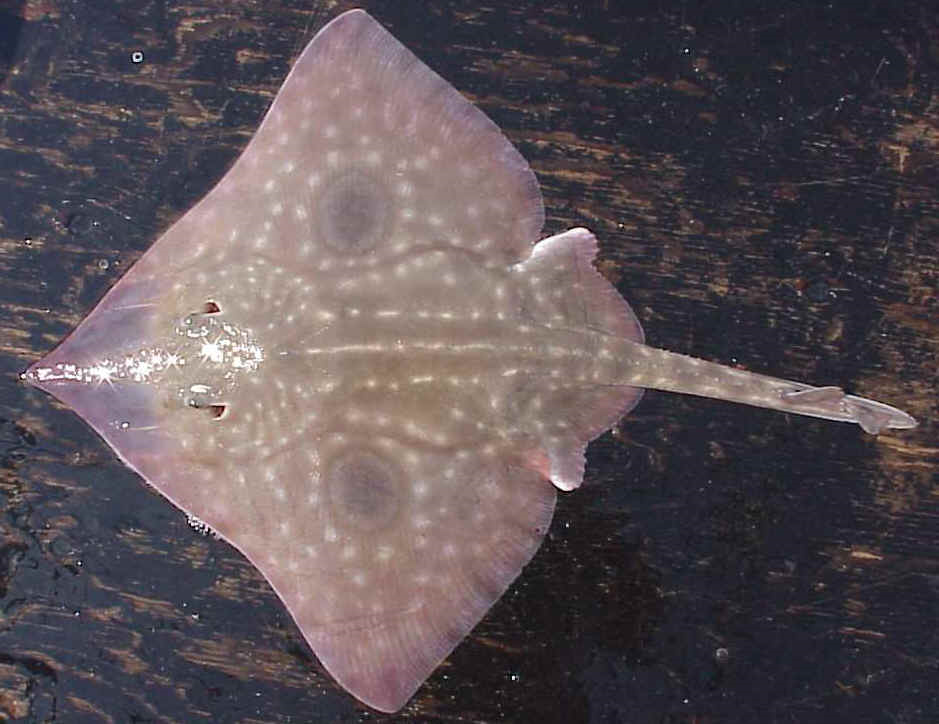
\includegraphics{cover_photo}~\\[1cm]
\pdftooltip{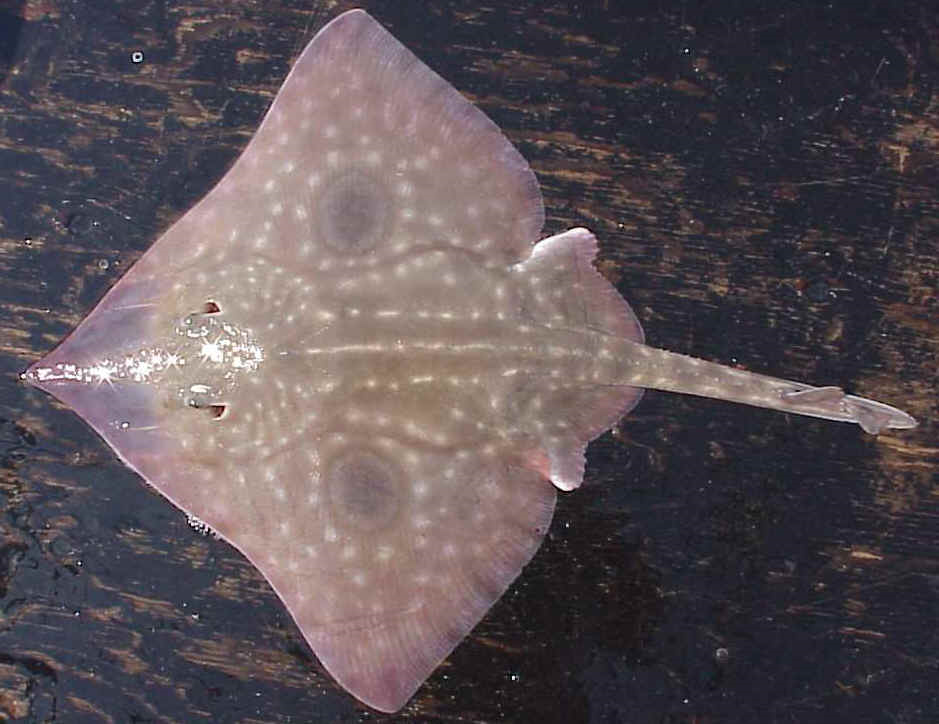
\includegraphics{cover_photo}}{This is a fish.}

\vspace{.5cm}

Ian G. Taylor\textsuperscript{1}\\
Vladlena Gertseva\textsuperscript{1}\\
Andi Stephens\textsuperscript{2}\\
Joseph Bizzarro\textsuperscript{3}\\

\vspace{.7cm}

\small

\textsuperscript{1}Northwest Fisheries Science Center, U.S. Department of Commerce, National Oceanic and Atmospheric Administration, National Marine Fisheries Service, 2725 Montlake Boulevard East, Seattle, Washington 98112\\

\vspace{.3cm}

\textsuperscript{2}Northwest Fisheries Science Center, U.S. Department of Commerce, National Oceanic and Atmospheric Administration, National Marine Fisheries Service, 2032 S.E. OSU Drive Newport, Oregon 97365

\vspace{.3cm}

\textsuperscript{3}Southwest Fisheries Science Center, U.S. Department of Commerce, National Oceanic and Atmospheric Administration, National Marine Fisheries Service, 110 Shaffer Road, Santa Cruz, California 95060\\



\vspace{.5cm}

\vfill
DRAFT SAFE\\
Disclaimer: This information is distributed solely for the purpose of pre-dissemination
peer review under applicable information quality guidelines. It has not been formally
disseminated by NOAA Fisheries. It does not represent and should not be construed to
represent any agency determination or policy. 

\vspace{.3cm}
%Bottom of the page
%{\large \today}


\newpage{\thispagestyle{empty}}

\vspace*{\fill}
\begin{flushleft}
This report may be cited as:

Taylor, I.G., Gertseva, V., Stephens, A. and Bizzarro, J. Status of Big Skate (\emph{Beringraja binoculata}) Off the U.S. West Coast, 2019. Pacific Fishery Management Council, Portland, OR. Available from http://www.pcouncil.org/groundfish/stock-assessments/
\end{flushleft}

\newpage{\thispagestyle{empty}}

% Create this table using the instructions in Acronyms.Rmd


\begin{flushleft}
\large{\textbf{Acronyms used in this Document}}
\end{flushleft}

\vspace{.5cm}

\renewcommand{\arraystretch}{1.2}

\begin{table}[ht]
% \centering
\begin{tabular}{rll}
\hline
ABC & Allowable Biological Catch \\ 
  ACL & Annual Catch Limit \\ 
  AFSC & Alaska Fisheries Science Center \\ 
  CDFW & California Department of Fish and Wildlife \\ 
  DFO & Canada's Department of Fisheries and Oceans \\ 
  DW & Disk Width \\ 
  IFQ & Individual Fishing Quota \\ 
  IPHC & International Pacific Halibut Commission \\ 
  ISW & Interspiracular Width \\ 
  NMFS & National Marine Fisheries Service \\ 
  NWFSC & Northwest Fisheries Science Center \\ 
  ODFW & Oregon Department of Fish and Wildlife \\ 
  OFL & Overfishing Limit \\ 
  OY & Optimum Yield \\ 
  PacFIN & Pacific Fisheries Information Network \\ 
  PFMC & Pacific Fishery Management Council \\ 
  SPR & Spawning Potential Ratio \\ 
  SSC & Scientific and Statistical Committee \\ 
  SWFSC & Southwest Fisheries Science Center \\ 
  TL & Total Length \\ 
  VAST & Vector Autoregressive Spatio-Temporal Package \\ 
  WCGBT & West Coast Groundfish Bottom Trawl Survey \\ 
  WCGOP & West Coast Groundfish Observer Program \\ 
  WDFW & Washington Department of Fish and Wildlife \\ 
   \hline
\end{tabular}
\end{table}

\renewcommand{\arraystretch}{1}

\maketitle

\pagenumbering{roman}
\setcounter{page}{1}
\end{center}

{
\setcounter{tocdepth}{4}
\tableofcontents
}
\setlength{\parskip}{5mm plus1mm minus1mm}
\pagebreak

\pagenumbering{arabic}

\renewcommand{\thefigure}{\alph{figure}}
\renewcommand{\thetable}{\alph{table}}

\hypertarget{executive-summary}{%
\section*{Executive Summary}\label{executive-summary}}
\addcontentsline{toc}{section}{Executive Summary}

\hypertarget{stock}{%
\subsection*{Stock}\label{stock}}
\addcontentsline{toc}{subsection}{Stock}

This assessment reports the status of the Big Skate
(\emph{Beringraja binoculata}) resource in U.S. waters off the West
Coast using data through 2018. A map showing the area of the U.S. West
Coast Exclusive Economic Zone covered by this stock assessment is
provided in Figure \ref{fig:assess_region_map}.

\begin{figure}[H]
\begin{centering}
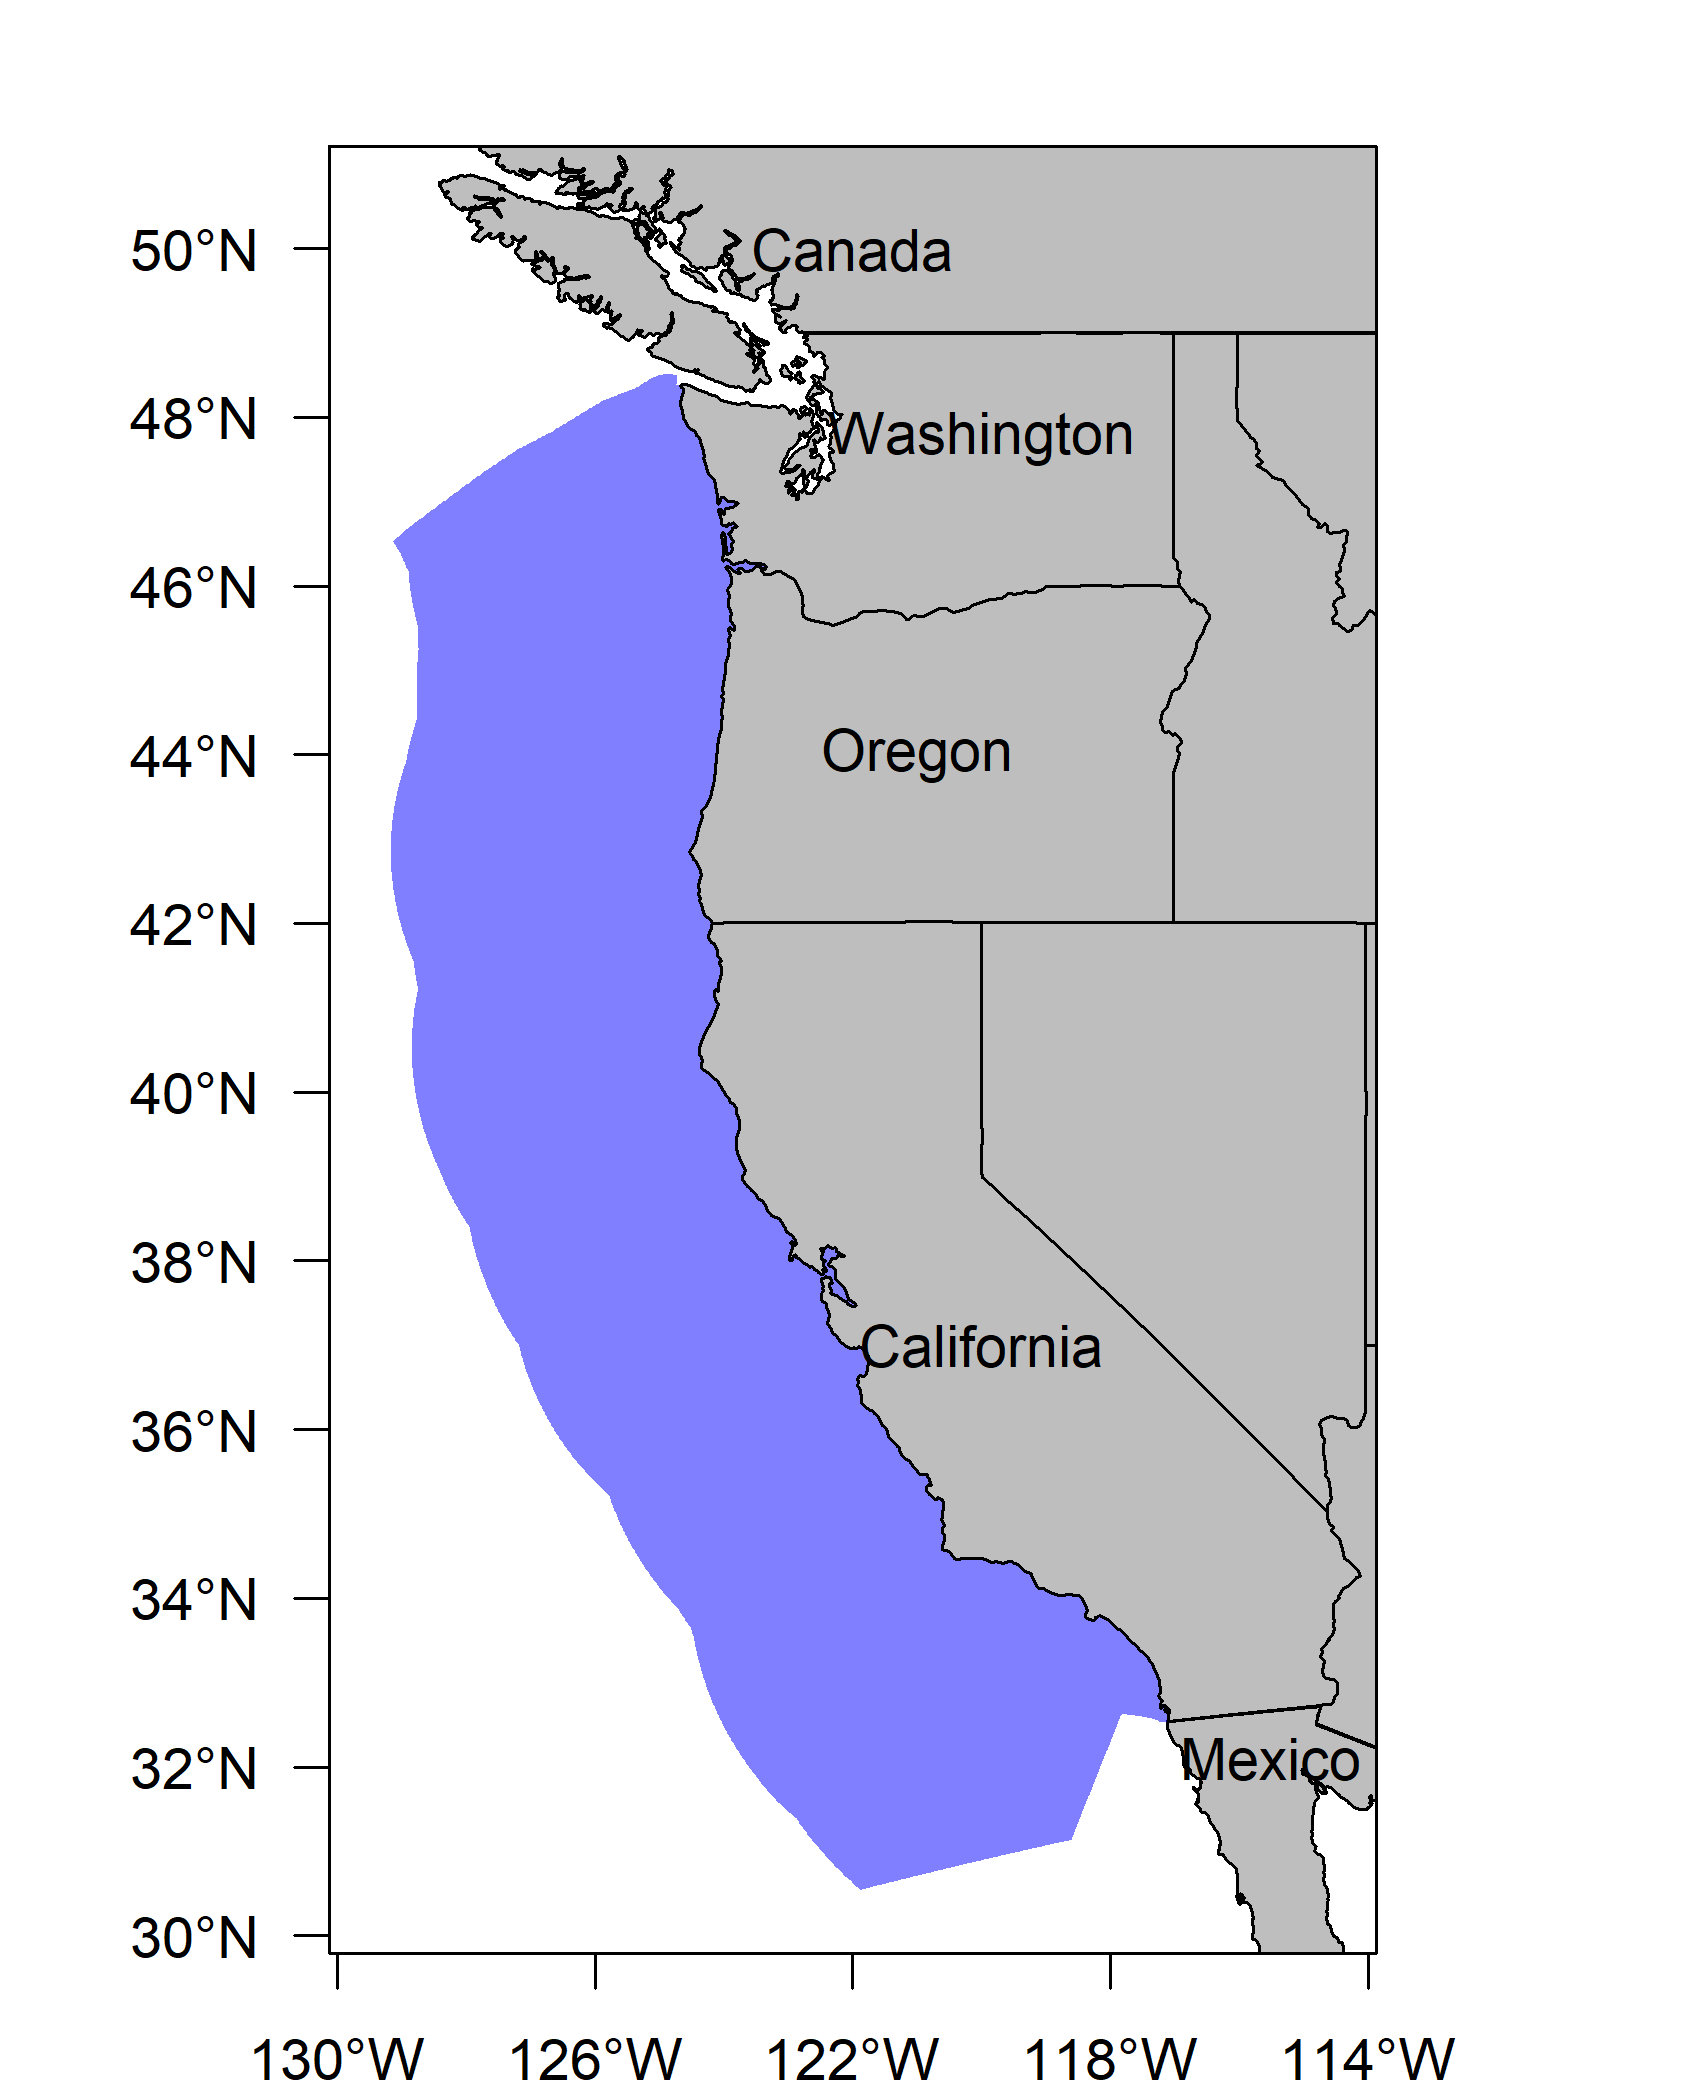
\includegraphics{Figures/assess_region_map.png}
\caption{U.S. West Coast Exclusive Economic zone covering the area in which this stock assessment is focused.}\label{fig:assess_region_map}
\end{centering}
\end{figure}

\hypertarget{catches}{%
\subsection*{Catches}\label{catches}}
\addcontentsline{toc}{subsection}{Catches}

Landings and estimated discards of Big Skate were reconstructed for this
assessment from historical records of other species and from species
composition data collected in the recent fishery. These reflect the
fishery from 1916-1994. The current fishery started in 1995. For records
from 1995-2017, Big Skate landings were estimated from
species-composition samples and the landings of ``Unspecified Skates''.
Beginning in 2017, Big Skate have been recorded in species-specific
landings.

In the current fishery (since 1995), annual total landings of Big Skate
have ranged between 135-528 mt, with landings in 2018 totaling 173 mt.

\vspace{.5cm}

\FloatBarrier

\begin{table}[ht]
\centering
\caption{Recent Big Skate landings (mt)} 
\label{tab:Exec_catch}
\begin{tabular}{>{\centering}p{1in}>{\centering}p{1in}}
  \hline
Year & Landings \\ 
  \hline
2008 & 366.00 \\ 
  2009 & 205.70 \\ 
  2010 & 196.20 \\ 
  2011 & 268.40 \\ 
  2012 & 269.60 \\ 
  2013 & 135.00 \\ 
  2014 & 372.40 \\ 
  2015 & 331.50 \\ 
  2016 & 411.50 \\ 
  2017 & 277.60 \\ 
  2018 & 172.60 \\ 
   \hline
\end{tabular}
\end{table}

\FloatBarrier

\begin{figure}
\centering
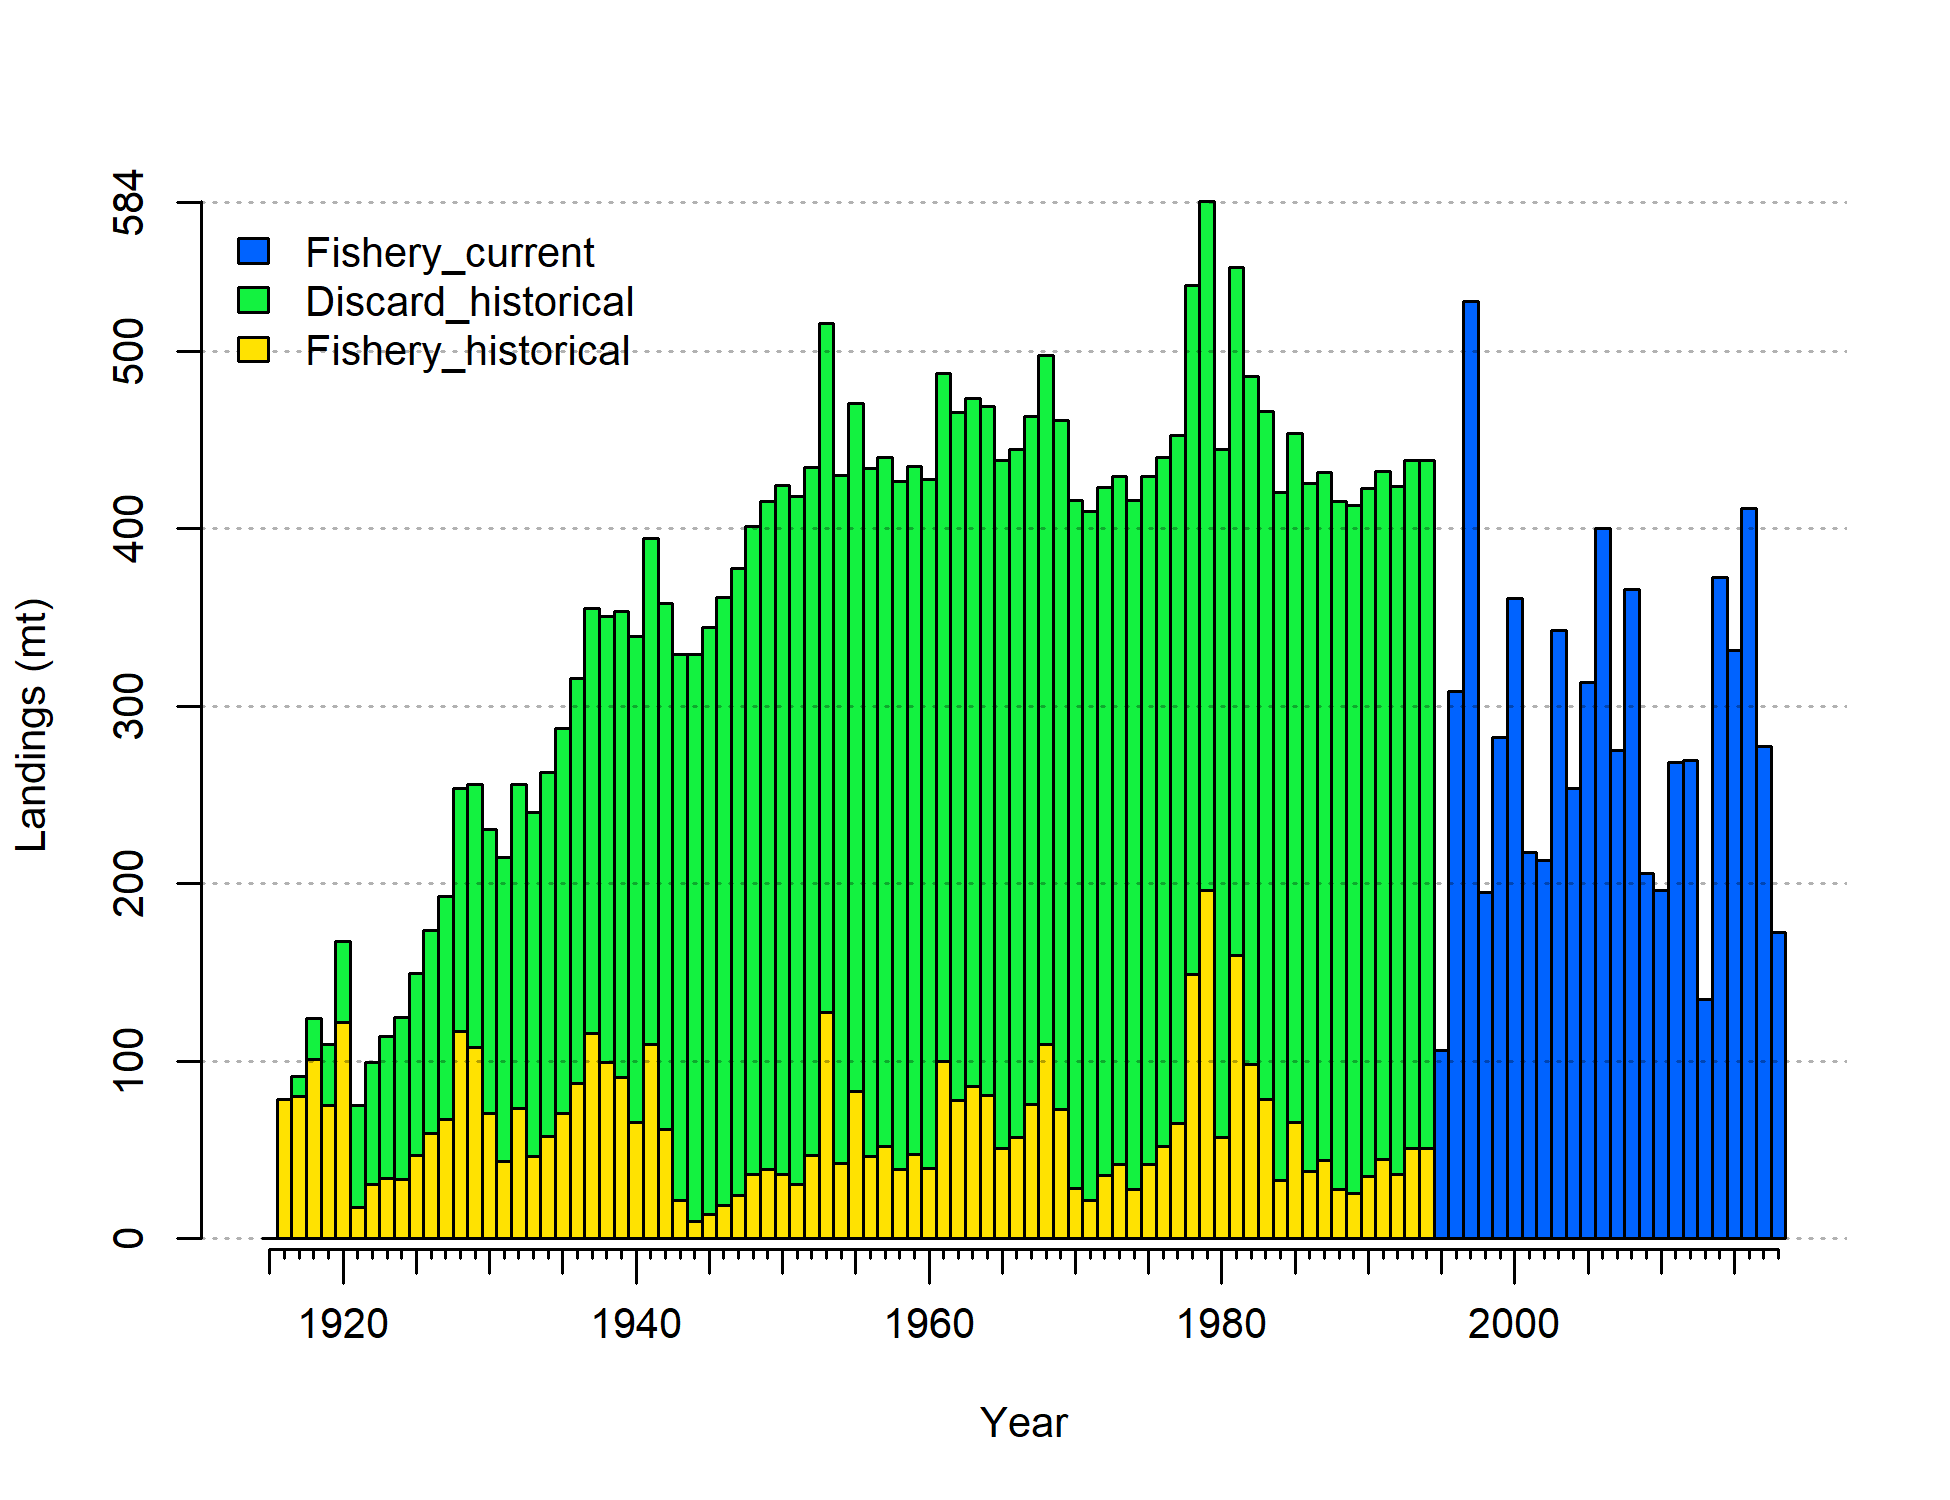
\includegraphics{r4ss/plots_mod1/catch2 landings stacked.png}
\caption{Catch history of Big Skate in the model.
\label{fig:r4ss_catches}}
\end{figure}

\FloatBarrier

\newpage

\hypertarget{data-and-assessment}{%
\subsection*{Data and Assessment}\label{data-and-assessment}}
\addcontentsline{toc}{subsection}{Data and Assessment}

This the first full assessment for Big Skate. It is currently managed
using an OFL which was based on a proxy for \(F_{MSY}\) and a 3-year
recent average of survey biomass. This assessment uses the newest
version of Stock Synthesis (3.30.13). The model begins in 1916, and
assumes the stock was at an unfished equilibrium that year.

The assessment relies on two bottom trawl survey indices of abundance,
the Triennial Survey from an index covering the period 1980--2004 was
used here and the West Coast Groundifish Bottom Trawl (WCGBT) Survey,
which began in 2003 and for which data is available through 2018. The
triennial survey shows an increasing trend over the 25 year period it
covers, which the model is not able to fit as this includes the peak
period of the fishery when the stock would have been expected to be
declining. The WCGBT Survey also shows an increasing trend, with the 5
most recent observations (2014--2018) all falling in the top 6 ever
observed (2004 was the 5th highest observation). The model estimates an
increasing trend during this period but the slope is more gradual than
the trend in the survey. The misfit to these survey indices could be due
to some combination of incorrect estimation of the catch history,
variability in recruitment which is not modeled here, or biological or
ecological changes for which data are not available.

Length composition data from the fishery is available starting in 1995
but is sparse until the past decade. Most of the ages are also from 2008
onward. This limits the ability of the model to estimate any changes
composition of the population during the majority of the history of the
fishery. Estimates of discard rates and mean body weight of discards are
available for the years 2002 onward and discard length compositions are
available starting in 2010.

The age and length data provide evidence for growth patterns and
sex-specific differences in selectivity that are unusual among
groundfish stocks that have been assessed within the U.S. West Coast and
are not found in Longnose Skate where the data show little difference
between the sexes. Growth appears to be almost linear and similar
between females and males up to about age 7 or over 100 cm at which
point male growth appears to stabilize while females continue to grow.
However, in spite of the similar growth pattern for ages prior to 7,
males are observed more frequently, with the 70--100 cm length bins
often showing 60\% males. Sex-specific differences in selectivity were
included in the model in order to better match patterns in the sex
ratios in the length composition data. The length and age data do not
cover enough years or show enough evidence of distinct cohorts to
reliably estimate deviations in recruitment around the stock-recruit
curve.

The scale of the population is not reliably informed by the data due to
the combination of surveys that show trends which can't be matched by
the structure of the model and length and age data which inform growth
and selectivity but provide relatively little information about changes
in stock structure over time. Therefore, a prior on catchability of the
WCGBT Survey (centered at 0.83) was applied in order to provide more
stable results.

Although the assessment model requires numerous simplifying assumptions,
it represents an improvement over the simplistic status-quo method of
setting management limits, which relies on average survey biomass and an
assumption about \(F_{MSY}\). The use of an age-structured model with
estimated growth, selectivity, and natural mortality likely provide a
better estimate of past dynamics and the impacts of fishing in the
future.

\hypertarget{stock-biomass}{%
\subsection*{Stock Biomass}\label{stock-biomass}}
\addcontentsline{toc}{subsection}{Stock Biomass}

The 2018 estimated spawning biomass relative to unfished equilibrium
spawning biomass is above the target of 40\% of unfished spawning
biomass at 75.0\% (95\% asymptotic interval: \(\pm\) 63.9\%-86.0\%)
(Figure \ref{fig:RelDeplete_all}). Approximate confidence intervals
based on the asymptotic variance estimates show that the uncertainty in
the estimated spawning biomass is high, although even the lower range of
the 95\% interval for \%unfished is above the 40\% reference point, and
all sensitivity analyses explore also show the stock to be at a high
level.

\vspace{.5cm}

\FloatBarrier

\begin{table}[ht]
\centering
\caption{Recent trend in beginning of the 
                                      year spawning output and %unfished
                                      (spawning biomass relative to unfished
                                      equilibrum spawning biomass)} 
\label{tab:SpawningDeplete_mod1}
\begin{tabular}{l>{\centering}p{1.3in}>{\centering}p{1.2in}>{\centering}p{1in}>{\centering}p{1.2in}}
  \hline
Year & Spawning Output (mt) & \~{} 95\% confidence interval & Estimated \%unfished & \~{} 95\% confidence interval \\ 
  \hline
2010 & 1603.690 & (726.67-2480.71) & 0.721 & (0.6-0.842) \\ 
  2011 & 1617.560 & (738.18-2496.94) & 0.727 & (0.608-0.847) \\ 
  2012 & 1625.610 & (745.16-2506.06) & 0.731 & (0.613-0.849) \\ 
  2013 & 1634.790 & (753.17-2516.41) & 0.735 & (0.618-0.852) \\ 
  2014 & 1657.340 & (772.22-2542.46) & 0.745 & (0.631-0.859) \\ 
  2015 & 1657.020 & (772.35-2541.69) & 0.745 & (0.632-0.859) \\ 
  2016 & 1659.820 & (774.79-2544.85) & 0.746 & (0.634-0.859) \\ 
  2017 & 1652.180 & (768.4-2535.96) & 0.743 & (0.63-0.856) \\ 
  2018 & 1655.400 & (770.86-2539.94) & 0.744 & (0.632-0.857) \\ 
  2019 & 1667.190 & (780.42-2553.96) & 0.750 & (0.639-0.86) \\ 
   \hline
\end{tabular}
\end{table}

\FloatBarrier

\begin{figure}
\centering
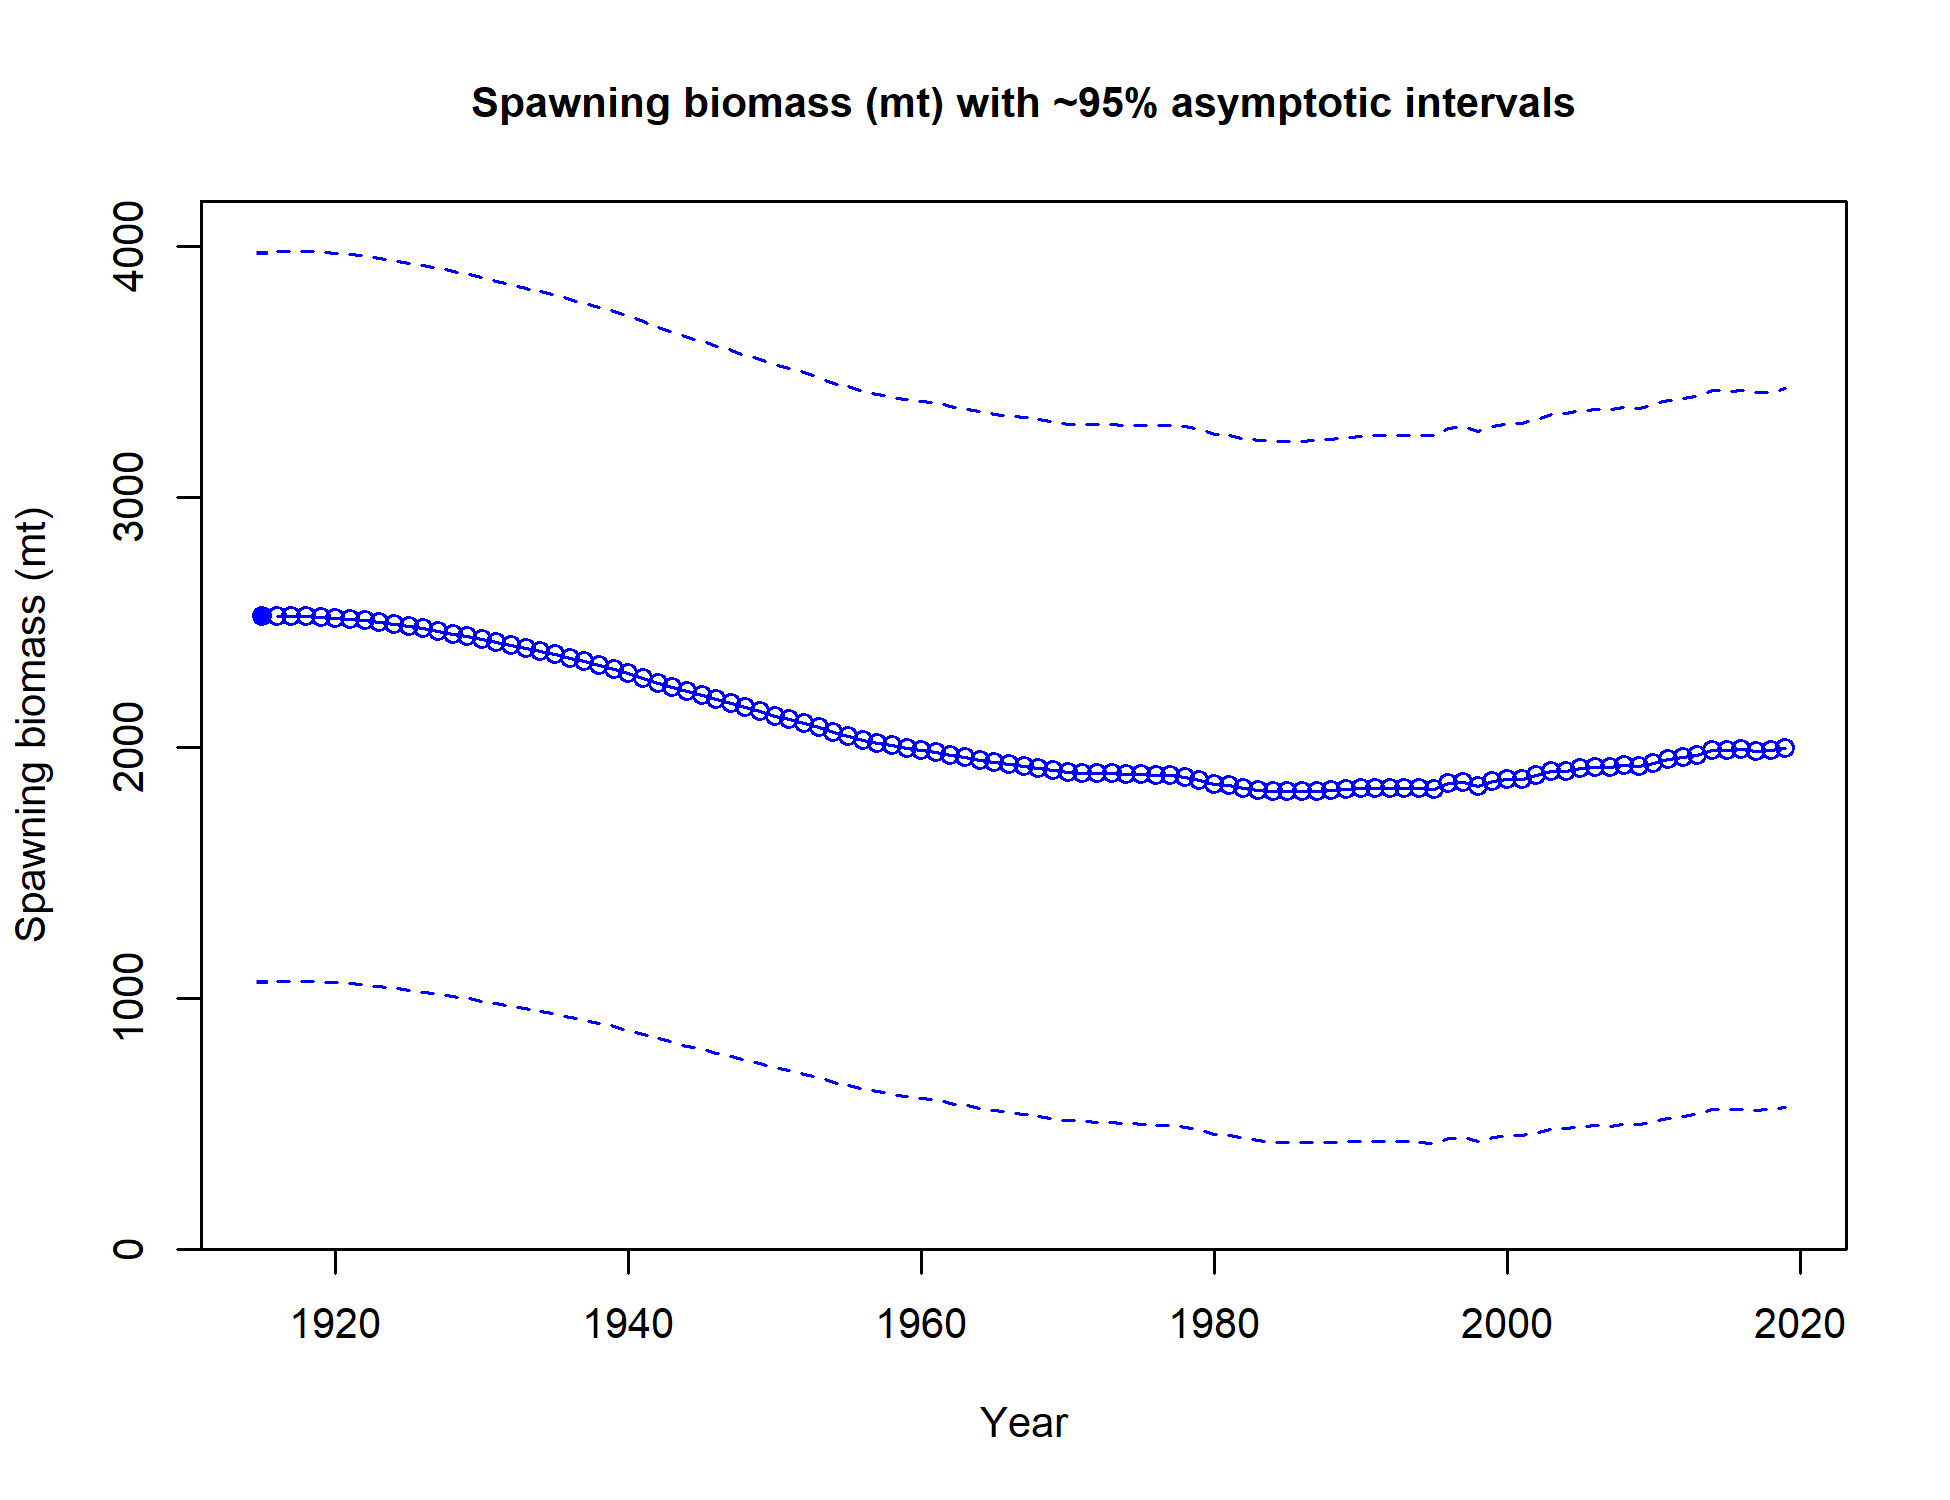
\includegraphics{r4ss/plots_mod1/ts7_Spawning_biomass_(mt)_with_95_asymptotic_intervals_intervals.png}
\caption{Time series of spawning biomass trajectory (circles and line:
median; light broken lines: 95\% credibility intervals) for the base
case assessment model. \label{fig:Spawnbio_all}}
\end{figure}

\FloatBarrier

\hypertarget{recruitment}{%
\subsection*{Recruitment}\label{recruitment}}
\addcontentsline{toc}{subsection}{Recruitment}

Recruitment was assumed to follow the Beverton-Holt stock recruit curve,
so uncertainty in estimated recruitment is due to uncertainty in
spawning biomass and the unfished equilibrium recruitment \(R_0\)
(Figure \ref{fig:Recruits_all} and Table \ref{tab:Recruit_mod1}).

\vspace{.5cm}

\begin{table}[ht]
\centering
\caption{Recent recruitment for the model.} 
\label{tab:Recruit_mod1}
\begin{tabular}{>{\centering}p{.8in}>{\centering}p{1.6in}>{\centering}p{2in}}
  \hline
Year & Estimated Recruitment (1,000s) & \~{} 95\% confidence interval \\ 
  \hline
2010 & 5393.54 & (2966.19 - 9807.3) \\ 
  2011 & 5414.62 & (2982.16 - 9831.17) \\ 
  2012 & 5426.77 & (2991.46 - 9844.65) \\ 
  2013 & 5440.55 & (3002 - 9859.94) \\ 
  2014 & 5474.01 & (3027.33 - 9898.09) \\ 
  2015 & 5473.54 & (3027.82 - 9894.77) \\ 
  2016 & 5477.66 & (3031.98 - 9896.09) \\ 
  2017 & 5466.40 & (3024.88 - 9878.58) \\ 
  2018 & 5471.15 & (3029.62 - 9880.26) \\ 
  2019 & 5488.48 & (3043.55 - 9897.46) \\ 
   \hline
\end{tabular}
\end{table}

\FloatBarrier

\begin{figure}
\centering
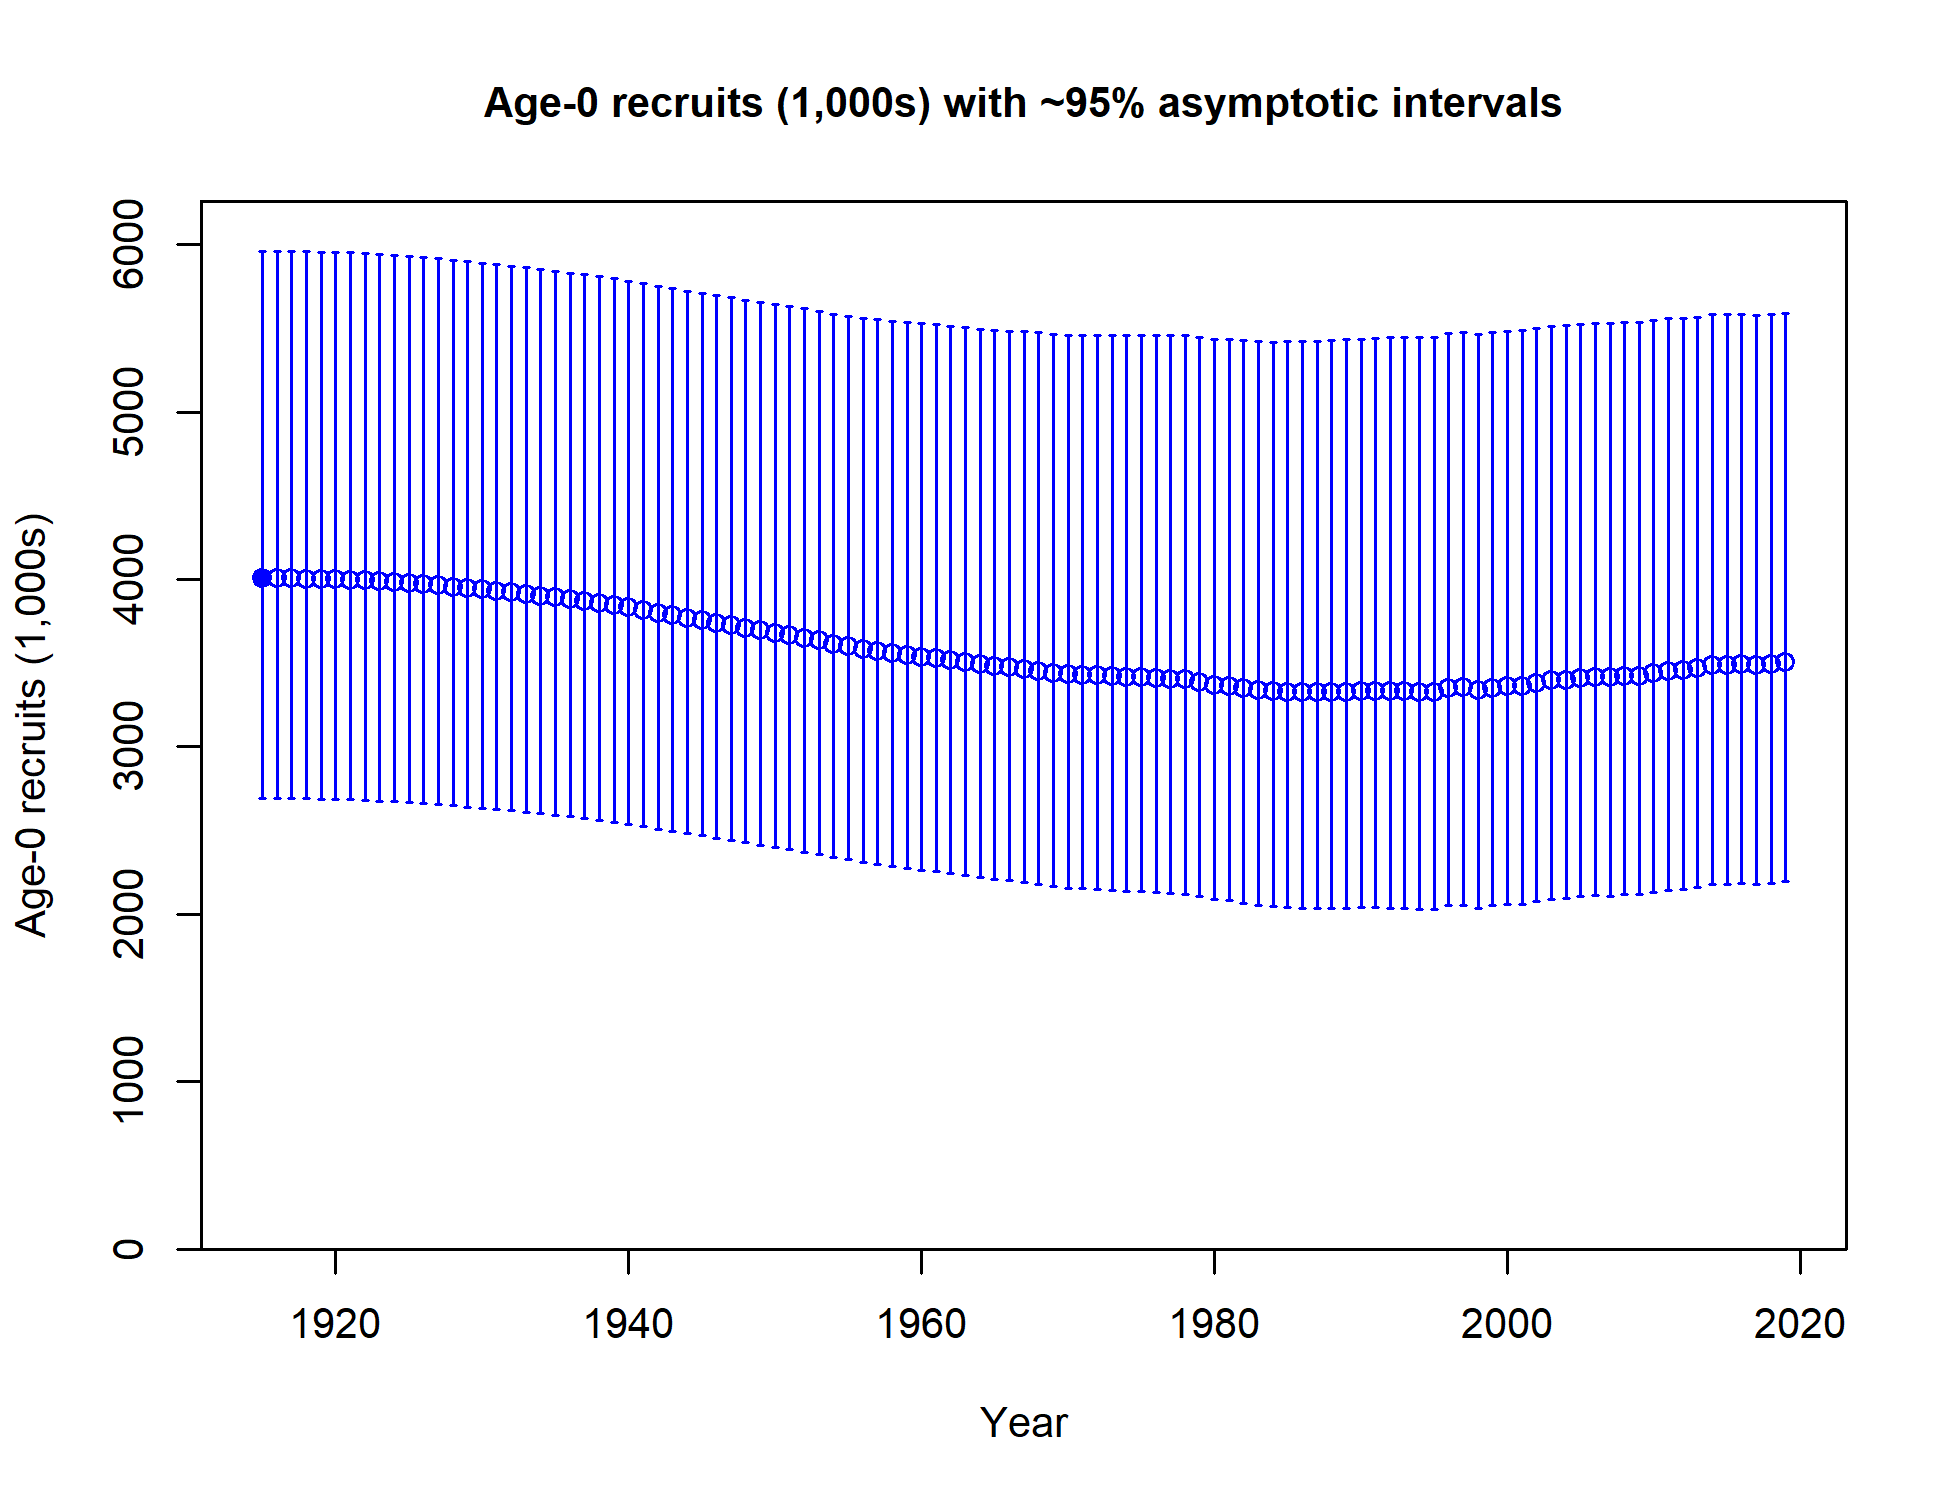
\includegraphics{r4ss/plots_mod1/ts11_Age-0_recruits_(1000s)_with_95_asymptotic_intervals.png}
\caption{Time series of estimated Big Skate recruitments for the
base-case model with 95\% confidence or credibility intervals.
\label{fig:Recruits_all}}
\end{figure}

\FloatBarrier

\hypertarget{exploitation-status}{%
\subsection*{Exploitation Status}\label{exploitation-status}}
\addcontentsline{toc}{subsection}{Exploitation Status}

Harvest rates estimated by the base model indicate catch levels have
been below the limits that would be associated with the SPR = 50\%
target (Table \ref{tab:SPR_Exploit_mod1} and Figure \ref{fig:SPR_all}).

\vspace{.5cm}

\FloatBarrier

\begin{table}[ht]
\centering
\caption{Recent trend in spawning potential 
                                        ratio and exploitation for Big Skate in the model.  Relative fishing intensity is (1-SPR) 
                                        divided by 50\% (the SPR target) and exploitation 
                                        is catch divided by age 2+ biomass.} 
\label{tab:SPR_Exploit_mod1}
\begin{tabular}{l>{\centering}p{1in}>{\centering}p{1.2in}>{\centering}p{1in}>{\centering}p{1.2in}}
  \hline
Year & Relative fishing intensity & \~{} 95\% confidence interval & Exploitation rate & \~{} 95\% confidence interval \\ 
  \hline
2009 & 0.21 & (0.12-0.3) & 0.01 & (0.01-0.02) \\ 
  2010 & 0.20 & (0.11-0.29) & 0.01 & (0.01-0.02) \\ 
  2011 & 0.26 & (0.15-0.38) & 0.01 & (0.01-0.02) \\ 
  2012 & 0.26 & (0.15-0.38) & 0.01 & (0.01-0.02) \\ 
  2013 & 0.14 & (0.08-0.2) & 0.01 & (0-0.01) \\ 
  2014 & 0.36 & (0.21-0.5) & 0.02 & (0.01-0.03) \\ 
  2015 & 0.32 & (0.19-0.45) & 0.02 & (0.01-0.03) \\ 
  2016 & 0.39 & (0.23-0.55) & 0.02 & (0.01-0.03) \\ 
  2017 & 0.28 & (0.16-0.39) & 0.02 & (0.01-0.02) \\ 
  2018 & 0.18 & (0.1-0.25) & 0.01 & (0.01-0.01) \\ 
   \hline
\end{tabular}
\end{table}

\FloatBarrier

\begin{figure}
\centering
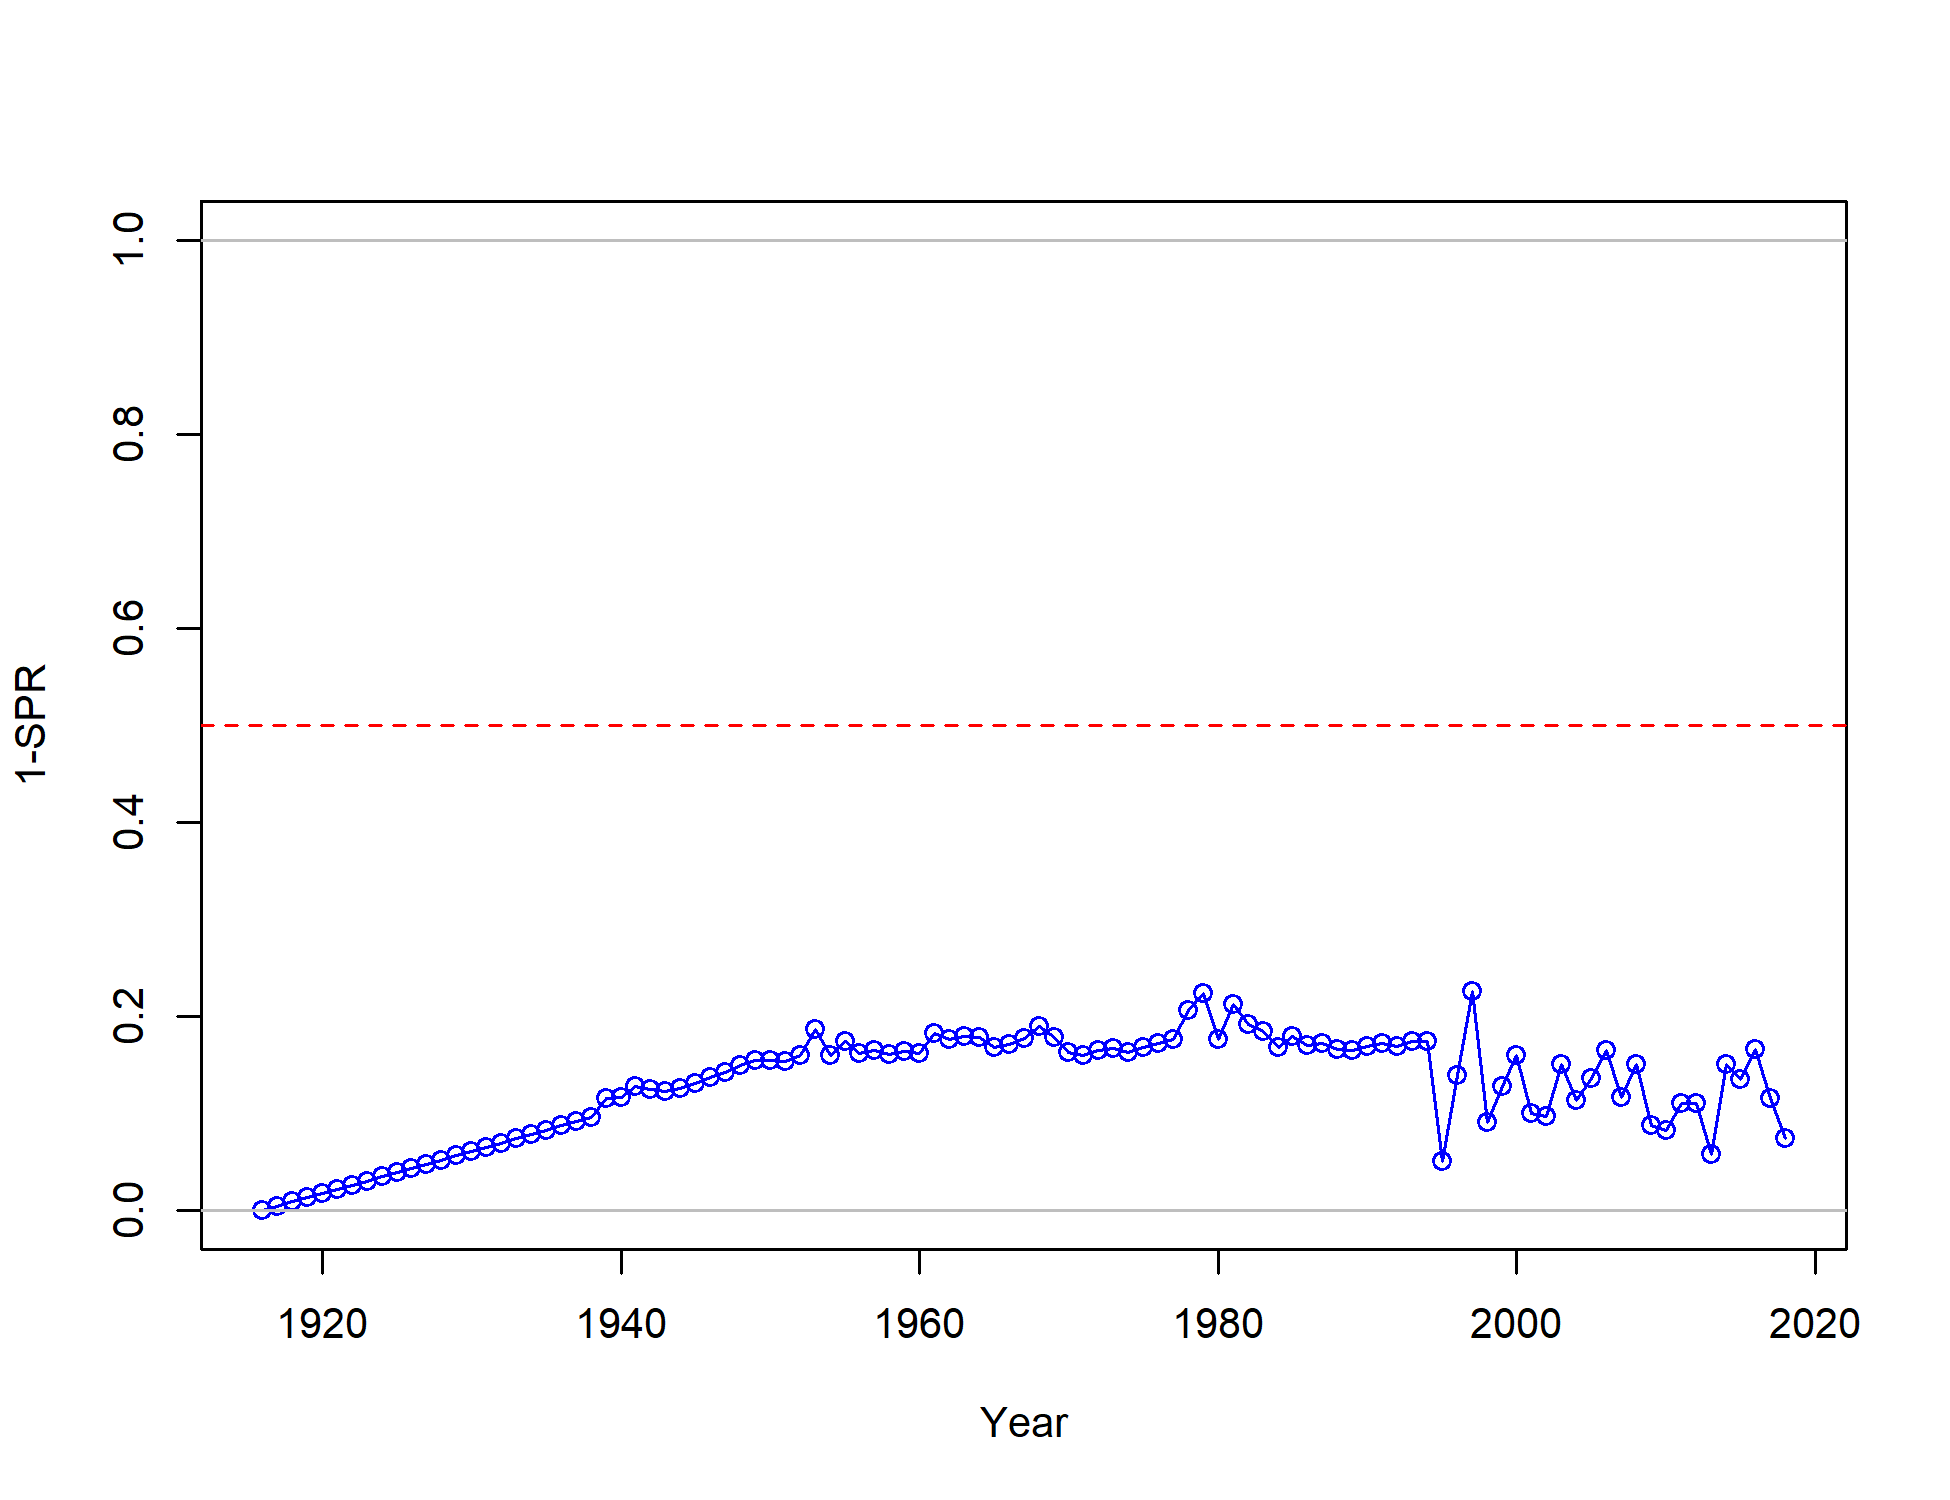
\includegraphics{r4ss/plots_mod1/SPR2_minusSPRseries.png}
\caption{Estimated spawning potential ratio (SPR) for the base-case
model. One minus SPR is plotted so that higher exploitation rates occur
on the upper portion of the y-axis. The management target is plotted as
a red horizontal line and values above this reflect harvests in excess
of the overfishing proxy based on the SPR\textsubscript{50\%} harvest
rate. The last year in the time series is 2018. \label{fig:SPR_all}}
\end{figure}

\FloatBarrier

\hypertarget{reference-points}\)), and well above the minimum stock size
threshold (\(SB_{25\%}\)). The estimated \%unfished level for the base
model in 2019 is 75.0\% (95\% asymptotic interval: \(\pm\)
63.9\%-86.0\%, corresponding to an unfished spawning biomass of 1667.19
mt (95\% asymptotic interval: 780.42-2553.96 mt) of spawning biomass in
the base model (Table \ref{tab:Ref_pts_mod1}). Unfished age 2+ biomass
was estimated to be 2,523 mt in the base case model. The target spawning
biomass (\(SB_{40\%}\)) is 890 mt, which corresponds with an equilibrium
yield of 602 mt. Equilibrium yield at the proxy \(F_{MSY}\) harvest rate
corresponding to \(SPR_{50\%}\) is 507 mt (Figure \ref{fig:Yield_all}).

\vspace{.5cm}

\FloatBarrier

\begin{table}[ht]
\centering
\caption{Summary of reference 
                                      points and management quantities for the 
                                      base case model.} 
\label{tab:Ref_pts_mod1}
\begin{tabular}{>{\raggedright}p{4.1in}>{\raggedleft}p{.62in}>{\raggedleft}p{.62in}>{\raggedleft}p{.62in}}
  \hline
\textbf{Quantity} & \textbf{Estimate} & \textbf{Low 2.5\%  limit} & \textbf{High 2.5\%  limit} \\ 
  \hline
Unfished spawning output (mt) & 2,224 & 1,246 & 3,202 \\ 
  Unfished age 2+ biomass (mt) & 2,523 & 1,705 & 3,341 \\ 
  Unfished recruitment ($R_{0}$) & 6,176 & 2,760 & 9,592 \\ 
  Spawning output(2018 mt) & 1,655 & 771 & 2,540 \\ 
  Depletion (2018) & 0.744 & 0.632 & 0.857 \\ 
  \textbf{$\text{Reference points based on } \mathbf{SB_{40\%}}$} &  &  &  \\ 
  Proxy spawning output ($B_{40\%}$) & 890 & 498 & 1,281 \\ 
  SPR resulting in $B_{40\%}$ ($SPR_{B40\%}$) & 0.625 & 0.625 & 0.625 \\ 
  Exploitation rate resulting in $B_{40\%}$ & 0.048 & 0.042 & 0.055 \\ 
  Yield with $SPR_{B40\%}$ at $B_{40\%}$ (mt) & 602 & 395 & 810 \\ 
  \textbf{\textit{Reference points based on SPR proxy for MSY}} &  &  &  \\ 
  Spawning output & 445 & 249 & 640 \\ 
  $SPR_{proxy}$ & 0.5 &  &  \\ 
  Exploitation rate corresponding to $SPR_{proxy}$ & 0.071 & 0.061 & 0.08 \\ 
  Yield with $SPR_{proxy}$ at $SB_{SPR}$ (mt) & 507 & 333 & 681 \\ 
  \textbf{\textit{Reference points based on estimated MSY values}} &  &  &  \\ 
  Spawning output at $MSY$ ($SB_{MSY}$) & 833 & 458 & 1,207 \\ 
  $SPR_{MSY}$ & 0.609 & 0.604 & 0.614 \\ 
  Exploitation rate at $MSY$ & 0.051 & 0.045 & 0.057 \\ 
  Dead Catch $MSY$ (mt) & 604 & 396 & 812 \\ 
  Retained Catch $MSY$ (mt) & 559 & 367 & 750 \\ 
   \hline
\end{tabular}
\end{table}

\FloatBarrier

\newpage

\hypertarget{ecosystem-considerations}{%
\subsection*{Ecosystem Considerations}\label{ecosystem-considerations}}
\addcontentsline{toc}{subsection}{Ecosystem Considerations}

In this assessment, neither environmental nor ecosystem considerations
were explicitly included in the analysis. This is primarily due to a
lack of relevant data or results of analyses that could contribute
ecosystem-related quantitative information for the assessment.

\hypertarget{management-performance}{%
\subsection*{Management Performance}\label{management-performance}}
\addcontentsline{toc}{subsection}{Management Performance}

\begin{table}[ht]
\centering
\caption{Recent trend in total catch (mt) relative to the 
                              management guidelines. Big skate was
                              managed in the Other Species complex in 2013 and 2014,
                              designated an Ecosystem Component species in 2015 and
                              2016, and managed with stock-specific harvest
                              specifications since 2017.} 
\label{tab:mnmgt_perform}
\scalebox{0.9}{
\begin{tabular}{l>{\centering}p{1.2in}>{\centering}p{1in}>{\centering}p{1in}>{\centering}p{1in}}
  \hline
Year & OFL (mt; ABC prior to 2011) & ABC (mt) & ACL (mt; OY prior to 2011) & Estimated total catch (mt) \\ 
  \hline
\textbf{2009} &  &  &  & 205.70 \\ 
  \textbf{2010} &  &  &  & 196.20 \\ 
  \textbf{2011} &  &  &  & 268.40 \\ 
  \textbf{2012} &  &  &  & 269.60 \\ 
  \textbf{2013} & 458.00 & 317.90 & 317.90 & 135.00 \\ 
  \textbf{2014} & 458.00 & 317.90 & 317.90 & 372.40 \\ 
  \textbf{2015} &  &  &  & 331.50 \\ 
  \textbf{2016} &  &  &  & 411.50 \\ 
  \textbf{2017} & 541.00 & 494.00 & 494.00 & 277.60 \\ 
  \textbf{2018} & 541.00 & 494.00 & 494.00 & 172.60 \\ 
  \textbf{2019} & 541.00 & 494.00 & 494.00 &  \\ 
  \textbf{2020} & 541.00 & 494.00 & 494.00 &  \\ 
   \hline
\end{tabular}
}
\end{table}

\FloatBarrier

\hypertarget{unresolved-problems-and-major-uncertainties}{%
\subsection*{Unresolved Problems and Major
Uncertainties}\label{unresolved-problems-and-major-uncertainties}}
\addcontentsline{toc}{subsection}{Unresolved Problems and Major
Uncertainties}

The data provide little information about the scale of the population,
necessitating the use of a prior on catchability to maintain stable
model results. The prior was developed for the 2007 Longnose Skate stock
assessment and has not been revised to account for any differences
between the two species.

There is little evidence that the population is overfished or
experiencing overfishing, but forecasts of overfishing limits vary
considerably among the sensitivity analyses explored (though all remain
well above the recent average catch).

The fit to the length data was significantly improved by estimating a
difference between female and male selectivity, with females having a
lower maximum selectivity than males, but the behavioral processes that
might contribute to this difference are not understood.

\FloatBarrier

\hypertarget{decision-table}{%
\subsection*{Decision Table}\label{decision-table}}
\addcontentsline{toc}{subsection}{Decision Table}

\textbf{\(\color{red}{\text{Template in Table h and associated discussion to be filled in during the STAR panel}}\)}

\FloatBarrier

\hypertarget{projected-landings-ofls-and-time-varying-acls}{%
\subsection*{Projected Landings, OFLs and Time-varying
ACLs}\label{projected-landings-ofls-and-time-varying-acls}}
\addcontentsline{toc}{subsection}{Projected Landings, OFLs and
Time-varying ACLs}

Potential OFLs projected by the model are shown in Table
\ref{tab:OFL_projection}. These values are based on an SPR target of
50\%, a P* of 0.45, and a time-varying Category 2 Sigma which creates
the buffer shown in the right-hand column.

\begin{table}[ht]
\centering
\caption{Projections of landings, total mortality, OFL, and ACL values.} 
\label{tab:OFL_projection}
\begin{tabular}{l>{\centering}p{0.8in}>{\centering}p{1.2in}>{\centering}p{0.8in}>{\centering}p{0.8in}>{\centering}p{0.8in}}
  \hline
Year & Landings (mt) & Estimated total mortality (mt) & OFL (mt) & ACL (mt) & Buffer \\ 
  \hline
2019 & 313.16 & 336.35 & 541.00 & 494.00 & 1.00 \\ 
  2020 & 313.16 & 336.32 & 541.00 & 494.00 & 1.00 \\ 
  2021 & 1042.23 & 1119.74 & 1275.51 & 1119.75 & 0.87 \\ 
  2022 & 987.51 & 1062.58 & 1222.62 & 1062.58 & 0.86 \\ 
  2023 & 942.80 & 1015.91 & 1179.51 & 1015.91 & 0.86 \\ 
  2024 & 906.41 & 977.59 & 1145.41 & 977.59 & 0.85 \\ 
  2025 & 876.49 & 945.64 & 1118.21 & 945.64 & 0.84 \\ 
  2026 & 850.59 & 917.76 & 1095.36 & 917.76 & 0.83 \\ 
  2027 & 828.05 & 893.39 & 1075.04 & 893.39 & 0.83 \\ 
  2028 & 805.87 & 869.37 & 1056.06 & 869.37 & 0.82 \\ 
  2029 & 784.60 & 846.33 & 1037.94 & 846.33 & 0.81 \\ 
  2030 & 764.95 & 825.07 & 1020.44 & 825.07 & 0.80 \\ 
   \hline
\end{tabular}
\end{table}
\begin{table}[ht]
\centering
\caption{Summary of 10-year 
                                             projections beginning in 2020 
                                             for alternate states of nature based on 
                                             an axis of uncertainty for the model.  Columns range over low, mid, and high
                                             states of nature, and rows range over different 
                                             assumptions of catch levels. An entry of "--" 
                                             indicates that the stock is driven to very low 
                                             abundance under the particular scenario.} 
\label{tab:Decision_table_mod1}
\scalebox{0.85}{
\begin{tabular}{l|cc|>{\centering}p{.7in}c|>{\centering}p{.7in}c|>{\centering}p{.7in}c}
   \multicolumn{3}{c}{}  &  \multicolumn{2}{c}{} 
                               & \multicolumn{2}{c}{\textbf{States of nature}} 
                               & \multicolumn{2}{c}{} \\
  \multicolumn{3}{c}{}  &  \multicolumn{2}{c}{Low State} 
                               & \multicolumn{2}{c}{Base State} 
                               &  \multicolumn{2}{c}{High State} \\
 \hline
 & Year & Catch & Spawning Output & Depletion & Spawning Output & Depletion & Spawning Output & Depletion \\ 
  \hline
 & 2019 & - & - & - & - & - & - & - \\ 
   & 2020 & - & - & - & - & - & - & - \\ 
   & 2021 & - & - & - & - & - & - & - \\ 
  Default harvest,  & 2022 & - & - & - & - & - & - & - \\ 
  for Low State & 2023 & - & - & - & - & - & - & - \\ 
   & 2024 & - & - & - & - & - & - & - \\ 
   & 2025 & - & - & - & - & - & - & - \\ 
   & 2026 & - & - & - & - & - & - & - \\ 
   & 2027 & - & - & - & - & - & - & - \\ 
   & 2028 & - & - & - & - & - & - & - \\ 
   \hline
 & 2019 & - & - & - & - & - & - & - \\ 
   & 2020 & - & - & - & - & - & - & - \\ 
   & 2021 & - & - & - & - & - & - & - \\ 
  Default harvest,  & 2022 & - & - & - & - & - & - & - \\ 
  for Base State & 2023 & - & - & - & - & - & - & - \\ 
   & 2024 & - & - & - & - & - & - & - \\ 
   & 2025 & - & - & - & - & - & - & - \\ 
   & 2026 & - & - & - & - & - & - & - \\ 
   & 2027 & - & - & - & - & - & - & - \\ 
   & 2028 & - & - & - & - & - & - & - \\ 
   \hline
 & 2019 & - & - & - & - & - & - & - \\ 
   & 2020 & - & - & - & - & - & - & - \\ 
   & 2021 & - & - & - & - & - & - & - \\ 
  Default harvest,  & 2022 & - & - & - & - & - & - & - \\ 
  for High State & 2023 & - & - & - & - & - & - & - \\ 
   & 2024 & - & - & - & - & - & - & - \\ 
   & 2025 & - & - & - & - & - & - & - \\ 
   & 2026 & - & - & - & - & - & - & - \\ 
   & 2027 & - & - & - & - & - & - & - \\ 
   & 2028 & - & - & - & - & - & - & - \\ 
   \hline
 & 2019 & - & - & - & - & - & - & - \\ 
   & 2020 & - & - & - & - & - & - & - \\ 
   & 2021 & - & - & - & - & - & - & - \\ 
  Average & 2022 & - & - & - & - & - & - & - \\ 
  Catch & 2023 & - & - & - & - & - & - & - \\ 
   & 2024 & - & - & - & - & - & - & - \\ 
   & 2025 & - & - & - & - & - & - & - \\ 
   & 2026 & - & - & - & - & - & - & - \\ 
   & 2027 & - & - & - & - & - & - & - \\ 
   & 2028 & - & - & - & - & - & - & - \\ 
   \hline
\end{tabular}
}
\end{table}
\FloatBarrier

\newgeometry{hmargin=1in,vmargin=1in}

\begin{landscape}

\renewcommand{\arraystretch}{1.2}
\begin{table}[ht]
\centering
\caption{Base case results summary.} 
\label{tab:base_summary}
\scalebox{0.6}{
\begin{tabular}{r>{\centering}p{1.1in}>{\centering}p{1.1in}>{\centering}p{1.1in}>{\centering}p{1.1in}>{\centering}p{1.1in}>{\centering}p{1.1in}>{\centering}p{1.1in}>{\centering}p{1.1in}>{\centering}p{1.1in}>{\centering}p{1.1in}}
  \hline
Quantity & 2010 & 2011 & 2012 & 2013 & 2014 & 2015 & 2016 & 2017 & 2018 & 2019 \\ 
  \hline
Landings (mt) &  313.160 &  313.160 & 1042.228 &  987.509 &  942.796 &  906.409 &  876.485 &  850.594 &  828.055 &  805.865 \\ 
  Total Est. Catch (mt) &  336.345 &  336.325 & 1119.745 & 1062.581 & 1015.907 &  977.592 &  945.644 &  917.761 &  893.393 &  869.365 \\ 
  OFL (mt) &  541.00 &  541.00 & 1275.51 & 1222.62 & 1179.51 & 1145.41 & 1118.21 & 1095.36 & 1075.04 & 1056.06 \\ 
  ACL (mt) &  494.000 &  494.000 & 1119.750 & 1062.580 & 1015.910 &  977.592 &  945.643 &  917.762 &  893.393 &  869.365 \\ 
   \hline
(1-$SPR$)(1-$SPR_{50\%}$) & 0.20 & 0.26 & 0.26 & 0.14 & 0.36 & 0.32 & 0.39 & 0.28 & 0.18 &  \\ 
   \hline
Exploitation rate & 0.01 & 0.01 & 0.01 & 0.01 & 0.02 & 0.02 & 0.02 & 0.02 & 0.01 &  \\ 
  Age 2+ biomass (mt) & 18810.9 & 18968.2 & 19113.5 & 19171.0 & 19221.9 & 19394.4 & 19315.6 & 19300.1 & 19211.4 & 19275.8 \\ 
   \hline
Spawning Output & 1603.7 & 1617.6 & 1625.6 & 1634.8 & 1657.3 & 1657.0 & 1659.8 & 1652.2 & 1655.4 & 1667.2 \\ 
  ~95\% CI & (726.67-2480.71) & (738.18-2496.94) & (745.16-2506.06) & (753.17-2516.41) & (772.22-2542.46) & (772.35-2541.69) & (774.79-2544.85) & (768.4-2535.96) & (770.86-2539.94) & (780.42-2553.96) \\ 
   \hline
Depletion & 0.7 & 0.7 & 0.7 & 0.7 & 0.7 & 0.7 & 0.7 & 0.7 & 0.7 & 0.7 \\ 
  ~95\% CI & (0.6-0.842) & (0.608-0.847) & (0.613-0.849) & (0.618-0.852) & (0.631-0.859) & (0.632-0.859) & (0.634-0.859) & (0.63-0.856) & (0.632-0.857) & (0.639-0.86) \\ 
   \hline
Recruits & 5393.54 & 5414.62 & 5426.77 & 5440.55 & 5474.01 & 5473.54 & 5477.66 & 5466.40 & 5471.15 & 5488.48 \\ 
  ~95\% CI & (2966.19 - 9807.3) & (2982.16 - 9831.17) & (2991.46 - 9844.65) & (3002 - 9859.94) & (3027.33 - 9898.09) & (3027.82 - 9894.77) & (3031.98 - 9896.09) & (3024.88 - 9878.58) & (3029.62 - 9880.26) & (3043.55 - 9897.46) \\ 
   \hline
\end{tabular}
}
\end{table}
\renewcommand{\arraystretch}{1}
\end{landscape}
\restoregeometry

\begin{figure}
\centering
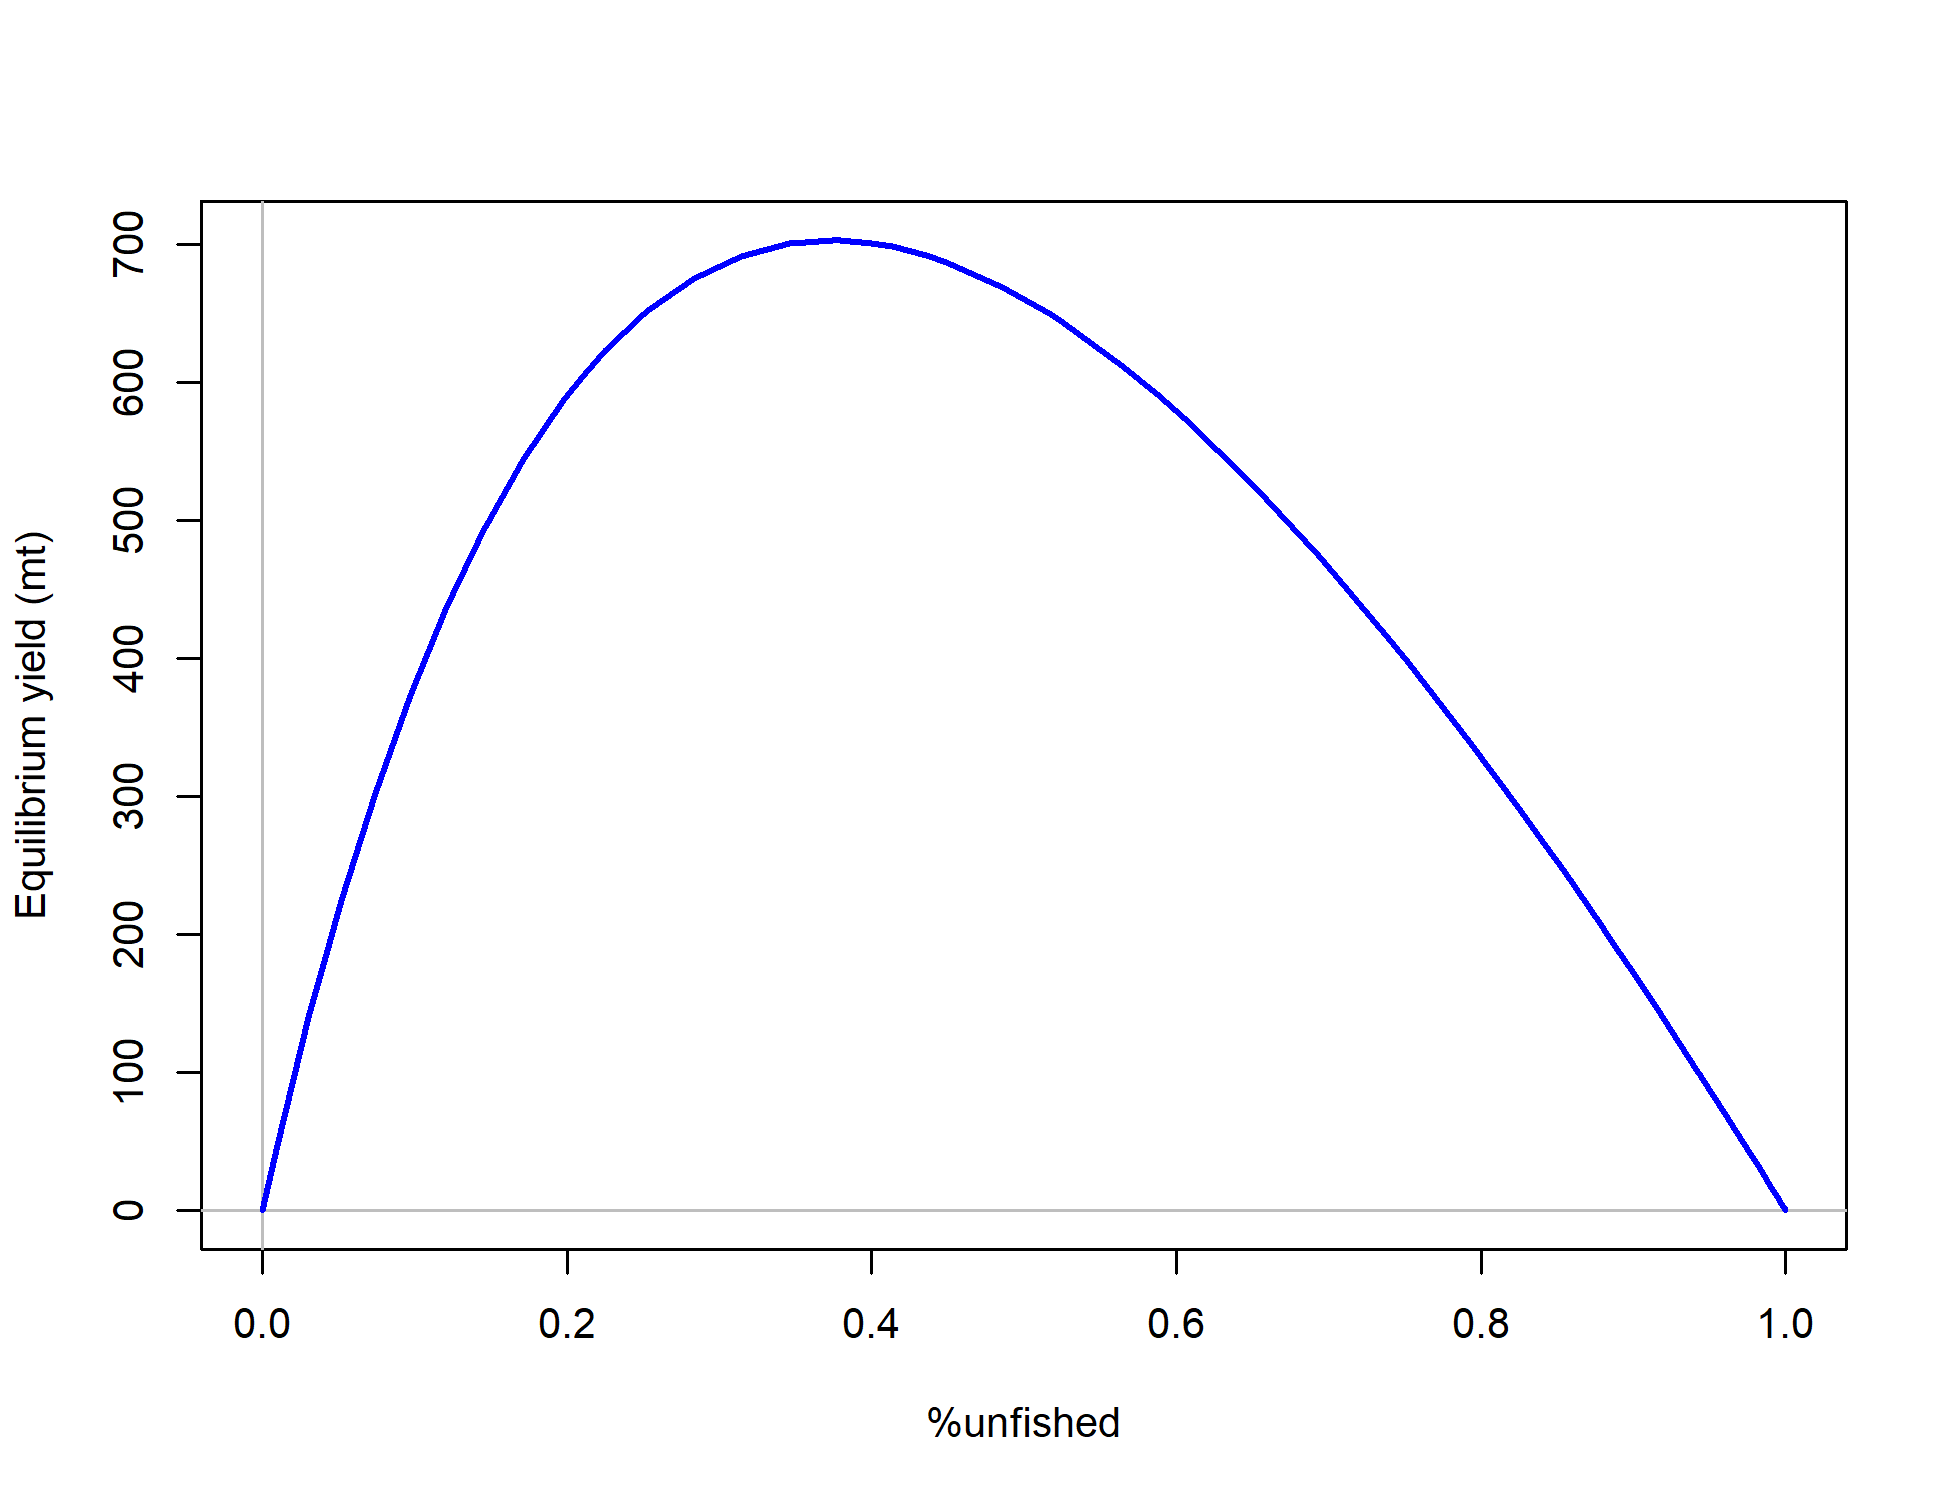
\includegraphics{r4ss/plots_mod1/yield1_yield_curve.png}
\caption{Equilibrium yield curve for the base case model. Values are
based on the 2018 fishery selectivity and with steepness fixed at 0.718.
\label{fig:Yield_all}}
\end{figure}

\FloatBarrier

\newpage

\hypertarget{research-and-data-needs}{%
\subsection*{Research and Data Needs}\label{research-and-data-needs}}
\addcontentsline{toc}{subsection}{Research and Data Needs}

We recommend the following research be conducted before the next
assessment:

\begin{enumerate}

\item \textbf{Data!}: 

\item \textbf{xxxx}:

\item \textbf{xxxx}:

\item \textbf{xxxx}:

\item \textbf{xxxx}:

\end{enumerate}

\textbf{\(\color{red}{\text{To be continued}}\)}

\FloatBarrier

\newpage
\renewcommand{\thefigure}{\arabic{figure}}
\renewcommand{\thetable}{\arabic{table}}
\setcounter{figure}{0}
\setcounter{table}{0}

\newpage
\renewcommand{\thefigure}{\arabic{figure}}
\renewcommand{\thetable}{\arabic{table}}
\setcounter{figure}{0}
\setcounter{table}{0}

\hypertarget{introduction}{%
\section{Introduction}\label{introduction}}

Skates are the largest and most widely distributed group of batoid fish
with approximately 245 species ascribed to two families (Ebert and
Compagno (\protect\hyperlink{ref-Ebert2007}{2007}), McEachran and Miyake
(\protect\hyperlink{ref-McEachran1990}{1990})). Skates are benthic fish
that are found in all coastal waters but are most common in cold
temperatures and polar waters (Ebert and Compagno
\protect\hyperlink{ref-Ebert2007}{2007}).

There are eleven species of skates in three genera (Amblyraja,
Bathyraja, and Raja) present in the Northeast Pacific Ocean off
California, Oregon and Washington (Ebert 2003). Of that number, just
three species (Longnose Skate, \emph{Raja rhina}; Big Skate, \emph{Raja
binoculata}; and Sandpaper Skate, \emph{Bathyraja interrupta}) make up
over 95 percent of West Coast Groundfish Bottom Trawl Survey (WCGBTS)
catches in terms of biomass and numbers, with the Longnose Skate leading
in both categories (with 62 percent of biomass and 56 percent of
numbers).

Big Skate (\emph{Raja binoculata}) is the largest of the skate species
in North America with a documented maximum length of 244 cm total length
and a maximum weight of 91 kg (Eschmeyer and Herald
\protect\hyperlink{ref-Eschmeyer1983}{1983}). The species name
``binoculata'' (two-eyed) refers to the prominent ocellus at the base of
each pectoral fin. Big Skates are usually seen buried in sediment with
only their eyes showing.

\hypertarget{biology}{%
\subsection{Biology}\label{biology}}

Big Skate is oviparious, and is one of two skate species that have
multiple embryos per egg case (Ebert et al.
\protect\hyperlink{ref-Ebert2008}{2008}). From 1--8 embryos can be
contained in a single, large egg capsule, but most have 3--4 (DeLacy and
Chapman \protect\hyperlink{ref-DeLacy1935}{1935}, Hitz
\protect\hyperlink{ref-Hitz1964}{1964}, Ford
\protect\hyperlink{ref-Ford1971}{1971}). Eggs are deposited year-round
on sand or mud substrates at depths of \textasciitilde{}50--150 m (Hitz
\protect\hyperlink{ref-Hitz1964}{1964}, Ebert and Compagno
\protect\hyperlink{ref-Ebert2007}{2007}). Embryos hatch from eggs after
6--20 months, with shorter developmental periods associated with warmer
temperatures (Hoff, GR \protect\hyperlink{ref-Hoff2009}{2009}). In
captivity, Big Skate females may produce \textgreater{} 350 eggs/year
(average of 2 embryos/egg case; Chiquillo, Kelcie L and Ebert, David A
and Slager, Christina J and Crow, Karen D
(\protect\hyperlink{ref-Chiquillo2014}{2014})) from long-term sperm
storage . Size at birth is 18--23 cm TL (Ebert
\protect\hyperlink{ref-Ebert2003}{2003}). Maximum size is 244 cm TL
{[}Eschmeyer and Herald (\protect\hyperlink{ref-Eschmeyer1983}{1983}),
with females growing to larger sizes.

Size at maturity has been variably estimated for Big Skate populations
off California, British Columbia, and Alaska. Off central California,
Zeiner and Wolf (\protect\hyperlink{ref-ZeinerWolf1993}{1993}) reported
sizes at first maturity of \textasciitilde{}129 cm TL (females) and
\textasciitilde{}100 cm TL (males). A similar size at maturity was
estimated for females from the Gulf of Alaska (first = 126 cm TL, 50\% =
149 cm TL), but male estimates were considerably greater (first = 124 cm
TL, 50\% = 119 cm TL; Ebert et al.
(\protect\hyperlink{ref-Ebert2008}{2008})). Much smaller sizes at first
(female = 60 cm TL, male = 50 cm TL) and 50\% (female = 90 cm TL, male =
72 cm TL) maturity were generated for the Longnose Skate populations off
British Columbia (McFarlane GA and King JR
\protect\hyperlink{ref-McFandKing2006}{2006}); however, maturity
evaluation criteria were flawed (subadults were considered to be
mature), and these results are therefore not considered valid.

Age and growth parameters have been established from California, British
Columbia, and the Gulf of Alaska. Maximum ages off central California
(females = 12, males = 11; Zeiner, S.J. and P. Wolf.
(\protect\hyperlink{ref-ZeinerWolf1993}{1993})) and in the Gulf of
Alaska (females = 14, males = 15; Gburski et al.~2007) were similar, but
estimates off British Columbia were much greater (females = 26, males =
25; McFarlane and King 2006). It is important to note that age estimates
are based on an unvalidated method and geographic differences in size or
age may reflect differences in sampling or ageing criteria. In the Gulf
of Alaska, Big Skates reach 50\% maturity at 10 years and 7 years for
females and males, respectively (Gburski, C.M. and Gaichas, S.K. and
Kimura, D.K. (\protect\hyperlink{ref-Gburski2007}{2007}), Ebert et al.
(\protect\hyperlink{ref-Ebert2008}{2008})). Generation length estimates
range from 11.5 (Zeiner, S.J. and P. Wolf.
\protect\hyperlink{ref-ZeinerWolf1993}{1993}) to 17 years (McFarlane GA
and King JR \protect\hyperlink{ref-McFandKing2006}{2006}).

\vspace{.5cm}
\FloatBarrier

\begin{table}[ht]
\centering
\caption{Regional comparison of life history parameter estimates.} 
\label{tab:Life_Hist}
\begin{tabular}{l>{\centering}p{0.6in}>{\centering}p{0.6in}>{\centering}p{0.6in}>{\centering}p{0.6in}>{\centering}p{0.6in}>{\centering}p{0.6in}}
  \hline
   \multicolumn{1}{c}{} & \multicolumn{2}{c}{California} & \multicolumn{2}{c}{British Columbia} & \multicolumn{2}{c}{Gulf of Alaska} \\  \cmidrule(lr){2-3} \cmidrule(lr){4-5} \cmidrule(lr){6-7}
   & Female & Male & Female & Male & Female & Male \\ 
  \hline
1st Maturity (TL cm) & 129 & 100 & 60 & 50 & 126 & 124 \\ 
  50\% Maturity (TL cm) &  &  & 90 & 72 & 149 & 119 \\ 
  Max Age (year) & 12 & 11 & 26 & 25 & 14 & 15 \\ 
  1st Maturity (year) & 12 & 10 & 6 & 5 & 7 & 9 \\ 
  50\% Maturity (year) &  &  & 8 & 10 & 10 & 7 \\ 
   \hline
  \end{tabular}
\end{table}

\FloatBarrier

\hypertarget{distribution-and-life-history}{%
\subsection{Distribution and Life
History}\label{distribution-and-life-history}}

The Big Skate is most common in soft-sediment habitats in coastal waters
of the continental shelf (Bizzarro, JJ and Broms, KM and Logsdon, MG and
Ebert, DA and Yoklavich, MM and Kuhnz, LA and Summers, AP
(\protect\hyperlink{ref-Bizzarro2014}{2014}), Farrugia et al.
(\protect\hyperlink{ref-Farrugia2016}{2016})). Use of mixed substrate
(e.g., mud with boulders) increases with ontogeny but hard substrates
are largely avoided (Bizzarro
(\protect\hyperlink{ref-Bizzarro2015}{2015})). In the GOA, the Big Skate
is the most commonly encountered skate species in continental shelf
waters at 100--200 m depth, and is most abundant in the central and
western areas of the GOA (Stevenson, DE and Orr, JW and Hoff, GR and
McEachran, JD (\protect\hyperlink{ref-Stevenson2008}{2008}); Bizzarro,
JJ and Broms, KM and Logsdon, MG and Ebert, DA and Yoklavich, MM and
Kuhnz, LA and Summers, AP (\protect\hyperlink{ref-Bizzarro2014}{2014})).
Off the U.S. Pacific Coast, the Big Skate is most densely distributed on
the inner continental shelf (\textless{} 100 m; Bizzarro, JJ and Broms,
KM and Logsdon, MG and Ebert, DA and Yoklavich, MM and Kuhnz, LA and
Summers, AP (\protect\hyperlink{ref-Bizzarro2014}{2014})). Eggs are
mainly deposited between 70--90 m on sand or mud substrates (Hitz
(\protect\hyperlink{ref-Hitz1964}{1964}); NMFS-NWFSC-FRAM, unpub. data).
Juveniles typically occur in shallower waters than adults (Bizzarro
(\protect\hyperlink{ref-Bizzarro2015}{2015})). Core habitat regions of
Big Skate off the U.S. Pacific Coast and in the Gulf of Alaska are
spatially segregated from those of other species (Bizzarro, JJ and
Broms, KM and Logsdon, MG and Ebert, DA and Yoklavich, MM and Kuhnz, LA
and Summers, AP (\protect\hyperlink{ref-Bizzarro2014}{2014})).

Big Skates are highly mobile and capable of long range (\textgreater{}
2000 km) movements (KingandMcF2010; Farrugia et al.
(\protect\hyperlink{ref-Farrugia2016}{2016})). For example, in British
Columbia, a study revealed that \textasciitilde{}75\% of tagged
individuals were recaptured within 21 km of the tagging locations, but
15 of the tagged individuals (0.1\%) moved over 1,000 km (max = 2340 km;
King, JR and McFarlane, GA
(\protect\hyperlink{ref-KingandMcF2010}{2010})). In the Gulf of Alaska,
a year of satellite tag data showed that six of twelve tagged
individuals moved over 100 km, with one skate moving \textgreater{}
2,000 km (Farrugia et al.~2016). Although primarily benthic, Big Skates
utilize the entire water column including surface waters (Farrugia et
al. (\protect\hyperlink{ref-Farrugia2016}{2016})). They have broad
thermal tolerances 2--19º C that enable their occurrence from boreal to
subtropical latitudes (Love, Milton S
(\protect\hyperlink{ref-Love2011}{2011}); Farrugia et al.
(\protect\hyperlink{ref-Farrugia2016}{2016})).

The Big Skate is broadly distributed, occurring from the southeastern
Bering Sea (Mecklenburg, CW and Mecklenburg, TA and Thorsteinson, LK
\protect\hyperlink{ref-Mecklenburg2002}{2002}) to southern Baja
California (22.90º N, 110.03º W; (Castro-Aguirre et al.
\protect\hyperlink{ref-Castro1993}{1993})) and the Gulf of California
(Castro-Aguirre and Pérez \protect\hyperlink{ref-Castro1996}{1996}). It
has been reported at depths of 2--501 m (min: Miller et al.
(\protect\hyperlink{ref-Miller1980}{1980}); max: Farrugia et al.
(\protect\hyperlink{ref-Farrugia2016}{2016})) but is most common on the
inner continental shelf (\textless{} 100 m; (Love, Milton S
\protect\hyperlink{ref-Love2011}{2011}); (Bizzarro
\protect\hyperlink{ref-Bizzarro2015}{2015})). Big Skates are highly
mobile and capable of long range (\textgreater{} 2000 km) movements
((King and McFarlane \protect\hyperlink{ref-KingandMcF2009}{2009});
(Farrugia et al. \protect\hyperlink{ref-Farrugia2016}{2016})).

In 2012, the Big Skate was moved from genus \emph{Raja} to the new genus
\emph{Beringraja} together with the Mottled Skate (\emph{B. pulchra})
(Ishihara et al. \protect\hyperlink{ref-Ishihara2012}{2012}). These are
the only two skates with multiple embryos per egg case, and they are
very similar mophologically and genetically (Bizzarro, J.
\protect\hyperlink{ref-Bizzarro2019}{2019}).

\hypertarget{ecosystem-considerations-1}{%
\subsection{Ecosystem Considerations}\label{ecosystem-considerations-1}}

Big Skates are opportunistic, generalist mesopredators with highly
variable spatio-temporal trophic roles (Ebert and Compagno
(\protect\hyperlink{ref-Ebert2007}{2007}); Bizzarro
(\protect\hyperlink{ref-Bizzarro2015}{2015})). Off central California,
diet of Big Skates is composed mainly of fishes, shrimps, and crabs (in
descending order), with larger skates incorporating more fishes
(Bizzarro et al. (\protect\hyperlink{ref-Bizzarro2007}{2007})); however,
in the Gulf of Alaska, Big Skate diet consists mainly of crabs
(esp.~Tanner Crabs) throughout ontogeny, with relatively small portions
of fishes and shrimps (Bizzarro
(\protect\hyperlink{ref-Bizzarro2015}{2015})). Correspondingly, trophic
level and general diet composition estimates differ significantly
between California and Gulf of Alaska Big Skate populations (Bizzarro
(\protect\hyperlink{ref-Bizzarro2015}{2015})).

Big Skates and their egg cases are preyed upon by a variety of
vertebrates and invertebrates. Snails and other molluscs bore holes in
egg cases to feed on developing embryos and especially their protein
rich yolk-sacs (Bizzarro, pers. obs; Hoff, GR
(\protect\hyperlink{ref-Hoff2009}{2009})). Sevengill Sharks, Brown
Rockfish, and Stellar Sea Lions are known predators of juvenile and
adult Big Skates (Ebert (\protect\hyperlink{ref-Ebert2003}{2003}), Love,
Milton S (\protect\hyperlink{ref-Love2011}{2011})). Northern Sea Lions
consume free-living Big Skates and their egg cases (Ebert
(\protect\hyperlink{ref-Ebert2003}{2003}), Love, Milton S
(\protect\hyperlink{ref-Love2011}{2011})).

In this assessment, neither environmental nor ecosystem considerations
were explicitly included in the analysis. This is primarily due to a
lack of relevant data or results of analyses that could contribute
ecosystem-related quantitative information for the assessment.

\hypertarget{fishery-information}{%
\subsection{Fishery Information}\label{fishery-information}}

Big Skate are caught in commercial and recreational fisheries on the
West Coast using line and trawl gears. There is a limited market for
pectoral fins (skate wings).

The history of Big Skate is not well documented. They were used as a
food source by the native Coastal and Salish Tribes (Batdorf, C
\protect\hyperlink{ref-Batdorf1990}{1990}) long before Europeans settled
in the Pacific Northwest and then as fertilizer by the settlers (Bowers,
G. M. \protect\hyperlink{ref-Bowers1909}{1909}). No directed fishery for
Big Skate has been documented; rather, they were taken along with other
skates and rays as ``scrap fish'' and used for fertilizer, fish meal and
oil (Lippert \protect\hyperlink{ref-GregLippert}{2019}).

Skates have been regarded as a predator on desirable market species such
as Dungeness crab, and were thought of as nuisance fish with no appeal
as a food item save for small local markets. They had been discarded or
harvested at a minimal level until their livers became valued along with
those of other cartilaginous fishes for the extraction of vitamin A in
the 1940s. Chapman (Chapman, W.M.
\protect\hyperlink{ref-Chapman1944}{1944}) recorded that ``At present
they are being fished heavily, in common with the other elasmobranchs of
the coast, for the vitamins in their livers. The carcasses are either
thrown away at sea or made into fish meal. Little use is made of the
excellent meat of the wings''.

Little information is available about the historic Washington fishery
for Big Skate. In records before 2000, they are lumped together with
other skates or in market categories (Lippert
\protect\hyperlink{ref-GregLippert}{2019}); this necessitates
considerable attention to reconstructing the fishery by observing the
composition of skate catches in the modern fishery and applying those to
the recently reconstructed historical records.

Very little information is known about the Big Skate historical fishery
in Oregon. The information we do have is mainly from historical landing
data and species composition samples starting in the mid-nineties. The
bulk of the catch is from the bottom trawl and longline fisheries, with
smaller amounts as by-catch in mid-water trawl and the shrimp trawl
fishery. Big Skate was lumped into the nominal ``Skate'' category until
2015 when it was separated into its own market category. Species
composition data have been vitally important in reconstructing the
pre-2015 historical catch (Calavan
\protect\hyperlink{ref-TedCalavan}{2019}).

\hypertarget{stock-status-and-management-history}{%
\subsection{Stock Status and Management
History}\label{stock-status-and-management-history}}

The history of Big Skate management is documented in (Pacific Fishery
Management Council \protect\hyperlink{ref-PFMC2018}{2018}), reproduced
here.

Big Skate were managed in the ``Other Fish'' complex until 2015 when
they were designated an Ecosystem Component (EC) species. Catches of Big
Skate are estimated to have averaged 95 mt from 2007--2011, along with
large landings of ``Unspecified Skate''. Analysis of Oregon
port-sampling data indicates that about 98 percent of the recent
Unspecified Skate landings in Oregon were comprised of Big Skate. Such
large landings indicates targeting of Big Skate has occurred and an EC
designation was not warranted. Based on this evidence, Big Skate was
redesignated as an actively-managed species in the fishery. Big skate
have been managed with stock-specific harvest specifications since 2017.

The recent OFL of 541 mt was calculated by applying approximate MSY
harvest rates to estimates of stock biomass from the Northwest Fisheries
Science Center (NWFSC) West Coast Groundfish Bottom Trawl Survey. This
survey-based biomass estimate is likely underestimated since Big Skate
are distributed all the way to the shoreline and no West Coast trawl
surveys have been conducted in water shallower than 55 meters. This
introduces an extra source of uncertainty to management and suggests
that increased precaution is needed to reduce the risk of overfishing
the stock.

There has been consideration for managing Big Skate in a complex with
Longnose Skate, the other actively-managed West Coast skate species, but
the two species have disparate distributions and fishery interactions
(Longnose Skate is much more deeply distributed than Big Skate) and that
option was not endorsed. The Pacific Fishery Management Council has
chosen to set the Annual Catch Limit (ACL) equal to the Allowable
Biological Catch (ABC) with a buffer for management uncertainty (P*) of
0.45.

\hypertarget{fisheries-off-alaska-canada-and-mexico}{%
\subsection{Fisheries Off Alaska, Canada and
Mexico}\label{fisheries-off-alaska-canada-and-mexico}}

\hypertarget{alaska}{%
\subsubsection{Alaska}\label{alaska}}

In Alaska, skates were primarily taken as bycatch in both longline and
trawl fisheries until 2003, when a directed skate fishery developed in
the Gulf of Alaska, where Longnose and Big skates comprise the majority
of the skate biomass.

The Gulf of Alaska (GOA) skate complex is managed as three units. Big
skates and Longnose Skates each have separate harvest specifications,
with acceptable biological catches (ABCs) specified for each GOA
regulatory area (western, central, and eastern). A single gulfwide
overfishing level (OFL) is specified for each stock. All remaining skate
species are managed as an ``Other Skates'' group with gulfwide harvest
specifications. All GOA skates are managed as Tier 5 stocks, where OFL
and ABC are based on survey biomass estimates and natural mortality rate
(Alaska Fisheries Science Center
\protect\hyperlink{ref-AFSC2018}{2018}).

In the Bering Sea and Aleutian Islands, skates are assessed as a group
rather than as separate species.

\hypertarget{canada}{%
\subsubsection{Canada}\label{canada}}

In Canada historic information regarding skate catches goes back to the
1950's. Prior to 1990's skates were taken mostly as bycatch and landings
were reported as part of a skate complex (not by species). As with the
West Coast, the trawl fishery is responsible for the largest amount of
bycatch. Skate catches off British Columbia accelerated in the early
1990's, partly due to emerging Asian markets. Since 1996, longnose skate
has been targeted by the B.C. trawl fishery and, as a result, catches
have been more accurately reported.

Assessments of Longnose Skate and Big Skate were conducted by Canada's
Division of Fisheries and Oceans in 2015(King, J.R., Surry, A.M.,
Garcia, S., and P.J. Starr \protect\hyperlink{ref-King2015}{2015}). For
Big Skate, a Bayesian surplus production model failed to provide
plausible results, and two data-limited approaches were investigated:
Depletion-Corrected Average Catch Analysis (DCAC), and a Catch-MSY
(maximum sustainable yield) Approach.

DCAC produced a range of potential yield estimates that were above the
long-term average catch, with an upper bound that was three orders of
magnitude larger than the long-term average catch. The Catch-MSY
approach was found to be quite sensitive to assumptions and was not
recommended as the sole basis of advice to managers.

The recommendation for management for both skate species was that they
should be managed with harvest yields based on mean historic catch, with
consideration given to survey trends and to the ranges of maximum
sustainable yield estimates identified by the Catch-MSY Approach.
However, the analysis found no significant trends in abundance indices
for Big Skate, and mean historical catches were below the maximum MSY
estimate from the catch-MSY results.

\hypertarget{mexico}{%
\subsubsection{Mexico}\label{mexico}}

No information is available on any fishery for Big Skate in Mexican
waters, where they rarely occur, however they may be taken in the
artisanal fishery.

\newpage

\hypertarget{fishery-data}{%
\section{Fishery Data}\label{fishery-data}}

\hypertarget{data}{%
\subsection{Data}\label{data}}

Data used in the Big Skate assessment are summarized in Figure
\ref{fig:data_plot}. Descriptions of the data sources are in the
following sections.

\hypertarget{fishery-landings-and-discards}{%
\subsection{Fishery Landings and
Discards}\label{fishery-landings-and-discards}}

Catch information for Big Skate is very limited, in part because the
requirement to sort landings of Big Skate in the shore-based Individual
Fishing Quota fishery from landings in the ``Unidentified Skate''
category was not implemented until June 2015. The historical catch of
Big Skate therefore relies on the historical reconstruction of the
landings of all skates as well as an analysis of discards of Longnose
Skate. The estimated landings for each state and the tribal fishery are
provided in Table \ref{tab:Reconstructed_Landings_byState} and shown in
Figure \ref{fig:catch_by_state}.

\hypertarget{washington-commercial-skate-landings-reconstruction}{%
\subsubsection{Washington Commercial Skate Landings
Reconstruction}\label{washington-commercial-skate-landings-reconstruction}}

Estimates of landings of Big Skate in Washington state were estimated as
a fraction of total skate landings as described in (Gertseva, V.
\protect\hyperlink{ref-Gertseva2019}{2019}). The approached relied on
trawl survey estimates of depth distributions for each species, combined
with logbook estimates of fishing depths in each year.

The WCGBT Survey data was used to estimate proportions of longnose and
big skates by depth (aggregated into 100m bins) and year for the period
of the survey (between 2003 and 2018). Big Skate were primarily found in
the 0--100m and 100--200m. Trawl logbook data include information on the
amount of retained catch of skate (all species combined) within each
haul as well depth of catch. The proportion of Big Skate for each depth
bin was assigned to the skate catch for each haul within those depth
bins and summed to get a total for each year. When survey skate
information was available (2003-2018), survey skate proportions were
applied by depth and year to account for inter-annual variability in
those proportions. Prior to 2003, average proportions from 2003-2007
within each depth bin were applied.

These estimated annual proportion of Big Skate relative to all skates
from the logbook analysis was then applied to total Washington skate
landings by year (provided by WDFW) to account for landings that weren't
included in the available logbook data. Prior to 1987 (when no logbook
data were available), the average proportion Big Skate within the
combined skate category, calculated from 1987-1992 logbook data, was
applied to total skate landings in Washington. Estimated Big Skate
landings provided by WDFW were used for the period from 2004 forward.

\hypertarget{oregon-commercial-skate-landings-reconstruction}{%
\subsubsection{Oregon Commercial Skate Landings
Reconstruction}\label{oregon-commercial-skate-landings-reconstruction}}

Oregon Department of Fish and Wildlife (ODFW) provided newly
reconstructed commercial landings for all observed skate species for the
2019 assessment cycle (1978 -- 2018). In addition, the methods were
reviewed at a pre-assessment workshop. Historically, skates were landed
as a single skate complex in Oregon. In 2009, longnose skates were
separated into their own single-species landing category, and in 2014,
big skates were also separated. The reconstruction methodology differed
by these three time blocks in which species composition collections
diverged (1978 -- 2008; 2009 -- 2014; 2015 -- 2018).

Species compositions of skate complexes from commercial port sampling
are available throughout this time period but are generally limited,
which precluded the use of all strata for reconstructing landings.
Quarter and port were excluded, retaining gear type, PMFC area, and
market category for stratifying reconstructed landings within the three
time blocks. Bottom trawl gear types include multiple bottom trawl
gears, and account for greater than 98\% of skate landings . Minor gear
types include primarily bottom longline gear, but also include mid-water
trawl, hook and line, shrimp trawl, pot gear and scallop dredge.

For bottom trawl gears, trawl logbook areas and adjusted skate catches
were matched with strata-specific species compositions. In Time Block 1
(1978 -- 2008), all bottom trawl gear types were aggregated due to a
lack of specificity in the gear recorded on the fish tickets. However,
in Time Blocks 2 and 3, individual bottom trawl gear types were
retained. Some borrowing of species compositions was required (31\% of
strata) and when necessary, borrowed from the closest area or from the
most similar gear type . Longline gear landings were reconstructed in a
similar fashion as to bottom trawl and required some borrowing among
strata as well (25\%).

Due to insufficient species compositions, mid-water trawl landings were
reconstructed using a novel depth-based approach. Available compositions
indicate that the proportion by weight of big skates within a
composition drops to zero at approximately 100 fathoms, and an inverse
relationship is observed for longnose skate, where the proportion by
weight is consistently one beyond 100 -- 150 fathoms . Complex-level
landings were assigned a depth from logbook entries and these species
specific depth associations were used to parse out landings by species.
The approach differed somewhat by time block . Landings from shrimp
trawls were handled using a similar methodology. Finally, very minor
landings from hook and line, pot gear and scallop dredges were assigned
a single aggregated species composition, as they lack any gear-specific
composition samples. Landings from within a time block were apportioned
by year using the proportion of the annual ticket landings.

Results indicate that the species-specific landings from this
reconstruction are very similar to those from Oregon's commercial catch
reconstruction (Karnowski et al.~2014) during the overlapping years but
cover a greater time period with methodology more applicable to skates
in particular. ODFW intends to incorporate reconstructed skate landings
into PacFIN in the future (A. Whitman, ODFW; pers. comm.).

\hypertarget{california-catch-reconstruction}{%
\subsubsection{California Catch
Reconstruction}\label{california-catch-reconstruction}}

A reconstruction of historical skate landings from California waters was
developed for the 1916--2017 time period using a combination of
commercial catch data (spatially explicit block summary catches and port
sample data from 2009-2017) and fishery-independent survey data
(Bizzarro, J. \protect\hyperlink{ref-Bizzarro2019}{2019}). Virtually all
landings in California were of ``unspecified skate'' until
species-composition sampling of skate market categories began in 2009.

From 2009 through 2017, catch estimates were based on these market
category species-composition samples, and the average of those
species-compositions was hindcast to 2002, based on the assumption that
those data were representative of the era of large area closures in the
post-2000 period.

For the period from 1936-1980, spatially explicit landings data (the
California Department of Fisheries and Wildlife (CDFW) block summary
data) were merged with survey data to provide species-specific
estimates.

For years 1981-2001, a ``blended'' product of these two approaches was
taken, in which a linear weighting scheme blended the two sets of catch
estimates through that period. Landings estimates were also scaled
upwards by an expansion factor for skates landed as ``dressed'' based on
fish ticket data. Prior to 1981 these data had not been reported and
skate landings were scaled by the ``average'' percentage landed as
dressed in the 1981-1985 time period, but by the late 1980s nearly all
skates were landed round.

As no spatial information on catch is available from 1916-1930, and the
block summary data were very sparse in the first few years of the CDFW
fish ticket program (1931--1934), spatial information from the late
1930's was used to hindcast to the 1916--1935 time period. However,
since Washington and Oregon did not have catch estimates for this year
period, the California estimates of catch prior to 1938 were not used as
they were subsumed into an estimated of the total catch across all
states increasing linearly from 1916 to 1950.

\hypertarget{tribal-catch-in-washington}{%
\subsubsection{Tribal Catch in
Washington}\label{tribal-catch-in-washington}}

Tribal catch of Big Skate was provided by WDFW as all landings took
place in Washington State. The landings were estimated from limited
state sampling of species compositions in combined skate category.
Anecdotal evidence suggest that most of the catch in tribal fishery is
retained, and discard is minimal.

\hypertarget{fishery-discards}{%
\subsubsection{Fishery Discards}\label{fishery-discards}}

Fishery discards of Big Skate are highly uncertain. The method used to
estimate discards for Longnose Skate was based on a strong correlation
(R\textsuperscript{2} = 95.7\%) between total mortality of that species,
and total mortality of Dover Sole for the years 2009--2017 during which
Longnose were landed separately from other skates. In contrast, the
sorting requirement for Big Skate occurred too recently to provide an
adequate range of years for this type of correlation. Furthermore, there
is greater uncertainty in the total mortality for the shallow-water
species with which Big Skate most often co-occurs, such as Sand Sole and
Starry Flounder, than there is for Dover Sole, which has been the
subject of recurring stock assessments.

Both what discard rate information is available and anecdotal
information from those involved in the fishery for both skate species
indicate that discarding for Big Skate and Longnose Skate in the years
prior to 1995 were driven by the same market forced and the discard
rates were similar. Therefore, the discard rate for Longnose Skate was
used as a proxy for the discards of Big Skate in order to estimate Big
Skate discards.

The reconstructed landings of Big Skate for the period 1950--1995 had a
mean of 63.1 t with no significant trend (a linear model fit to the data
increased from 62.8 t in 1950 to 63.5 in 1995. The estimated tribal
catch prior to 1995 averaged less than 1 t and was not included in this
analysis of Big Skate discards for the years prior to 1995.

The mean discard rate for LN was 92.46\%, also with no significant
linear trend (the linear fit decreased from 92.8\% in 1950 to 92.1\% in
1995). An estimate of the mean annual discard amount can therefore be
calculated as from the mean discard rate and the mean landings as
\(\bar{L} / (1 - \bar{d})\) where \(\bar{L}\) is the mean landings
across that time period and \(\bar{d}\) is the mean discards (Figure
\ref{fig:discard_calculations.png}).

Two alternative methods were used to estimate the mean annual discard
amount: applying the annual LN discard rates to the annual BS catch, and
applying 3-year moving averages of these two quantities. The use of the
annual values resulted in an implausibly high degree of annual
variability among the estimates, with the most extreme being a spike of
2146.4 in 1979 compared to 1032.7 t the year before and 654.0 the year
after. The use of the 3-year moving average dampened this variability
and these estimates were retained for a sensitivity analysis (Figure
\ref{fig:discard_calculations}).

A discard mortality rate of 50 percent was assumed for all discards,
following the assumption used for the Longnose Skate assessment
conducted for the U.S. West Coast in 2007 (Gertseva, V and Schrippa, MJ
\protect\hyperlink{ref-Gertseva2007}{2007}) The same rate has been used
for skates in the trawl fishery in British Columbia, based on an
approximate average of these reported rates. In 2015, PFMC's Groundfish
Management Team (GMT) conducted a comprehensive literature review of
skate discard mortality, and concluded that the current assumption
regarding Big Skate discard mortality is consistent with existing
reported rates for other similar species.

Estimation of discard rates (discards amount relative to total catch)
during the period of the West Coast Groundfish Observer Program (WCGOP),
which began in 2002, was hindered by the landings of Big Skate primarily
occurring in the ``unspecified skate'' category prior to 2015.
Therefore, a discard rate was computed using the combination of Big
Skate and unspecified skate under the assumption that the vast majority
of the unspecified skates were Big Skate. A coefficient of variation was
calculated for the by bootstrapping vessels within ports because the
observer program randomly chooses vessels within ports to be observed.
For the years after the catch share program was implemented in 2011, the
trawl fishery was subject to 100\% observer coverage and discarding is
assumed to be known with minimal error (CV = 0.01).

The mean body weight of discarded Big Skates, calculated from the weight
and count of baskets of discarded Big Skate, was available for the years
2002--2017.

\hypertarget{fishery-independent-data-sources}{%
\section{Fishery-Independent Data
Sources}\label{fishery-independent-data-sources}}

\hypertarget{indices-of-abundance}{%
\subsection{Indices of abundance}\label{indices-of-abundance}}

\hypertarget{alaska-fisheries-science-center-afsc-triennial-shelf-survey}{%
\subsubsection{Alaska Fisheries Science Center (AFSC) Triennial Shelf
Survey}\label{alaska-fisheries-science-center-afsc-triennial-shelf-survey}}

Research surveys have been used since the 1970s to provide
fishery-independent information about the abundance, distribution, and
biological characteristics of Big Skate. A coast-wide survey was
conducted in 1977 (Gunderson, Donald Raymond and Sample, Terrance M.
\protect\hyperlink{ref-Gunderson1980}{1980}) by the Alaska Fisheries
Science Center, and repeated every three years through 2001. The final
year of this survey, 2004, was conducted by the NWFSC according to the
AFSC protocol. We refer to this as the \textbf{Triennial Survey}.

The survey design used equally-spaced transects from which searches for
tows in a specific depth range were initiated. The depth range and
latitudinal range was not consistent across years, but all years in the
period 1980-2004 included the area from 40\(^\circ\) 10'N north to the
Canadian border and a depth range that included 55-366 meters, which
spans the range where the vast majority of Big Skate encountered in all
trawl surveys. Therefore the index was based on this depth range. The
survey as conducted in 1977 had incomplete coverage and is not believe
to be comparable to the later years, and is not used in the index.

\hypertarget{northwest-fisheries-science-center-west-coast-groundfish-bottom-trawl-survey}{%
\subsubsection{Northwest Fisheries Science Center West Coast Groundfish
Bottom Trawl
Survey}\label{northwest-fisheries-science-center-west-coast-groundfish-bottom-trawl-survey}}

In 2003, the NWFSC took over an ongoing slope survey the AFSC had been
conducting, and expanded it spatially to include the continental shelf.
This survey, referred to in this document as the ``WCGBT Survey'' or
``WCGBTS'', is conducted annually. It uses a random-grid design covering
the coastal waters from a depth of 55 m to 1,280 m from late-May to
early-October (Bradburn, M.J. and Keller, A.A and Horness, B.H.
\protect\hyperlink{ref-Bradburn2011}{2011} , Keller, A.A. and Wallace,
J.R. and Methot, R.D. \protect\hyperlink{ref-Keller2017}{2017}). Four
chartered industry vessels are used each year (with the exception of
2013 when the U.S. federal-government shutdown curtailed the survey).

\hypertarget{index-standardization}{%
\subsubsection{Index Standardization}\label{index-standardization}}

The index standardization methods for the two bottom trawl surveys
matched that used for Longnose Skate and additional detail is provided
in (Gertseva, V. \protect\hyperlink{ref-Gertseva2019}{2019}). The data
from both surveys was analyzed using a spatio-temporal delta-model
(Thorson, J. T. and Shelton, A. O. and Ward, E. J. and Skaug, H. J.
\protect\hyperlink{ref-Thorson2015}{2015}), implemented as an R package
VAST (Thorson, James T. and Barnett, Lewis A. K.
\protect\hyperlink{ref-Thorson2017a}{2017}) and publicly available
online (\url{https://github.com/James-Thorson/VAST}). Spatial and
spatio-temporal variation is specifically included in both encounter
probability and positive catch rates, a logit-link for encounter
probability, and a log-link for positive catch rates. Vessel-year
effects were included for each unique combination of vessel and year in
the database for the WCGBT Survey but not the Triennial survey. Further
details regarding model structure are available in the user manual
(\url{https://github.com/James-Thorson/VAST/blob/master/examples/VAST_user_manual.pdf}).

Spatial patterns in the survey estimates show Big Skate widely
distributed along the coast, with higher densities in the central and
more northern areas and closer to shore
\ref{fig:VAST_Yearly_Dens_Triennial}.

\hypertarget{internation-pacific-halibut-commission-longline-survey}{%
\subsubsection{Internation Pacific Halibut Commission Longline
Survey}\label{internation-pacific-halibut-commission-longline-survey}}

The IPHC has conducted an annual longline survey for Pacific Halibut off
the coast of Oregon and Washington since 1997 (no surveys were performed
in 1998 or 2000). Beginning in 1999, this has been a fixed station
design, with 84 locations in this area (station locations differed in
1997, and are therefore not comparable with subsequent surveys). 400 to
800 hooks have been deployed at each station in 100-hook groups
(typically called ``skates'' although that term will be avoided here to
avoid confusion). The gear used to conduct the survey was designed to
efficiently sample Pacific Halibut and used 16/0 (\#3) circle hooks
baited with Chum Salmon.

In some years from 2011 onward, additional stations were added to the
survey to sample Yelloweye Rockfish. These stations were excluded from
the analysis, as were additional stations added in 2013, 2014, and 2017,
off the coast of California (south of 42 degrees latitude). Some
variability in exact sampling location is practically unavoidable, and
leeway is given in the IPHC methods to center the set on the target
coordinates while allowing wind and currents to dictate the actual
direction in which the gear is deployed. This can result in different
habitats being accessed at each fixed deployment location across years.
One station that was very close to the U.S. Canada border had the
mid-point of the set in Canada in 2 out of the 19 years of the survey.
For consistency among years, all samples from this station were included
in the analysis, including those in Canada.

In most years, bycatch of non-halibut species has been recorded during
this survey on the first 20 hooks of each 100-hook group, although in
2003 only 10\% of the hooks were observed for bycatch, and starting in
2012, some stations had 100\% of the hooks observed for bycatch.
Combining these observation pattern with the number of hooks deployed
each year, resulted in most stations having 80, 100, 120, 140, or 160
hooks observed, with a mean of 144 hooks and a maximum of 800 hooks
observed. The depth range of the 84 stations considered was 42---530 m,
thus extending beyond the range of Big Skate, but 74\% of the stations
were shallower than 200 m. Big Skate have been observed at 51 of the 84
the standard stations that were retained for this analysis, but no
station had Big Skates observed in more than 12 out of the 19 years of
survey data, and only 10\% of the station/year combinations had at least
one observed Big Skate (Figure X). Of those station/year combinations
with at least one Big Skate observed, the Big Skates were observed on an
average of 1.3\% of the hooks observed. The highest proportion was 10
Big Skates out of 81 hooks observed at one station.

The IPHC longline survey catch data were standardized using a
Generalized Linear Model (GLM) with binomial error structure.
Catch-per-hook was modeled, rather than catch per station due to the
variability in the number of hooks deployed and observed each year. The
binomial error structure was considered logical, given the binary nature
of capturing (or not) a Longnose Skate on each longline hook. The
modeling approach is identical to that which has been applied in the
past for Yelloweye Rockfish (Stewart et al.
\protect\hyperlink{ref-Stewart2009}{2009}), and Spiny Dogfish (Gertseva
and Taylor \protect\hyperlink{ref-Gertseva2011}{2011}). MCMC sampling of
the GLM parameters was used to estimate the variability around each
index estimate. The median index estimates themselves were approximately
equal to the observed mean catch rate in each year (Figure Y). In recent
years, the IPHC standardization of the index of halibut abundance has
included an adjustment to account for missing baits on hooks returned
empty in an effort to account for reduced catchability of the gear that
may result from the lost bait. This adjustment was not included in the
analysis for Big Skate although it could be considered in future years.
\newpage

\hypertarget{biological-parameters-and-data}{%
\section{Biological Parameters and
Data}\label{biological-parameters-and-data}}

\hypertarget{measurement-details-and-conversion-factors}{%
\subsection{Measurement Details and Conversion
Factors}\label{measurement-details-and-conversion-factors}}

Some size measurements were taken as either disc width or inter-spiracle
width rather than total length. A conversion from disc width to total
length was estimated as \(L = 1.3399 * W\) based on from 95 samples from
WCGBT Survey where both measurements collected (R-squared = 0.9983).
Little sex difference observed, so using single relationship for both
sexes (Figure \ref{fig:weight-length}). This estimate is similar to the
conversion estimated by Ebert (\protect\hyperlink{ref-Ebert2008}{2008})
for Big Skate in Alaska. The inter-spiracle width to total length was
converted based on estimates from Downs \& Cheng
(\protect\hyperlink{ref-Downs2013}{2013}):

\begin{centering}

$L = 12.111 + 9.761*ISW$ (females),

$L = 3.824 + 10.927*ISW$ (males).

\end{centering}

\hypertarget{fishery-dependent-length-and-age-composition-data}{%
\subsection{Fishery dependent length and age composition
data}\label{fishery-dependent-length-and-age-composition-data}}

Fishery length composition data was available from PacFIN were available
for the years 1995--2018 (with the exception of 2000) as shown in Table
\ref{tab:PacFIN_Samples}. Ages were available from only 2004, 2008-2012,
and 2018. These were all represented as conditioned on length in order
to provide more detailed information about the relationship between age
and length, to reduce any influence of size-based selectivity on the age
composition, and to ensure independence from the length samples.
Furthermore, the samples from Washington in 2009 were sampled using a
length-stratified system, so should only be treated as conditioned on
length.

Length compositions of Big Skate discarded in commercial fisheries
measured by the West Coast Groundfish Observer program were available
for the years 2010--2017.

The input sample sizes for the length compositions were calculated via
the Stewart Method (Ian Stewart, personal communication, IPHC):

\begin{centering}

Input N = $N_{\text{hauls}} + 0.138 * N_{\text{fish}}$ if $N_{\text{fish}}/N_{\text{hauls}}$ is $<$ 44,

Input N = $7.06 * N_{\text{hauls}}$ if $N_{\text{fish}}/N_{\text{hauls}}$ is $\geq$ 44.

\end{centering}

However, no haul had greater than 44 Big Skate sampled, so only the
first formula was used.

\hypertarget{survey-length-and-age-composition-data}{%
\subsection{Survey length and age composition
data}\label{survey-length-and-age-composition-data}}

Lengths of Big Skate were only collected form the Triennial survey in
1998, 2001, and 2004, but 1998 had only 3 samples and were excluded from
this analysis. Length compositions were available for all years of the
WCGBT Survey. Sample sizes for both surveys are provided in Table
\ref{tab:Survey_Samples}. The WCGBT Survey used disc width for the years
2006 and 2007 and total length in all other years. Those samples where
only disc width was measured were converted to total length using the
formula above.

The length compositions from the fishery and each of the two surveys
aggregated across all years is shown in Figure
\ref{fig:comp_lendat_aggregated_across_time}.

Ages were available from the WCGBT Survey in the years 2009, 2010, 2016,
2017, and 2018. No ages were available from the Triennial Survey.

\vspace{.5cm}

\textbf{Ageing Precision and Bias}

Ages of Big Skate were all estimated based on growth band counts of
sectioned vertebrae. Ageing precision and bias were estimated using
double-reads of 518 Big Skate vertebrae using the approach of Punt et
al.~(\protect\hyperlink{ref-Punt2008}{2008}). The results showed strong
agreement among readers (Figure \ref{fig:ageing_comparison}), with a
standard deviation of the ageing error increasing from about 0.4 at age
0 to 1.6 years at age 15 (Figure \ref{fig:ageing_imprecision}).

\vspace{.5cm}

\textbf{Weight-Length}

The mean weight as a function of length was estimated from 1159 samples
from the WCGBT Survey using a linear regression on a log-log scale. Sex
was not found to be a significant predictor, so a single relationship
was estimated: \(Weight = 0.00000749 * Length ^ {2.9925}\) (Figure
\ref{fig:weight-length}).

\vspace{.5cm}

\textbf{Sex Ratio, Maturity, and Fecundity}

The female maturity relationship was based on visual maturity estimates
from port samplers (n = 278, of which 241 were from Oregon and 37 from
Washington, with 24 mature specimens) as well as 55 samples from the
WCGBT Survey (of which 4 were mature). The resulting relationship was
\(L_{50\%} = 148.245\) with a slope parameter of \(Beta = -0.13155\) in
the relationship \(M = (1 + Beta(L - L_{50\%}))^{-1}\) (Figure
\ref{fig:maturity}). This result is consistent with the estimated
maturity of Big Skate in Alaska (Table \ref{tab:Life_Hist}).

\vspace{.5cm}

\hypertarget{environmental-or-ecosystem-data-included-in-the-assessment}{%
\subsection{Environmental or Ecosystem Data Included in the
Assessment}\label{environmental-or-ecosystem-data-included-in-the-assessment}}

In this assessment, neither environmental nor ecosystem considerations
were explicitly included in the analysis. This is primarily due to a
lack of relevant data or results of analyses that could contribute
ecosystem-related quantitative information for the assessment.

\newpage

\hypertarget{assessment}{%
\section{Assessment}\label{assessment}}

\hypertarget{previous-assessments}{%
\subsection{Previous Assessments}\label{previous-assessments}}

No previous stock assessment has been conducted for Big Skate. The
current management is based on an OFL estimate calculated from a proxy
for \(F_{MSY}\) and average survey biomass from the WCGBT Survey during
the years 2010--2012 (Taylor IG and Cope, J and Hamel O and Thorson, J
\protect\hyperlink{ref-Taylor2013}{2013}). The \(F_{MSY}\) estimate was
based on the product of an assumed \(F_{MSY}/M\) ratio and an \(M\)
estimate of 0.162 based on the maximum age of 26 reported by McFarlane
and King (McFarlane GA and King JR
\protect\hyperlink{ref-McFandKing2006}{2006}). Values were sampled from
an assumed distribution around all these quantities to develop a measure
of uncertainty around the OFL estimate.

\hypertarget{model-description}{%
\subsection{Model Description}\label{model-description}}

\hypertarget{modeling-software}{%
\subsubsection{Modeling Software}\label{modeling-software}}

The STAT team used Stock Synthesis version 3.30.13 (Methot, Richard D.
and Wetzel, Chantell R. (\protect\hyperlink{ref-Methot2013}{2013}),
Methot, RD Jr. and Wetzel, CR and Taylor, IG
(\protect\hyperlink{ref-Methot2019}{2019})). The r4ss package version
1.35.1 (Taylor et al. \protect\hyperlink{ref-Taylor2019}{2019}) was used
to post-process the output data from Stock Synthesis.

\hypertarget{summary-of-data-for-fleets-and-areas}{%
\subsubsection{Summary of Data for Fleets and
Areas}\label{summary-of-data-for-fleets-and-areas}}

Catch is divided among 4 fleets in the base model:

\begin{itemize}
\item Fishery (current) combines all non-tribal sources of catch for the years 1995 onward,
\item Discard (historical) includes the estimated discard amount calculated from the estimated Longnose Skate discard rate as described above. The input catch for this fleet was 50% of the total estimate to account for the assumed 50% discard mortality rate. This data covers the period 1916--1994.
\item Fishery (historical) includes the reconstructed landings estimates from each of the three states for 1916--1994.
\item Tribal includes the estimates of catch of Big Skate by treaty tribes.
\end{itemize}

\hypertarget{other-specifications}{%
\subsubsection{Other Specifications}\label{other-specifications}}

This assessment covers the U.S. West Coast stock of Big Skate in off the
coasts of Washington, Oregon and California, the area bounded by the
U.S.-Canada border to the north, and the U.S.-Mexico border to the
south. The population is treated as a single coastwide stock with no net
movement in or out of the area. Females and males are modeled separately
as there is evidence for differences in growth based on both the age and
length data, as well as patterns in the sex ratios associated with the
length composition data. Natural Mortality is estimated within the model
using a natural mortality prior developed by Hamel (2015). A
Beverton-Holt stock-recruit function is assumed with no deviations from
the spawner-recruit curve estimated.

The length composition data are stratified into 37 5-cm bins, ranging
between 20 and 200 cm and the age data are stratified into ages 0--15+,
conditioned on the same length bin structure. The population dynamics
are computed over a larger range of lengths-at-age, with the 5-cm length
bins extending up to 250 cm and the numbers-at-age computed up to age
20.

\hypertarget{data-weighting}{%
\subsubsection{Data Weighting}\label{data-weighting}}

The Francis (\protect\hyperlink{ref-Francis2011}{2011}) data weighting
method ``TA1.8'' as implemented in the r4ss package was used for all
length and age composition data.

\hypertarget{priors}{%
\subsubsection{Priors}\label{priors}}

\emph{Natural Mortality} A log-normal prior for natural mortality was
based on a meta-analysis completed by Hamel
(\protect\hyperlink{ref-Hamel2015}{2015}). The Hamel prior for M is
lognormal(ln(5.4/max age), .438), which based on the single 15-year-old
fish observed out of 1034 ages from the WCGBT Survey. This results in
lognormal(log(0.36) = --1.021651, 0.438) prior.

\vspace{.5cm}

\emph{Survey Catchability} The lack of contrast in the data resulted in
unstable model results under a variety of configurations. To keep
biomass estimates within a plausable range, the assessment uses a prior
on the WCGBTS survey catchability parameter (\(q\)) that was originally
developed for the 2007 Longnose Skate assessment (Gertseva, V and
Schrippa, MJ \protect\hyperlink{ref-Gertseva2007}{2007} p. @Dorn2007),
and is being used for the concurrent Longnose Skate assessment
(Gertseva, V. \protect\hyperlink{ref-Gertseva2019}{2019}). The prior for
the WCGBT Survey was derived as follows.

The prior is based on consideration of the availability of longnose
skate to the survey gear and the probability that a skate in the path of
the gear would be caught and retained by the gear. The methodology for
developing the prior involves specifying the potential range in the
proportion of fish that are available to the gear and the potential
range in the vulnerability to the gear, and ``best guesses'' for the
individual probabilities. These values are translated into a lognormal
prior where the median of the lognormal is the ``best guess'' and the
range of plausible values covers 99\% of the lognormal distribution.

Several factors inform catchability in the survey. The WCGBT Survey
covers the full latitudinal range of Longnose Skate modeled in the
assessment, and thus, the latitudinal availability factor was assumed to
be one (complete latitudinal coverage). The survey coverage exceeds the
maximum depth distribution of Longnose Skates but doesn't fully cover
the shallow end of the skate distribution. A range of 95 to 100 percent
was assumed for the depth availability. A range of 75 to 95 percent was
assumed for vertical availability on the basis that skates are known to
bury in the mud, and therefore some may be unavailable to the bottom
trawl gear.

The largest bounds were placed on the probability of capture, given that
a fish is in the net path. It is known that flatfish can be herded by
trawl gear, and it is possible that this could also occur for skates.
However, it is also possible that skate could avoid the trawl nets. For
capture probability, a range of 75 to 150 percent was assumed. The best
estimates for each of these factors were set at the midpoint of the
range for individual factors, except for the probability of capture,
which was given a value of one. The overall estimate for the survey
catchability was the product of the best estimates, 0.83. The bounds on
catchability are the products of the low and high values for factor
ranges, respecively, which are 0.53 and 1.43. The best guess was equated
to the median of a lognormal distribution and the bounds to 99\% of that
distribution. This gave a normal prior on \(log(q)\), with mean --0.188
and standard deviation 0.187.

\hypertarget{estimated-parameters}{%
\subsubsection{Estimated Parameters}\label{estimated-parameters}}

A full list of all estimated and fixed parameters is provided in Tables
\ref{tab:model_params}.

The base model has a total of 44 estimated parameters in the following
categories:

\begin{itemize}
  \item 1 natural mortality parameter applied to both sexes,
  \item 6 parameters related to female growth and the variability in length at age
  \item 2 parameters relating male growth to female growth,
  \item 1 stock-recruit parameter ($log(R_0)$ controlling equilibrium recruitment)
  \item 3 catchability parameters (1 for the WCGBT Survey and 1 each for the early and late periods of the Triennial Survey)
  \item 2 extra standard deviation parameters (1 for each survey)
  \item 29 selectivity parameters, including 16 related to time-varying retention rate
\end{itemize}

The estimated parameters are described in greater detail below and a
full list of all estimated and parameters is provided in Table
\ref{tab:model_params}.

\emph{Growth.} Examination of patterns of age-at-length and
length-at-age indicated unusual patterns of growth for Big Skate. The
youngest fish show near-linear growth, and average size for both sexes
is similar. However, older fish show considerable sex-based differences
in size. This led to the choice to model growth using the ``growth
cessation model'' recently developed by Maunder et
al.~(\protect\hyperlink{ref-maunder2018growth}{2018}). The estimated
growth curves are shown in Figure \ref{fig:growth}. The growth cessation
model provided two key advantages over the more common von Bertalanffy
growth model in the case of Big Skate: it allowed essentially linear
growth for the early years and it allowed growth for the earlier ages to
be similar between females and males while diverging at older ages. The
growth cessation model also improve the negative log-likelihood by 45
units relative to the von Bertalanffy growth model.

\emph{Natural Mortality.} Male natural mortality was assumed equal to
the value estimated for females. Sensitivity analyses were used to test
the impact of both the the prior on natural mortality and the assumption
of equal natural mortality for both sexes.

\emph{Selectivity.}\\
A double-normal selectivity function was used for all fleets to allow
consideration of both asymptotic and dome-shaped patterns. For the
fishery and the Triennial survey, the difference in likelihood between
dome-shaped and asymptotic patterns was very small and in the case of
the Triennial survey, the dome-shape occurred at a length beyond almost
all observations, indicating that this shape was likely driven by fit to
other data sources, such as the index, rather than the length
composition data. The WCGBT Survey was allowed to remain dome-shaped as
this survey had the selectivity peak at a smaller length than the other
fleets and the likelihood was improved by the dome-shape. The WCGBT
Survey also has the shortest hauls, with 15 minutes or less of bottom
contact, so larger skates may be better able to escape the net.

In order to fit a strong skew in the sex ratios toward males for the
length bins in which the majority of the samples were found, it was
necessary to estimate a sex-specific offset of selectivity. Two offset
parameters were estimated for all fleets, one for the difference in
length at peak selectivity and another for the maximum selectivity at
that peak (allowing one sex to have a maximum of 1.0 at the peak and the
other to have a maximum less than 1.0). The ascending slope was assumed
equal in all cases, as was the descending slope for the WCGBT Survey.

\hypertarget{fixed-parameters}{%
\subsubsection{Fixed Parameters}\label{fixed-parameters}}

The steepness of the Beverton-Holt stock-recruit curve was fixed at 0.4.
The same value was used in the 2007 Longnose Skate assessment (Gertseva,
V and Schrippa, MJ \protect\hyperlink{ref-Gertseva2007}{2007}) and is
being considered for the ongoing 2019 Longnose Skate assessment. This
value reflects a K-type reproductive strategy associated with
elasmobranchs in general. The influence of the assumption of \(h=0.4\)
on model output was explored via a likelihood profile analysis.

\hypertarget{model-selection-and-evaluation}{%
\subsection{Model Selection and
Evaluation}\label{model-selection-and-evaluation}}

\hypertarget{key-assumptions-and-structural-choices}{%
\subsubsection{Key Assumptions and Structural
Choices}\label{key-assumptions-and-structural-choices}}

\textbf{\(\color{red}{\text{To be added prior to May 20 CIE pre-review deadline.}}\)}

\hypertarget{alternate-models-considered}{%
\subsubsection{Alternate Models
Considered}\label{alternate-models-considered}}

\textbf{\(\color{red}{\text{To be added prior to May 20 CIE pre-review deadline.}}\)}

\hypertarget{convergence}{%
\subsubsection{Convergence}\label{convergence}}

One hundred sets of jittered starting values were generated using the
jitter function built into Stock Synthesis, with used with jitter input
= 0.1. The same likelihood as the base model was returned by 51 out of
the 100 runs, while the others all had worse total likelihood.

\hypertarget{response-to-the-current-star-panel-requests}{%
\subsection{Response to the Current STAR Panel
Requests}\label{response-to-the-current-star-panel-requests}}

\begin{description}[style=sameline]

\item[Request No. 1: ] \hfill \\
  
\textbf{Rationale:} xxx   
    
\textbf{STAT Response:} xxx


\item[Request No. 2: ] \hfill \\


\textbf{Rationale:} xxx 


\textbf{STAT Response:} xxx
    

\item[Request No. 3: ] \hfill \\

\textbf{Rationale:} x.  
    
  
\textbf{STAT Response:} xxx

\item[Request No. 4: ] \hfill \\

\textbf{Rationale:} xxx 
    
    
\textbf{STAT Response:} xxx


\item[Request No. 5: ] \hfill \\

\textbf{Rationale:} xxx
  
\textbf{STAT Response:} xxx  

\end{description}

\hypertarget{base-case-model-results}{%
\subsection{Base Case Model Results}\label{base-case-model-results}}

The following description of the model results reflects a base model
that incorporates all of the changes made during the STAR panel (see
previous section). The base model parameter estimates and their
approximate asymptotic standard errors are shown in Table
\ref{tab:model_params}. Estimates of derived reference points and
approximate 95\% asymptotic confidence intervals are shown in Table
\ref{tab:Ref_pts_mod1}. Time-series of estimated stock size over time
are shown in Table \ref{tab:Timeseries_mod1}.

\hypertarget{parameter-estimates}{%
\subsubsection{Parameter Estimates}\label{parameter-estimates}}

Values of all estimated parameters are provided in Table
\ref{tab:model_params}. A few key parameters of note include natural
mortality estimated at 0.445, slightly above the 0.36 median of the
prior and with much narrower uncertainty than the prior (Figure
\ref{fig:fit_to_priors}), L-infinity at 175.67 for females and 120.97
for males (based on an exponential offset of -0.373). The \(log(R_0)\)
parameter was estimated at 8.728, corresponding to an unfished
equilibrium recruitment of 6.18 million.

Catchability from the WCGBT Survey was estimated at 0.81, close the
median of the prior applied to this parameter, with uncertainty
estimated as very similar to the uncertainty in the prior (Figure
\ref{fig:fit_to_priors}).

Selectivity was estimated to be asymptotic for the WCGBT Survey (the
only fleet for which it was allowed to be dome-shaped), with the peak
selectivity occurring at 76 cm, below the peak of the fishery
selectivity at 94 cm (Figure \ref{fig:sel01_multiple_fleets_length1}).
These two fleets had a similar estimate for the lower maximum
selectivity for females than males, at 0.696 for the survey and 0.744
for the fishery. Selectivity for the Triennial survey was substantially
different from the other two, with an additional parameter estimated for
the initial selectivity of the smallest sizes necessary to fit the very
flat length compositions from the two years of data available, and a
peak occurring at 188 cm, far higher than the other two curves. When
converted to age, the selectivity peaked at about age-4 for the WCGBT
Survey, age-5 for the fishery, and age 7 and 12 for males and females in
the Triennial Survey, respectively (Figure
\ref{fig:sel02_multiple_fleets_age2}).

\hypertarget{fits-to-the-data}{%
\subsubsection{Fits to the Data}\label{fits-to-the-data}}

\emph{Indices.} The observed indices show much more variability than the
model expectation, with the fit to the WCGBT Survey essentially a flat
line (Figure \ref{fig:index2_cpuefit_WCGBTS}) and the fit to the
Triennial Survey only showing a noticeable change over time due to the
separate catchability parameter estimated for the early and late periods
(Figure \ref{fig:index2_cpuefit_Triennial}).

\emph{Length Data.} The fits to the length data were reasonably good
(Figures
\ref{fig:comp_lenfit_aggregated_across_time}--\ref{fig:comp_lenfit__multi-fleet_comparison}
and
\ref{fig:mod1_1_comp_lenfit_flt1mkt2}--\ref{fig:mod1_4_comp_lenfit_flt6mkt0}).
The observed length compositions for males in both the fishery and the
WCGBT Survey is bimodal, with modes in the 80 cm and 115 cm length bins
for the fishery, and in the 60 cm and 115 cm bins for the survey. The
model expectation has modes in similar locations in both cases, where
the first mode is close to the estimated peak selectivity value and the
second is close to the estimated male L-infinity parameter. However, the
second mode in the model expectation is less pronounced than in the
observed data (Figure \ref{fig:comp_lenfit_aggregated_across_time}). The
residual patterns in the fit to the length compositions don't show
strong patterns, with the WCGBT Survey data especially well fit. The
residuals in the fit to the fishery length compositions show a few large
residuals in the early years as a few years where there were
observations of small (under 50 cm) fish in the retained fishery catch
which the model expected would have been discarded (Figure
\ref{fig:comp_lenfit__multi-fleet_comparison}). The fit to the length
data in alternative models that lacked either the growth cessation model
or the sex-specific offsets to selectivity were less good.

\emph{Conditional Age-at-Length.} The conditional age-at-length data is
likewise fit reasonably well, with some patterns in residuals showing
variability among years, but no clear pattern that is consistent across
years (Figures \ref{fig:age_fit_fishery} and \ref{fig:age_fit_WCGBTS}).

\emph{Sex Ratios.} Sex ratio data is not included in the likelihood as
such, but as a part of the length composition likelihood. The
proportions of females and males are compiled into a single vector that
is compared to the model expectations in the multinomial likelihood. The
patterns in sex ratio by length bin show fewer females than males for
the middle range of sizes (70--120 cm), with a shift to almost 100\%
females for the largest size bins (over 130 cm). These patterns are
shown in Figures \ref{fig:sexratio_len_flt1mkt2} and
\ref{fig:sexratio_len_flt5mkt0}. The approximate uncertainty associated
with the observed ratios is represnted using a Jeffreys interval (Brown
et al. \protect\hyperlink{ref-brown2001interval}{2001}) based on the
combination of the proportion of the lengths with each length bin and
the adjusted input sample size. The use of sex-specific growth curves
was adequate to fit the ratios for the largest bins, but ratio skews
toward males at lengths where the mean ages are similar for females and
males. The fit to this part of the sex ratio pattern required an offset
in selectivity.

\emph{Discards Rates and Mean Weight of the Discards.} Fit to the
discard fraction estimates (Figure \ref{fig:discard_fitFishery}) and the
mean weight of the discards (Figure \ref{fig:bodywt_fit_fltFishery})
show reasonably good fits. The model expectation is able to match the
trend of decreasing discard fractions and decreasing mean weights over
the years 2002--2010 by estimating an increasing trend in the asymptotic
retention rate from 2004 to 2008 with a peak at close to 100\%, followed
by a decreasing trend from 2012 onward (Figures
\ref{fig:sel09_len_flt1sex1} and \ref{fig:retention}). The years
2008--2012 with the highest asymptotic retention rates have little
retention of large fish leading to lower discard rates and smaller mean
weight of the discarded fish. The period from 2011 onward had observer
coverage increased to 100\% for the catch-shares trawl fishery, leading
to more precise data and consistent patterns in the two data types. The
first few years (which form the basis for the estimates going back to
1995), are more uncertain and less well fit, with the discard rates over
30\% inconsistent with the mean weight under 1.5 kg in 2003 and 2004.

\hypertarget{uncertainty-and-sensitivity-analyses}{%
\subsubsection{Uncertainty and Sensitivity
Analyses}\label{uncertainty-and-sensitivity-analyses}}

A number of sensitivity analyses were conducted, including:

\begin{itemize}

  \item Allowing all selectivity curves to be dome-shaped

  \item Removing the sex-specific offset on the selectivity curves
  
  \item Removing the prior on catchability for the WCGBT Survey
  
  \item Estimating a single catchability for all years in the Triennial Survey
  
  \item Estimating separate natural mortality parameters for males and females
  
  \item Removing the prior on natural mortality
  
  \item Using the von Bertalanffy growth model

  \item Using the Richards growth model

  \item Tuning the sample sizes using the McAllister-Ianelli method
  
  \item Estimating historic discards based on 3yr average of discard rates and landings
  
  \item Changing discard mortality from 0.5 to 0.4
  
  \item Changing discard mortality from 0.5 to 0.6

  \item Estimating multipliers on historical discards over blocks of time
  
\end{itemize}

Results of these sensitivities are shown in Figures
\ref{fig:Sensitivity_sel_and_Q} to \ref{fig:Sensitivity_bio_and_misc},
and Tables \ref{tab:Sensitivity_sel_and_Q} to
\ref{tab:Sensitivity_bio_and_misc}.

\textbf{Selectivity and catchability}

Allowing the selectivity for all fleets to be dome-shaped resulted in
domed selectivity for all fleets, but only improved the total negative
log-likelihood by 0.9 units, mostly through a slightly improved fit to
the length compositions, although the fit to the surveys was slightly
worse (Table \ref{tab:Sensitivity_sel_and_Q}). Removing the offset
between female and male selectivity caused the negative log-likelihood
to be worse by 18.1 units, mostly through a worse fit to the length
comps but also a worse fit to the conditional age-at-length
compositions. The conditional age data was represented independently for
each sex, so no sex-ratio information was present in the data, but the
growth curves were changed slightly to compensate for the change in fit
to the length data, resulting in a less good fit to the age data as
well. The scale of the population remained somewhat similar to the base
model under both of these sensitivities (Figure
\ref{fig:Sensitivity_sel_and_Q}).

Removing the prior on catchability for the WCGBT Survey had a large
change in the estimated scale of the population, with the unfished
equilibrium biomass increasing from the 2,224 mt estimated in the base
model to 9,932 mt (``Q no prior on WCGBTS'' in Figure
\ref{fig:Sensitivity_sel_and_Q} and Table
\ref{tab:Sensitivity_sel_and_Q}). However, the change in likelihood was
relatively small, with the total improving by 0.4 units, of which 0.04
was associated with the prior itself.

\textbf{Catch and discards}

The sensitivity analyses related to discard mortality resulted in little
change in the scale of the population for any scenario (Figure
\ref{fig:Sensitivity_catch} and Table \ref{tab:Sensitivity_catch}).
Increasing or descring the discard mortality from 0.5 to 0.4 or 0.6 had
the least impact, while the two alternative time series of discards
caused the population to fall to a lower level around 1990 and increase
faster in the recent period. The discards based on 3-yr average analysis
simply used the alternative time series of historical discards described
above and shown in Figure \ref{fig:discard_calculations}.

The sensitivity analysis in which multipliers on historical discards
were estimated made use of the relatively new ``catch multiplier''
option in Stock Synthesis. Multiplier parameters controling the ratio of
the discards removed from the model relative to the input values were
estimated for blocks of time covering the periods 1916--1949,
1950--1959, 1960--1969, 1970--1979, 1980--1989, and 1990--1994. These
multiplier parameters were bounded to keep the input catch relative to
the estimated total within the range 0.5--1.5 and a weak Beta prior
distribution spawning this range was applied to the parameters to keep
them from hitting the bounds and cause them to remain at 1.0 in the
absence of information in the data.

The resulting pattern of historical discards shows a steadily increasing
catch, with higher catch relative to the input values in all the blocks
up to a peak in the 1980s, followed by an estimated decrease in the
estimated catch for the 1990-1994 period (Figures
\ref{fig:catch_multiplier_total_catch} and
\ref{fig:catch_multiplier_catch_comparison}). These changes provide a
greater contrast in the catch history, causing the estimated time series
of spawning biomass to fall to a lower level and then increase faster
from the 1990s onward, thus fitting the WCGBT Survey slightly better
(Figures \ref{fig:Sensitivity_catch} and \{fig:Sensitivity\_catch2\}).
However, the improvement in likelihood for the survey was only 0.3 units
(Table \ref{tab:Sensitivity_catch}).

\textbf{Biology and data weighting}

The sensitivity analyses related to biology and data weighting included
assumptions about natural mortality (\(M\)), growth, and data weighting
(Figure \ref{fig:Sensitivity_bio_and_misc} and Table
\ref{tab:Sensitivity_bio_and_misc}). Allowing separate estimates of
female and male natural mortality led to estimates of 0.475 for females
and 0.395 for males, which are nearly symmetric around the 0.445
estimate of the shared mortality parameter in the base model. This
difference allows more males to be present in the population and
therefore better match the skewed sex ratios in the length composition
data. The scale of the unfished equilibrium spawning biomass dropped to
61\% of the base model estimate due to the smaller fraction of females
living to mature with the higher \(M\), but the estimate of total
biomass in the unfished population remained at 91\% of the base model
(Table \ref{tab:Sensitivity_bio_and_misc}). The improvement in
likelihood is 2.2 units, which is modest given the extra parameter
estimated. Additional explorations (not shown) indicated that a model
with differential \(M\) and no sex-specific offsets on the selectivity
had much worse fit to the data than either the base model or this
sensitivity analysis. Therefore, given that the differential selectivity
provided a greater improvement in model fit than the sex-specific \(M\),
only the more influential factor was included in the base model.

Removing the prior on \(M\) had little impact on the model with \(M\)
increasing from 0.445 in the base model to 0.448 without the prior.

The use of either von Bertalanffy (\protect\hyperlink{ref-VonB}{1938})
or Richards (\protect\hyperlink{ref-richards1959flexible}{1959}) growth
models provided less good fits to both the conditional age-at-length and
length data and higher estimated variability in length-at-age (Figure
\ref{fig:growth_curve_comparison}). The increase in variability in
length-at-age suggests that the model is using this variability to
compensate for lack of fit to the mean length-at-age. The Richards model
is a generalization of the von Bertalanffy growth model with an
additional parameter allowing a more sigmoidal shape. For females, this
additional parameter was hitting the lower bound of 0.1 resulting in
linear growth up to age 20. This parameter on the bound led to a bad
gradient and a non-positive-definite Hessian matrix, indicated that the
model had not converged to the maximum likelihood estimates. In theory
the additional parameter in the Richards model should allow it to always
provide a better likelihood relative to the von Bertallanfy, but further
attempts to search for a converged model with Richards growth has not
yet been undertaken.

Tuning the sample sizes using the McAllister-Ianelli method had
relatively small impact on the model results, with a lower weight given
to the fishery lengths than the status-quo Francis tuning method, and a
higher weight given to the WCGBT Survey lengths. The lengths from the
Triennial Survey were given similar weight. Ages from both the fishery
and the WCGBT Survey were increased in weight by a factor of 4.8 and
7.5, respectively. The likelihoods could not be compared due to these
changes in the adjusted sample sizes, but the estimated parameters were
all relatively similar to those in the base model (Table
\ref{tab:Sensitivity_bio_and_misc}).

\hypertarget{retrospective-analysis}{%
\subsubsection{Retrospective Analysis}\label{retrospective-analysis}}

Retrospective analyses, in which the final 5 years of data are
successively removed from the model, showed relatively little change in
the scale of the estimated population, but the uncertainty about the
population size increased (Figure \ref{fig:retro}). The WCGBT Survey
observations were underfit for the final 5 years, so removing these
points, combined with a prior on catchability lowers the status of the
stock, led to a slightly reduced estimated spawning biomass.

\hypertarget{likelihood-profiles}{%
\subsubsection{Likelihood Profiles}\label{likelihood-profiles}}

Likelihood profiles were conducted over \(log(R_0)\), stock-recruit
steepness (\(h\)) and natural mortality (\(M\)). Results of these
profiles are shown in Figures \ref{fig:profile_logR0} to
\ref{fig:profile_M_compare1_spawnbio}.

The profile over \(log(R_0)\) shows that the change in likelihood over a
broad range of values is relatively small compared to models with more
contrast in the data, with a total change in likelihood of less than 4
units over a range of 8.2 to 9.6, corresponding to a range in
equilibrium recruitment of 3.6 million to 14.8 million (the \(log(R_0)\)
parameter is the log of \(R_0\) in thousands). Models with
\(log(R_0) < 8.2\) did not converge. The age data and discard data are
best fit at the highest \(R_0\) considered while the index and mean body
weight data are best fit at the lowest \(R_0\). Only the priors and the
length data are best fit at intermediate values. The length data was
best fit at \(log(R_0) = 8.6\), while the separate components of the
prior likelihood were also best fit at \(log(R_0) = 8.6\) in the case of
the prior on the catchability of the WCGBT Survey, and at
\(log(R_0) = 8.2\) in the case of the prior on natural mortality. The
base model estimate balancing all these components was
\(log(R_0) = 8.728\). The spawning biomass estimates from the models in
the profile were all relatively similar as a result of the models with
higher \(R_0\) also having a higher \(M\) estimate, leading to a similar
number of fish surviving to maturity (the range was \(M = 0.526\) at
\(log(R_0) = 9.6\) to \(M\) = 0.398\$ at \(log(R_0) = 8.2\)).

The profile over steepness of the stock-recruit curve showed less than
0.8 units of likelihood over the range \(h = 0.3\) to \(h = 0.9\). The
best fit occurred at \(h = 0.5\), indicating that a model with steepness
estimated would have been relatively similar to the base model where
\(h\) was fixed at 0.4. However, earlier model explorations indicated
that models with \(h\) estimated sometimes produced unstable results,
where small changes in model configuration could cause the parameter to
be estimated at either the upper or lower bound of the 0.2--1.0 range on
which it's defined for the Beverton-Holt stock-recruit curve.

The profile over natural mortality (\(M\)) showed that most of the
information in the likelihood about \(M\) was from the length and age
data, with additional information in the discard rates and the mean body
weight data. The prior on \(M\) provided relatively little contribution
to the total likelihood. The length data had the largest change in
likelihood over the 0.25--0.55 range of \(M\) considered, and was best
fit at 0.45, close to the base model estimate of 0.445.

\hypertarget{reference-points-1}\) reference harvest rate and with a 95\%
confidence interval of 333 mt based on estimates of uncertainty. The
spawning biomass equivalent to 40\% of the unfished level
(\(SB_{40\%}\)) was 890 mt.

The 2019 spawning biomass relative to unfished equilibrium spawning
biomass is above the target of 40\% of unfished levels (Figure
\ref{fig:ts9_unfished_with_95_asymptotic_intervals_intervals}). The
relative fishing intensity, \((1-SPR)/(1-SPR_{50\%})\), has been below
the management target for the entire time series of the model (Table
\ref{tab:Timeseries_mod1}).

Table \ref{tab:Ref_pts_mod1} shows the full suite of estimated reference
points for the base model and Figure \ref{fig:yield1_yield_curve} shows
the equilibrium curve based on a steepness value of 0.4.

\newpage

\hypertarget{harvest-projections-and-decision-tables}{%
\section{Harvest Projections and Decision
Tables}\label{harvest-projections-and-decision-tables}}

The forecasts of stock abundance and yield were developed using the
final base model, with the forecasted projections of the OFL presented
in Table \ref{tab:OFL_projection}.

The forecasted projections of the OFL for each model are presented in
Table \ref{tab:Decision_table_mod1}.

\newpage

\hypertarget{regional-management-considerations}{%
\section{Regional Management
Considerations}\label{regional-management-considerations}}

Big Skate is not managed to regional specifications. \newpage

\hypertarget{research-needs}{%
\section{Research Needs}\label{research-needs}}

There are a number of areas of research that could improve the stock
assessment for Big Skate. Below are issues identified by the STAT team
and the STAR panel:

\begin{enumerate}

\item \textbf{Data!}: 

\item \textbf{xxxx}:

\item \textbf{xxxx}:

\item \textbf{xxxx}:

\item \textbf{xxxx}:

\end{enumerate}

\hypertarget{acknowledgments}{%
\section{Acknowledgments}\label{acknowledgments}}

The authors gratefully acknowledge the time and effort reviewers John
DeVore, Stacey Miller, Jim Hastie and Owen Hamel put into making this a
polished document.

We thank the STAR panel Chair, David Sampson, and reviewers Robin Cook
and Cody Szulwalski.

The Reconstructions of historical catch were critical to this
assessment, and there are many people who contributed, among them

our colleagues at WDFW: Theresa Tsou, Jessi Doerpinghaus and Greg
Lippert

our colleagues at ODFW: Ali Whitman and Ted Calavan

our colleagues at the SWFSC: John Field and Rebecca Miller

and others whose knowledge of the fishery provided context: Gerry
Richter and Todd Phillips

Our colleagues at NWFWC, including Chantel Wetzel, Kelli Johnson, and
John Wallace all provided valuable contributions to the extraction and
processing of the survey and fishery data.

Finally, we are deeply grateful to Mellissa Monk of the SWFSC, for
creating the RMarkdown template which was used to produce this
assessment report.

\newpage
\FloatBarrier
\newpage

\hypertarget{tables}{%
\section{Tables}\label{tables}}

\hypertarget{data-tables}{%
\subsection{Data Tables}\label{data-tables}}

\begin{longtable}{rrrrrr}
\caption{Landings by source.  Landings are reconstructed histories 1916-1995.} \\ 
  \hline
Year & CA (mt) & OR (mt) & WA (mt) & Tribal (mt) & Total (mt) \\ 
  \hline 
\endhead 
\hline 
\multicolumn{3}{l}{\footnotesize Continued on next page} 
\endfoot 
\endlastfoot 
 \hline
1916 & 78.30 & 0.00 & 0.00 & 0.00 & 78.30 \\ 
  1917 & 80.10 & 0.00 & 0.00 & 0.00 & 80.10 \\ 
  1918 & 101.20 & 0.00 & 0.00 & 0.00 & 101.20 \\ 
  1919 & 75.20 & 0.00 & 0.00 & 0.00 & 75.20 \\ 
  1920 & 122.00 & 0.00 & 0.00 & 0.00 & 122.00 \\ 
  1921 & 17.80 & 0.00 & 0.00 & 0.00 & 17.80 \\ 
  1922 & 30.80 & 0.00 & 0.00 & 0.00 & 30.80 \\ 
  1923 & 34.20 & 0.00 & 0.00 & 0.00 & 34.20 \\ 
  1924 & 33.40 & 0.00 & 0.00 & 0.00 & 33.40 \\ 
  1925 & 46.70 & 0.00 & 0.00 & 0.00 & 46.70 \\ 
  1926 & 59.30 & 0.00 & 0.00 & 0.00 & 59.30 \\ 
  1927 & 67.10 & 0.00 & 0.00 & 0.00 & 67.10 \\ 
  1928 & 116.70 & 0.00 & 0.00 & 0.00 & 116.70 \\ 
  1929 & 107.50 & 0.00 & 0.00 & 0.00 & 107.50 \\ 
  1930 & 70.80 & 0.00 & 0.00 & 0.00 & 70.80 \\ 
  1931 & 43.60 & 0.00 & 0.00 & 0.00 & 43.60 \\ 
  1932 & 73.30 & 0.00 & 0.00 & 0.00 & 73.30 \\ 
  1933 & 46.50 & 0.00 & 0.00 & 0.00 & 46.50 \\ 
  1934 & 57.40 & 0.00 & 0.00 & 0.00 & 57.40 \\ 
  1935 & 70.60 & 0.00 & 0.00 & 0.00 & 70.60 \\ 
  1936 & 87.70 & 0.00 & 0.00 & 0.00 & 87.70 \\ 
  1937 & 115.40 & 0.00 & 0.00 & 0.00 & 115.40 \\ 
  1938 & 99.40 & 0.00 & 0.00 & 0.00 & 99.40 \\ 
  1939 & 90.90 & 0.00 & 0.00 & 0.00 & 90.90 \\ 
  1940 & 60.30 & 5.30 & 0.00 & 0.00 & 65.70 \\ 
  1941 & 53.10 & 56.40 & 0.00 & 0.00 & 109.40 \\ 
  1942 & 27.00 & 34.40 & 0.00 & 0.00 & 61.40 \\ 
  1943 & 20.40 & 0.90 & 0.00 & 0.00 & 21.30 \\ 
  1944 & 7.80 & 1.60 & 0.00 & 0.00 & 9.50 \\ 
  1945 & 13.30 & 0.30 & 0.00 & 0.00 & 13.50 \\ 
  1946 & 17.10 & 1.80 & 0.00 & 0.00 & 18.90 \\ 
  1947 & 24.10 & 0.00 & 0.00 & 0.00 & 24.10 \\ 
  1948 & 30.70 & 5.70 & 0.00 & 0.00 & 36.30 \\ 
  1949 & 31.90 & 0.00 & 7.20 & 0.00 & 39.10 \\ 
  1950 & 32.20 & 2.10 & 2.10 & 0.00 & 36.40 \\ 
  1951 & 21.70 & 4.70 & 3.90 & 0.00 & 30.30 \\ 
  1952 & 39.10 & 0.10 & 7.80 & 0.00 & 46.90 \\ 
  1953 & 124.90 & 1.20 & 1.60 & 0.00 & 127.60 \\ 
  1954 & 38.80 & 2.30 & 1.20 & 0.00 & 42.40 \\ 
  1955 & 45.70 & 35.60 & 1.60 & 0.00 & 82.90 \\ 
  1956 & 40.40 & 2.60 & 3.10 & 0.00 & 46.10 \\ 
  1957 & 49.50 & 0.00 & 2.50 & 0.00 & 52.00 \\ 
  1958 & 38.80 & 0.00 & 0.20 & 0.00 & 38.90 \\ 
  1959 & 46.50 & 0.00 & 0.80 & 0.00 & 47.30 \\ 
  1960 & 39.20 & 0.00 & 0.70 & 0.00 & 39.80 \\ 
  1961 & 54.40 & 40.90 & 4.60 & 0.00 & 99.80 \\ 
  1962 & 44.40 & 27.90 & 5.20 & 0.00 & 77.60 \\ 
  1963 & 53.20 & 30.40 & 2.10 & 0.00 & 85.70 \\ 
  1964 & 49.90 & 28.30 & 2.70 & 0.00 & 80.90 \\ 
  1965 & 34.30 & 12.80 & 3.50 & 0.00 & 50.60 \\ 
  1966 & 36.40 & 20.10 & 0.60 & 0.00 & 57.00 \\ 
  1967 & 53.30 & 15.60 & 6.60 & 0.00 & 75.50 \\ 
  1968 & 55.30 & 45.40 & 8.80 & 0.00 & 109.50 \\ 
  1969 & 32.50 & 33.80 & 6.60 & 0.00 & 72.90 \\ 
  1970 & 16.30 & 11.90 & 0.10 & 0.00 & 28.20 \\ 
  1971 & 18.50 & 3.10 & 0.00 & 0.00 & 21.60 \\ 
  1972 & 33.50 & 2.00 & 0.10 & 0.00 & 35.60 \\ 
  1973 & 40.70 & 0.90 & 0.00 & 0.00 & 41.70 \\ 
  1974 & 21.90 & 5.90 & 0.10 & 0.00 & 27.80 \\ 
  1975 & 39.80 & 2.00 & 0.00 & 0.00 & 41.80 \\ 
  1976 & 20.70 & 31.30 & 0.20 & 0.00 & 52.20 \\ 
  1977 & 32.80 & 31.50 & 0.60 & 0.00 & 64.90 \\ 
  1978 & 67.70 & 77.30 & 4.00 & 0.00 & 149.10 \\ 
  1979 & 90.50 & 75.50 & 30.40 & 0.00 & 196.40 \\ 
  1980 & 17.60 & 34.10 & 5.20 & 0.00 & 56.90 \\ 
  1981 & 138.00 & 14.80 & 6.50 & 0.00 & 159.30 \\ 
  1982 & 78.30 & 5.20 & 14.60 & 0.00 & 98.10 \\ 
  1983 & 55.30 & 14.20 & 8.90 & 0.00 & 78.40 \\ 
  1984 & 26.20 & 4.90 & 1.60 & 0.00 & 32.70 \\ 
  1985 & 60.30 & 0.40 & 4.90 & 0.00 & 65.60 \\ 
  1986 & 27.20 & 1.60 & 8.90 & 0.00 & 37.80 \\ 
  1987 & 22.60 & 1.90 & 18.40 & 1.00 & 43.90 \\ 
  1988 & 15.30 & 0.30 & 10.90 & 1.20 & 27.60 \\ 
  1989 & 18.90 & 0.20 & 6.20 & 0.00 & 25.30 \\ 
  1990 & 25.10 & 0.00 & 9.60 & 0.10 & 34.90 \\ 
  1991 & 22.80 & 0.20 & 21.50 & 0.10 & 44.60 \\ 
  1992 & 24.60 & 0.30 & 11.20 & 0.00 & 36.10 \\ 
  1993 & 29.00 & 0.20 & 21.00 & 0.60 & 50.70 \\ 
  1994 & 27.70 & 2.50 & 20.50 & 0.10 & 50.70 \\ 
  1995 & 43.00 & 41.20 & 21.80 & 0.10 & 106.00 \\ 
  1996 & 146.70 & 138.50 & 22.80 & 0.10 & 308.10 \\ 
  1997 & 228.40 & 215.40 & 84.00 & 0.20 & 528.00 \\ 
  1998 & 120.50 & 51.40 & 22.70 & 0.20 & 194.90 \\ 
  1999 & 109.50 & 131.30 & 41.40 & 0.40 & 282.60 \\ 
  2000 & 69.40 & 193.60 & 97.70 & 0.30 & 361.00 \\ 
  2001 & 75.30 & 115.10 & 26.70 & 0.40 & 217.50 \\ 
  2002 & 34.70 & 102.80 & 70.80 & 4.80 & 213.10 \\ 
  2003 & 48.80 & 223.00 & 65.70 & 5.40 & 342.80 \\ 
  2004 & 45.20 & 105.90 & 98.00 & 4.60 & 253.80 \\ 
  2005 & 33.40 & 151.30 & 113.10 & 15.70 & 313.40 \\ 
  2006 & 102.40 & 206.60 & 66.20 & 24.90 & 400.00 \\ 
  2007 & 35.50 & 190.40 & 29.10 & 19.90 & 274.90 \\ 
  2008 & 46.00 & 280.10 & 36.80 & 3.20 & 366.00 \\ 
  2009 & 9.60 & 162.00 & 16.50 & 17.50 & 205.70 \\ 
  2010 & 1.20 & 157.50 & 25.00 & 12.50 & 196.20 \\ 
  2011 & 0.50 & 231.50 & 10.00 & 26.40 & 268.40 \\ 
  2012 & 6.80 & 216.30 & 5.00 & 41.60 & 269.60 \\ 
  2013 & 20.90 & 92.30 & 13.00 & 8.80 & 135.00 \\ 
  2014 & 41.00 & 286.00 & 16.80 & 28.60 & 372.40 \\ 
  2015 & 35.20 & 218.80 & 1.00 & 76.60 & 331.50 \\ 
  2016 & 15.00 & 317.50 & 1.20 & 77.80 & 411.50 \\ 
  2017 & 28.00 & 188.00 & 1.40 & 60.20 & 277.60 \\ 
  2018 & 23.80 & 115.80 & 2.40 & 30.60 & 172.60 \\ 
   \hline
\hline
\label{tab:Reconstructed_Landings_byState}
\end{longtable}

\begin{center}\rule{0.5\linewidth}{\linethickness}\end{center}

\FloatBarrier
\newpage

\begin{table}[ht]
\centering
\caption{Index inputs.} 
\label{tab:index_inputs}
\begin{tabular}{l>{\centering}p{0.6in}>{\centering}p{0.6in}>{\centering}p{0.6in}>{\centering}p{0.6in}>{\centering}p{0.6in}>{\centering}p{0.6in}}
  \hline
   \multicolumn{1}{c}{} & \multicolumn{2}{c}{WCGBTS} & \multicolumn{2}{c}{Triennial} & \multicolumn{2}{c}{IPHC} \\  \cmidrule(lr){2-3} \cmidrule(lr){4-5} \cmidrule(lr){6-7}
  Year & Obs & se\_log & Obs & se\_log & Obs & se\_log \\ 
  \hline
1980 &  &  & 467.83 & 0.53 &  &  \\ 
  1983 &  &  & 911.85 & 0.30 &  &  \\ 
  1986 &  &  & 996.75 & 0.29 &  &  \\ 
  1989 &  &  & 1431.65 & 0.22 &  &  \\ 
  1992 &  &  & 2426.18 & 0.20 &  &  \\ 
  1995 &  &  & 497.24 & 0.26 &  &  \\ 
  1998 &  &  & 2437.75 & 0.20 &  &  \\ 
  1999 &  &  &  &  & 0.00 & 0.17 \\ 
  2001 &  &  & 1669.73 & 0.23 & 0.00 & 0.29 \\ 
  2002 &  &  &  &  & 0.00 & 0.53 \\ 
  2003 & 8170.51 & 0.20 &  &  & 0.00 & 0.43 \\ 
  2004 & 14349.00 & 0.18 & 3674.14 & 0.19 & 0.00 & 0.20 \\ 
  2005 & 12122.52 & 0.16 &  &  & 0.00 & 0.18 \\ 
  2006 & 9273.79 & 0.18 &  &  & 0.00 & 0.64 \\ 
  2007 & 8137.47 & 0.18 &  &  & 0.00 & 0.34 \\ 
  2008 & 5494.76 & 0.21 &  &  & 0.00 & 0.81 \\ 
  2009 & 10721.30 & 0.17 &  &  & 0.00 & 0.48 \\ 
  2010 & 11475.29 & 0.14 &  &  & 0.00 & 0.24 \\ 
  2011 & 8029.69 & 0.16 &  &  & 0.00 & 0.20 \\ 
  2012 & 11593.79 & 0.16 &  &  & 0.00 & 0.61 \\ 
  2013 & 11521.85 & 0.17 &  &  & 0.00 & 0.20 \\ 
  2014 & 19855.79 & 0.13 &  &  & 0.00 & 0.19 \\ 
  2015 & 19251.41 & 0.13 &  &  & 0.00 & 0.16 \\ 
  2016 & 17141.95 & 0.15 &  &  & 0.00 & 0.17 \\ 
  2017 & 13237.37 & 0.14 &  &  & 0.00 & 0.18 \\ 
  2018 & 14568.79 & 0.14 &  &  & 0.00 & 0.26 \\ 
   \hline
  \end{tabular}
\end{table}

\FloatBarrier
\newpage

\begin{table}[ht]
\centering
\caption{PacFIN Samples.} 
\label{tab:PacFIN_Samples}
\begin{tabular}{lrrrrrrrrrr}
  \hline
   \multicolumn{1}{c}{} & \multicolumn{2}{c}{CA} & \multicolumn{2}{c}{OR} & \multicolumn{2}{c}{WA} & \multicolumn{2}{c}{All Landings} & \multicolumn{2}{c}{Discards} \\  \cmidrule(lr){2-3} \cmidrule(lr){4-5} \cmidrule(lr){6-7} \cmidrule(lr){8-9} \cmidrule(lr){10-11}
  Year & Ntows & Nfish & Ntows & Nfish & Ntows & Nfish & Ntows & Nfish & Ntows & Nfish \\ 
  \hline
Lengths &  &  &  &  &  &  &  &  &  &  \\ 
  1995 &  &  &   6 &  55 &  &  &   6 &  55 &  &  \\ 
  1996 &  &  &   3 &   8 &  &  &   3 &   8 &  &  \\ 
  1997 &  &  &   1 &  14 &  &  &   1 &  14 &  &  \\ 
  1998 &  &  &   1 &   2 &  &  &   1 &   2 &  &  \\ 
  1999 &  &  &   1 &   8 &  &  &   1 &   8 &  &  \\ 
  2000 &  &  &  &  &  &  &  &  &  &  \\ 
  2001 &  &  &   3 &  43 &  &  &   3 &  43 &  &  \\ 
  2002 &  &  &   6 & 199 &  &  &   6 & 199 &  &  \\ 
  2003 &  &  &   9 & 202 &  &  &   9 & 202 &  &  \\ 
  2004 &  &  &   2 &  27 &   2 &  12 &   4 &  39 &  &  \\ 
  2005 &  &  &   7 & 123 &   6 &  87 &  13 & 210 &  &  \\ 
  2006 &  &  &  13 & 310 &  15 & 191 &  28 & 501 &  &  \\ 
  2007 &   1 &   1 &  10 & 128 &   9 & 172 &  20 & 301 &  &  \\ 
  2008 &  &  &  10 &  94 &   8 &  94 &  18 & 188 &  &  \\ 
  2009 &   8 &  32 &  17 & 234 &   1 &  18 &  26 & 284 &  &  \\ 
  2010 &   2 &   8 &  15 & 186 &  &  &  17 & 194 & 149 & 349 \\ 
  2011 &   2 &   2 &  29 & 418 &   4 &   9 &  35 & 429 & 554 & 1518 \\ 
  2012 &   3 &  43 &  24 & 477 &   3 &  38 &  30 & 558 & 544 & 1405 \\ 
  2013 &  11 & 201 &  11 & 252 &   8 & 168 &  30 & 621 & 443 & 987 \\ 
  2014 &  15 & 217 &  11 & 237 &   5 & 249 &  31 & 703 & 676 & 1625 \\ 
  2015 &  25 & 237 &  21 & 411 &   2 &   5 &  48 & 653 & 688 & 1557 \\ 
  2016 &  14 & 181 &  34 & 444 &   7 &  98 &  55 & 723 & 652 & 1456 \\ 
  2017 &  14 & 239 &  50 & 668 &  12 &  47 &  76 & 954 & 508 & 1248 \\ 
  2018 &  15 & 133 &  46 & 552 &  14 &  98 &  75 & 783 &  &  \\ 
  Ages &  &  &  &  &  &  &  &  &  &  \\ 
  2004 &  &  &  &  &   2 &  11 &   2 &  11 &  &  \\ 
  2008 &  &  &   8 &  80 &  &  &   8 &  80 &  &  \\ 
  2009 &  &  &  10 &  87 &   8 &  65 &  18 & 152 &  &  \\ 
  2010 &  &  &  10 & 102 &  &  &  10 & 102 &  &  \\ 
  2011 &  &  &  21 & 202 &  &  &  21 & 202 &  &  \\ 
  2012 &  &  &  12 & 120 &  &  &  12 & 120 &  &  \\ 
  2018 &  &  &   6 &  39 &  13 &  93 &  19 & 132 &  &  \\ 
   \hline
  \end{tabular}
\end{table}

\FloatBarrier
\newpage

\begin{table}[ht]
\centering
\caption{Samples from the surveys.} 
\label{tab:Survey_Samples}
\begin{tabular}{lllllll}
  \hline
   \multicolumn{1}{c}{} & \multicolumn{2}{c}{Triennial} & \multicolumn{2}{c}{WCGBTS} & \multicolumn{2}{c}{IPHC} \\  \cmidrule(lr){2-3} \cmidrule(lr){4-5} \cmidrule(lr){6-7}
  Year & Ntows & Nfish & Ntows & Nfish & Nsets & Nfish \\ 
  \hline
Lengths &  &  &  &  &  &  \\ 
  2001 & 41 & 81 &  &  &  &  \\ 
  2003 &  &  & 60 & 197 &  &  \\ 
  2004 & 39 & 100 & 81 & 262 &  &  \\ 
  2005 &  &  & 99 & 328 &  &  \\ 
  2006 &  &  & 67 & 154 &  &  \\ 
  2007 &  &  & 76 & 192 &  &  \\ 
  2008 &  &  & 53 & 159 &  &  \\ 
  2009 &  &  & 82 & 305 &  &  \\ 
  2010 &  &  & 130 & 466 &  &  \\ 
  2011 &  &  & 99 & 360 &  &  \\ 
  2012 &  &  & 104 & 395 &  &  \\ 
  2013 &  &  & 84 & 316 &  &  \\ 
  2014 &  &  & 149 & 552 & 14 & 54 \\ 
  2015 &  &  & 134 & 546 &  &  \\ 
  2016 &  &  & 105 & 422 &  &  \\ 
  2017 &  &  & 125 & 496 &  &  \\ 
  2018 &  &  & 123 & 331 &  &  \\ 
   &  &  &  &  &  &  \\ 
  Ages &  &  &  &  &  &  \\ 
  2009 &  &  & 77 & 230 &  &  \\ 
  2010 &  &  & 124 & 333 &  &  \\ 
  2016 &  &  & 100 & 138 &  &  \\ 
  2017 &  &  & 110 & 164 &  &  \\ 
  2018 &  &  & 118 & 169 &  &  \\ 
   \hline
  \end{tabular}
\end{table}

\FloatBarrier
\newpage

\newpage
\FloatBarrier

\FloatBarrier

\FloatBarrier

\FloatBarrier

\newpage

\hypertarget{model-results-tables})$.} \\ 
  \hline
Year & Total biomass (mt) & Spawning biomass (mt) & \%Unfished & Age-0 recruits & Total catch (mt) & Relative exploitation rate & SPR \\ 
  \hline  \endfirsthead \caption[]{Time-series of population estimates 
                                        from the base-case model. Relative exploitation 
                                        rate is $(1-SPR)/(1-SPR_{50\%})$.} \label{tab:Timeseries_mod1} \\ \hline Year & Total biomass (mt) & Spawning biomass (mt) & %Unfished & Age-0 recruits & Total catch (mt) & Relative exploitation rate & SPR \\ \hline  \endhead \hline \multicolumn{5}{l}{\textit{Continues next page}} \ 
                                 \endfoot
                                 \endlastfoot \hline
1916 & 25232 & 2224 & 1.000 & 6176 & 0 & 0.00 & 1.00 \\ 
  1917 & 25232 & 2224 & 1.000 & 6176 & 12 & 0.00 & 0.99 \\ 
  1918 & 25221 & 2223 & 0.999 & 6175 & 25 & 0.00 & 0.99 \\ 
  1919 & 25199 & 2220 & 0.998 & 6172 & 37 & 0.00 & 0.98 \\ 
  1920 & 25169 & 2217 & 0.997 & 6168 & 49 & 0.00 & 0.98 \\ 
  1921 & 25131 & 2212 & 0.995 & 6164 & 62 & 0.00 & 0.97 \\ 
  1922 & 25087 & 2206 & 0.992 & 6157 & 74 & 0.00 & 0.97 \\ 
  1923 & 25037 & 2200 & 0.989 & 6150 & 86 & 0.00 & 0.96 \\ 
  1924 & 24981 & 2192 & 0.985 & 6142 & 99 & 0.00 & 0.96 \\ 
  1925 & 24920 & 2183 & 0.981 & 6132 & 111 & 0.00 & 0.96 \\ 
  1926 & 24854 & 2173 & 0.977 & 6122 & 123 & 0.01 & 0.95 \\ 
  1927 & 24783 & 2163 & 0.973 & 6111 & 136 & 0.01 & 0.94 \\ 
  1928 & 24707 & 2153 & 0.968 & 6100 & 148 & 0.01 & 0.94 \\ 
  1929 & 24627 & 2142 & 0.963 & 6088 & 160 & 0.01 & 0.93 \\ 
  1930 & 24544 & 2130 & 0.958 & 6076 & 172 & 0.01 & 0.93 \\ 
  1931 & 24456 & 2118 & 0.953 & 6063 & 185 & 0.01 & 0.92 \\ 
  1932 & 24365 & 2106 & 0.947 & 6049 & 197 & 0.01 & 0.92 \\ 
  1933 & 24271 & 2094 & 0.941 & 6035 & 210 & 0.01 & 0.91 \\ 
  1934 & 24174 & 2081 & 0.936 & 6020 & 222 & 0.01 & 0.91 \\ 
  1935 & 24074 & 2067 & 0.929 & 6005 & 234 & 0.01 & 0.90 \\ 
  1936 & 23971 & 2053 & 0.923 & 5989 & 246 & 0.01 & 0.90 \\ 
  1937 & 23866 & 2039 & 0.917 & 5973 & 259 & 0.01 & 0.89 \\ 
  1938 & 23758 & 2025 & 0.910 & 5956 & 271 & 0.01 & 0.89 \\ 
  1939 & 23648 & 2010 & 0.904 & 5939 & 329 & 0.01 & 0.87 \\ 
  1940 & 23494 & 1991 & 0.895 & 5916 & 329 & 0.02 & 0.86 \\ 
  1941 & 23353 & 1972 & 0.887 & 5894 & 363 & 0.02 & 0.85 \\ 
  1942 & 23193 & 1952 & 0.878 & 5869 & 351 & 0.02 & 0.85 \\ 
  1943 & 23059 & 1933 & 0.869 & 5846 & 343 & 0.02 & 0.86 \\ 
  1944 & 22943 & 1917 & 0.862 & 5826 & 350 & 0.02 & 0.85 \\ 
  1945 & 22829 & 1900 & 0.854 & 5805 & 364 & 0.02 & 0.85 \\ 
  1946 & 22708 & 1884 & 0.847 & 5784 & 379 & 0.02 & 0.84 \\ 
  1947 & 22581 & 1868 & 0.840 & 5763 & 394 & 0.02 & 0.83 \\ 
  1948 & 22447 & 1851 & 0.832 & 5742 & 412 & 0.02 & 0.83 \\ 
  1949 & 22306 & 1834 & 0.825 & 5720 & 426 & 0.02 & 0.82 \\ 
  1950 & 22162 & 1818 & 0.817 & 5698 & 424 & 0.02 & 0.82 \\ 
  1951 & 22032 & 1801 & 0.810 & 5677 & 418 & 0.02 & 0.82 \\ 
  1952 & 21917 & 1786 & 0.803 & 5656 & 434 & 0.02 & 0.81 \\ 
  1953 & 21794 & 1771 & 0.796 & 5635 & 515 & 0.03 & 0.78 \\ 
  1954 & 21603 & 1748 & 0.786 & 5604 & 430 & 0.02 & 0.81 \\ 
  1955 & 21507 & 1734 & 0.780 & 5584 & 470 & 0.02 & 0.80 \\ 
  1956 & 21377 & 1718 & 0.772 & 5561 & 434 & 0.02 & 0.81 \\ 
  1957 & 21290 & 1706 & 0.767 & 5544 & 439 & 0.02 & 0.81 \\ 
  1958 & 21201 & 1694 & 0.762 & 5527 & 426 & 0.02 & 0.81 \\ 
  1959 & 21126 & 1685 & 0.757 & 5514 & 435 & 0.02 & 0.81 \\ 
  1960 & 21045 & 1675 & 0.753 & 5500 & 427 & 0.02 & 0.81 \\ 
  1961 & 20974 & 1667 & 0.750 & 5489 & 487 & 0.03 & 0.78 \\ 
  1962 & 20849 & 1655 & 0.744 & 5471 & 465 & 0.02 & 0.79 \\ 
  1963 & 20754 & 1645 & 0.740 & 5456 & 473 & 0.02 & 0.79 \\ 
  1964 & 20658 & 1635 & 0.735 & 5440 & 468 & 0.02 & 0.79 \\ 
  1965 & 20575 & 1624 & 0.730 & 5425 & 438 & 0.02 & 0.80 \\ 
  1966 & 20525 & 1616 & 0.727 & 5413 & 444 & 0.02 & 0.80 \\ 
  1967 & 20470 & 1608 & 0.723 & 5401 & 463 & 0.02 & 0.79 \\ 
  1968 & 20399 & 1599 & 0.719 & 5387 & 497 & 0.03 & 0.78 \\ 
  1969 & 20299 & 1588 & 0.714 & 5369 & 460 & 0.02 & 0.79 \\ 
  1970 & 20238 & 1581 & 0.711 & 5358 & 416 & 0.02 & 0.81 \\ 
  1971 & 20223 & 1578 & 0.710 & 5354 & 409 & 0.02 & 0.81 \\ 
  1972 & 20211 & 1577 & 0.709 & 5352 & 423 & 0.02 & 0.80 \\ 
  1973 & 20184 & 1574 & 0.708 & 5348 & 429 & 0.02 & 0.80 \\ 
  1974 & 20150 & 1571 & 0.706 & 5343 & 415 & 0.02 & 0.81 \\ 
  1975 & 20130 & 1570 & 0.706 & 5341 & 429 & 0.02 & 0.80 \\ 
  1976 & 20097 & 1567 & 0.705 & 5337 & 440 & 0.02 & 0.80 \\ 
  1977 & 20057 & 1564 & 0.703 & 5331 & 452 & 0.02 & 0.79 \\ 
  1978 & 20010 & 1559 & 0.701 & 5324 & 536 & 0.03 & 0.76 \\ 
  1979 & 19887 & 1546 & 0.695 & 5304 & 584 & 0.03 & 0.74 \\ 
  1980 & 19732 & 1529 & 0.688 & 5277 & 444 & 0.02 & 0.79 \\ 
  1981 & 19724 & 1524 & 0.685 & 5268 & 547 & 0.03 & 0.75 \\ 
  1982 & 19618 & 1510 & 0.679 & 5246 & 486 & 0.03 & 0.77 \\ 
  1983 & 19576 & 1502 & 0.676 & 5233 & 466 & 0.03 & 0.78 \\ 
  1984 & 19551 & 1497 & 0.673 & 5224 & 420 & 0.02 & 0.80 \\ 
  1985 & 19565 & 1497 & 0.673 & 5224 & 453 & 0.03 & 0.79 \\ 
  1986 & 19541 & 1495 & 0.672 & 5221 & 425 & 0.02 & 0.80 \\ 
  1987 & 19539 & 1497 & 0.673 & 5224 & 431 & 0.02 & 0.79 \\ 
  1988 & 19529 & 1499 & 0.674 & 5228 & 415 & 0.02 & 0.80 \\ 
  1989 & 19534 & 1502 & 0.676 & 5233 & 413 & 0.02 & 0.80 \\ 
  1990 & 19541 & 1506 & 0.677 & 5238 & 422 & 0.02 & 0.80 \\ 
  1991 & 19540 & 1507 & 0.678 & 5240 & 432 & 0.02 & 0.79 \\ 
  1992 & 19531 & 1506 & 0.677 & 5239 & 424 & 0.02 & 0.80 \\ 
  1993 & 19534 & 1505 & 0.677 & 5238 & 438 & 0.02 & 0.79 \\ 
  1994 & 19524 & 1503 & 0.676 & 5234 & 438 & 0.02 & 0.79 \\ 
  1995 & 19515 & 1500 & 0.675 & 5230 & 120 & 0.01 & 0.94 \\ 
  1996 & 19808 & 1525 & 0.686 & 5269 & 348 & 0.02 & 0.83 \\ 
  1997 & 19858 & 1529 & 0.688 & 5277 & 596 & 0.03 & 0.73 \\ 
  1998 & 19673 & 1512 & 0.680 & 5250 & 220 & 0.01 & 0.89 \\ 
  1999 & 19862 & 1529 & 0.688 & 5277 & 319 & 0.02 & 0.85 \\ 
  2000 & 19941 & 1538 & 0.692 & 5291 & 408 & 0.02 & 0.81 \\ 
  2001 & 19931 & 1539 & 0.692 & 5292 & 245 & 0.01 & 0.88 \\ 
  2002 & 20076 & 1554 & 0.699 & 5316 & 240 & 0.01 & 0.88 \\ 
  2003 & 20212 & 1569 & 0.706 & 5340 & 386 & 0.02 & 0.82 \\ 
  2004 & 20197 & 1571 & 0.707 & 5344 & 286 & 0.02 & 0.86 \\ 
  2005 & 20281 & 1582 & 0.711 & 5361 & 347 & 0.02 & 0.84 \\ 
  2006 & 20304 & 1588 & 0.714 & 5369 & 429 & 0.02 & 0.80 \\ 
  2007 & 20254 & 1585 & 0.713 & 5365 & 292 & 0.02 & 0.86 \\ 
  2008 & 20344 & 1593 & 0.716 & 5377 & 387 & 0.02 & 0.82 \\ 
  2009 & 20342 & 1591 & 0.715 & 5374 & 217 & 0.01 & 0.90 \\ 
  2010 & 20501 & 1604 & 0.721 & 5394 & 207 & 0.01 & 0.90 \\ 
  2011 & 20652 & 1618 & 0.727 & 5415 & 282 & 0.01 & 0.87 \\ 
  2012 & 20714 & 1626 & 0.731 & 5427 & 282 & 0.01 & 0.87 \\ 
  2013 & 20769 & 1635 & 0.735 & 5441 & 144 & 0.01 & 0.93 \\ 
  2014 & 20947 & 1657 & 0.745 & 5474 & 397 & 0.02 & 0.82 \\ 
  2015 & 20874 & 1657 & 0.745 & 5474 & 351 & 0.02 & 0.84 \\ 
  2016 & 20859 & 1660 & 0.746 & 5478 & 441 & 0.02 & 0.80 \\ 
  2017 & 20770 & 1652 & 0.743 & 5466 & 297 & 0.02 & 0.86 \\ 
  2018 & 20833 & 1655 & 0.744 & 5471 & 185 & 0.01 & 0.91 \\ 
  2019 & 0 & 1667 & 0.750 & 5488 &  &  &  \\ 
   \hline
\hline
\end{longtable}

\begin{landscape}
\begin{longtable}{lp{2.5in}lrcccl}
\caption{List of parameters used in
                                              the base model, including estimated 
                                              values and standard deviations (SD), 
                                              bounds (minimum and maximum), 
                                              estimation phase (negative values indicate
                                              not estimated), status (indicates if 
                                              parameters are near bounds, and prior type
                                              information (mean, SD).} \\ 
  \hline
No. & Parameter & Value & Phase & Bounds & Status & SD & Prior (Exp.Val, SD)  \\ 
  \hline 
\endhead 
\hline 
\multicolumn{3}{l}{\footnotesize Continued on next page} 
\endfoot 
\endlastfoot 
 \hline
1 & NatM\_p\_1\_Fem\_GP\_1 & 0.445 & 3 & (0.1, 0.6) & OK & 0.030 & Log\_Norm (-1.02165, 0.438) \\ 
  2 & L\_at\_Amin\_Fem\_GP\_1 & 20.094 & 2 & (10, 40) & OK & 1.033 & None \\ 
  3 & Linf\_Fem\_GP\_1 & 175.671 & 2 & (100, 300) & OK & 4.012 & None \\ 
  4 & VonBert\_K\_Fem\_GP\_1 & 12.137 & 1 & (0.005, 30) & OK & 0.359 & None \\ 
  5 & Cessation\_Fem\_GP\_1 & 5.652 & 3 & (0.1, 10) & OK & 12.041 & None \\ 
  6 & SD\_young\_Fem\_GP\_1 & 5.706 & 5 & (1, 20) & OK & 0.903 & None \\ 
  7 & SD\_old\_Fem\_GP\_1 & 7.085 & 5 & (1, 20) & OK & 0.921 & None \\ 
  8 & Wtlen\_1\_Fem\_GP\_1 & 0.000 & -3 & (0, 3) &  &  & None \\ 
  9 & Wtlen\_2\_Fem\_GP\_1 & 2.993 & -3 & (2, 4) &  &  & None \\ 
  10 & Mat50\%\_Fem\_GP\_1 & 148.245 & -3 & (10, 140) &  &  & None \\ 
  11 & Mat\_slope\_Fem\_GP\_1 & -0.132 & -3 & (-0.09, -0.05) &  &  & None \\ 
  12 & Eggs/kg\_inter\_Fem\_GP\_1 & 1.000 & -3 & (-3, 3) &  &  & None \\ 
  13 & Eggs/kg\_slope\_wt\_Fem\_GP\_1 & 0.000 & -3 & (-3, 3) &  &  & None \\ 
  14 & NatM\_p\_1\_Mal\_GP\_1 & 0.000 & -2 & (-3, 3) &  &  & None \\ 
  15 & L\_at\_Amin\_Mal\_GP\_1 & 0.000 & -2 & (-1, 1) &  &  & None \\ 
  16 & Linf\_Mal\_GP\_1 & -0.373 & 2 & (-1, 1) & OK & 0.025 & None \\ 
  17 & VonBert\_K\_Mal\_GP\_1 & 0.101 & 3 & (-10, 20) & OK & 0.034 & None \\ 
  18 & Cessation\_Mal\_GP\_1 & 0.200 & -3 & (-3, 3) &  &  & None \\ 
  19 & SD\_young\_Mal\_GP\_1 & 0.000 & -5 & (-1, 1) &  &  & None \\ 
  20 & SD\_old\_Mal\_GP\_1 & 0.000 & -5 & (-1, 1) &  &  & None \\ 
  21 & Wtlen\_1\_Mal\_GP\_1 & 0.000 & -3 & (0, 3) &  &  & None \\ 
  22 & Wtlen\_2\_Mal\_GP\_1 & 2.993 & -3 & (2, 4) &  &  & None \\ 
  23 & CohortGrowDev & 1.000 & -5 & (0, 2) &  &  & None \\ 
  24 & FracFemale\_GP\_1 & 0.500 & -99 & (0.001, 0.999) &  &  & None \\ 
  25 & SR\_LN(R0) & 8.728 & 3 & (5, 15) & OK & 0.282 & None \\ 
  26 & SR\_BH\_steep & 0.400 & -3 & (0.2, 1) &  &  & None \\ 
  27 & SR\_sigmaR & 0.300 & -2 & (0, 0.4) &  &  & None \\ 
  28 & SR\_regime & 0.000 & -1 & (-2, 2) &  &  & None \\ 
  29 & SR\_autocorr & 0.000 & -99 & (0, 0) &  &  & None \\ 
  78 & LnQ\_base\_WCGBTS(5) & -0.209 & 1 & (-2, 2) & OK & 0.184 & Normal (-0.188, 0.187) \\ 
  79 & Q\_extraSD\_WCGBTS(5) & 0.162 & 1 & (0, 2) & OK & 0.057 & None \\ 
  80 & LnQ\_base\_Triennial(6) & -1.046 & 1 & (-10, 2) & OK & 0.694 & None \\ 
  81 & Q\_extraSD\_Triennial(6) & 0.365 & 1 & (0, 2) & OK & 0.146 & None \\ 
  82 & LnQ\_base\_Triennial(6)\_\_1995 & -0.731 & 1 & (-7, 0) & OK & 0.693 & None \\ 
  83 & Size\_DblN\_peak\_(1) & 94.092 & 4 & (80, 150) & OK & 4.912 & None \\ 
  84 & Size\_DblN\_top\_logit\_(1) & -15.000 & -5 & (-15, 4) &  &  & None \\ 
  85 & Size\_DblN\_ascend\_se\_(1) & 7.156 & 4 & (-1, 9) & OK & 0.118 & None \\ 
  86 & Size\_DblN\_descend\_se\_(1) & 20.000 & -5 & (-1, 20) &  &  & None \\ 
  87 & Size\_DblN\_start\_logit\_(1) & -999.000 & -4 & (-999, 9) &  &  & None \\ 
  88 & Size\_DblN\_end\_logit\_(1) & -999.000 & -5 & (-999, 9) &  &  & None \\ 
  89 & Retain\_L\_infl\_(1) & 66.219 & 2 & (15, 150) & OK & 0.671 & None \\ 
  90 & Retain\_L\_width\_(1) & 4.876 & 2 & (0.1, 10) & OK & 0.354 & None \\ 
  91 & Retain\_L\_asymptote\_logit\_(1) & 2.048 & 3 & (-10, 20) & OK & 0.359 & None \\ 
  92 & Retain\_L\_maleoffset\_(1) & 0.000 & -3 & (0, 0) &  &  & None \\ 
  93 & DiscMort\_L\_infl\_(1) & 5.000 & -4 & (5, 15) &  &  & None \\ 
  94 & DiscMort\_L\_width\_(1) & 0.000 & -4 & (0.001, 10) &  &  & None \\ 
  95 & DiscMort\_L\_level\_old\_(1) & 0.500 & -5 & (0, 1) &  &  & None \\ 
  96 & DiscMort\_L\_male\_offset\_(1) & 0.000 & -5 & (0, 0) &  &  & None \\ 
  97 & SzSel\_Fem\_Peak\_(1) & -5.537 & 4 & (-50, 50) & OK & 2.174 & None \\ 
  98 & SzSel\_Fem\_Ascend\_(1) & 0.000 & -4 & (-5, 5) &  &  & None \\ 
  99 & SzSel\_Fem\_Descend\_(1) & 0.000 & -4 & (-5, 5) &  &  & None \\ 
  100 & SzSel\_Fem\_Final\_(1) & 0.000 & -4 & (-5, 5) &  &  & None \\ 
  101 & SzSel\_Fem\_Scale\_(1) & 0.744 & 4 & (0.5, 1.5) & OK & 0.095 & None \\ 
  102 & Size\_DblN\_peak\_WCGBTS(5) & 76.187 & 4 & (50, 150) & OK & 6.668 & None \\ 
  103 & Size\_DblN\_top\_logit\_WCGBTS(5) & -15.000 & -5 & (-15, 4) &  &  & None \\ 
  104 & Size\_DblN\_ascend\_se\_WCGBTS(5) & 6.503 & 4 & (-1, 9) & OK & 0.371 & None \\ 
  105 & Size\_DblN\_descend\_se\_WCGBTS(5) & 16.488 & 5 & (-1, 20) & OK & 56.568 & None \\ 
  106 & Size\_DblN\_start\_logit\_WCGBTS(5) & -5.000 & -4 & (-999, 9) &  &  & None \\ 
  107 & Size\_DblN\_end\_logit\_WCGBTS(5) & -999.000 & -5 & (-999, 9) &  &  & None \\ 
  108 & SzSel\_Fem\_Peak\_WCGBTS(5) & -8.052 & 4 & (-50, 50) & OK & 4.166 & None \\ 
  109 & SzSel\_Fem\_Ascend\_WCGBTS(5) & 0.000 & -4 & (-5, 5) &  &  & None \\ 
  110 & SzSel\_Fem\_Descend\_WCGBTS(5) & 0.000 & -4 & (-5, 5) &  &  & None \\ 
  111 & SzSel\_Fem\_Final\_WCGBTS(5) & 0.000 & -4 & (-5, 5) &  &  & None \\ 
  112 & SzSel\_Fem\_Scale\_WCGBTS(5) & 0.696 & 4 & (0.5, 1.5) & OK & 0.125 & None \\ 
  113 & Size\_DblN\_peak\_Triennial(6) & 187.722 & 4 & (50, 200) & OK & 34.761 & None \\ 
  114 & Size\_DblN\_top\_logit\_Triennial(6) & -15.000 & -5 & (-15, 4) &  &  & None \\ 
  115 & Size\_DblN\_ascend\_se\_Triennial(6) & 8.474 & 4 & (-1, 9) & OK & 0.422 & None \\ 
  116 & Size\_DblN\_descend\_se\_Triennial(6) & 20.000 & -5 & (-1, 20) &  &  & None \\ 
  117 & Size\_DblN\_start\_logit\_Triennial(6) & -4.789 & 4 & (-15, 9) & OK & 0.786 & None \\ 
  118 & Size\_DblN\_end\_logit\_Triennial(6) & -999.000 & -5 & (-999, 9) &  &  & None \\ 
  119 & SzSel\_Fem\_Peak\_Triennial(6) & 0.000 & -4 & (-50, 50) &  &  & None \\ 
  120 & SzSel\_Fem\_Ascend\_Triennial(6) & 0.000 & -4 & (-5, 5) &  &  & None \\ 
  121 & SzSel\_Fem\_Descend\_Triennial(6) & 0.000 & -4 & (-5, 5) &  &  & None \\ 
  122 & SzSel\_Fem\_Final\_Triennial(6) & 0.000 & -4 & (-5, 5) &  &  & None \\ 
  123 & SzSel\_Fem\_Scale\_Triennial(6) & 0.604 & 4 & (0.5, 1.5) & OK & 0.130 & None \\ 
  124 & Retain\_L\_asymptote\_logit\_\_2005 & 2.299 & 4 & (-10, 20) & OK & 0.566 & None \\ 
  125 & Retain\_L\_asymptote\_logit\_\_2006 & 3.304 & 4 & (-10, 20) & OK & 1.305 & None \\ 
  126 & Retain\_L\_asymptote\_logit\_\_2007 & 3.962 & 4 & (-10, 20) & OK & 1.982 & None \\ 
  127 & Retain\_L\_asymptote\_logit\_\_2008 & 11.091 & 4 & (-10, 20) & OK & 111.895 & None \\ 
  128 & Retain\_L\_asymptote\_logit\_\_2009 & 4.917 & 4 & (-10, 20) & OK & 3.735 & None \\ 
  129 & Retain\_L\_asymptote\_logit\_\_2010 & 13.242 & 4 & (-10, 20) & OK & 88.124 & None \\ 
  130 & Retain\_L\_asymptote\_logit\_\_2011 & 14.640 & 4 & (-10, 20) & OK & 74.025 & None \\ 
  131 & Retain\_L\_asymptote\_logit\_\_2012 & 13.890 & 4 & (-10, 20) & OK & 81.550 & None \\ 
  132 & Retain\_L\_asymptote\_logit\_\_2013 & 3.454 & 4 & (-10, 20) & OK & 0.333 & None \\ 
  133 & Retain\_L\_asymptote\_logit\_\_2014 & 3.619 & 4 & (-10, 20) & OK & 0.276 & None \\ 
  134 & Retain\_L\_asymptote\_logit\_\_2015 & 3.404 & 4 & (-10, 20) & OK & 0.261 & None \\ 
  135 & Retain\_L\_asymptote\_logit\_\_2016 & 2.885 & 4 & (-10, 20) & OK & 0.192 & None \\ 
  136 & Retain\_L\_asymptote\_logit\_\_2017 & 2.819 & 4 & (-10, 20) & OK & 0.193 & None \\ 
   \hline
\hline
\label{tab:model_params}
\end{longtable}
\end{landscape}

\FloatBarrier

\begin{landscape}

\begin{table}[ht]
\centering
\caption{Sensitivity of the base model 
                                          to assumptions about selectivity and
                                          catchability.} 
\label{tab:Sensitivity_sel_and_Q}
\scalebox{0.9}{
\begin{tabular}{l>{\centering}p{.8in}>{\centering}p{.8in}>{\centering}p{.8in}>{\centering}p{.8in}>{\centering}p{.8in}}
  \hline
Label & Base model & Sel all domed & Sel no sex offset & Q no prior on WCGBTS & Q no offset on triennial \\ 
  \hline
TOTAL likelihood & 402.12 & 401.21 & 420.24 & 401.67 & 402.95 \\ 
  Survey likelihood & -9.72 & -9.72 & -9.84 & -9.31 & -9.38 \\ 
  Length comp likelihood & 341.44 & 340.27 & 356.65 & 340.46 & 342.01 \\ 
  Age comp likelihood & 97.14 & 97.44 & 100.57 & 97.08 & 96.99 \\ 
  Discard likelihood & -22.45 & -22.80 & -22.80 & -22.14 & -22.64 \\ 
  Mean body wt likelihood & -4.42 & -4.05 & -4.44 & -4.60 & -4.27 \\ 
  Parm priors likelihood & 0.12 & 0.06 & 0.10 & 0.17 & 0.23 \\ 
  Recr Virgin millions & 6.18 & 5.05 & 5.43 & 34.78 & 5.94 \\ 
  log(R0) & 8.73 & 8.53 & 8.60 & 10.46 & 8.69 \\ 
  NatM Female  & 0.45 & 0.41 & 0.43 & 0.46 & 0.45 \\ 
  NatM Male  & 0.45 & 0.41 & 0.43 & 0.46 & 0.45 \\ 
  Linf Female  & 175.67 & 176.82 & 177.04 & 175.61 & 175.40 \\ 
  Linf Male  & 120.97 & 120.85 & 120.73 & 120.95 & 121.01 \\ 
  Q WCGBTS & 0.81 & 0.81 & 0.81 & 0.14 & 0.90 \\ 
  SSB Virgin thousand mt & 2.22 & 2.81 & 1.94 & 9.93 & 1.91 \\ 
  SSB 2019 thousand mt & 1.67 & 2.17 & 1.27 & 9.50 & 1.37 \\ 
  Bratio 2019 & 0.75 & 0.77 & 0.65 & 0.96 & 0.72 \\ 
  SPRratio 2018 & 0.18 & 0.16 & 0.24 & 0.03 & 0.20 \\ 
  Retained Catch MSY & 558.67 & 595.13 & 446.62 & 2793.89 & 510.57 \\ 
  Dead Catch MSY & 603.92 & 643.94 & 481.77 & 3030.18 & 551.56 \\ 
  Totbio unfished & 25232.30 & 25321.30 & 23340.10 & 126562.00 & 23048.20 \\ 
  OFLCatch 2021 & 1390.54 & 1529.09 & 995.99 & 8154.10 & 1231.59 \\ 
   \hline
\end{tabular}
}
\end{table}
\end{landscape}
\FloatBarrier

\newpage

\begin{landscape}

\begin{table}[ht]
\centering
\caption{Sensitivity of the base model 
                                          to assumptions about catches.} 
\label{tab:Sensitivity_catch}
\scalebox{0.9}{
\begin{tabular}{l>{\centering}p{.8in}>{\centering}p{.8in}>{\centering}p{.8in}>{\centering}p{.8in}>{\centering}p{.8in}}
  \hline
Label & Base model & Discards based on 3yr averages & Discard mortality   0 4 & Discard mortality   0 6 & Multiplier on historical discards \\ 
  \hline
TOTAL likelihood & 402.12 & 401.58 & 401.85 & 402.36 & 401.86 \\ 
  Survey likelihood & -9.72 & -9.92 & -9.98 & -9.49 & -10.05 \\ 
  Length comp likelihood & 341.44 & 341.12 & 341.61 & 341.28 & 341.25 \\ 
  Age comp likelihood & 97.14 & 97.24 & 97.14 & 97.13 & 97.22 \\ 
  Discard likelihood & -22.45 & -22.51 & -22.66 & -22.26 & -22.65 \\ 
  Mean body wt likelihood & -4.42 & -4.46 & -4.39 & -4.45 & -4.44 \\ 
  Parm priors likelihood & 0.12 & 0.11 & 0.11 & 0.14 & 0.51 \\ 
  Recr Virgin millions & 6.18 & 6.02 & 6.19 & 6.19 & 6.06 \\ 
  log(R0) & 8.73 & 8.70 & 8.73 & 8.73 & 8.71 \\ 
  NatM Female  & 0.45 & 0.44 & 0.44 & 0.45 & 0.44 \\ 
  NatM Male  & 0.45 & 0.44 & 0.44 & 0.45 & 0.44 \\ 
  Linf Female  & 175.67 & 175.76 & 175.68 & 175.66 & 175.72 \\ 
  Linf Male  & 120.97 & 120.95 & 120.96 & 120.98 & 120.96 \\ 
  Q WCGBTS & 0.81 & 0.83 & 0.82 & 0.80 & 0.83 \\ 
  SSB Virgin thousand mt & 2.22 & 2.23 & 2.29 & 2.17 & 2.27 \\ 
  SSB 2019 thousand mt & 1.67 & 1.62 & 1.67 & 1.66 & 1.63 \\ 
  Bratio 2019 & 0.75 & 0.73 & 0.73 & 0.77 & 0.72 \\ 
  SPRratio 2018 & 0.18 & 0.18 & 0.18 & 0.18 & 0.18 \\ 
  Retained Catch MSY & 558.67 & 551.42 & 567.17 & 552.69 & 558.71 \\ 
  Dead Catch MSY & 603.92 & 595.86 & 612.92 & 597.60 & 603.65 \\ 
  Totbio unfished & 25232.30 & 25021.50 & 25620.40 & 24953.00 & 25329.90 \\ 
  OFLCatch 2021 & 1390.54 & 1346.42 & 1389.18 & 1394.56 & 1352.17 \\ 
   \hline
\end{tabular}
}
\end{table}
\end{landscape}

\FloatBarrier

\newpage

\begin{landscape}

\begin{table}[ht]
\centering
\caption{Sensitivity of the base model 
                                          to assumptions about biology and data weighting} 
\label{tab:Sensitivity_bio_and_misc}
\scalebox{0.9}{
\begin{tabular}{l>{\centering}p{.8in}>{\centering}p{.8in}>{\centering}p{.8in}>{\centering}p{.8in}>{\centering}p{.8in}>{\centering}p{.8in}}
  \hline
Label & Base model & Bio separate M by sex & Bio no M prior & Bio von Bertalanffy growth & Bio Richards growth & Misc  McAllister Ianelli tuning \\ 
  \hline
TOTAL likelihood & 402.12 & 399.94 & 402.00 & 445.19 & 456.54 & 1116.89 \\ 
  Survey likelihood & -9.72 & -9.88 & -9.72 & -9.54 & -9.73 & -9.66 \\ 
  Length comp likelihood & 341.44 & 338.79 & 341.48 & 387.56 & 362.67 & 564.52 \\ 
  Age comp likelihood & 97.14 & 97.53 & 97.09 & 94.06 & 129.88 & 591.26 \\ 
  Discard likelihood & -22.45 & -22.79 & -22.47 & -22.39 & -21.98 & -22.34 \\ 
  Mean body wt likelihood & -4.42 & -3.92 & -4.41 & -5.05 & -4.33 & -7.13 \\ 
  Parm priors likelihood & 0.12 & 0.21 & 0.01 & 0.53 & 0.01 & 0.24 \\ 
  Recr Virgin millions & 6.18 & 5.19 & 6.29 & 17.80 & 0.00 & 7.26 \\ 
  log(R0) & 8.73 & 8.55 & 8.75 & 9.79 & 8.03 & 8.89 \\ 
  NatM Female  & 0.45 & 0.47 & 0.45 & 0.57 & 0.36 & 0.46 \\ 
  NatM Male  & 0.45 & 0.40 & 0.45 & 0.57 & 0.36 & 0.46 \\ 
  Linf Female  & 175.67 & 175.53 & 175.65 & 587.20 & 2595.92 & 176.97 \\ 
  Linf Male  & 120.97 & 120.15 & 120.99 & 236.34 & 136.91 & 120.50 \\ 
  Q WCGBTS & 0.81 & 0.81 & 0.81 & 0.84 & 0.85 & 0.77 \\ 
  SSB Virgin thousand mt & 2.22 & 1.37 & 2.20 & 1.25 & 0.00 & 2.37 \\ 
  SSB 2019 thousand mt & 1.67 & 0.87 & 1.65 & 1.02 & 0.00 & 1.83 \\ 
  Bratio 2019 & 0.75 & 0.63 & 0.75 & 0.82 & 0.00 & 0.77 \\ 
  SPRratio 2018 & 0.18 & 0.26 & 0.18 & 0.13 & 0.89 & 0.16 \\ 
  Retained Catch MSY & 558.67 & 432.06 & 561.23 & 751.54 & 0.00 & 601.43 \\ 
  Dead Catch MSY & 603.92 & 465.72 & 606.68 & 812.55 & 0.00 & 650.09 \\ 
  Totbio unfished & 25232.30 & 23008.60 & 25327.00 & 39650.20 & 0.00 & 26861.90 \\ 
  OFLCatch 2021 & 1390.54 & 942.16 & 1397.99 & 1957.73 & 0.00 & 1523.66 \\ 
   \hline
\end{tabular}
}
\end{table}
\end{landscape}

\FloatBarrier

\newpage

\begin{table}[ht]
\centering
\caption{Results from 100 jitters from the base 
                                      case model.} 
\label{tab:jitter}
\begin{tabular}{lr}
  \hline
Description & Value \\ 
  \hline
Returned to base case &  51 \\ 
  Found local minimum &  49 \\ 
  Found better solution &   0 \\ 
  Error in likelihood &   0 \\ 
  Total & 100 \\ 
   \hline
\end{tabular}
\end{table}

\newpage
\begin{table}[ht]
\centering
\caption{Projection of potential
                                        OFL, spawning biomass, and depletion for the
                                        base case model.} 
\label{tab:Forecast_mod1}
\begin{tabular}{c>{\centering}p{1in}>{\centering}p{1in}>{\centering}p{1in}>{\centering}p{1in}>{\centering}p{1in}}
  \hline
Yr & OFL contribution (mt) & ACL landings (mt) & Age 5+ biomass (mt) & Spawning Biomass (mt) & Depletion \\ 
  \hline
2019 & 1389.940 & 313.160 & 0.000 & 1667.190 & 0.750 \\ 
  2020 & 1390.490 & 313.160 & 0.000 & 1664.770 & 0.749 \\ 
  2021 & 1390.540 & 1136.647 & 0.000 & 1662.950 & 0.748 \\ 
  2022 & 1327.210 & 1072.121 & 0.000 & 1581.990 & 0.711 \\ 
  2023 & 1278.000 & 1021.539 & 0.000 & 1507.590 & 0.678 \\ 
  2024 & 1241.120 & 982.221 & 0.000 & 1438.770 & 0.647 \\ 
  2025 & 1212.850 & 950.914 & 0.000 & 1374.480 & 0.618 \\ 
  2026 & 1189.120 & 923.817 & 0.000 & 1314.410 & 0.591 \\ 
  2027 & 1167.280 & 899.641 & 0.000 & 1259.890 & 0.566 \\ 
  2028 & 1145.980 & 875.107 & 0.000 & 1213.480 & 0.546 \\ 
  2029 & 1124.960 & 851.041 & 0.000 & 1177.730 & 0.530 \\ 
  2030 & 1104.190 & 828.385 & 0.000 & 1152.760 & 0.518 \\ 
   \hline
\end{tabular}
\end{table}

\FloatBarrier

\begin{longtable}{c>{\centering}p{.6in}>{\centering}p{.6in}>{\centering}p{.6in}>{\centering}p{.6in}>{\centering}p{.8in}>{\centering}p{.8in}c}
\caption{Time-series of population estimates 
                                        from the base-case model. Relative exploitation 
                                        rate is $(1-SPR)/(1-SPR_{50\%})$.} \\ 
  \hline
Year & Total biomass (mt) & Spawning biomass (mt) & \%Unfished & Age-0 recruits & Total catch (mt) & Relative exploitation rate & SPR \\ 
  \hline  \endfirsthead \caption[]{Time-series of population estimates 
                                        from the base-case model. Relative exploitation 
                                        rate is $(1-SPR)/(1-SPR_{50\%})$.} \label{tab:Timeseries_mod1} \\ \hline Year & Total biomass (mt) & Spawning biomass (mt) & %Unfished & Age-0 recruits & Total catch (mt) & Relative exploitation rate & SPR \\ \hline  \endhead \hline \multicolumn{5}{l}{\textit{Continues next page}} \ 
                                 \endfoot
                                 \endlastfoot \hline
1916 & 25232 & 2224 & 1.000 & 6176 & 0 & 0.00 & 1.00 \\ 
  1917 & 25232 & 2224 & 1.000 & 6176 & 12 & 0.00 & 0.99 \\ 
  1918 & 25221 & 2223 & 0.999 & 6175 & 25 & 0.00 & 0.99 \\ 
  1919 & 25199 & 2220 & 0.998 & 6172 & 37 & 0.00 & 0.98 \\ 
  1920 & 25169 & 2217 & 0.997 & 6168 & 49 & 0.00 & 0.98 \\ 
  1921 & 25131 & 2212 & 0.995 & 6164 & 62 & 0.00 & 0.97 \\ 
  1922 & 25087 & 2206 & 0.992 & 6157 & 74 & 0.00 & 0.97 \\ 
  1923 & 25037 & 2200 & 0.989 & 6150 & 86 & 0.00 & 0.96 \\ 
  1924 & 24981 & 2192 & 0.985 & 6142 & 99 & 0.00 & 0.96 \\ 
  1925 & 24920 & 2183 & 0.981 & 6132 & 111 & 0.00 & 0.96 \\ 
  1926 & 24854 & 2173 & 0.977 & 6122 & 123 & 0.01 & 0.95 \\ 
  1927 & 24783 & 2163 & 0.973 & 6111 & 136 & 0.01 & 0.94 \\ 
  1928 & 24707 & 2153 & 0.968 & 6100 & 148 & 0.01 & 0.94 \\ 
  1929 & 24627 & 2142 & 0.963 & 6088 & 160 & 0.01 & 0.93 \\ 
  1930 & 24544 & 2130 & 0.958 & 6076 & 172 & 0.01 & 0.93 \\ 
  1931 & 24456 & 2118 & 0.953 & 6063 & 185 & 0.01 & 0.92 \\ 
  1932 & 24365 & 2106 & 0.947 & 6049 & 197 & 0.01 & 0.92 \\ 
  1933 & 24271 & 2094 & 0.941 & 6035 & 210 & 0.01 & 0.91 \\ 
  1934 & 24174 & 2081 & 0.936 & 6020 & 222 & 0.01 & 0.91 \\ 
  1935 & 24074 & 2067 & 0.929 & 6005 & 234 & 0.01 & 0.90 \\ 
  1936 & 23971 & 2053 & 0.923 & 5989 & 246 & 0.01 & 0.90 \\ 
  1937 & 23866 & 2039 & 0.917 & 5973 & 259 & 0.01 & 0.89 \\ 
  1938 & 23758 & 2025 & 0.910 & 5956 & 271 & 0.01 & 0.89 \\ 
  1939 & 23648 & 2010 & 0.904 & 5939 & 329 & 0.01 & 0.87 \\ 
  1940 & 23494 & 1991 & 0.895 & 5916 & 329 & 0.02 & 0.86 \\ 
  1941 & 23353 & 1972 & 0.887 & 5894 & 363 & 0.02 & 0.85 \\ 
  1942 & 23193 & 1952 & 0.878 & 5869 & 351 & 0.02 & 0.85 \\ 
  1943 & 23059 & 1933 & 0.869 & 5846 & 343 & 0.02 & 0.86 \\ 
  1944 & 22943 & 1917 & 0.862 & 5826 & 350 & 0.02 & 0.85 \\ 
  1945 & 22829 & 1900 & 0.854 & 5805 & 364 & 0.02 & 0.85 \\ 
  1946 & 22708 & 1884 & 0.847 & 5784 & 379 & 0.02 & 0.84 \\ 
  1947 & 22581 & 1868 & 0.840 & 5763 & 394 & 0.02 & 0.83 \\ 
  1948 & 22447 & 1851 & 0.832 & 5742 & 412 & 0.02 & 0.83 \\ 
  1949 & 22306 & 1834 & 0.825 & 5720 & 426 & 0.02 & 0.82 \\ 
  1950 & 22162 & 1818 & 0.817 & 5698 & 424 & 0.02 & 0.82 \\ 
  1951 & 22032 & 1801 & 0.810 & 5677 & 418 & 0.02 & 0.82 \\ 
  1952 & 21917 & 1786 & 0.803 & 5656 & 434 & 0.02 & 0.81 \\ 
  1953 & 21794 & 1771 & 0.796 & 5635 & 515 & 0.03 & 0.78 \\ 
  1954 & 21603 & 1748 & 0.786 & 5604 & 430 & 0.02 & 0.81 \\ 
  1955 & 21507 & 1734 & 0.780 & 5584 & 470 & 0.02 & 0.80 \\ 
  1956 & 21377 & 1718 & 0.772 & 5561 & 434 & 0.02 & 0.81 \\ 
  1957 & 21290 & 1706 & 0.767 & 5544 & 439 & 0.02 & 0.81 \\ 
  1958 & 21201 & 1694 & 0.762 & 5527 & 426 & 0.02 & 0.81 \\ 
  1959 & 21126 & 1685 & 0.757 & 5514 & 435 & 0.02 & 0.81 \\ 
  1960 & 21045 & 1675 & 0.753 & 5500 & 427 & 0.02 & 0.81 \\ 
  1961 & 20974 & 1667 & 0.750 & 5489 & 487 & 0.03 & 0.78 \\ 
  1962 & 20849 & 1655 & 0.744 & 5471 & 465 & 0.02 & 0.79 \\ 
  1963 & 20754 & 1645 & 0.740 & 5456 & 473 & 0.02 & 0.79 \\ 
  1964 & 20658 & 1635 & 0.735 & 5440 & 468 & 0.02 & 0.79 \\ 
  1965 & 20575 & 1624 & 0.730 & 5425 & 438 & 0.02 & 0.80 \\ 
  1966 & 20525 & 1616 & 0.727 & 5413 & 444 & 0.02 & 0.80 \\ 
  1967 & 20470 & 1608 & 0.723 & 5401 & 463 & 0.02 & 0.79 \\ 
  1968 & 20399 & 1599 & 0.719 & 5387 & 497 & 0.03 & 0.78 \\ 
  1969 & 20299 & 1588 & 0.714 & 5369 & 460 & 0.02 & 0.79 \\ 
  1970 & 20238 & 1581 & 0.711 & 5358 & 416 & 0.02 & 0.81 \\ 
  1971 & 20223 & 1578 & 0.710 & 5354 & 409 & 0.02 & 0.81 \\ 
  1972 & 20211 & 1577 & 0.709 & 5352 & 423 & 0.02 & 0.80 \\ 
  1973 & 20184 & 1574 & 0.708 & 5348 & 429 & 0.02 & 0.80 \\ 
  1974 & 20150 & 1571 & 0.706 & 5343 & 415 & 0.02 & 0.81 \\ 
  1975 & 20130 & 1570 & 0.706 & 5341 & 429 & 0.02 & 0.80 \\ 
  1976 & 20097 & 1567 & 0.705 & 5337 & 440 & 0.02 & 0.80 \\ 
  1977 & 20057 & 1564 & 0.703 & 5331 & 452 & 0.02 & 0.79 \\ 
  1978 & 20010 & 1559 & 0.701 & 5324 & 536 & 0.03 & 0.76 \\ 
  1979 & 19887 & 1546 & 0.695 & 5304 & 584 & 0.03 & 0.74 \\ 
  1980 & 19732 & 1529 & 0.688 & 5277 & 444 & 0.02 & 0.79 \\ 
  1981 & 19724 & 1524 & 0.685 & 5268 & 547 & 0.03 & 0.75 \\ 
  1982 & 19618 & 1510 & 0.679 & 5246 & 486 & 0.03 & 0.77 \\ 
  1983 & 19576 & 1502 & 0.676 & 5233 & 466 & 0.03 & 0.78 \\ 
  1984 & 19551 & 1497 & 0.673 & 5224 & 420 & 0.02 & 0.80 \\ 
  1985 & 19565 & 1497 & 0.673 & 5224 & 453 & 0.03 & 0.79 \\ 
  1986 & 19541 & 1495 & 0.672 & 5221 & 425 & 0.02 & 0.80 \\ 
  1987 & 19539 & 1497 & 0.673 & 5224 & 431 & 0.02 & 0.79 \\ 
  1988 & 19529 & 1499 & 0.674 & 5228 & 415 & 0.02 & 0.80 \\ 
  1989 & 19534 & 1502 & 0.676 & 5233 & 413 & 0.02 & 0.80 \\ 
  1990 & 19541 & 1506 & 0.677 & 5238 & 422 & 0.02 & 0.80 \\ 
  1991 & 19540 & 1507 & 0.678 & 5240 & 432 & 0.02 & 0.79 \\ 
  1992 & 19531 & 1506 & 0.677 & 5239 & 424 & 0.02 & 0.80 \\ 
  1993 & 19534 & 1505 & 0.677 & 5238 & 438 & 0.02 & 0.79 \\ 
  1994 & 19524 & 1503 & 0.676 & 5234 & 438 & 0.02 & 0.79 \\ 
  1995 & 19515 & 1500 & 0.675 & 5230 & 120 & 0.01 & 0.94 \\ 
  1996 & 19808 & 1525 & 0.686 & 5269 & 348 & 0.02 & 0.83 \\ 
  1997 & 19858 & 1529 & 0.688 & 5277 & 596 & 0.03 & 0.73 \\ 
  1998 & 19673 & 1512 & 0.680 & 5250 & 220 & 0.01 & 0.89 \\ 
  1999 & 19862 & 1529 & 0.688 & 5277 & 319 & 0.02 & 0.85 \\ 
  2000 & 19941 & 1538 & 0.692 & 5291 & 408 & 0.02 & 0.81 \\ 
  2001 & 19931 & 1539 & 0.692 & 5292 & 245 & 0.01 & 0.88 \\ 
  2002 & 20076 & 1554 & 0.699 & 5316 & 240 & 0.01 & 0.88 \\ 
  2003 & 20212 & 1569 & 0.706 & 5340 & 386 & 0.02 & 0.82 \\ 
  2004 & 20197 & 1571 & 0.707 & 5344 & 286 & 0.02 & 0.86 \\ 
  2005 & 20281 & 1582 & 0.711 & 5361 & 347 & 0.02 & 0.84 \\ 
  2006 & 20304 & 1588 & 0.714 & 5369 & 429 & 0.02 & 0.80 \\ 
  2007 & 20254 & 1585 & 0.713 & 5365 & 292 & 0.02 & 0.86 \\ 
  2008 & 20344 & 1593 & 0.716 & 5377 & 387 & 0.02 & 0.82 \\ 
  2009 & 20342 & 1591 & 0.715 & 5374 & 217 & 0.01 & 0.90 \\ 
  2010 & 20501 & 1604 & 0.721 & 5394 & 207 & 0.01 & 0.90 \\ 
  2011 & 20652 & 1618 & 0.727 & 5415 & 282 & 0.01 & 0.87 \\ 
  2012 & 20714 & 1626 & 0.731 & 5427 & 282 & 0.01 & 0.87 \\ 
  2013 & 20769 & 1635 & 0.735 & 5441 & 144 & 0.01 & 0.93 \\ 
  2014 & 20947 & 1657 & 0.745 & 5474 & 397 & 0.02 & 0.82 \\ 
  2015 & 20874 & 1657 & 0.745 & 5474 & 351 & 0.02 & 0.84 \\ 
  2016 & 20859 & 1660 & 0.746 & 5478 & 441 & 0.02 & 0.80 \\ 
  2017 & 20770 & 1652 & 0.743 & 5466 & 297 & 0.02 & 0.86 \\ 
  2018 & 20833 & 1655 & 0.744 & 5471 & 185 & 0.01 & 0.91 \\ 
  2019 & 0 & 1667 & 0.750 & 5488 &  &  &  \\ 
   \hline
\hline
\end{longtable}

\FloatBarrier

\newpage

\hypertarget{figures}{%
\section{Figures}\label{figures}}

\hypertarget{data-figures}{%
\subsection{Data Figures}\label{data-figures}}

\begin{figure}[H]
\begin{centering}
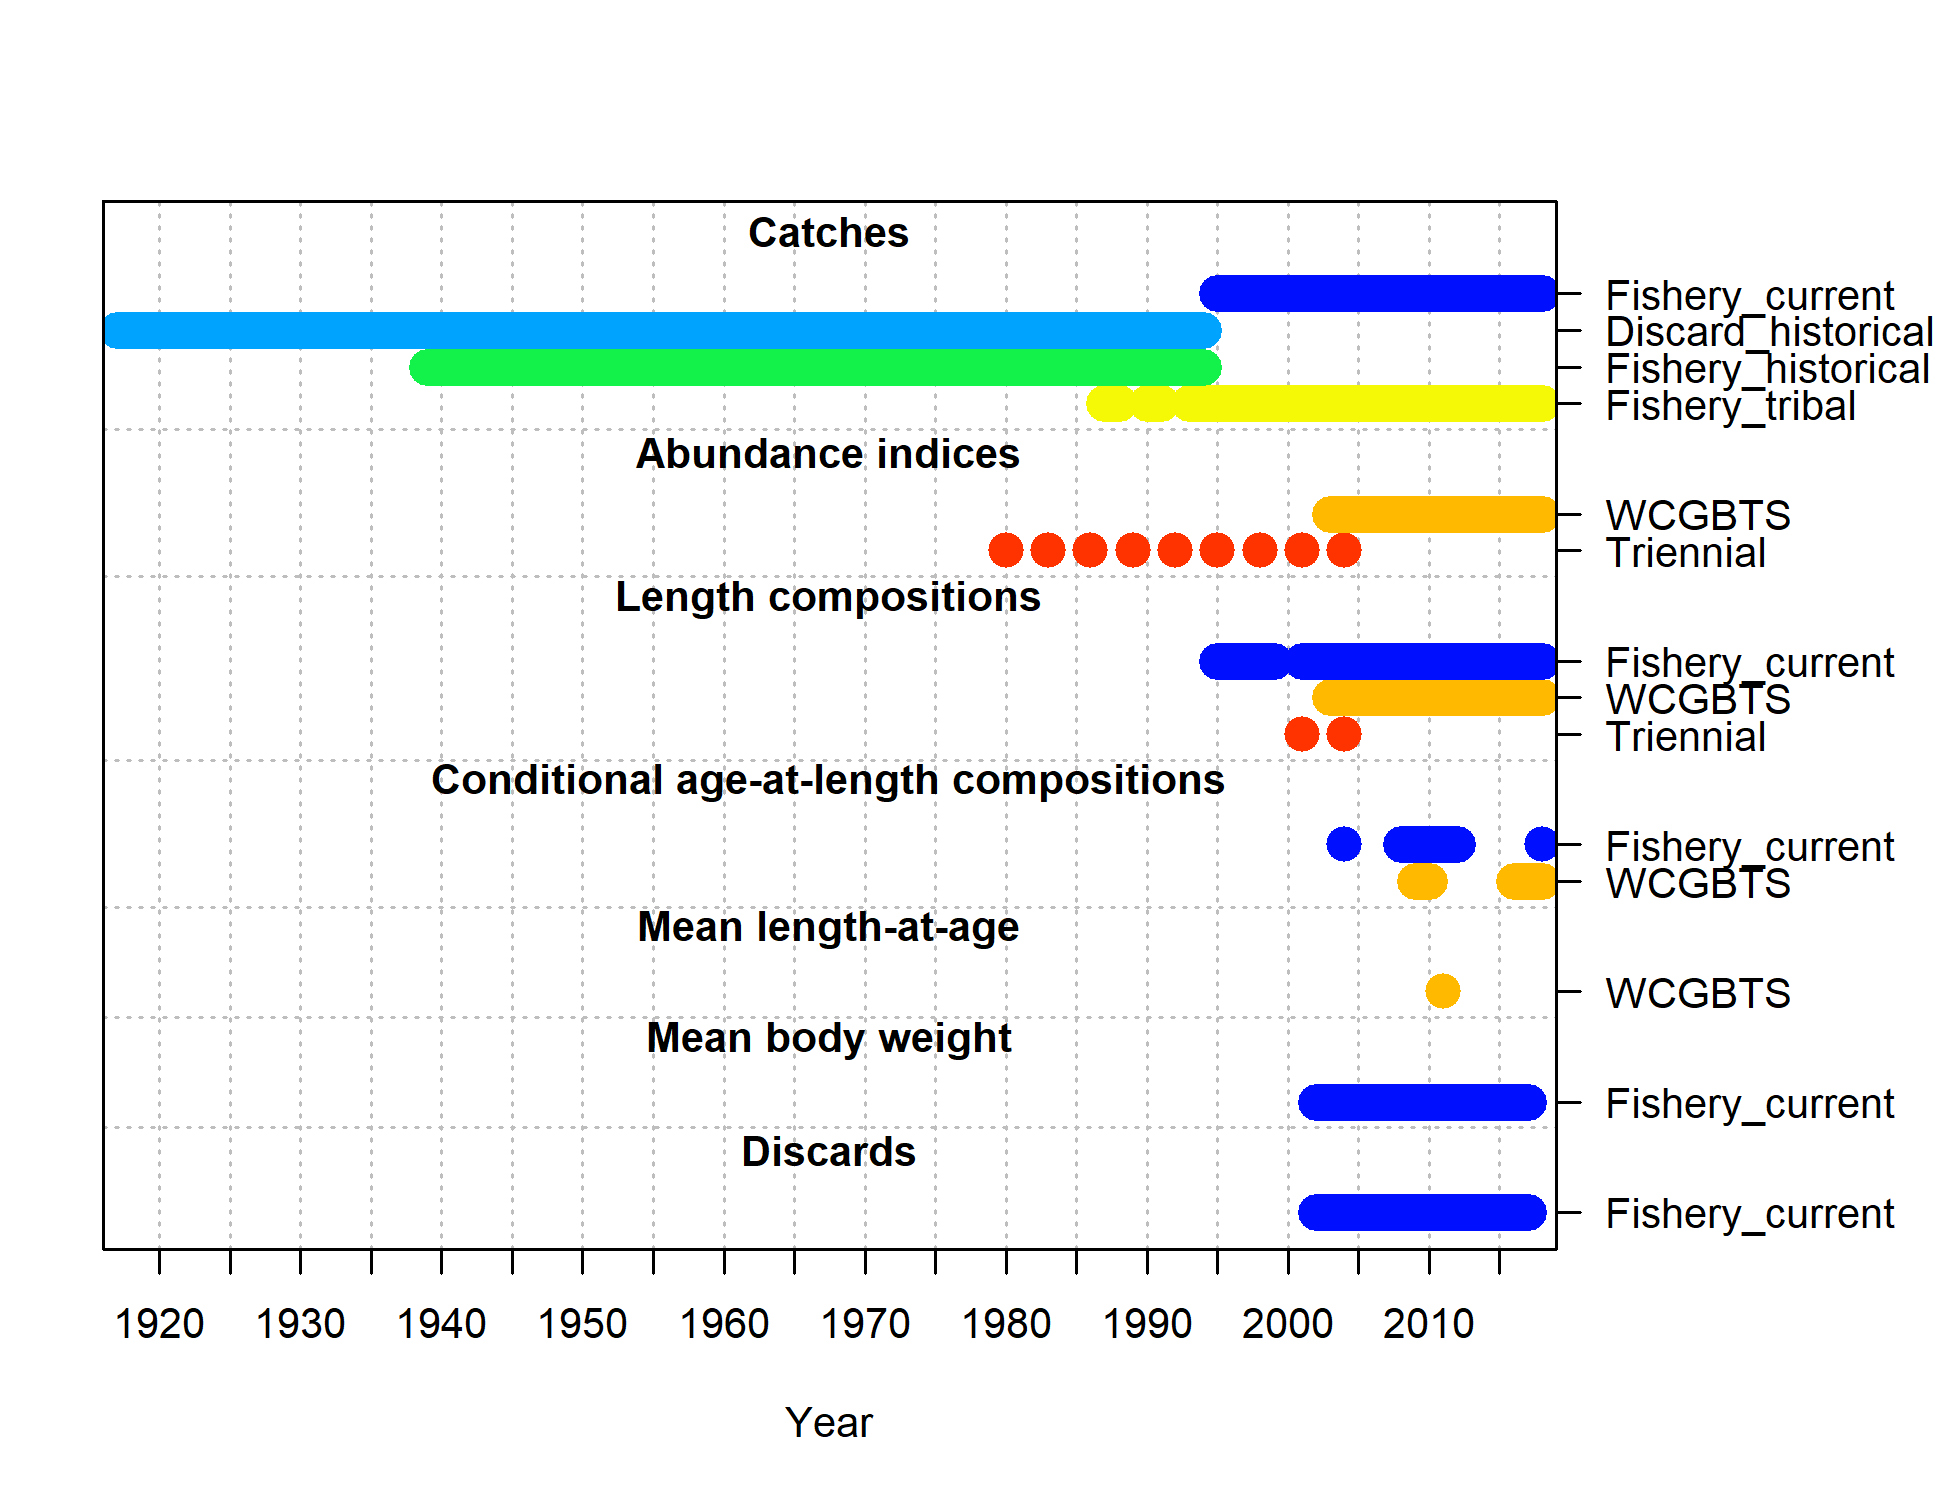
\includegraphics{r4ss/plots_mod1/data_plot.png}
\caption{Summary of data sources used in the model.}\label{fig:data_plot}
\end{centering}
\end{figure}

\newpage

\FloatBarrier

\newpage

\begin{figure}[H]
\begin{centering}
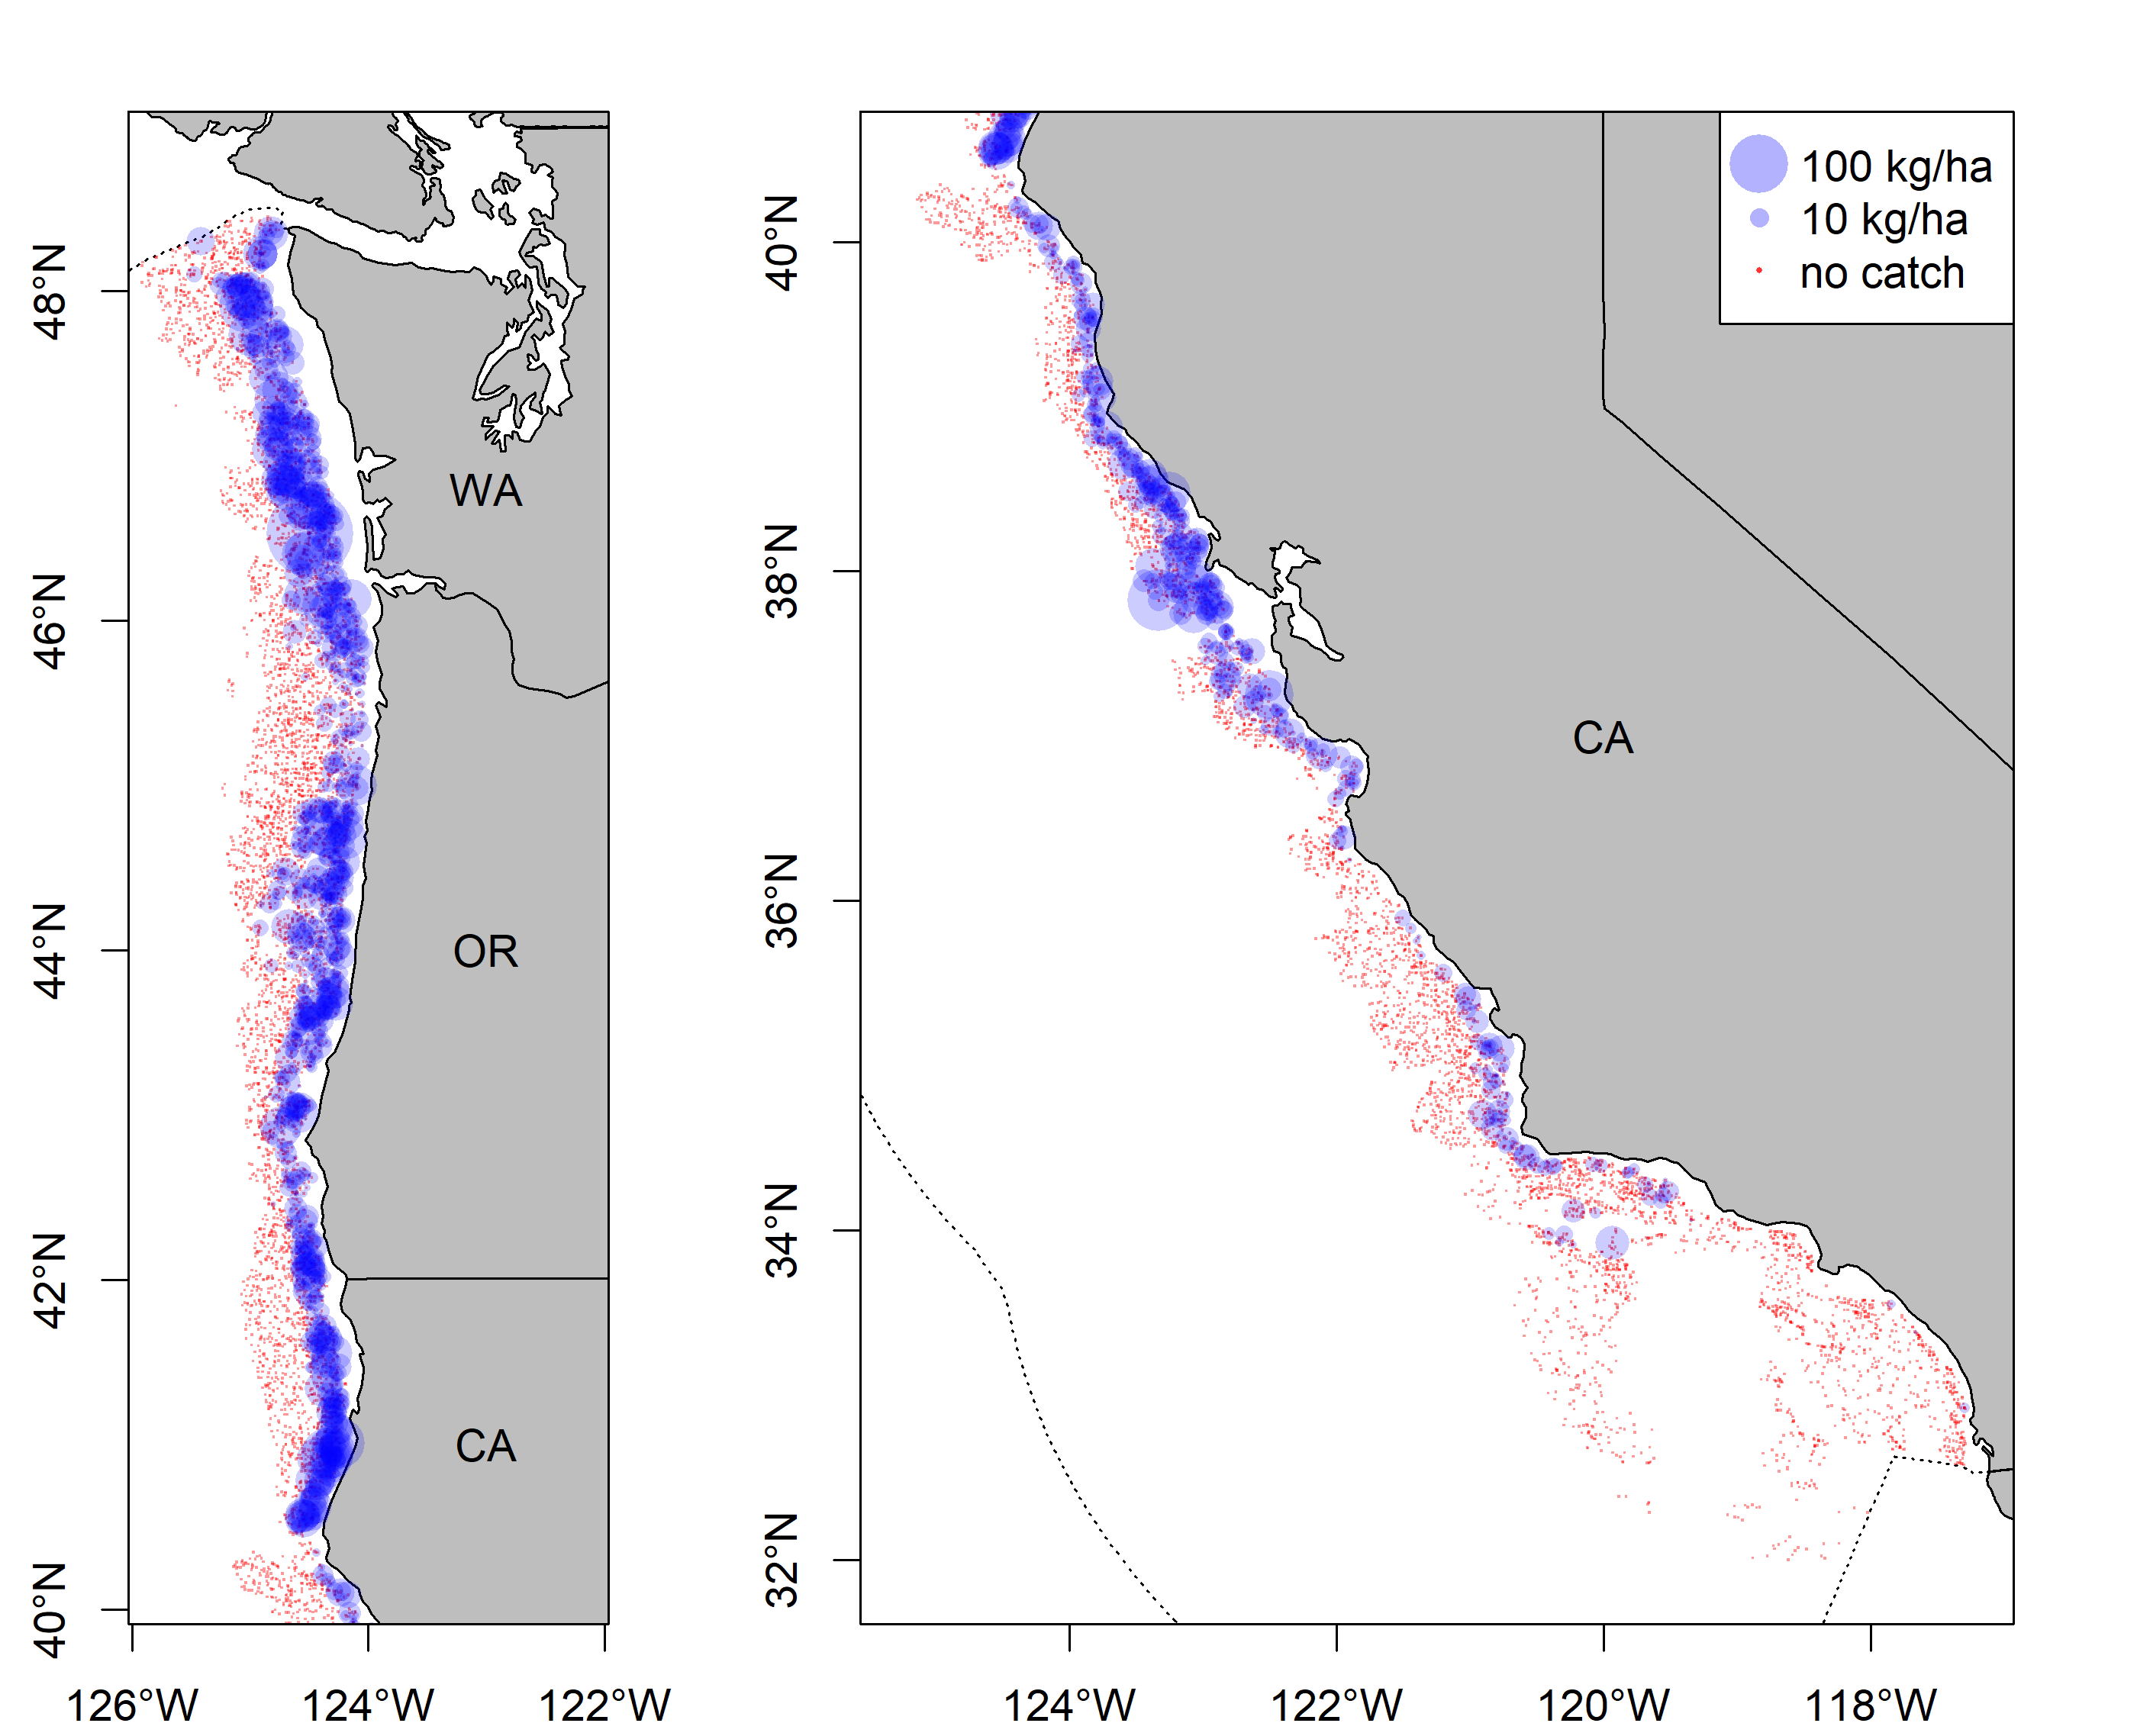
\includegraphics{Figures/survey_hauls_map.png}
\caption{Map showing the distribution of Big Skate within the area covered by the West Coast Groundfish Bottom Trawl Survey aggregated over the years 2003--2018.}\label{fig:survey_hauls_map}
\end{centering}
\end{figure}

\newpage

\FloatBarrier

\begin{figure}
\centering
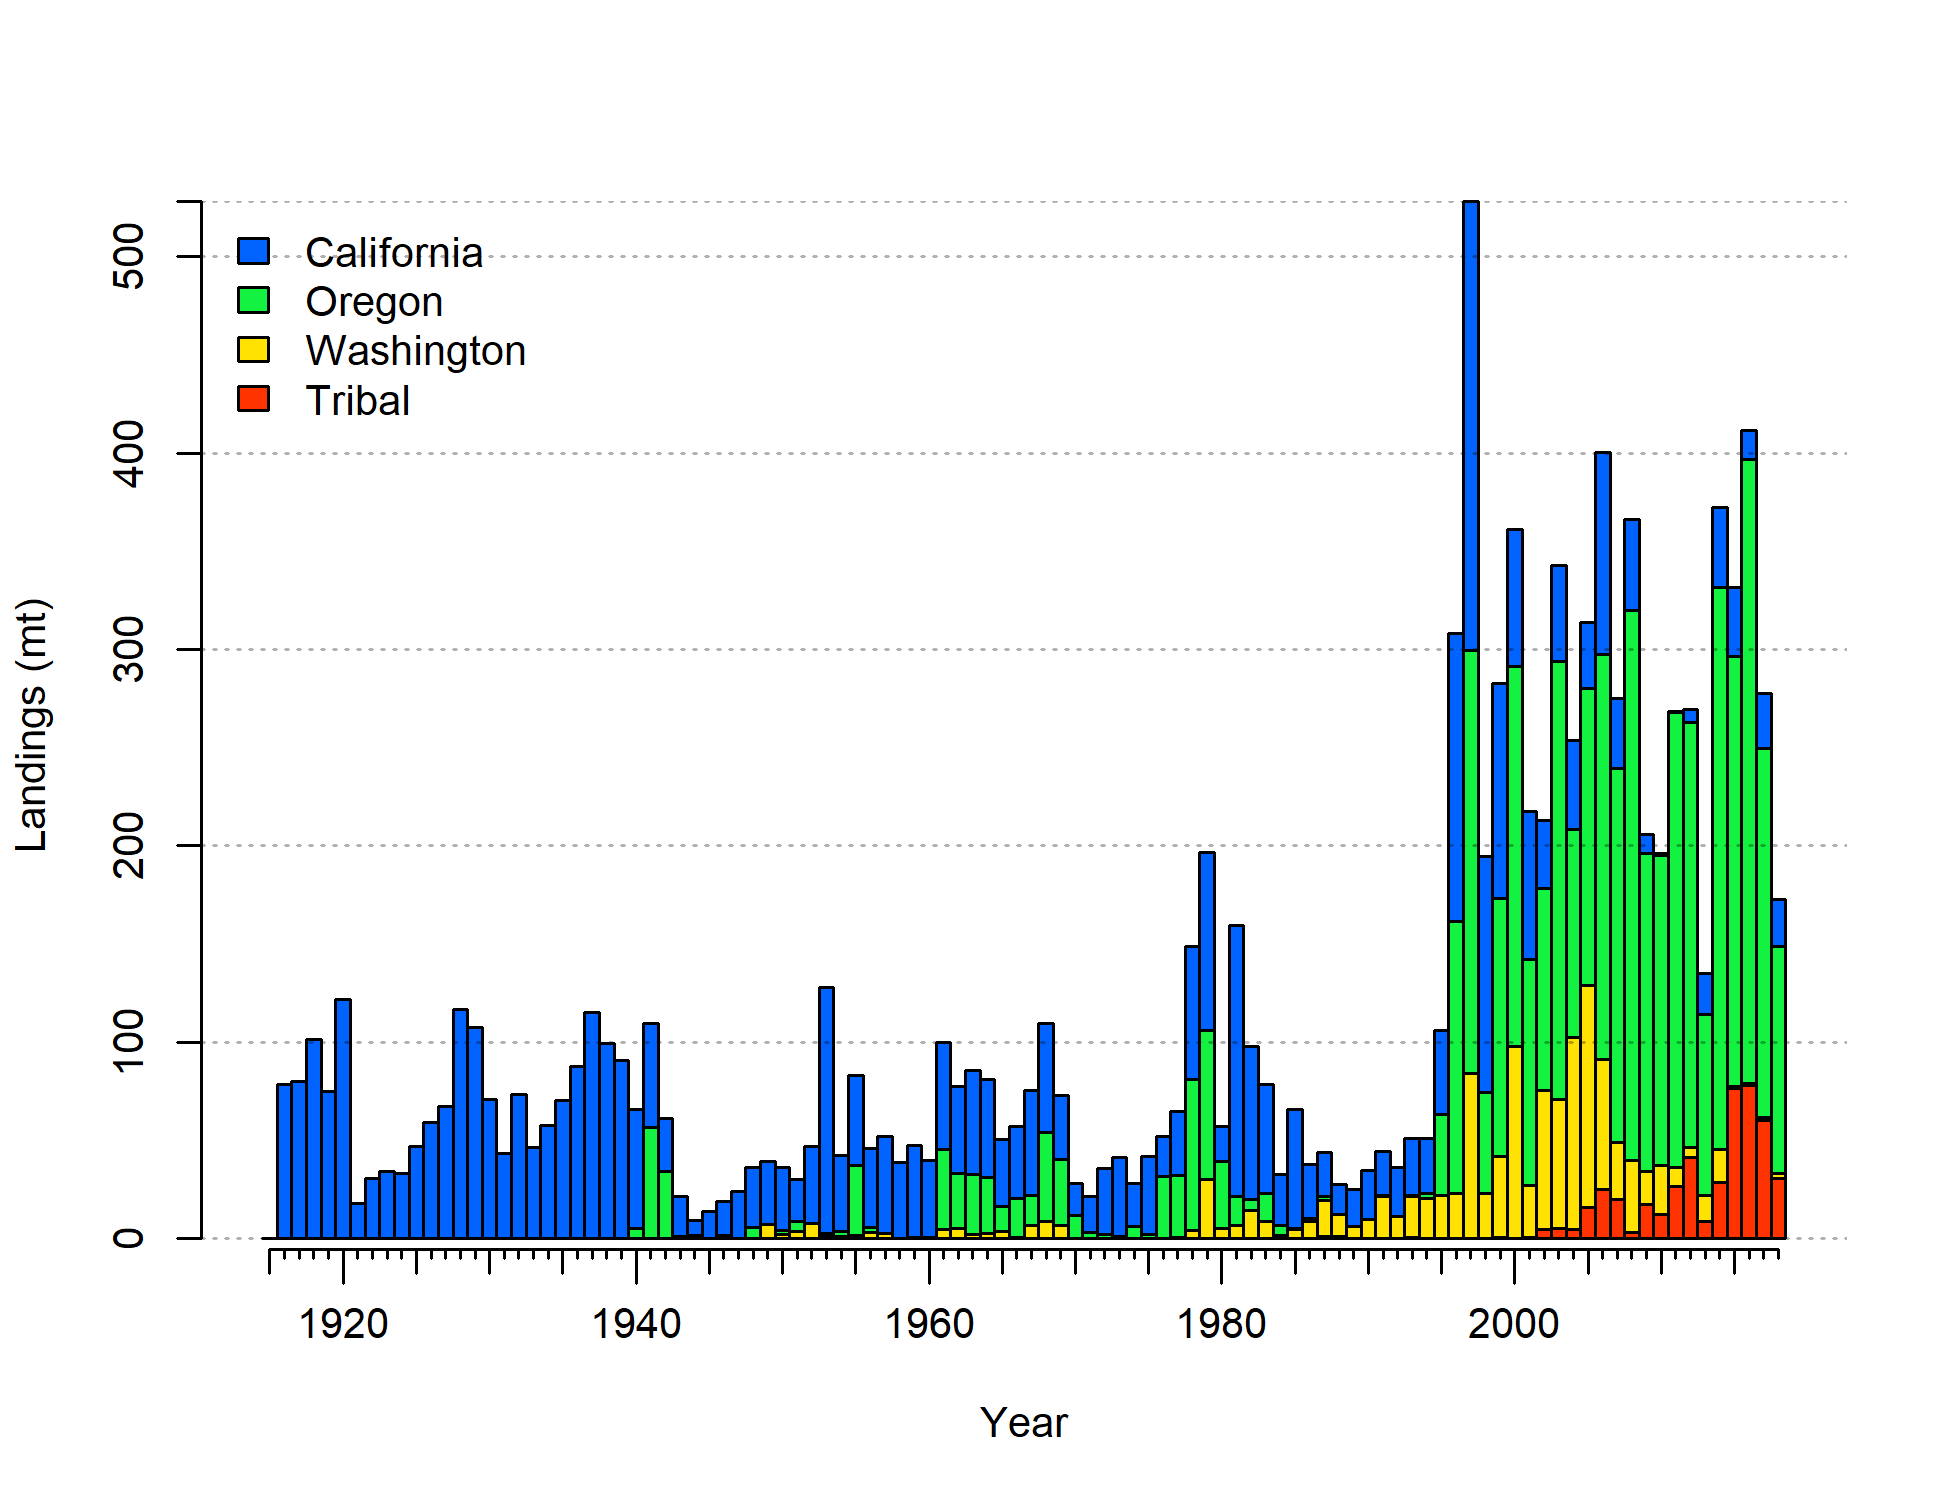
\includegraphics{Figures/catch_by_source.png}
\caption{Reconstructed landings by area. Tribal catch was all landed in
Washington. \label{fig:catch_by_state}}
\end{figure}

\begin{figure}
\centering
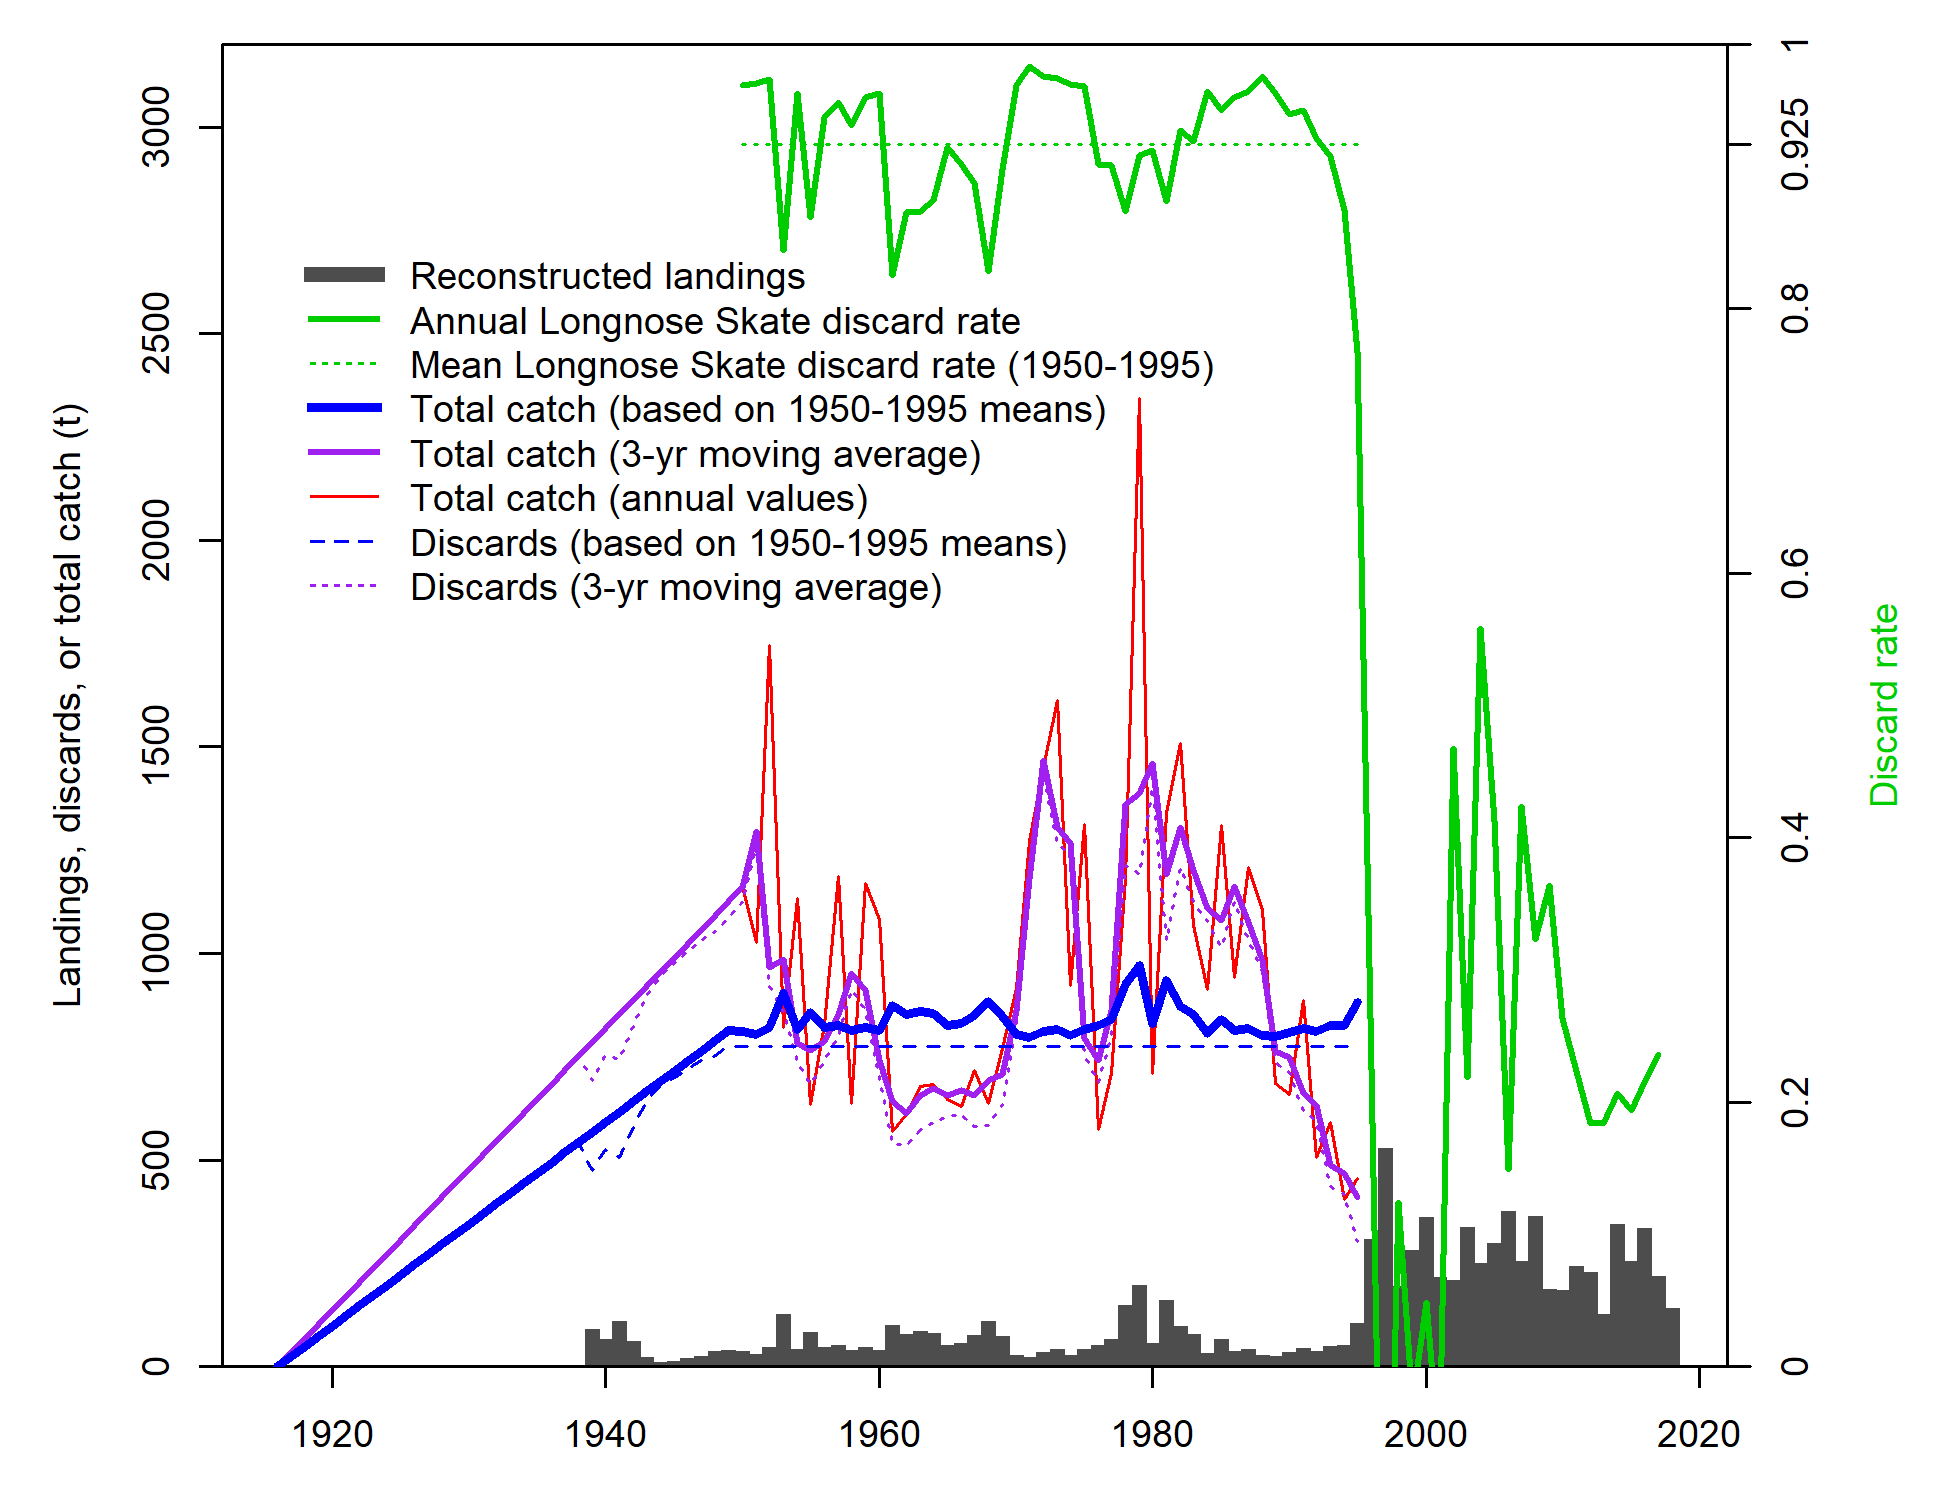
\includegraphics{Figures/discard_calculations.png}
\caption{Estimated total catch using different assumptions for discards.
The discard rates shown in green lines are relative to the right-hand
axis while all other values are relative to the left-hand
axis.\label{fig:discard_calculations}}
\end{figure}

\begin{figure}
\centering
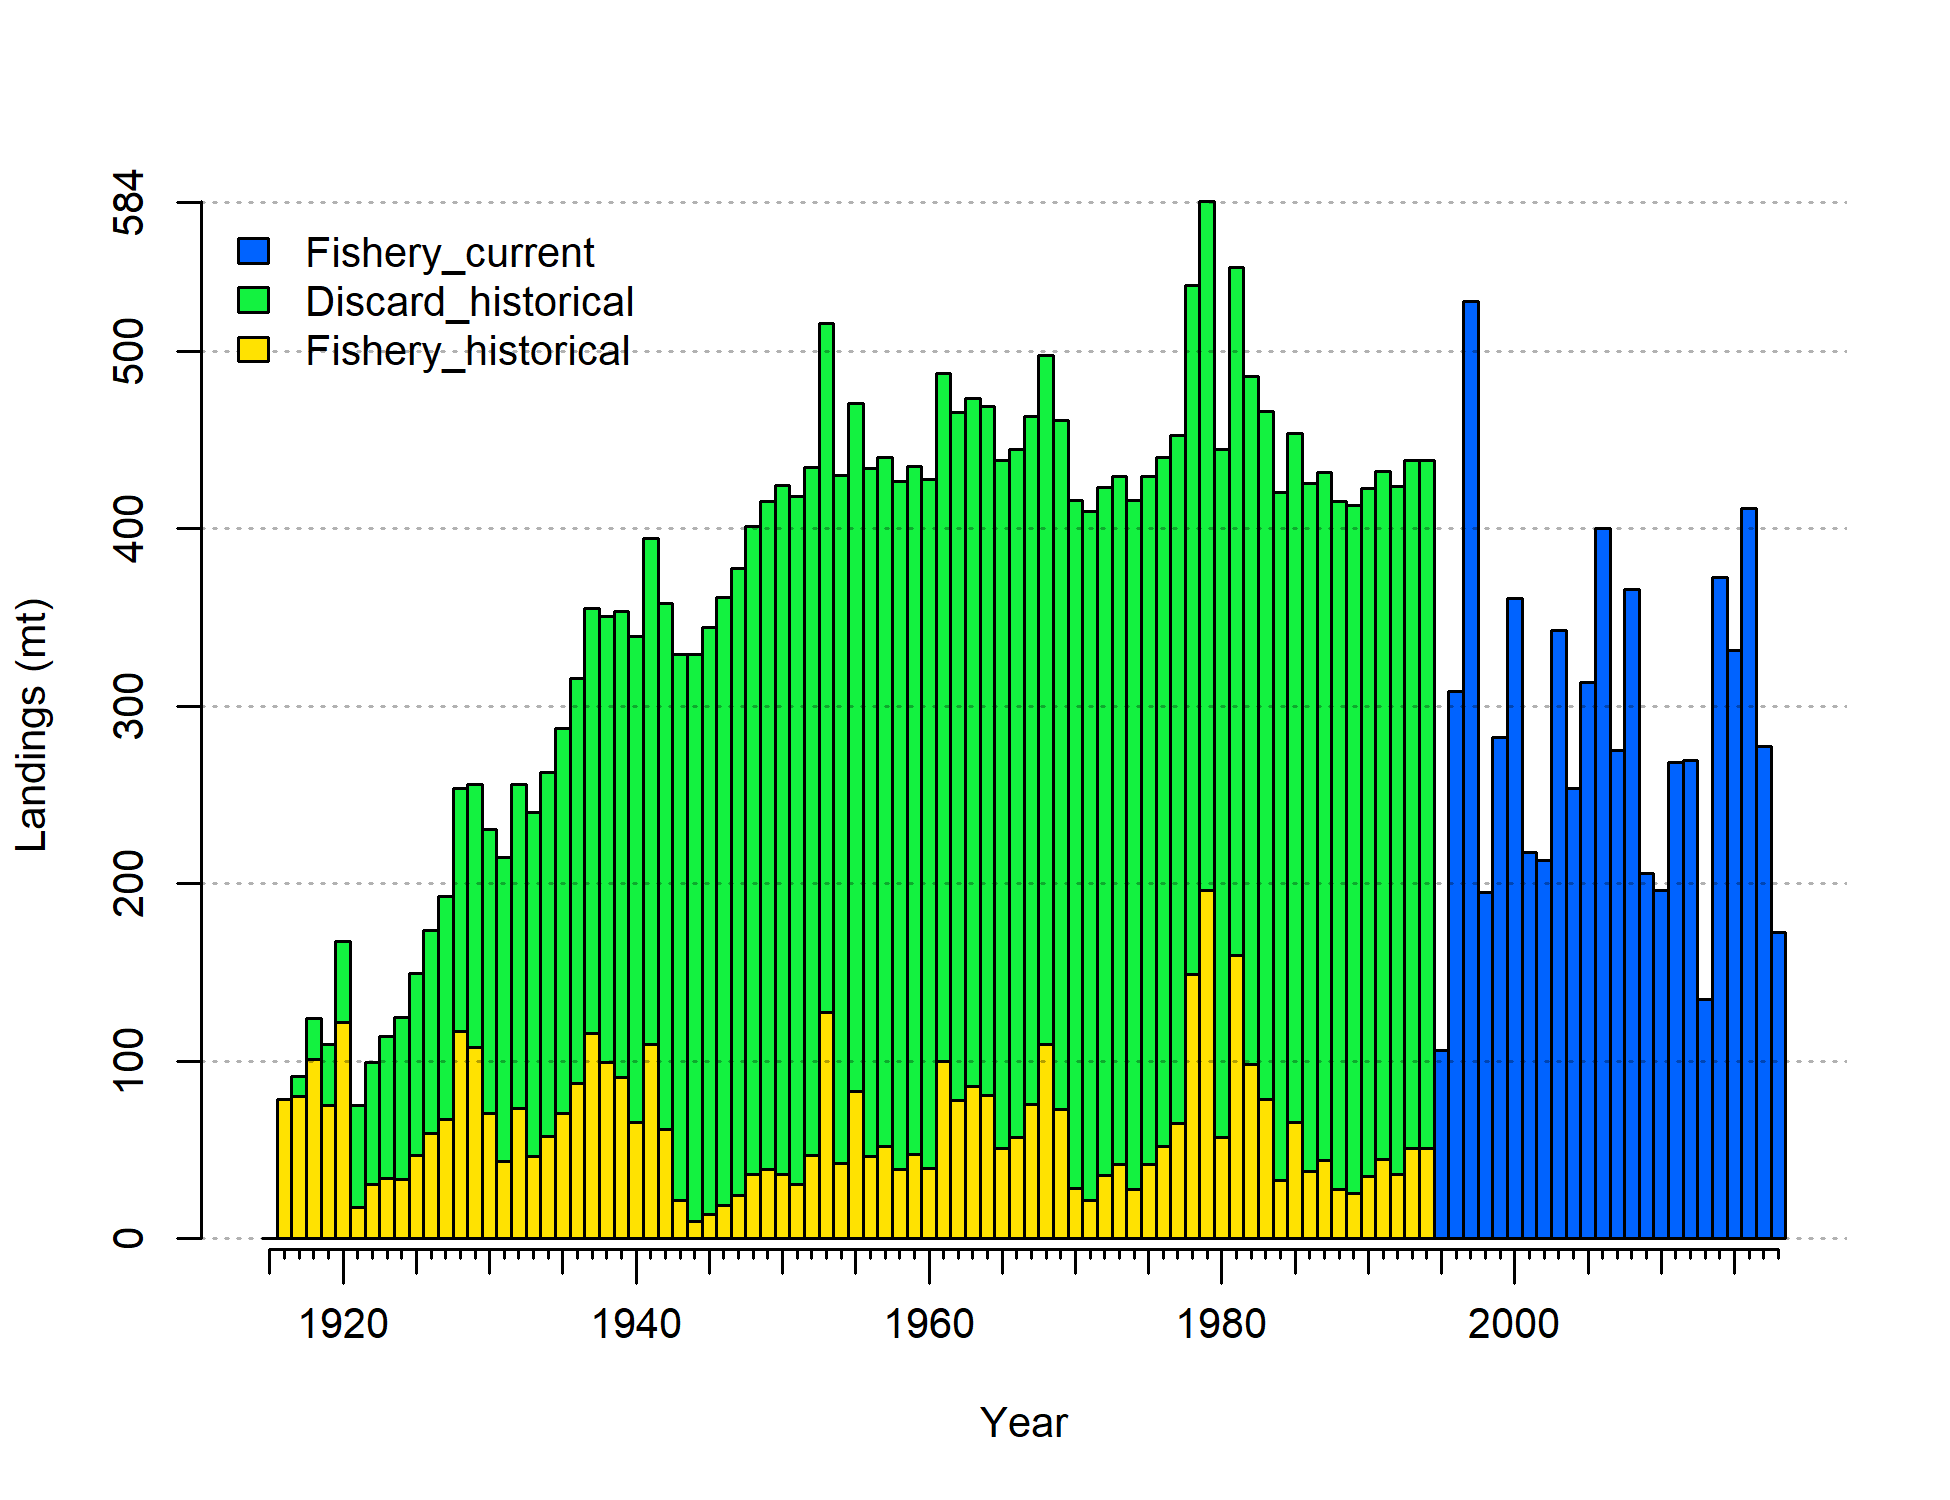
\includegraphics{r4ss/plots_mod1/catch2 landings stacked.png}
\caption{Catch data input to the model under assumed fleet structure.
The historical discards shown in green have been scaled to account for
an assumed 50\% discard mortality. Discards during the period from 1995
onward are not represented here as they are estimated within the model.
\label{fig:catch_input_plot}}
\end{figure}

\FloatBarrier

\begin{figure}
\centering
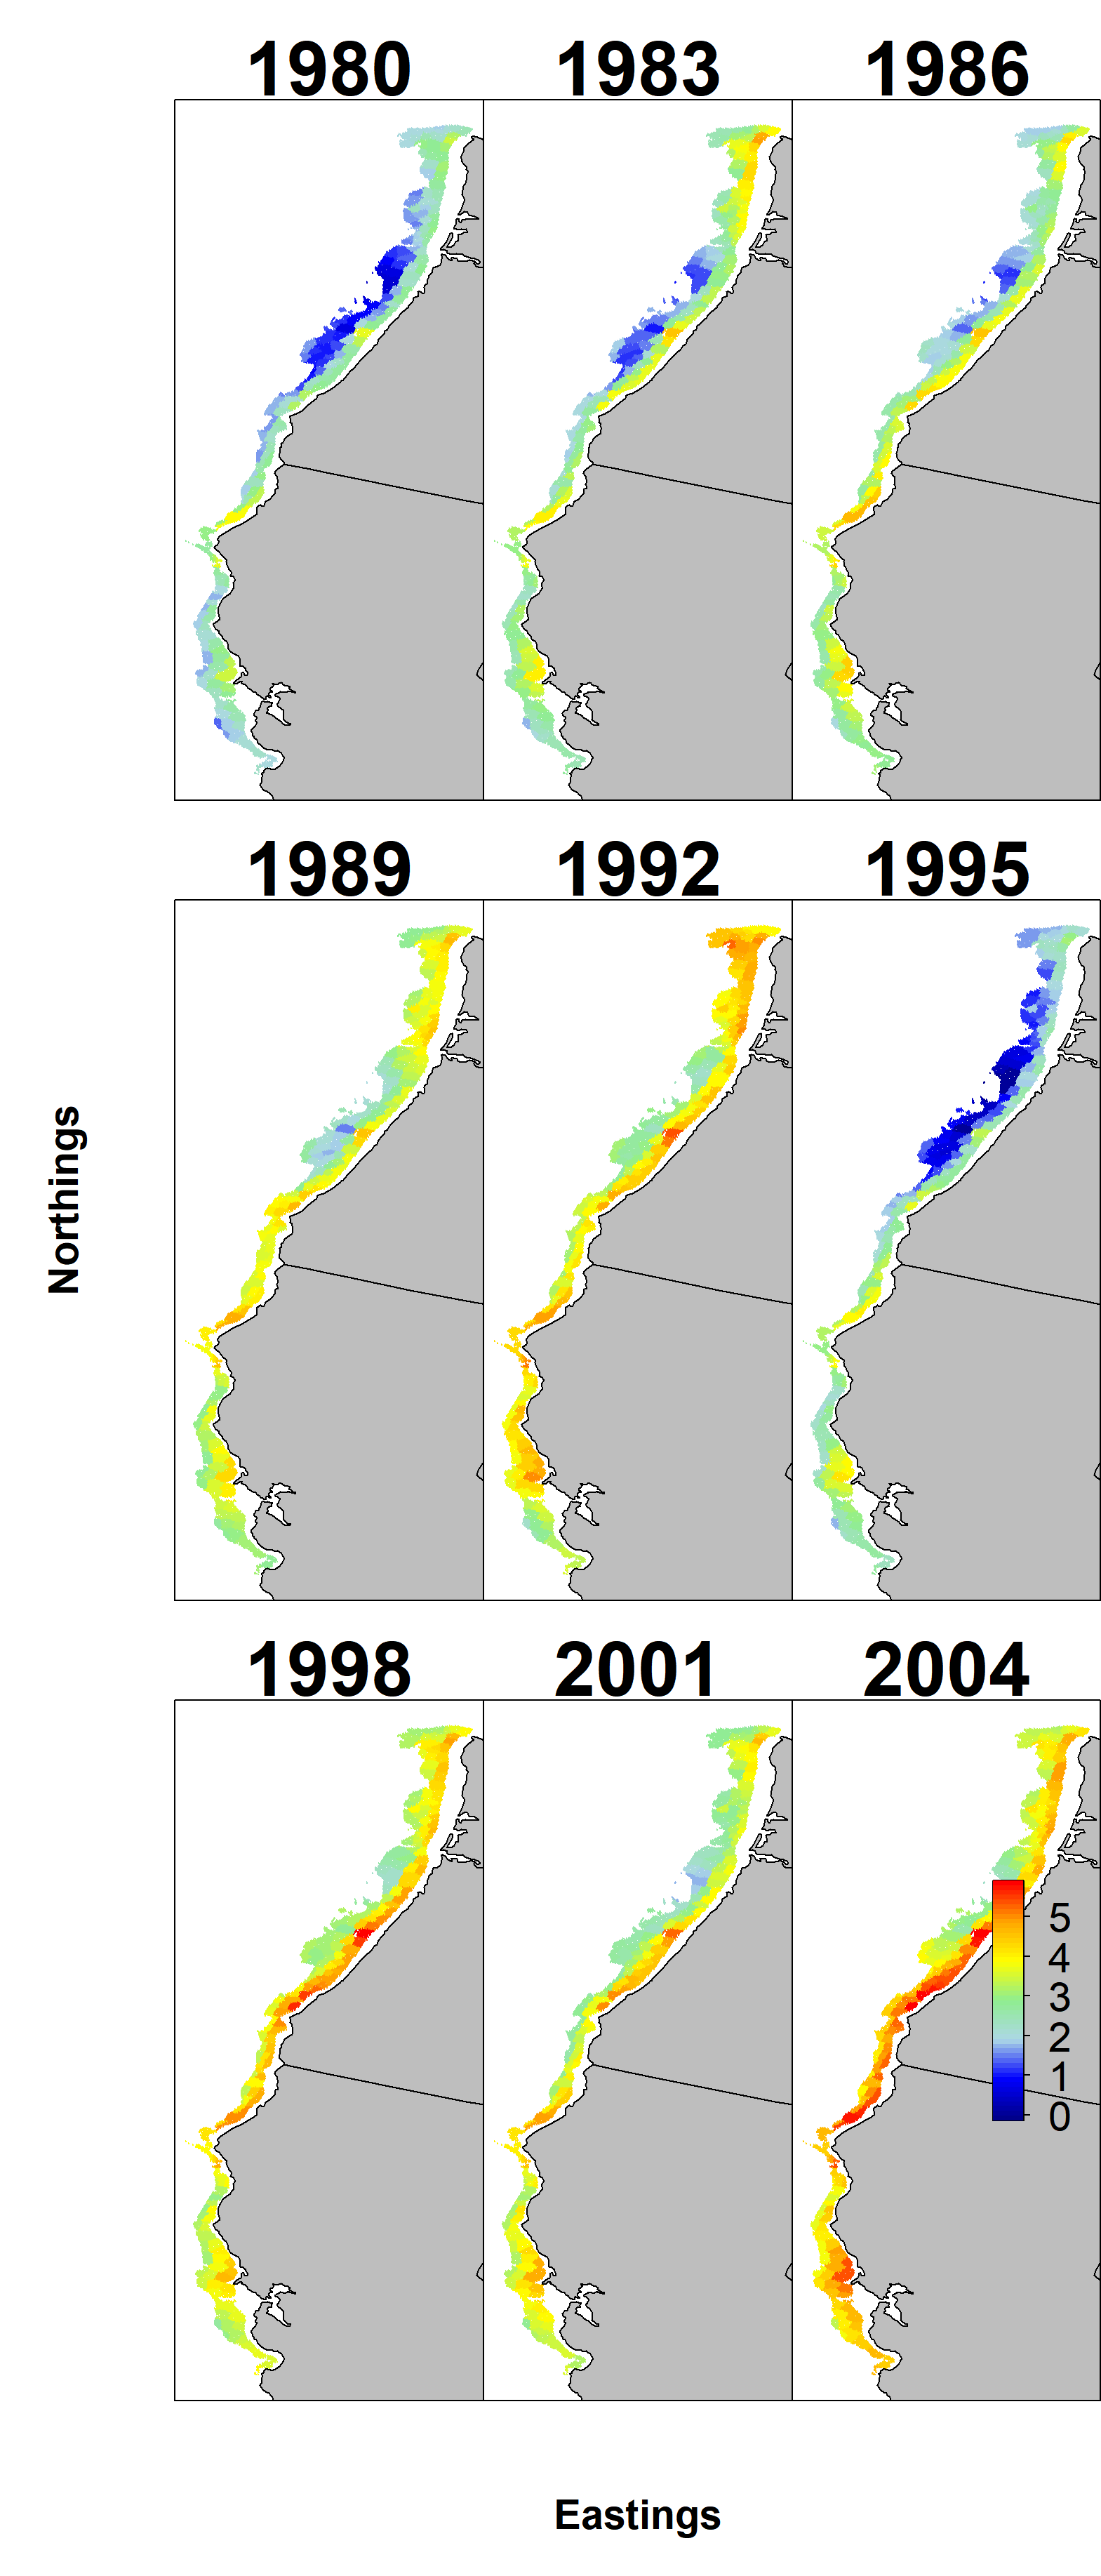
\includegraphics{Figures/VAST_Yearly_Dens_Triennial.png}
\caption{Map of estimated density by year for Big Skate in the Triennial
survey. \label{fig:VAST_Yearly_Dens_Triennial}}
\end{figure}

\begin{figure}
\centering
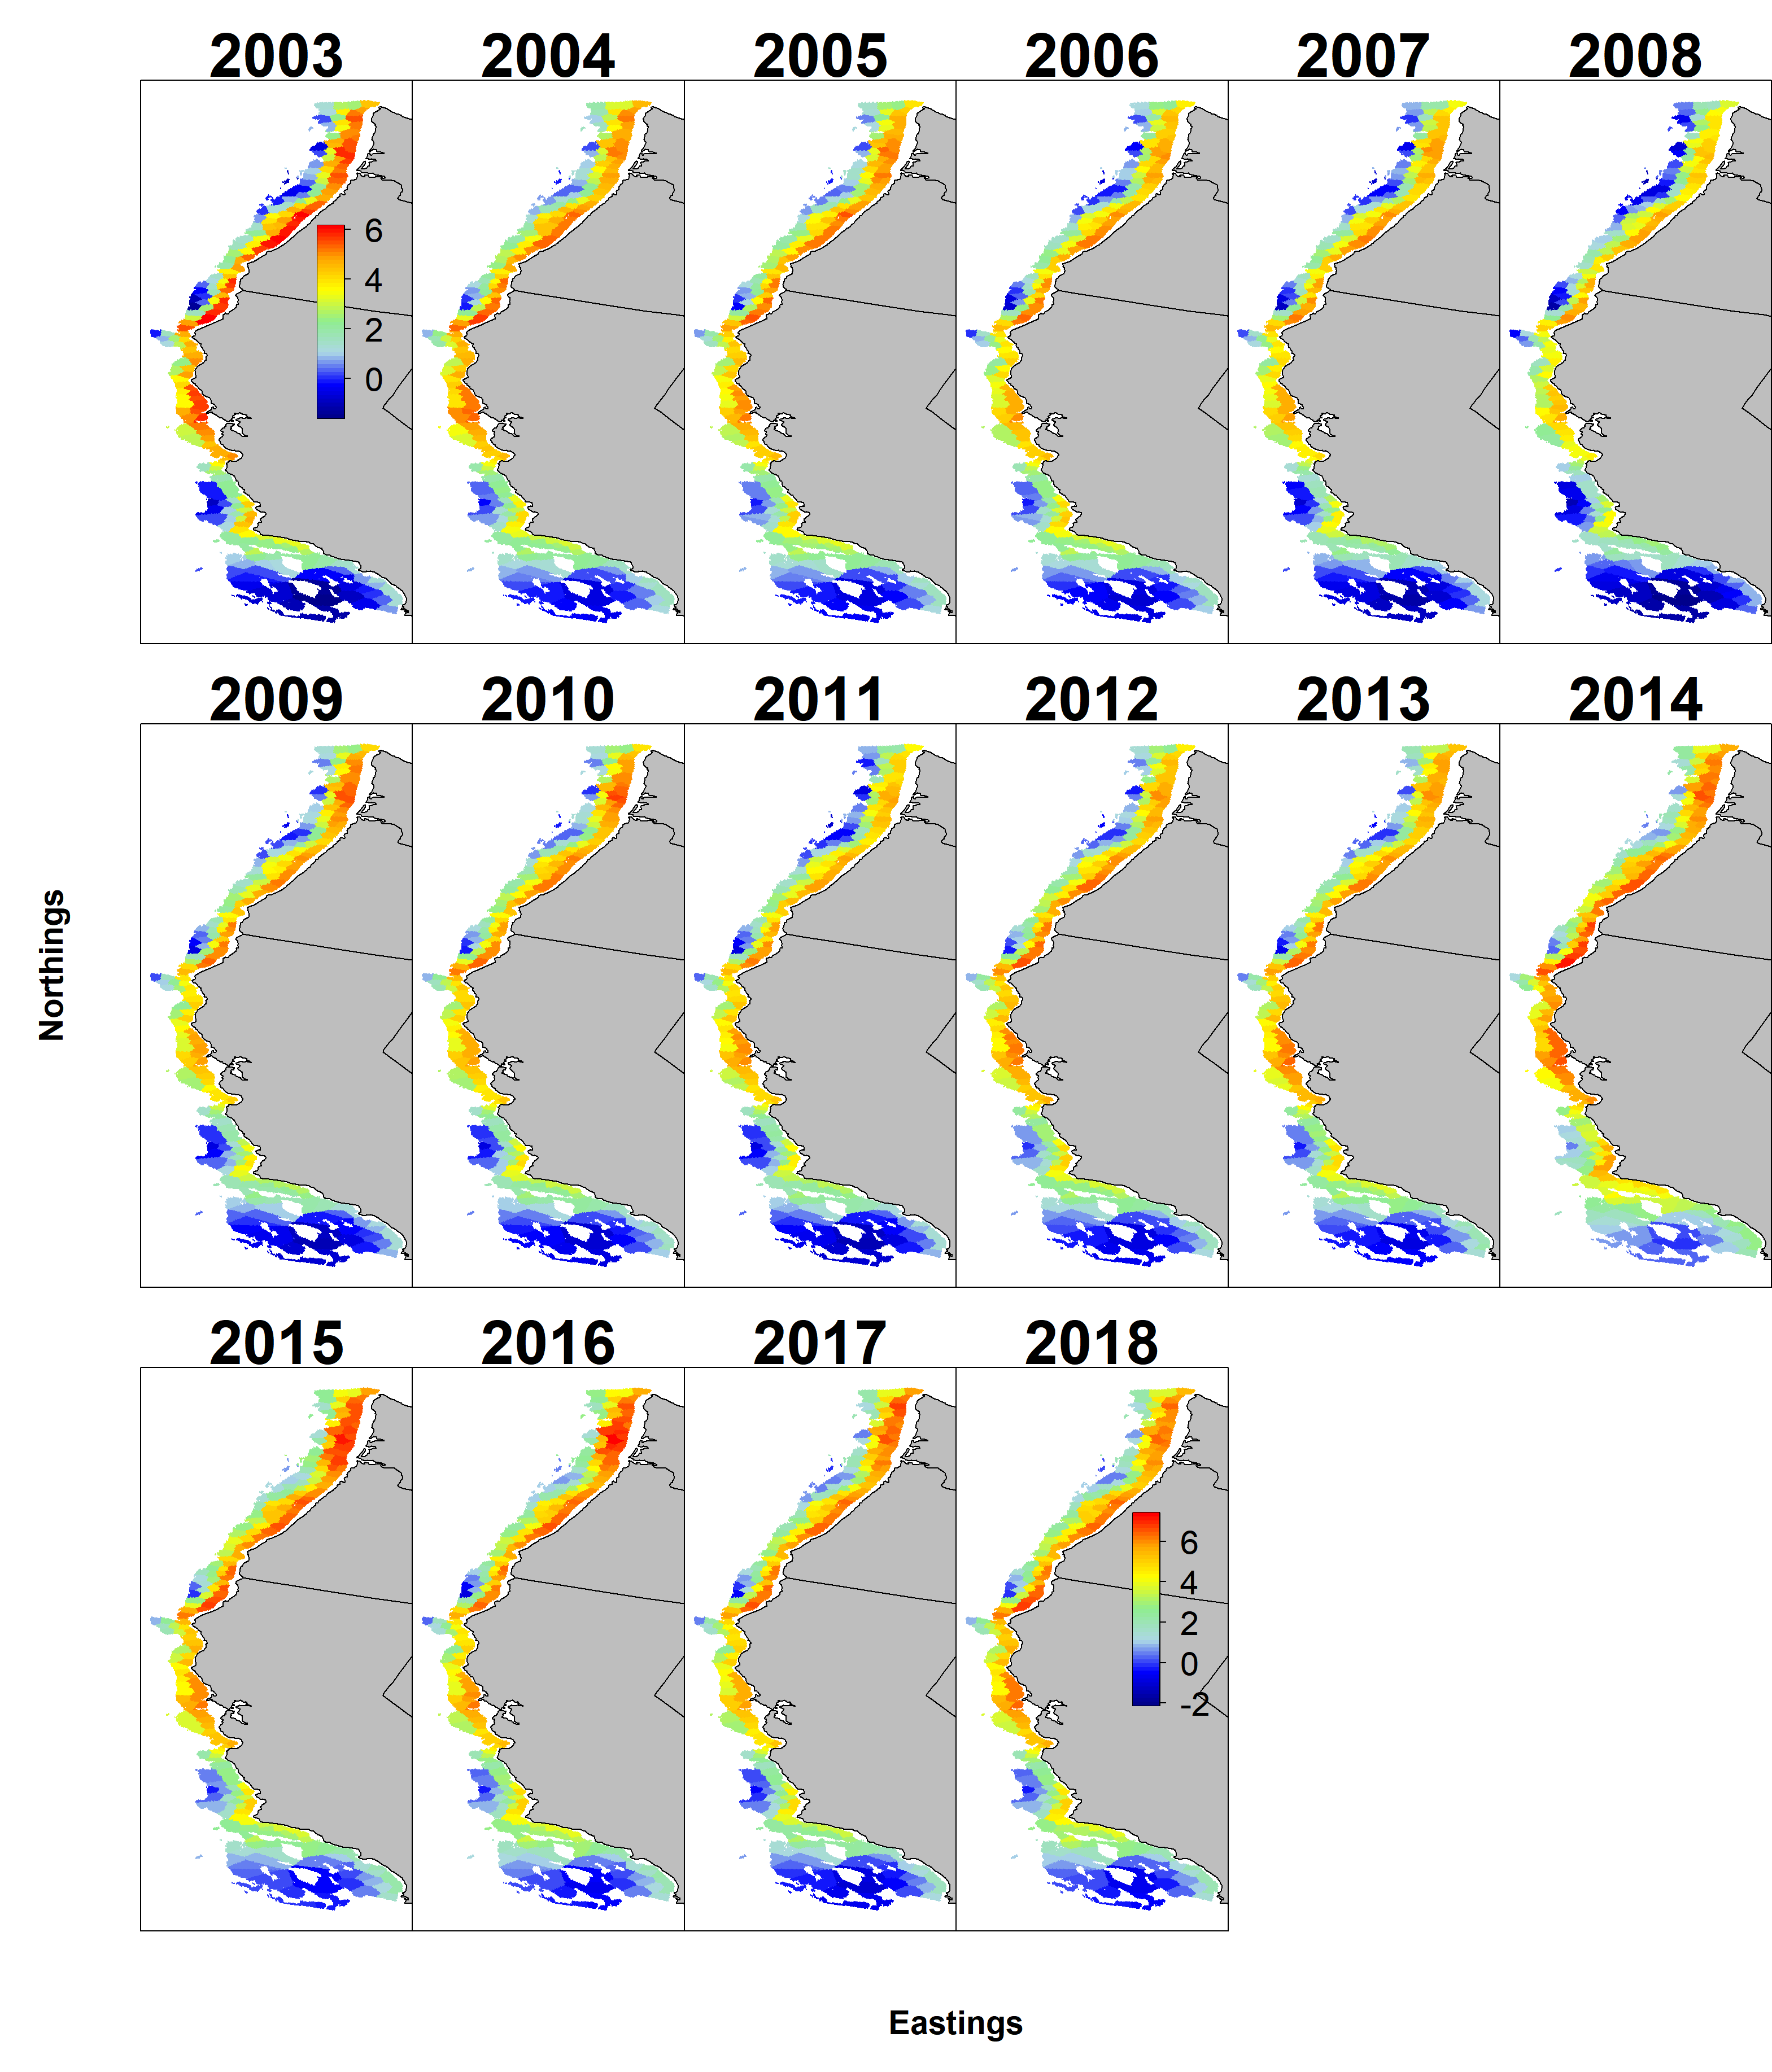
\includegraphics{Figures/VAST_Yearly_Dens_WCGBTS.png}
\caption{Map of estimated density by year for Big Skate in the WCGBT
Survey. \label{fig:VAST_Yearly_Dens_Triennial}}
\end{figure}

\begin{figure}
\centering
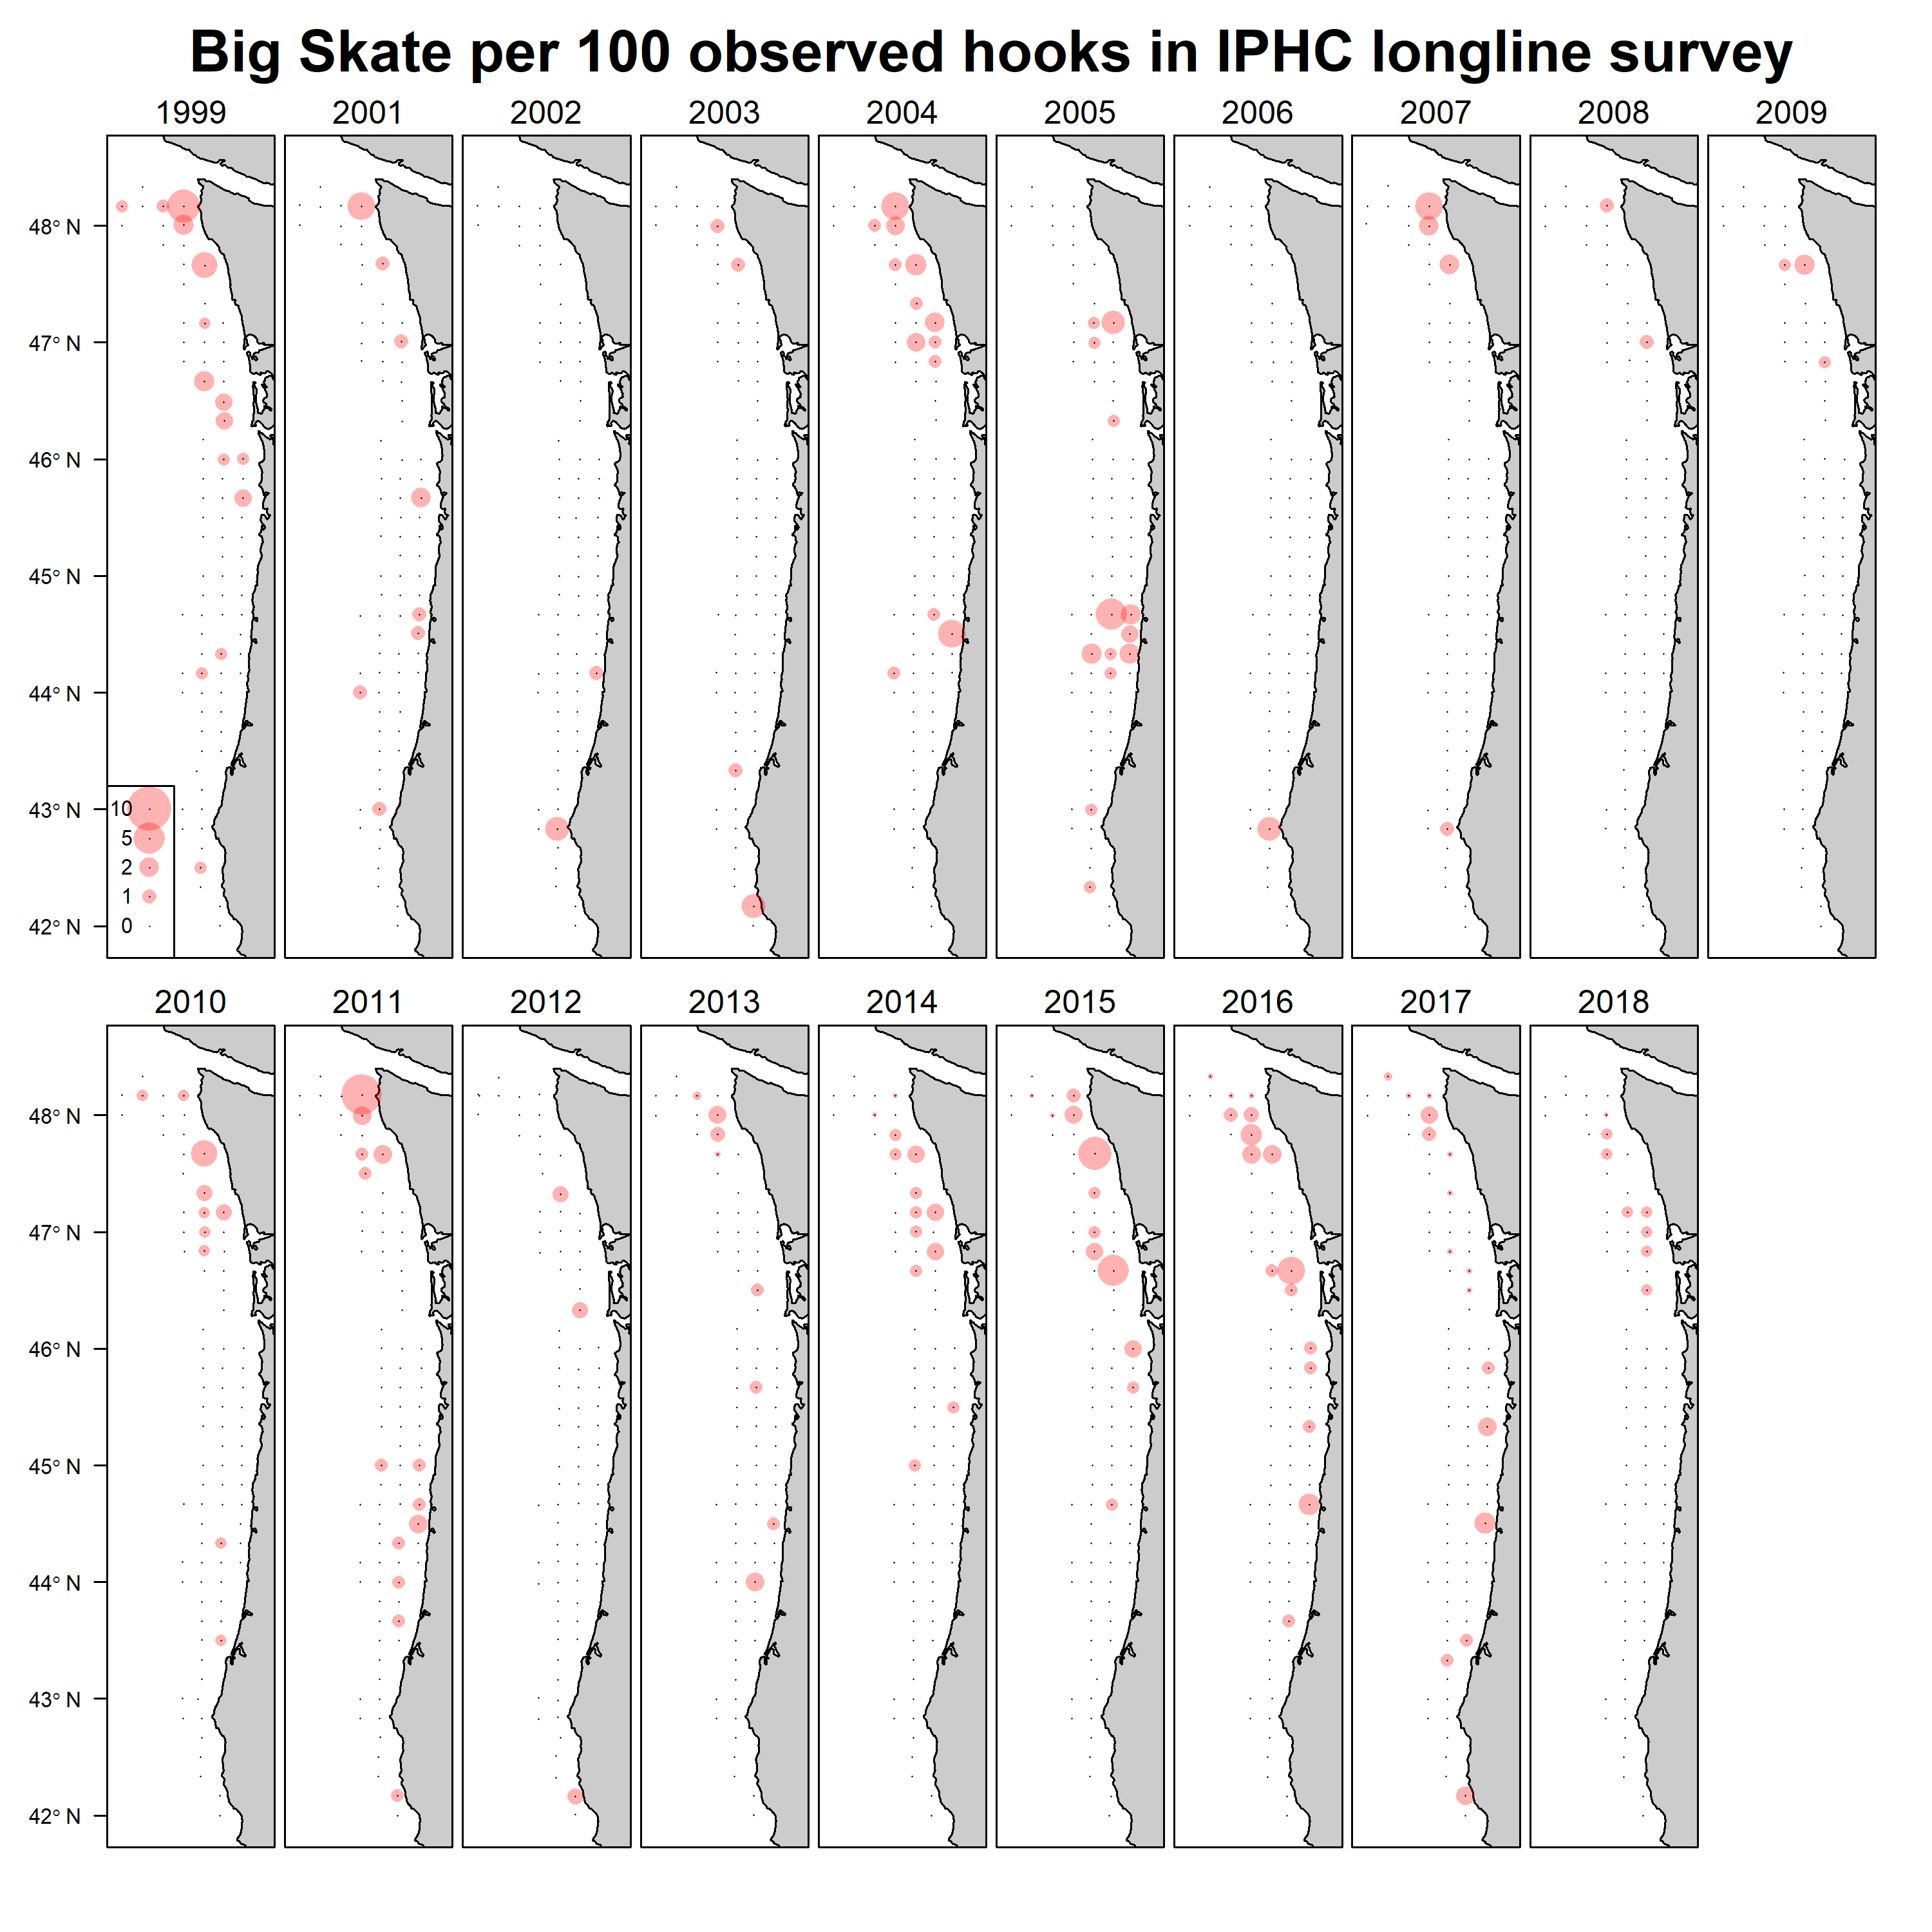
\includegraphics{Figures/IPHC_BigSkate_map.png}
\caption{Map of catch rates by year for Big Skate in the International
Pacific Halibut Commission longline survey. \label{fig:IPHC_map}}
\end{figure}

\FloatBarrier

\FloatBarrier

\FloatBarrier

\FloatBarrier

\FloatBarrier

\FloatBarrier

\newpage

\FloatBarrier

\newpage

\hypertarget{biology-figures}{%
\subsection{Biology Figures}\label{biology-figures}}

\FloatBarrier

\begin{figure}[H]
\begin{centering}
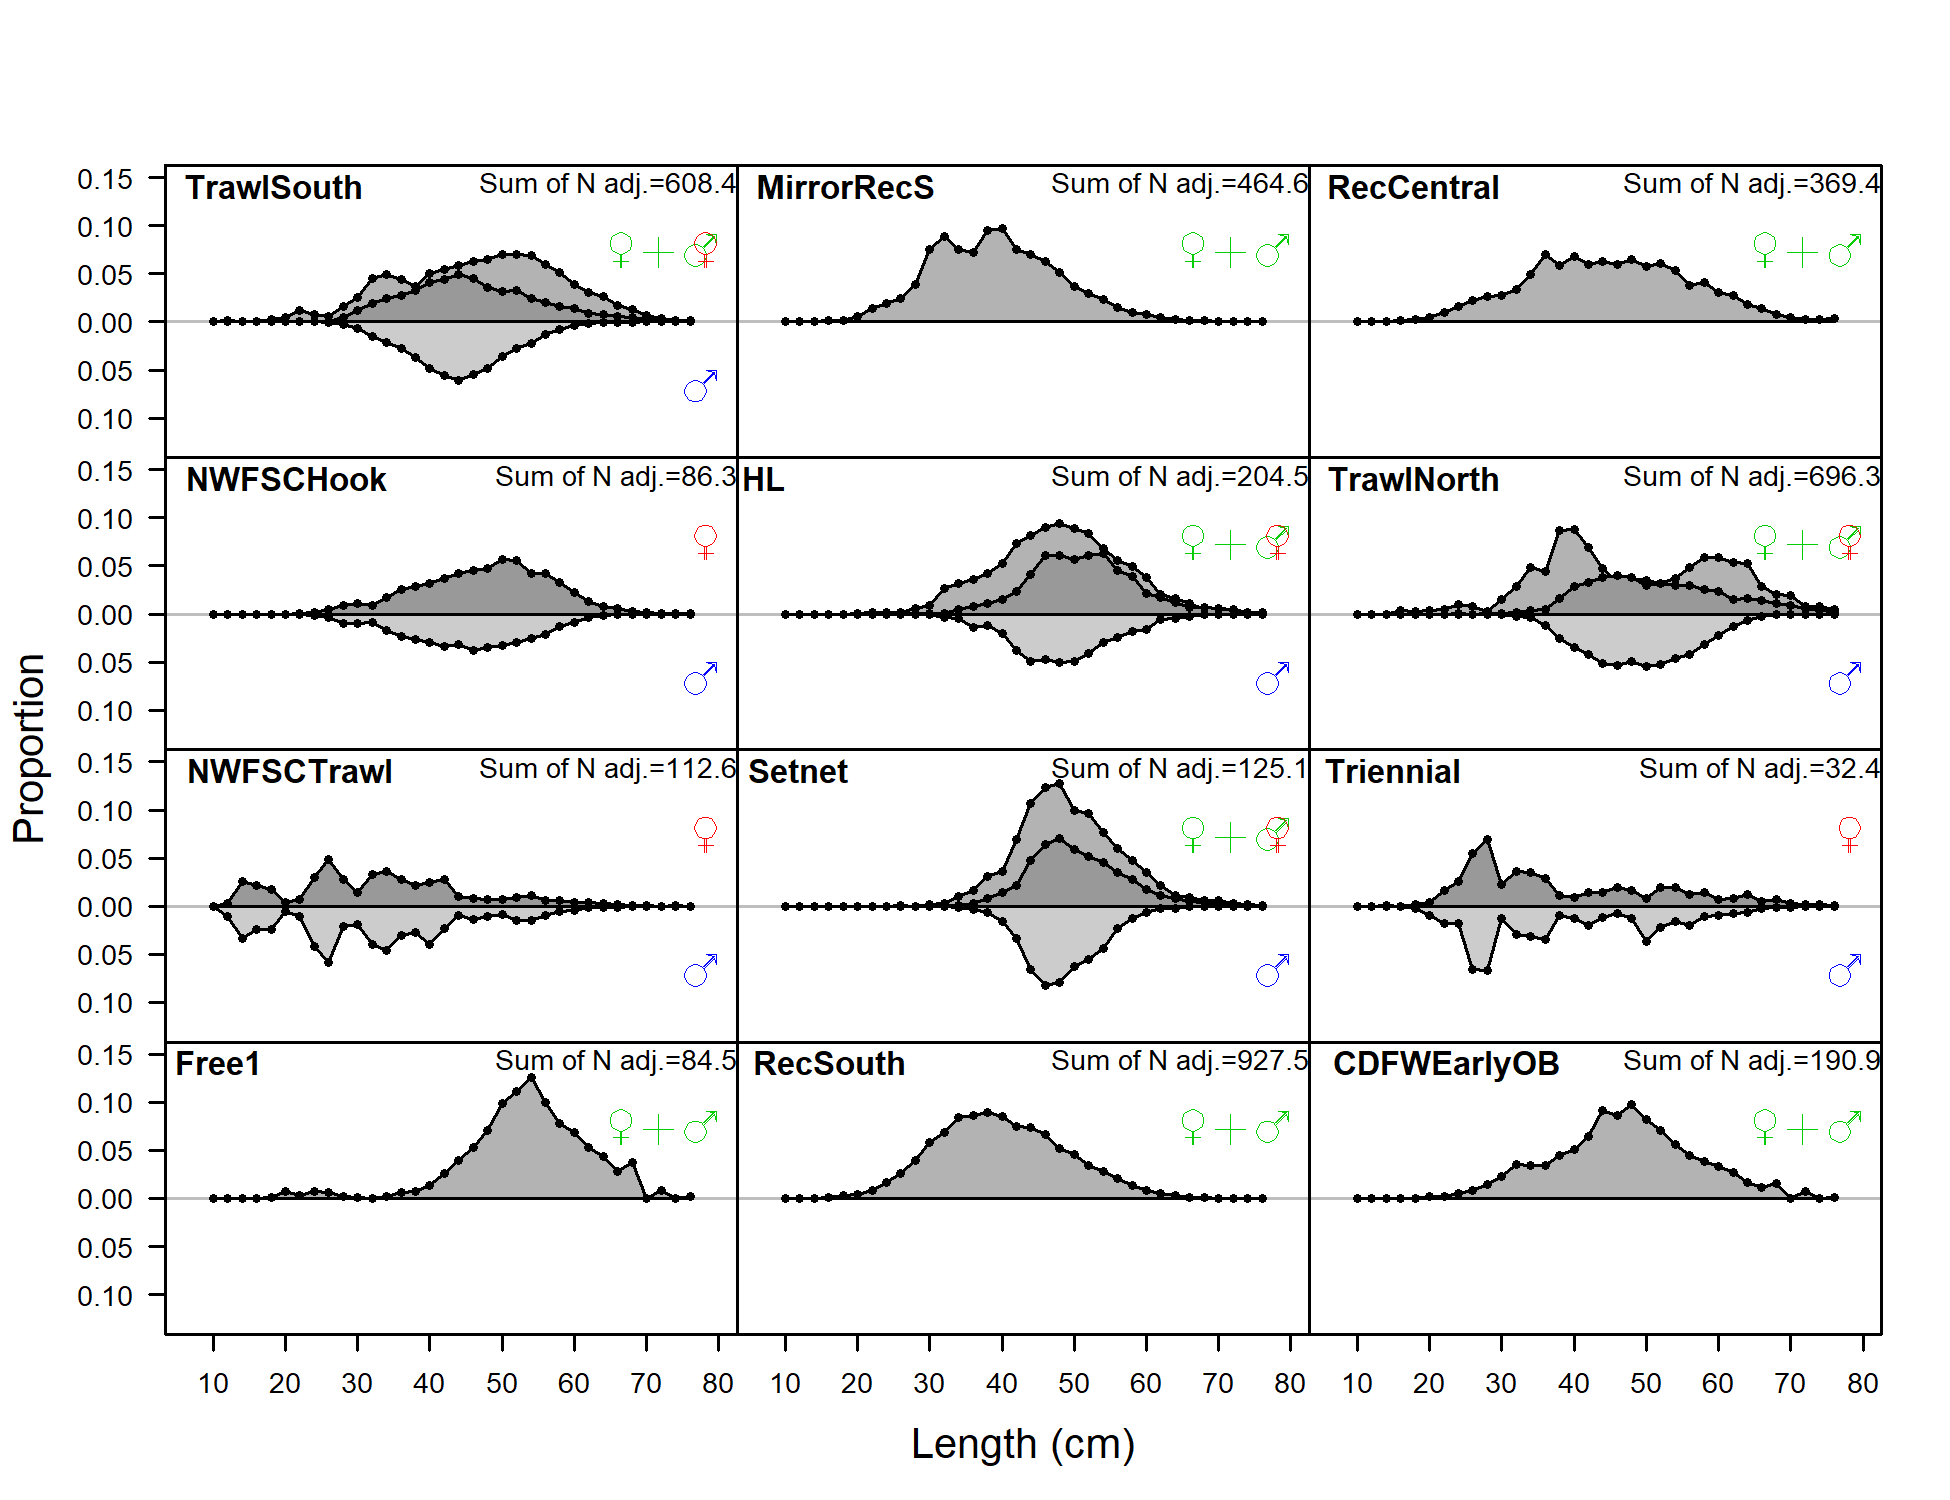
\includegraphics{r4ss/plots_mod1/comp_lendat__aggregated_across_time.png}
\caption{Length comp data, aggregated across time by fleet.}\label{fig:comp_lendat_aggregated_across_time}
\end{centering}
\end{figure}

\FloatBarrier

\begin{figure}
\centering
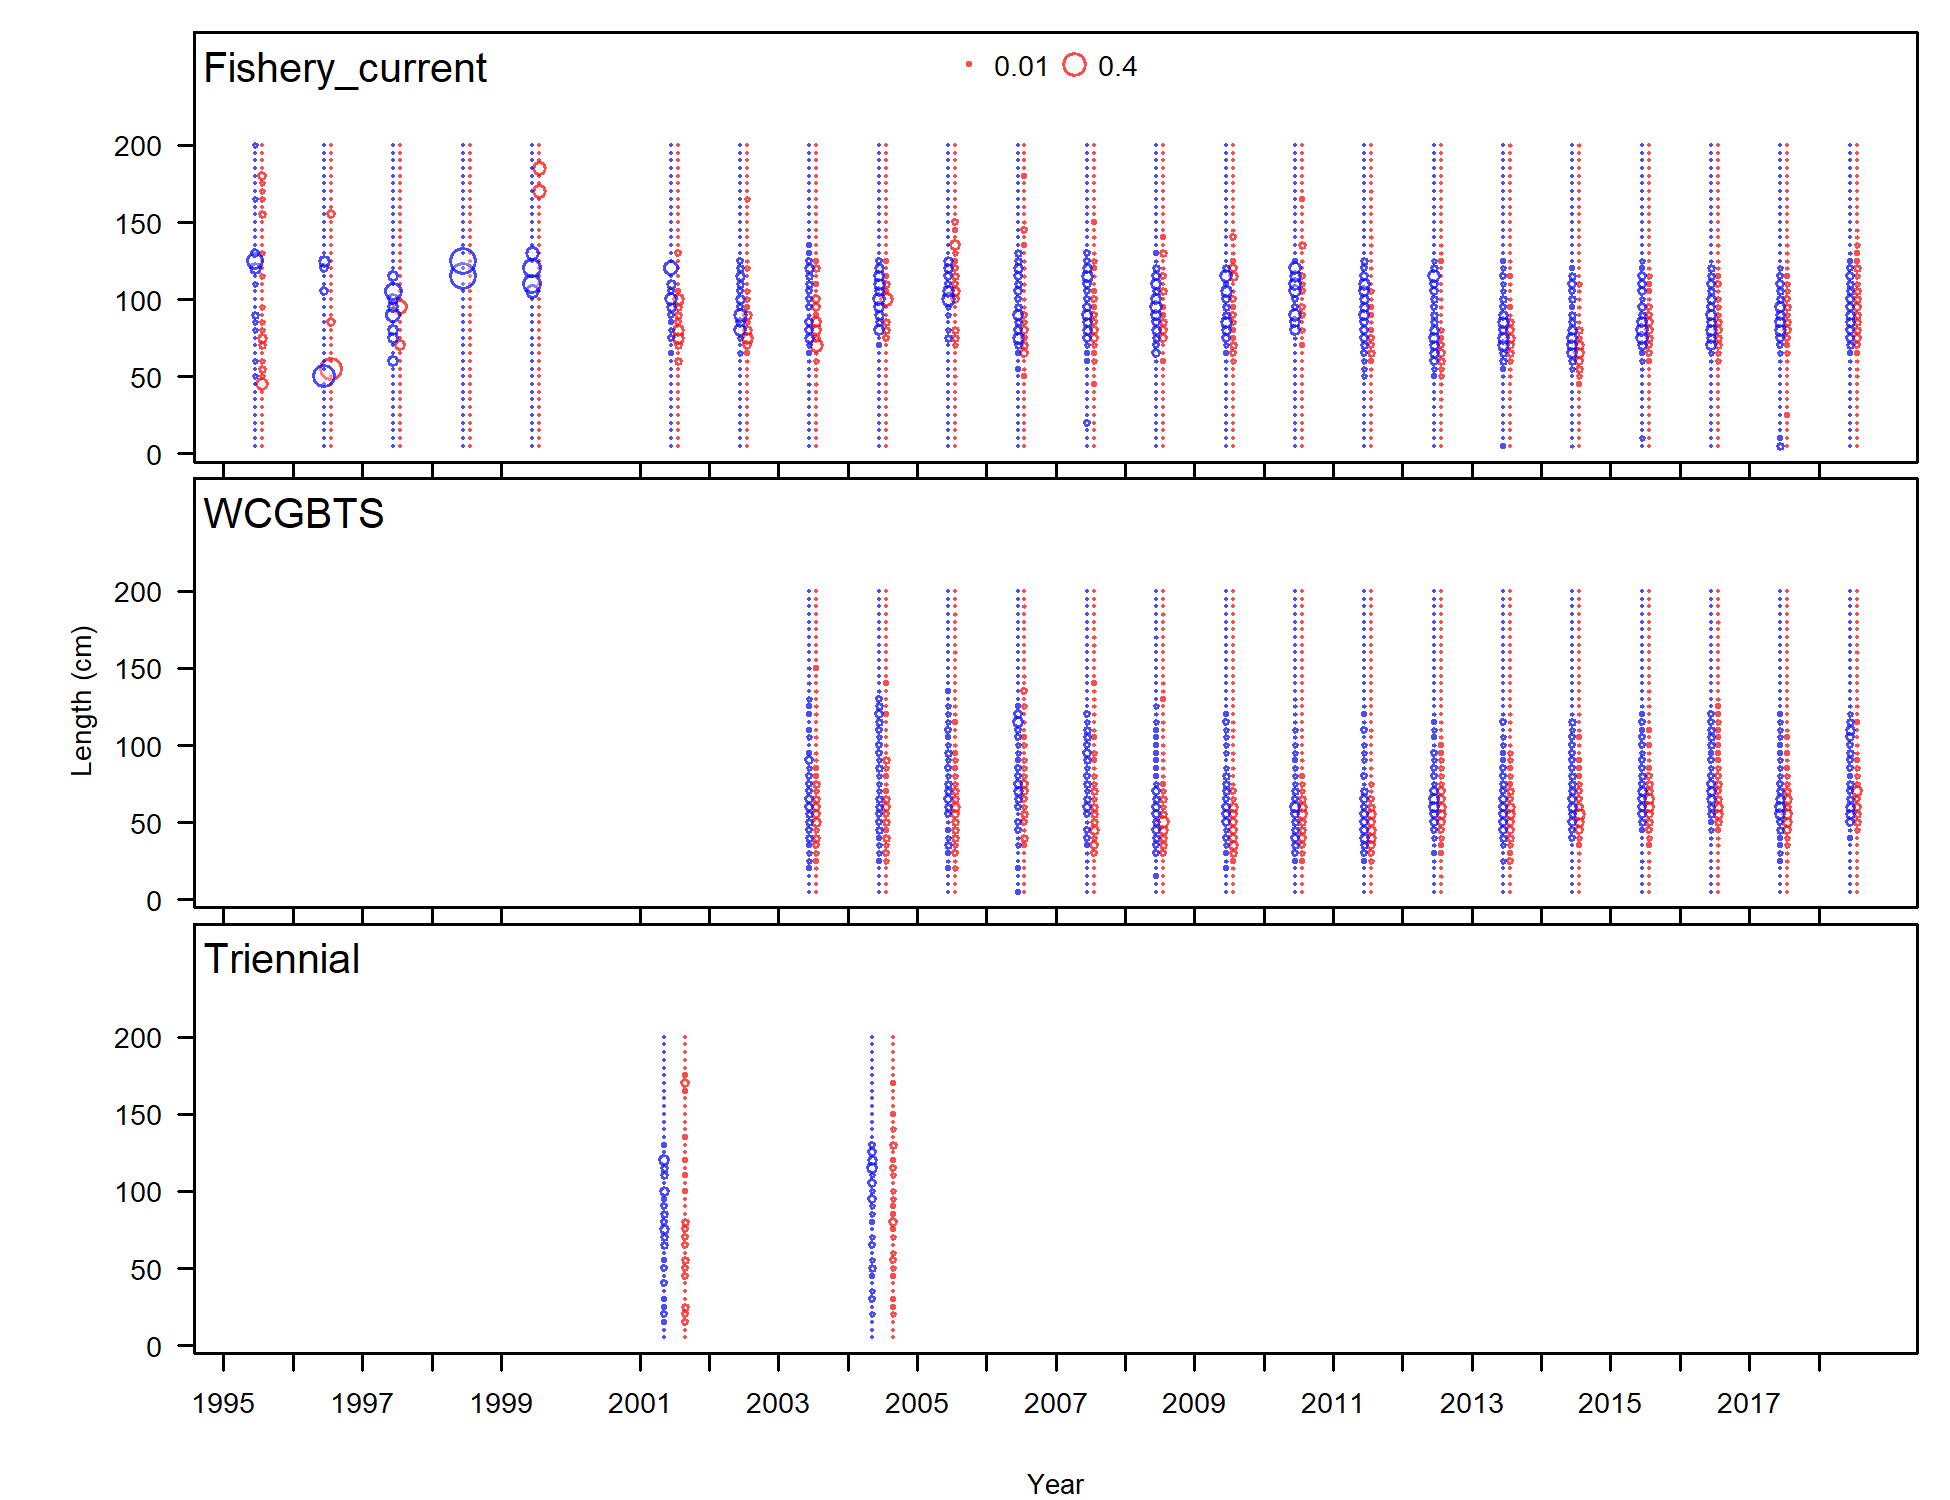
\includegraphics{r4ss/plots_mod1/comp_lendat__multi-fleet_comparison.png}
\caption{Length comp data for all years and fleets. Bubble size
indicates the observed proportions, with females in red and males in
blue. \label{fig:comp_lendat__multi-fleet_comparison}}
\end{figure}

\begin{figure}
\centering
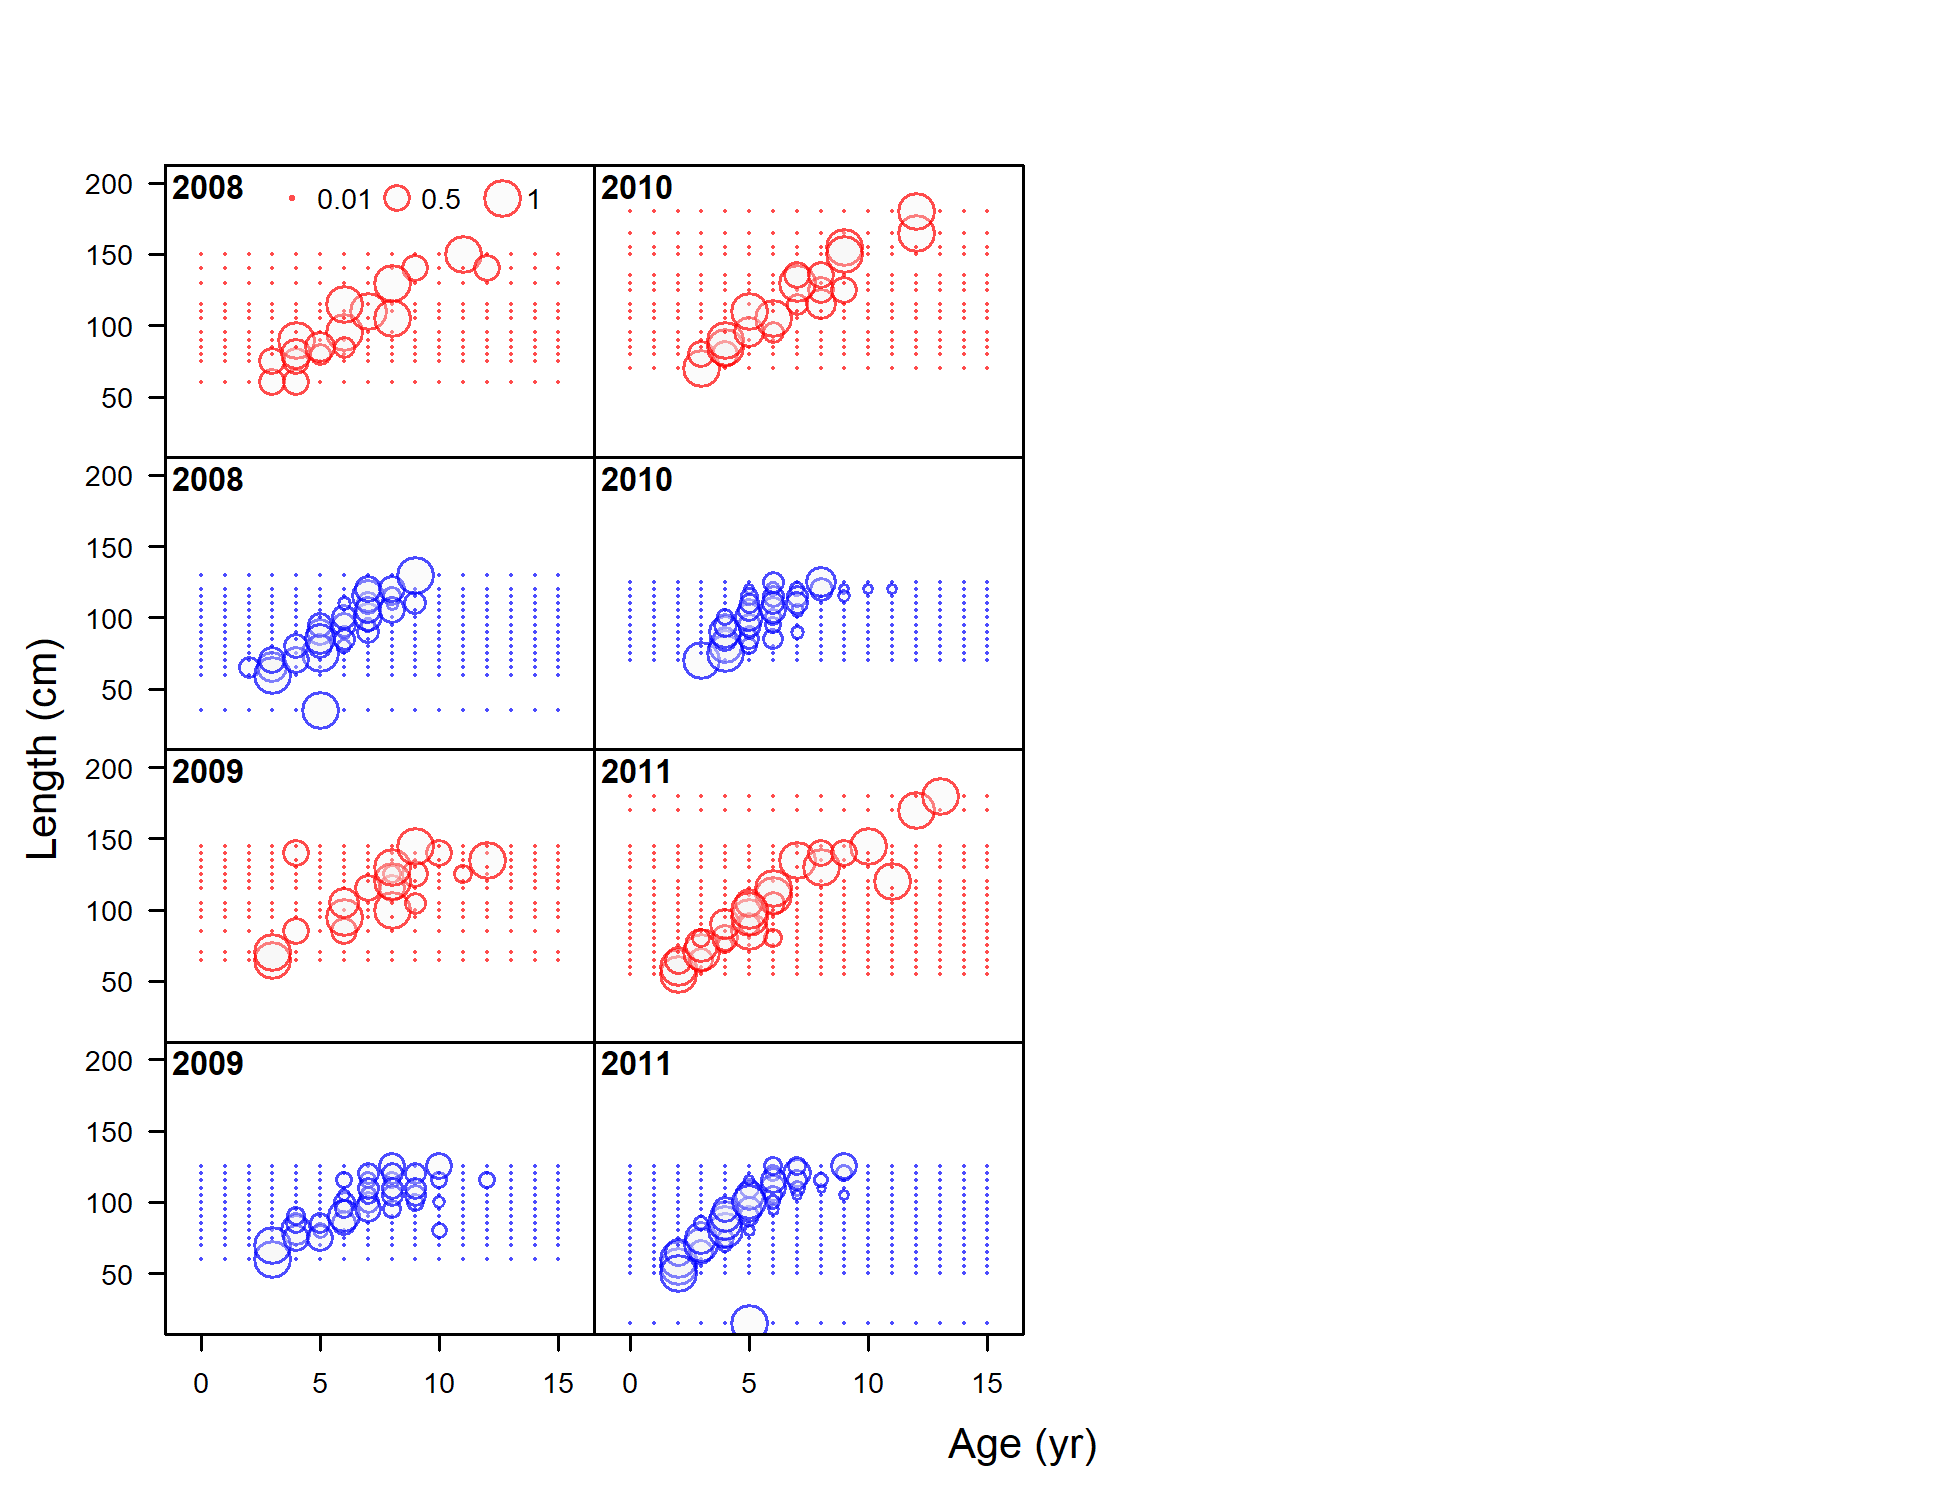
\includegraphics{r4ss/plots_mod1/comp_condAALdat_bubflt1mkt2.png}
\caption{Conditional age-at-length data from the fishery.
\label{fig:age_dat_fishery}}
\end{figure}

\begin{figure}
\centering
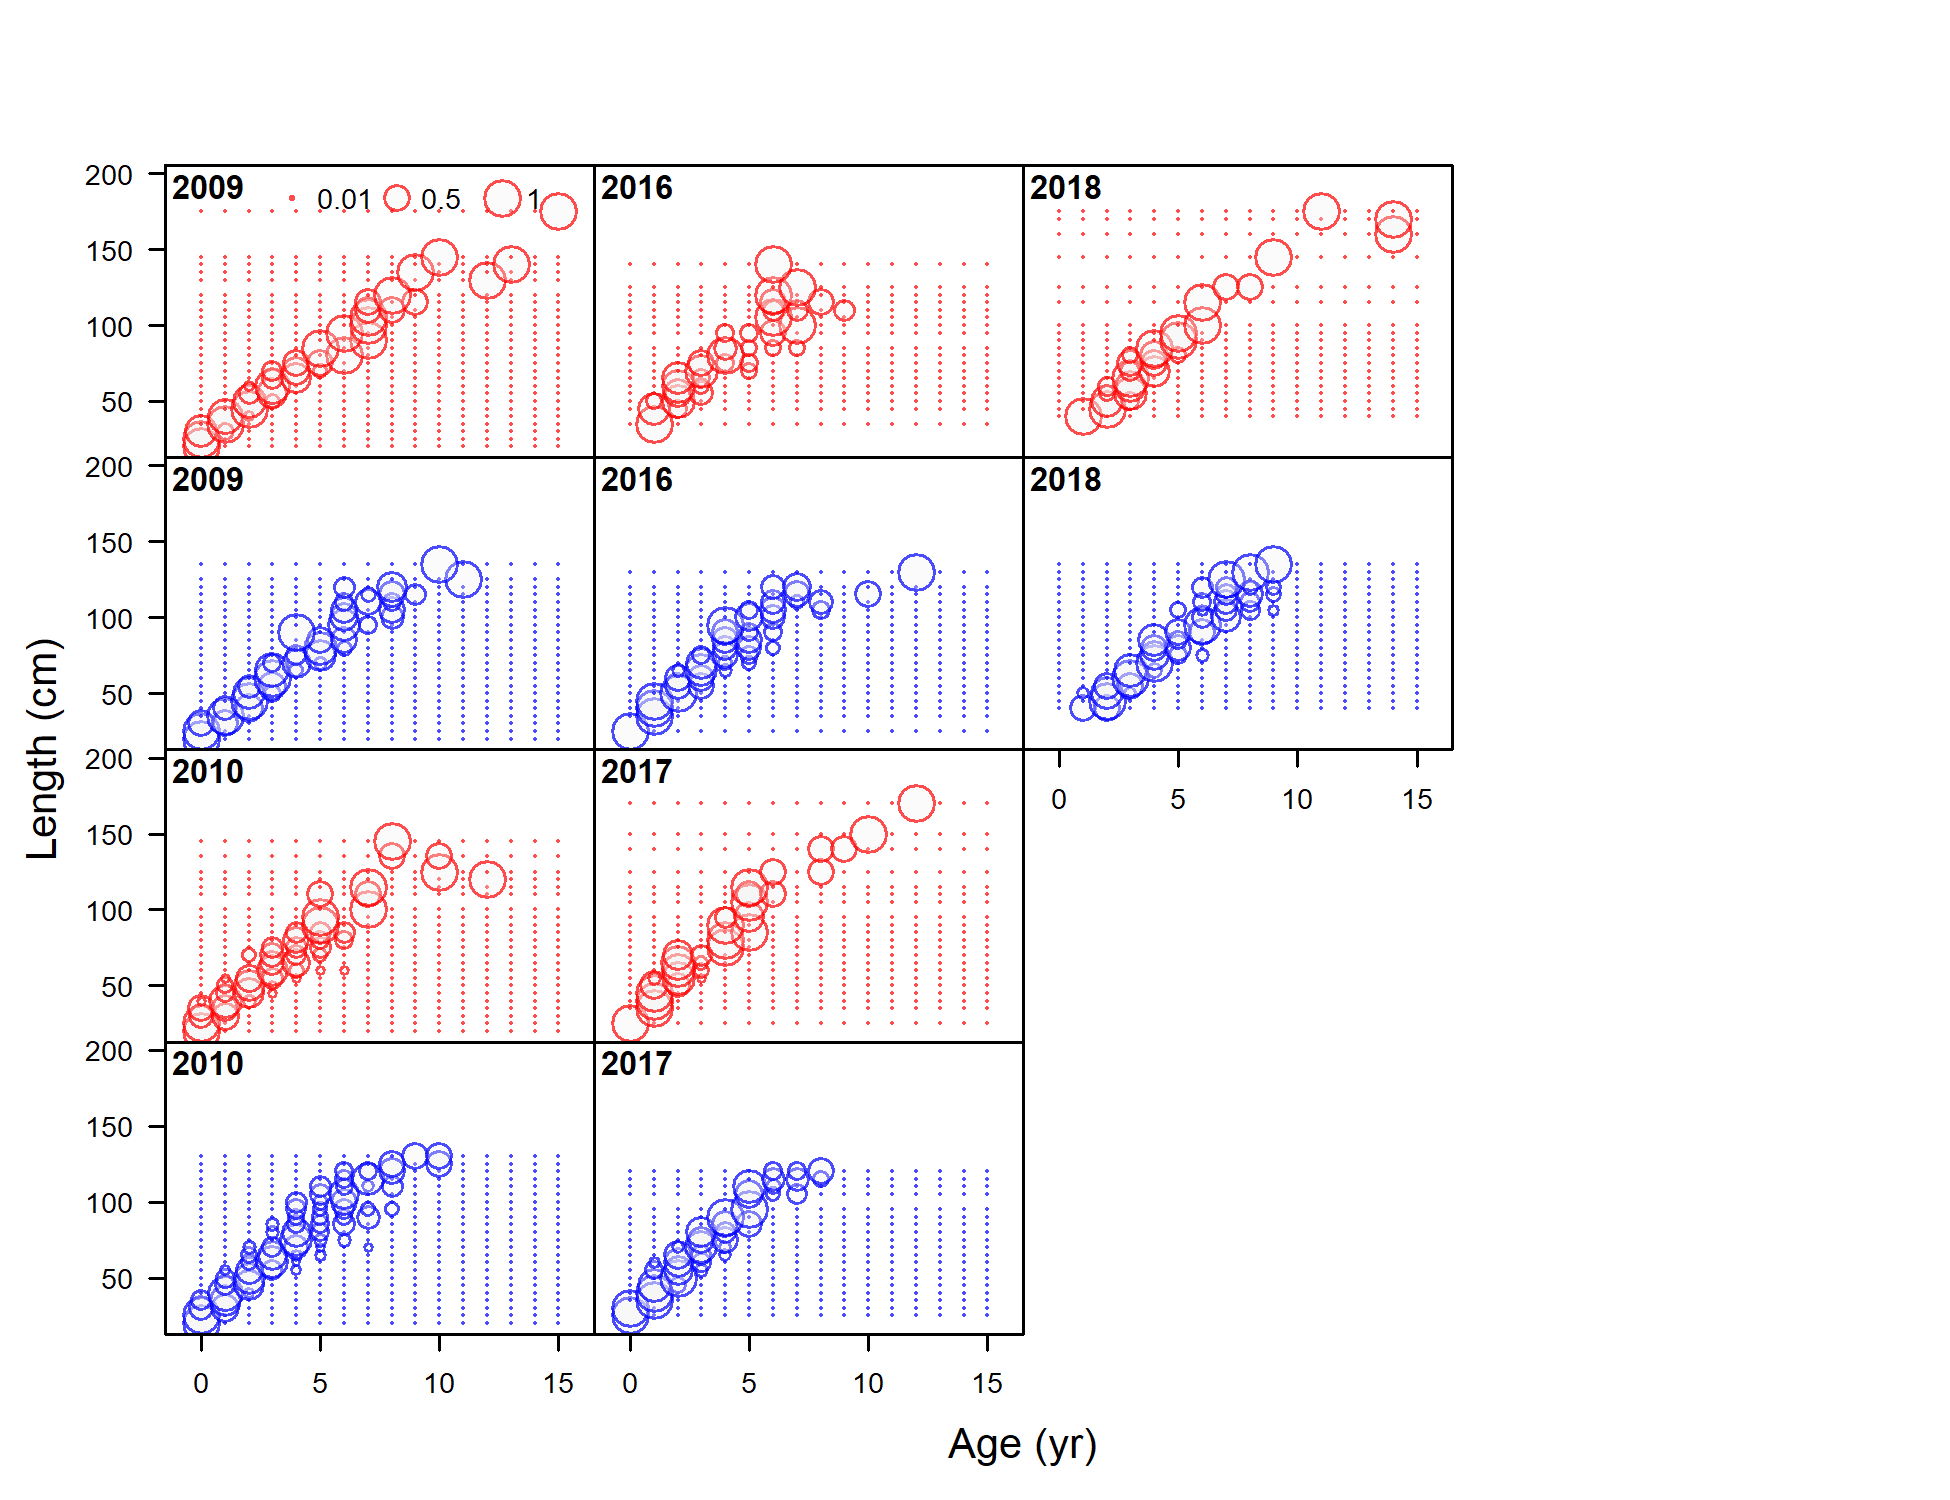
\includegraphics{r4ss/plots_mod1/comp_condAALdat_bubflt5mkt0.png}
\caption{Conditional age-at-length data from the WCGBT Survey.
\label{fig:age_dat_fishery}}
\end{figure}

\begin{figure}
\centering
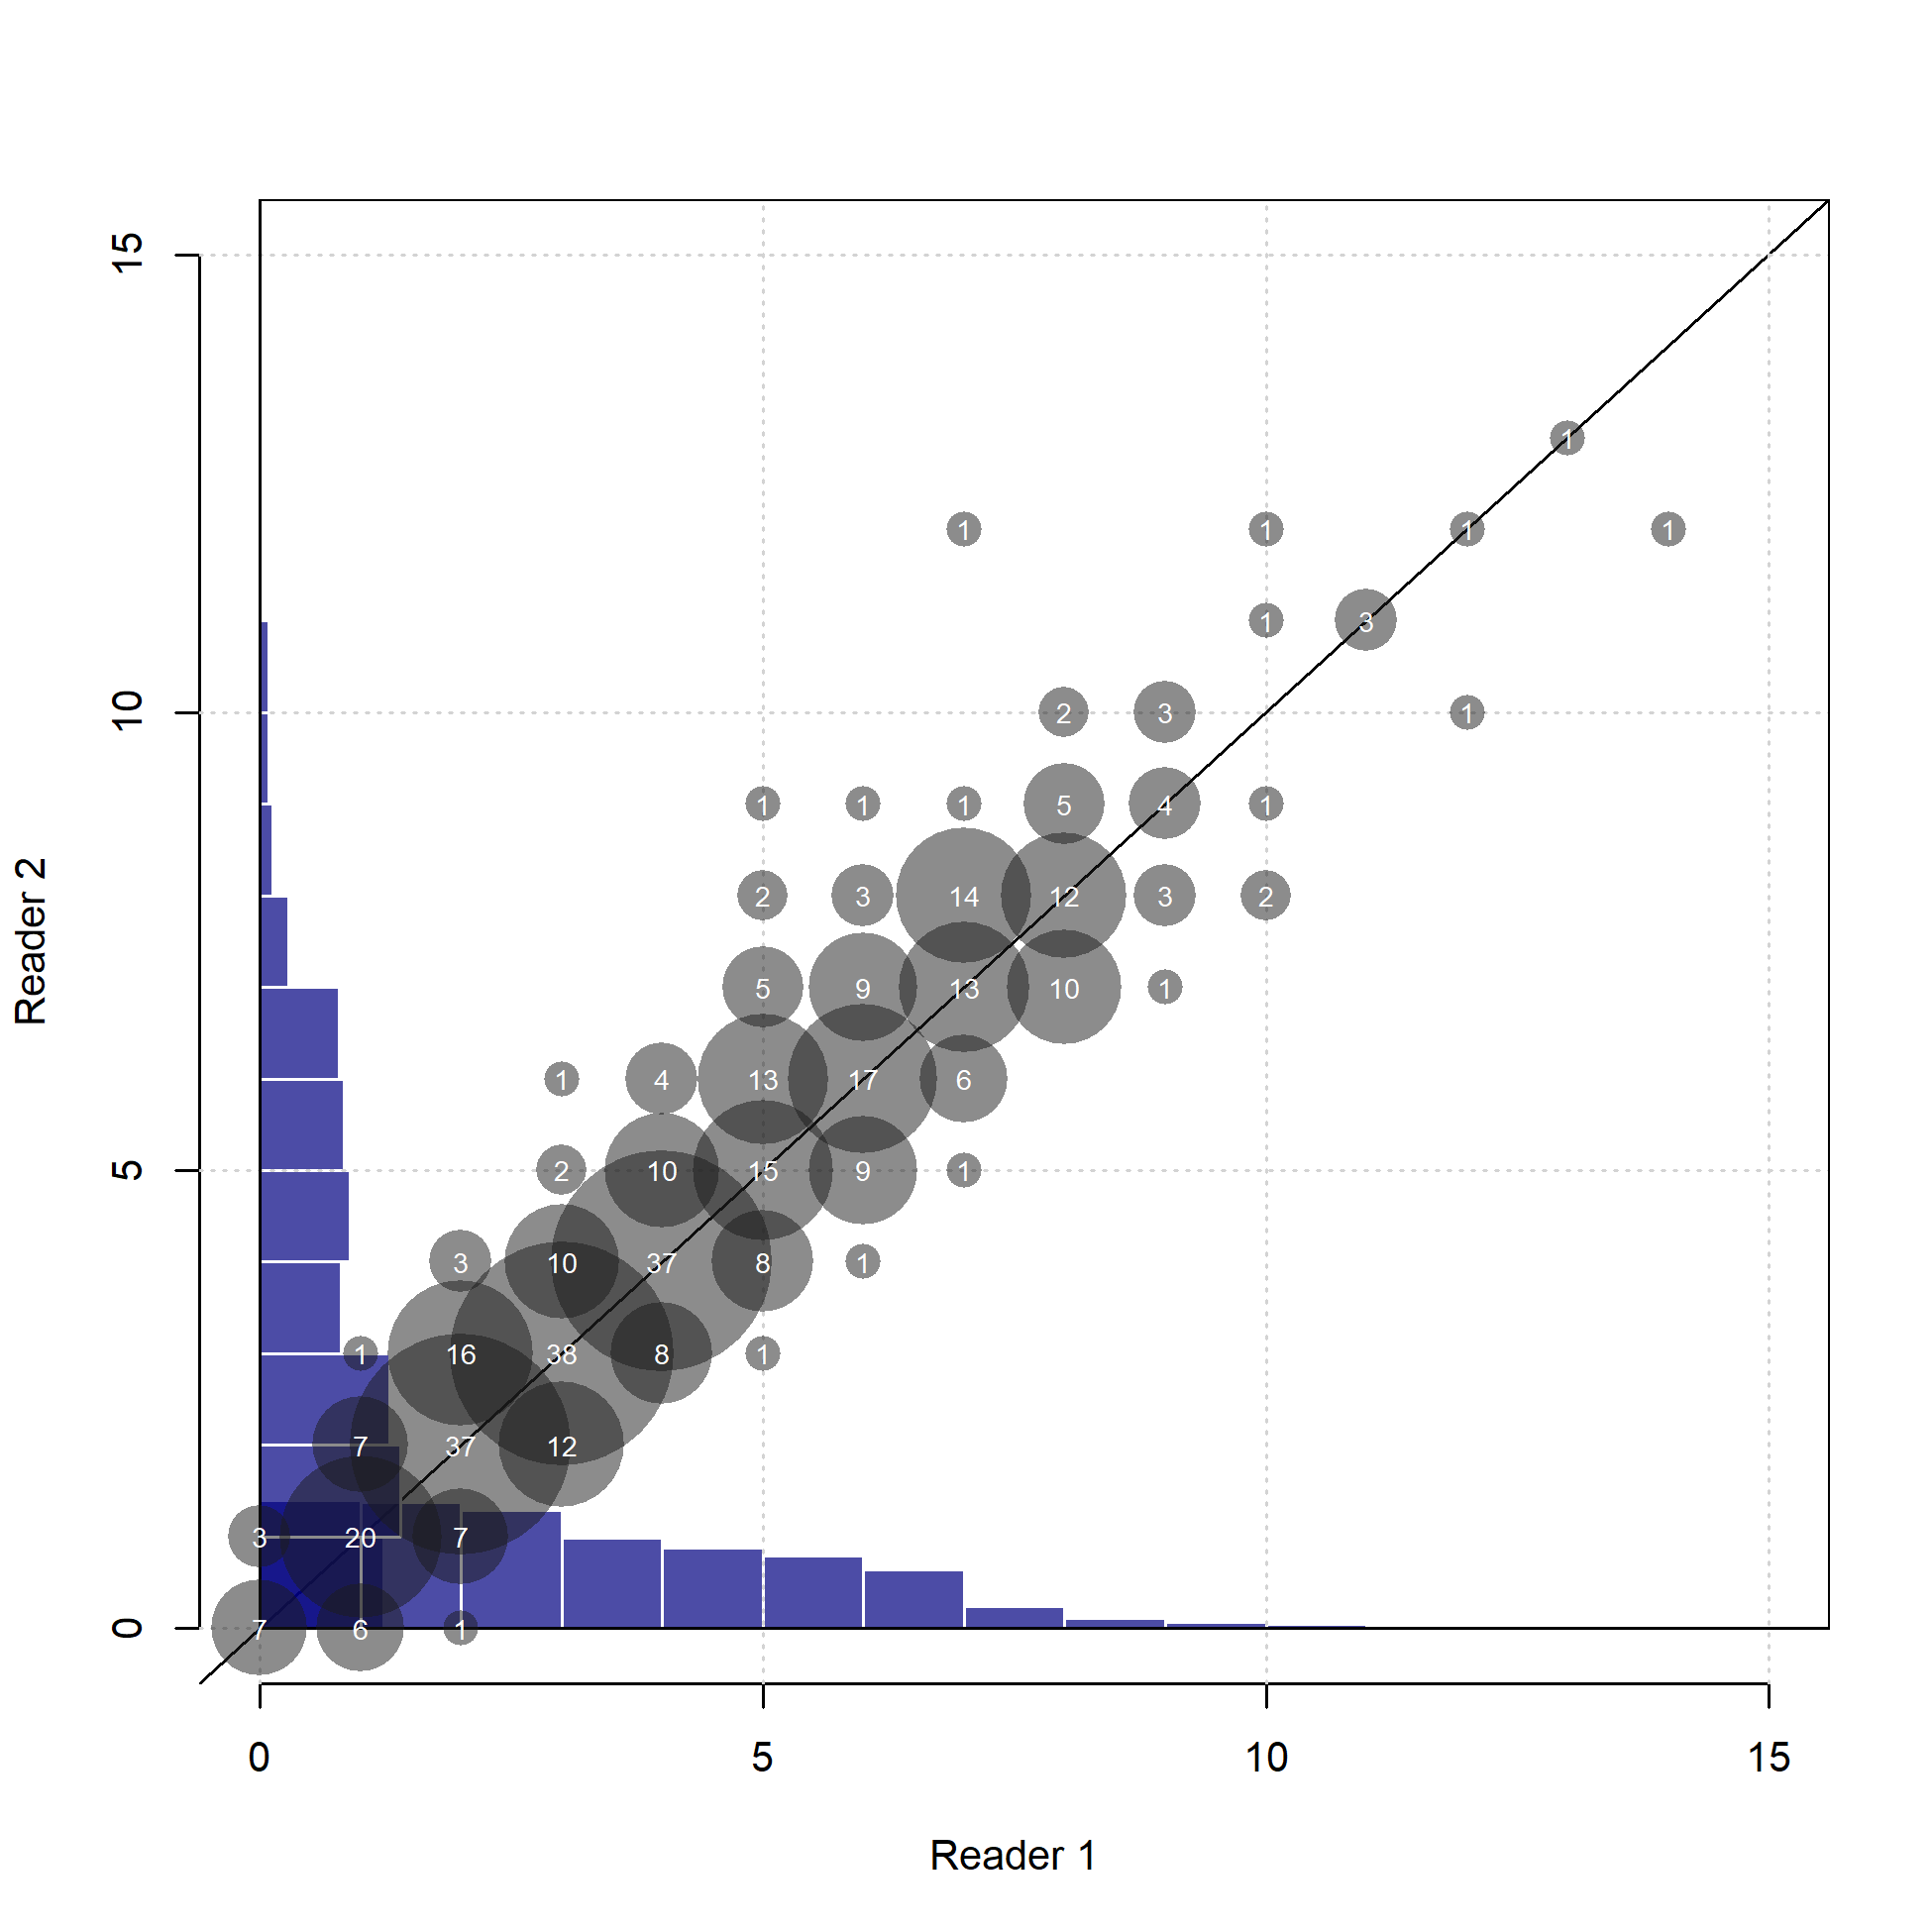
\includegraphics{Figures/Reader_1_vs_Reader_2.png}
\caption{Comparison of reads from each of two age readers for Big Skate.
Sample sizes associated with each combination of ages are shown by the
size circles and the within them. The blue histograms show the
distribution of ages estimated by each
reader.\label{fig:ageing_comparison}}
\end{figure}

\begin{figure}
\centering
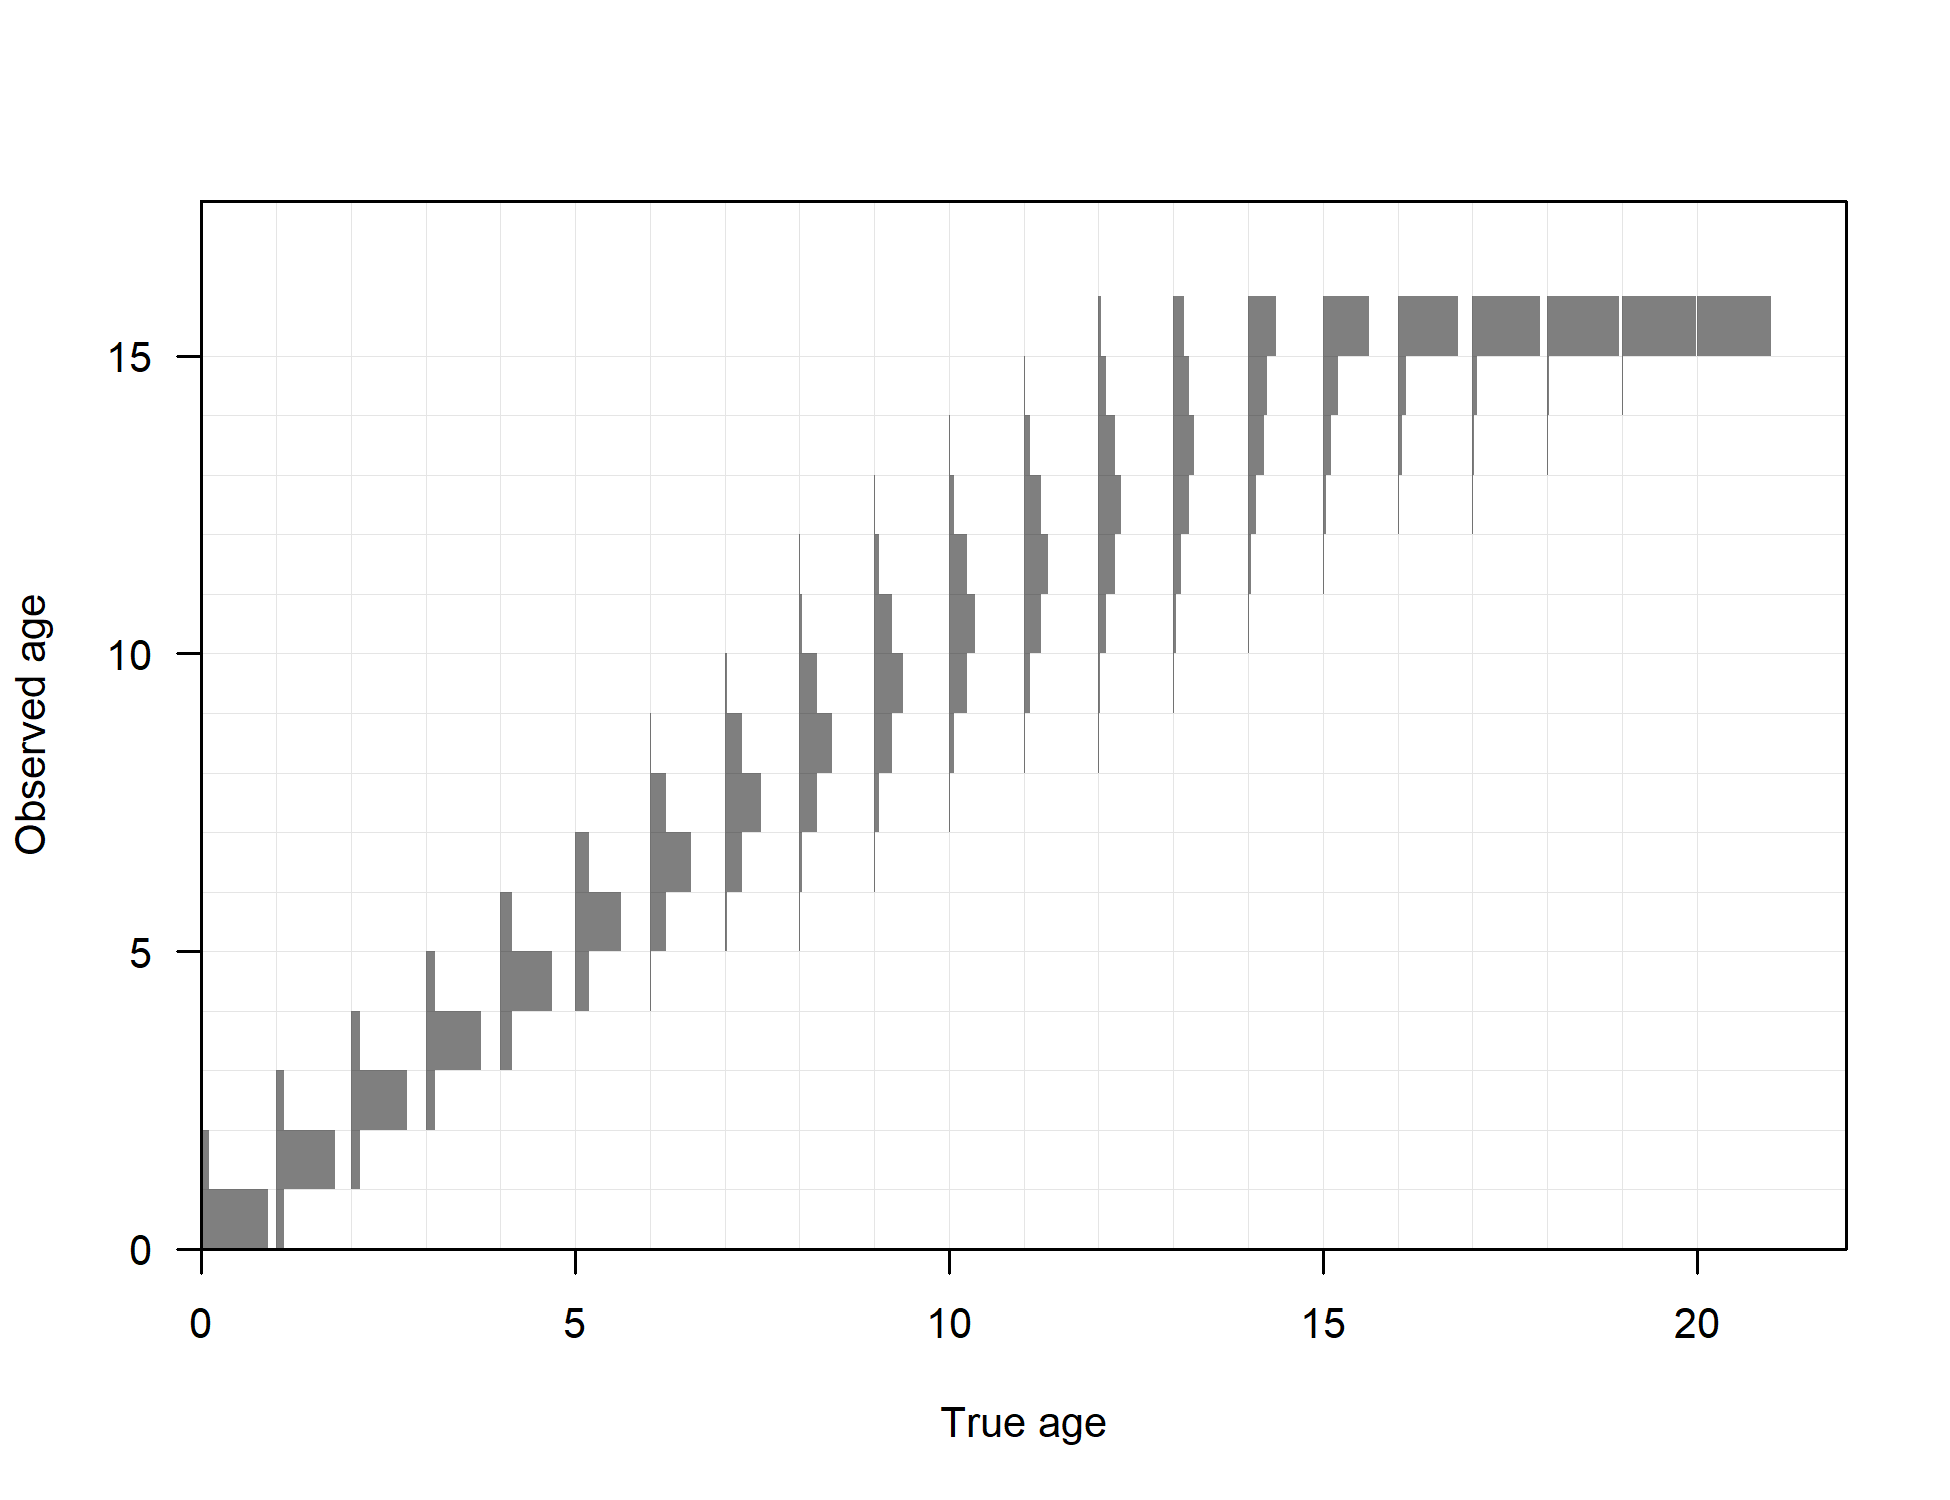
\includegraphics{r4ss/plots_mod1/numbers10_ageerror_matrix_1.png}
\caption{Estimated ageing imprecision.\label{fig:ageing_imprecision}}
\end{figure}

\begin{figure}
\centering
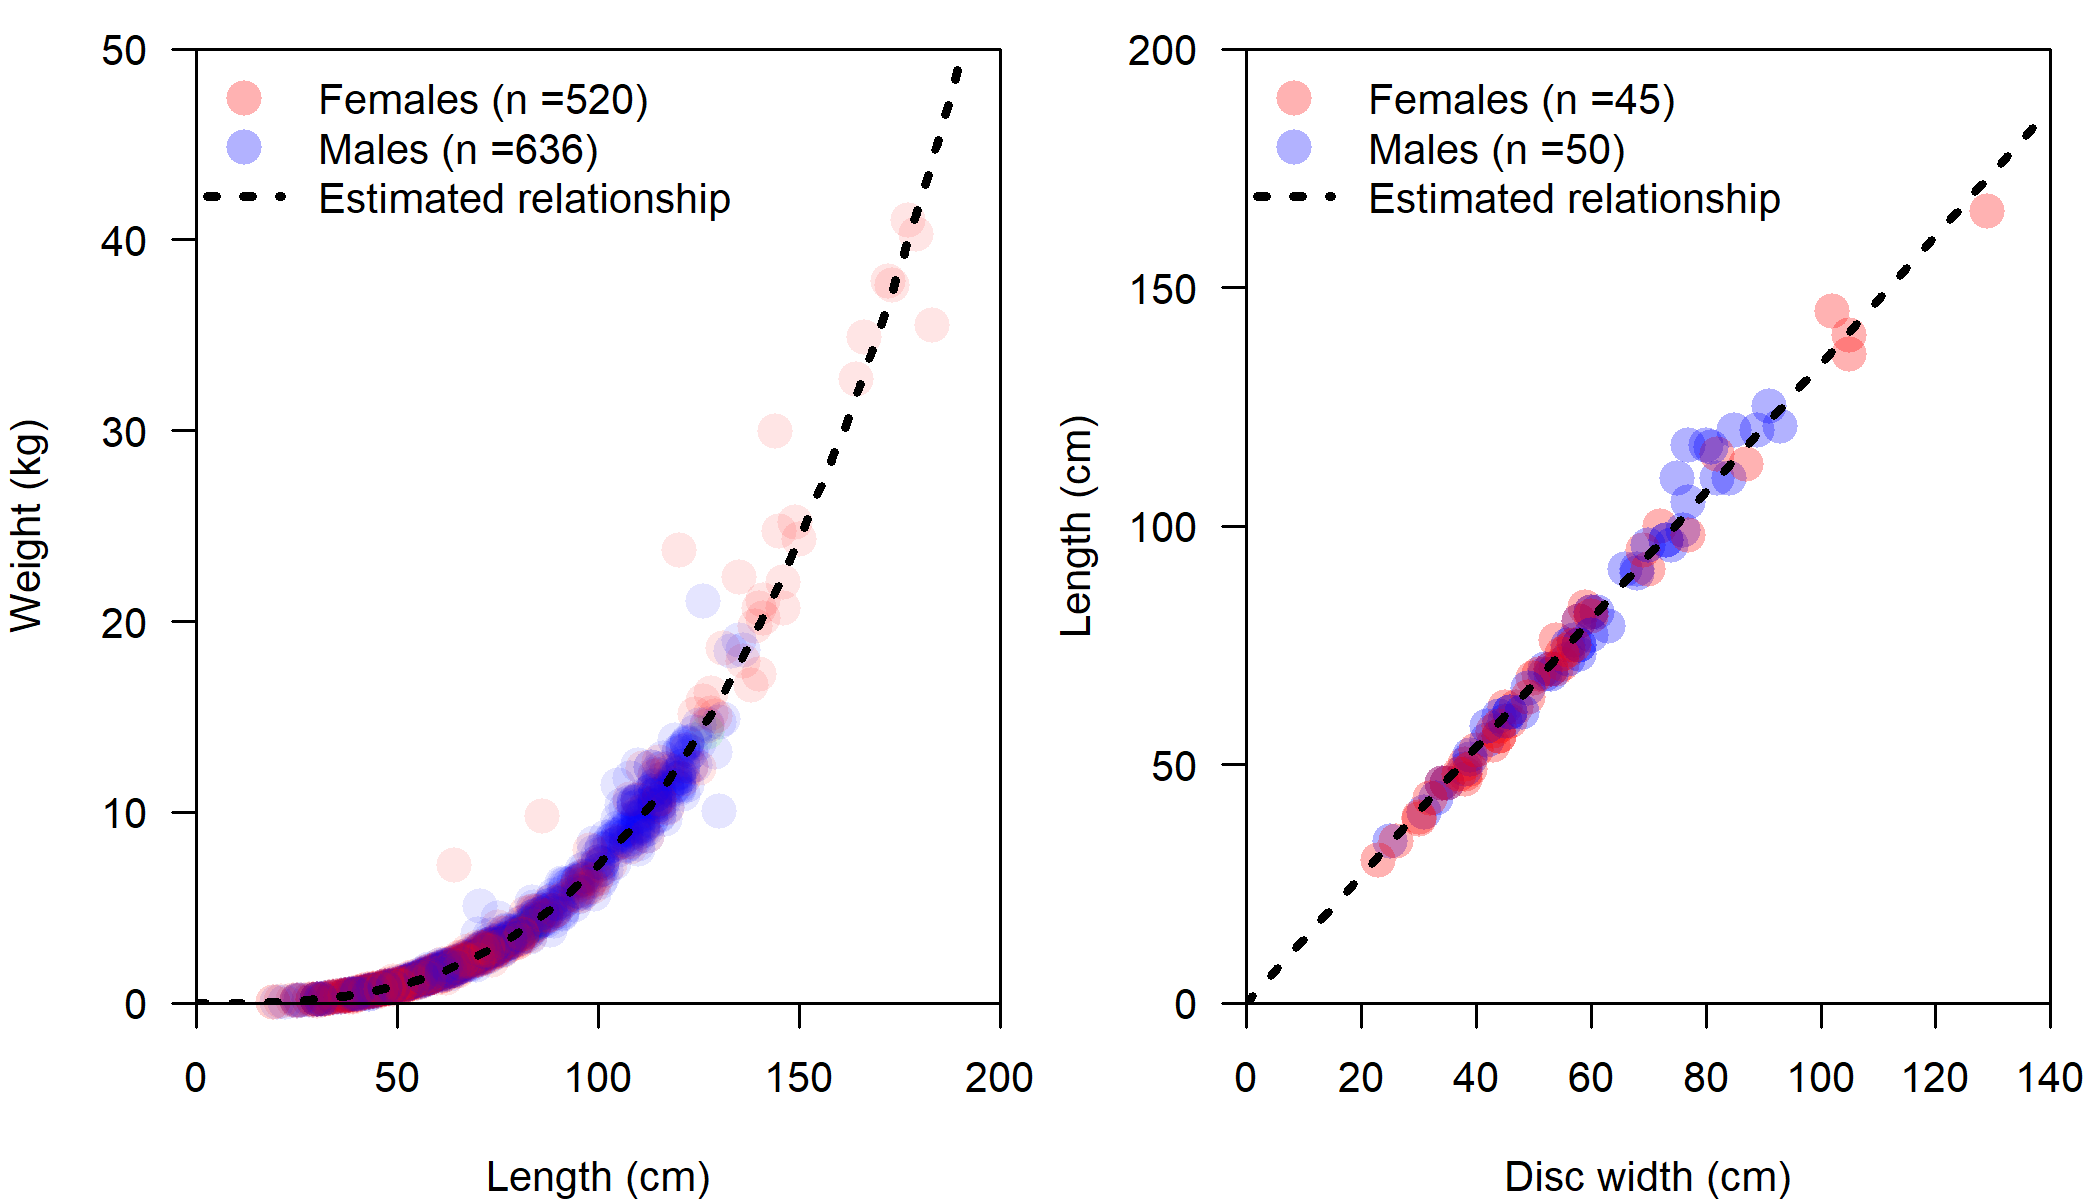
\includegraphics{Figures/Big Skate bio relationships.png}
\caption{Estimated relationship between length and weight (left) and
disc-width and length (right) for Big Skate. Colored points show
observed values and the black line indicates the estimated relationship
\(W = 0.0000074924L^{2.9925}\).\label{fig:weight-length}}
\end{figure}

\begin{figure}
\centering
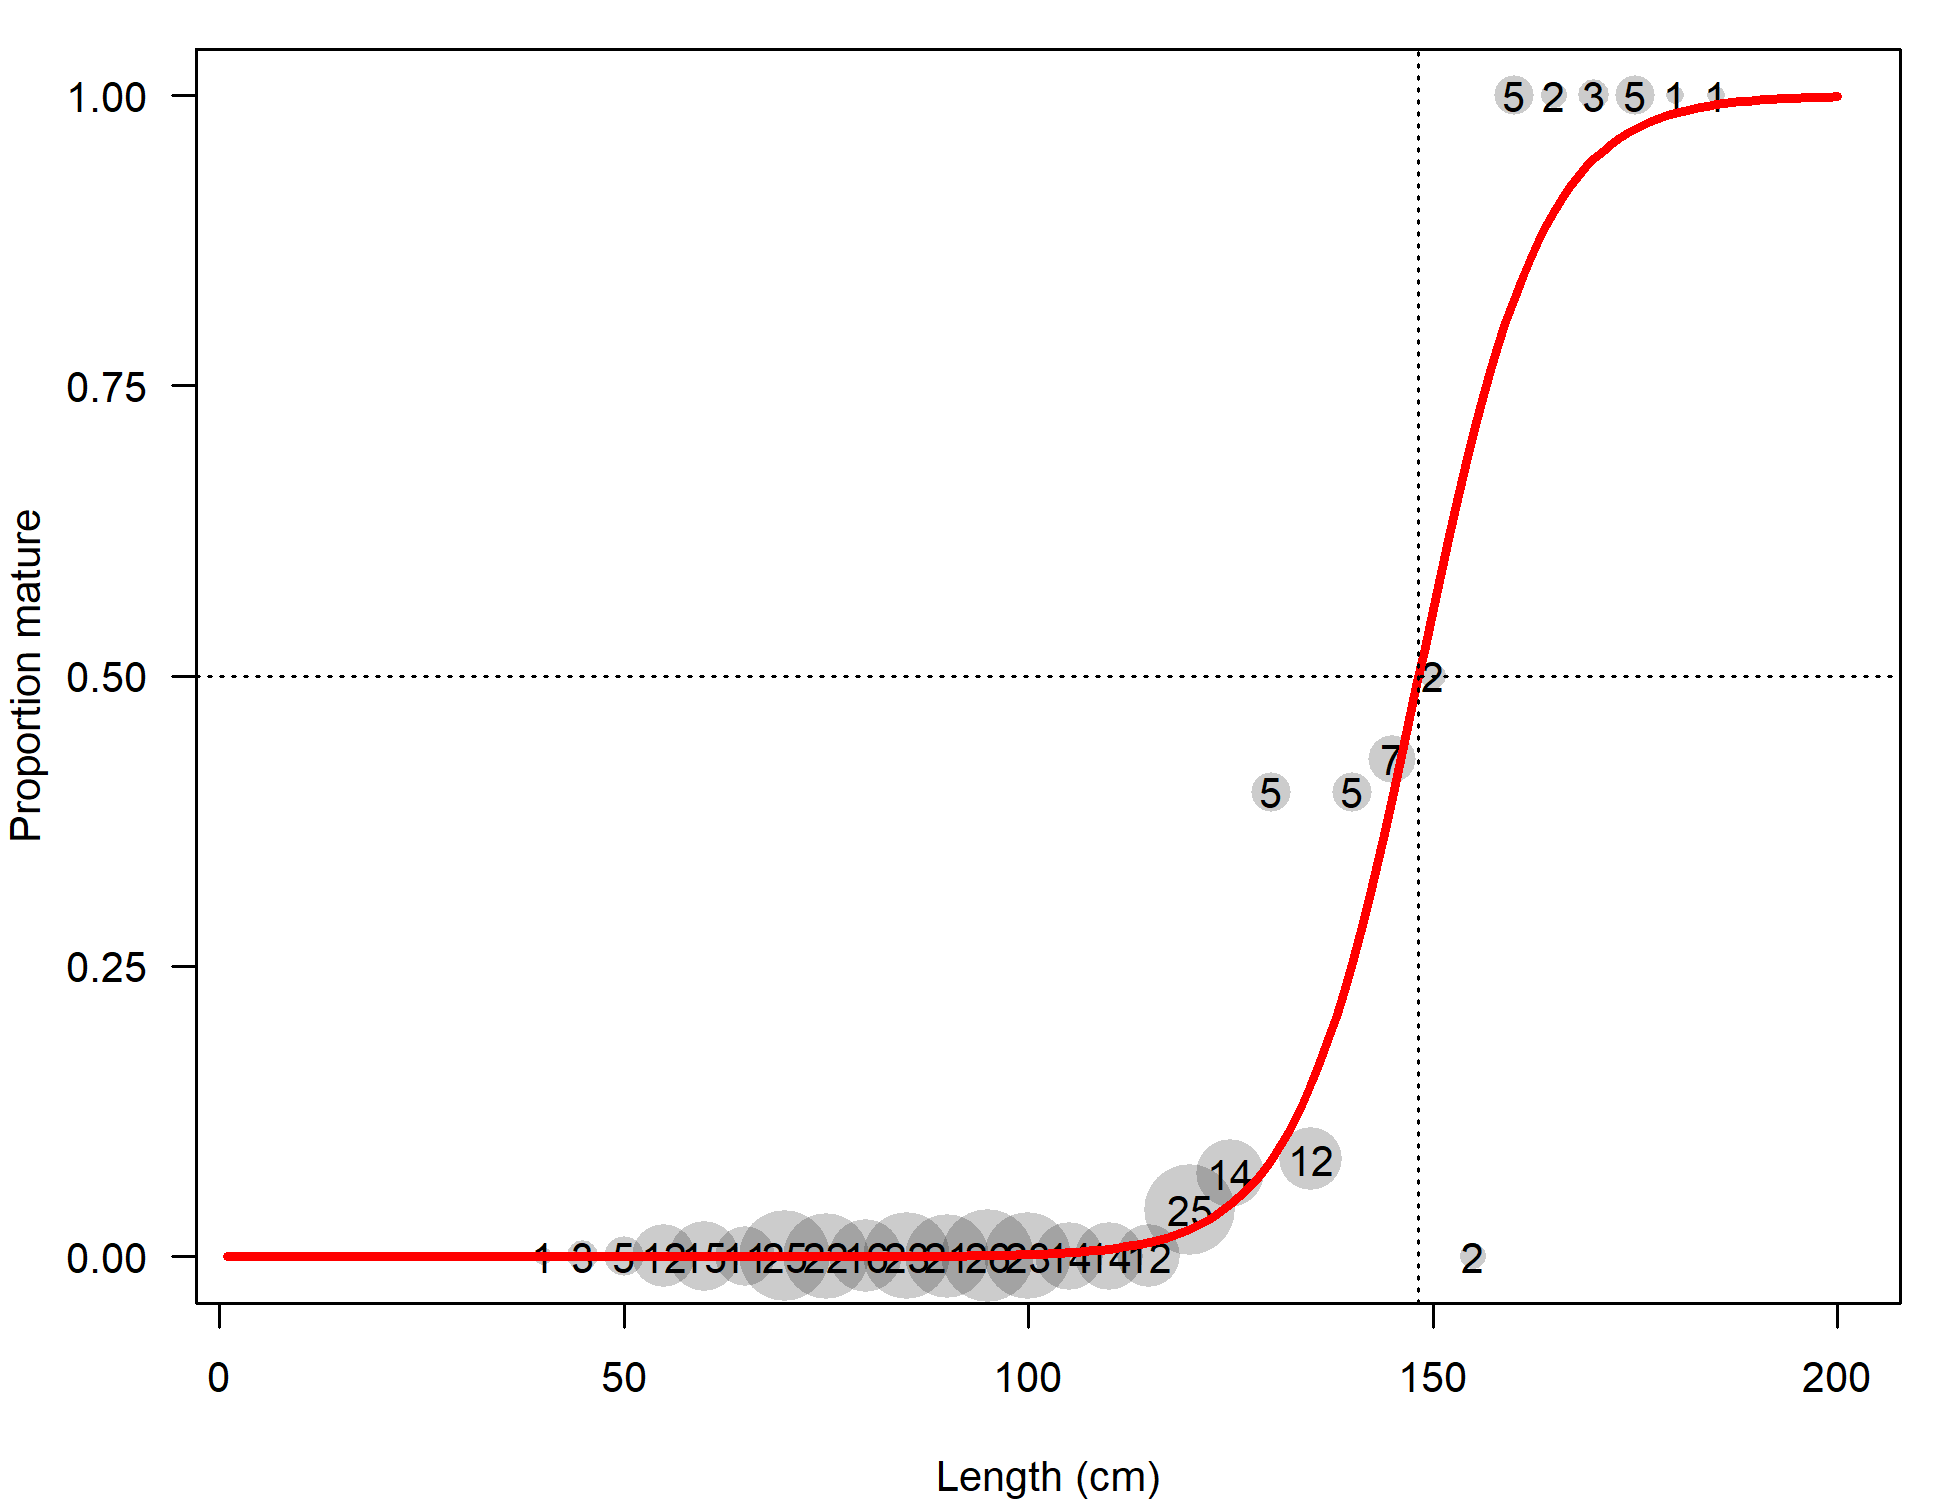
\includegraphics{Figures/BigSkate_maturity.png}
\caption{Estimated maturity relationship for female Big Skate. Gray
points indicate average observed functional maturity within each length
bin with point size proportional to the number of samples (indicated by
text within each point).\label{fig:maturity}}
\end{figure}

\FloatBarrier
\newpage

\FloatBarrier
\newpage

\hypertarget{model-results-figures}{%
\subsection{Model Results Figures}\label{model-results-figures}}

\FloatBarrier

\textbackslash{}begin\{figure\}{[}H{]}
\textbackslash{}begin\{centering\}
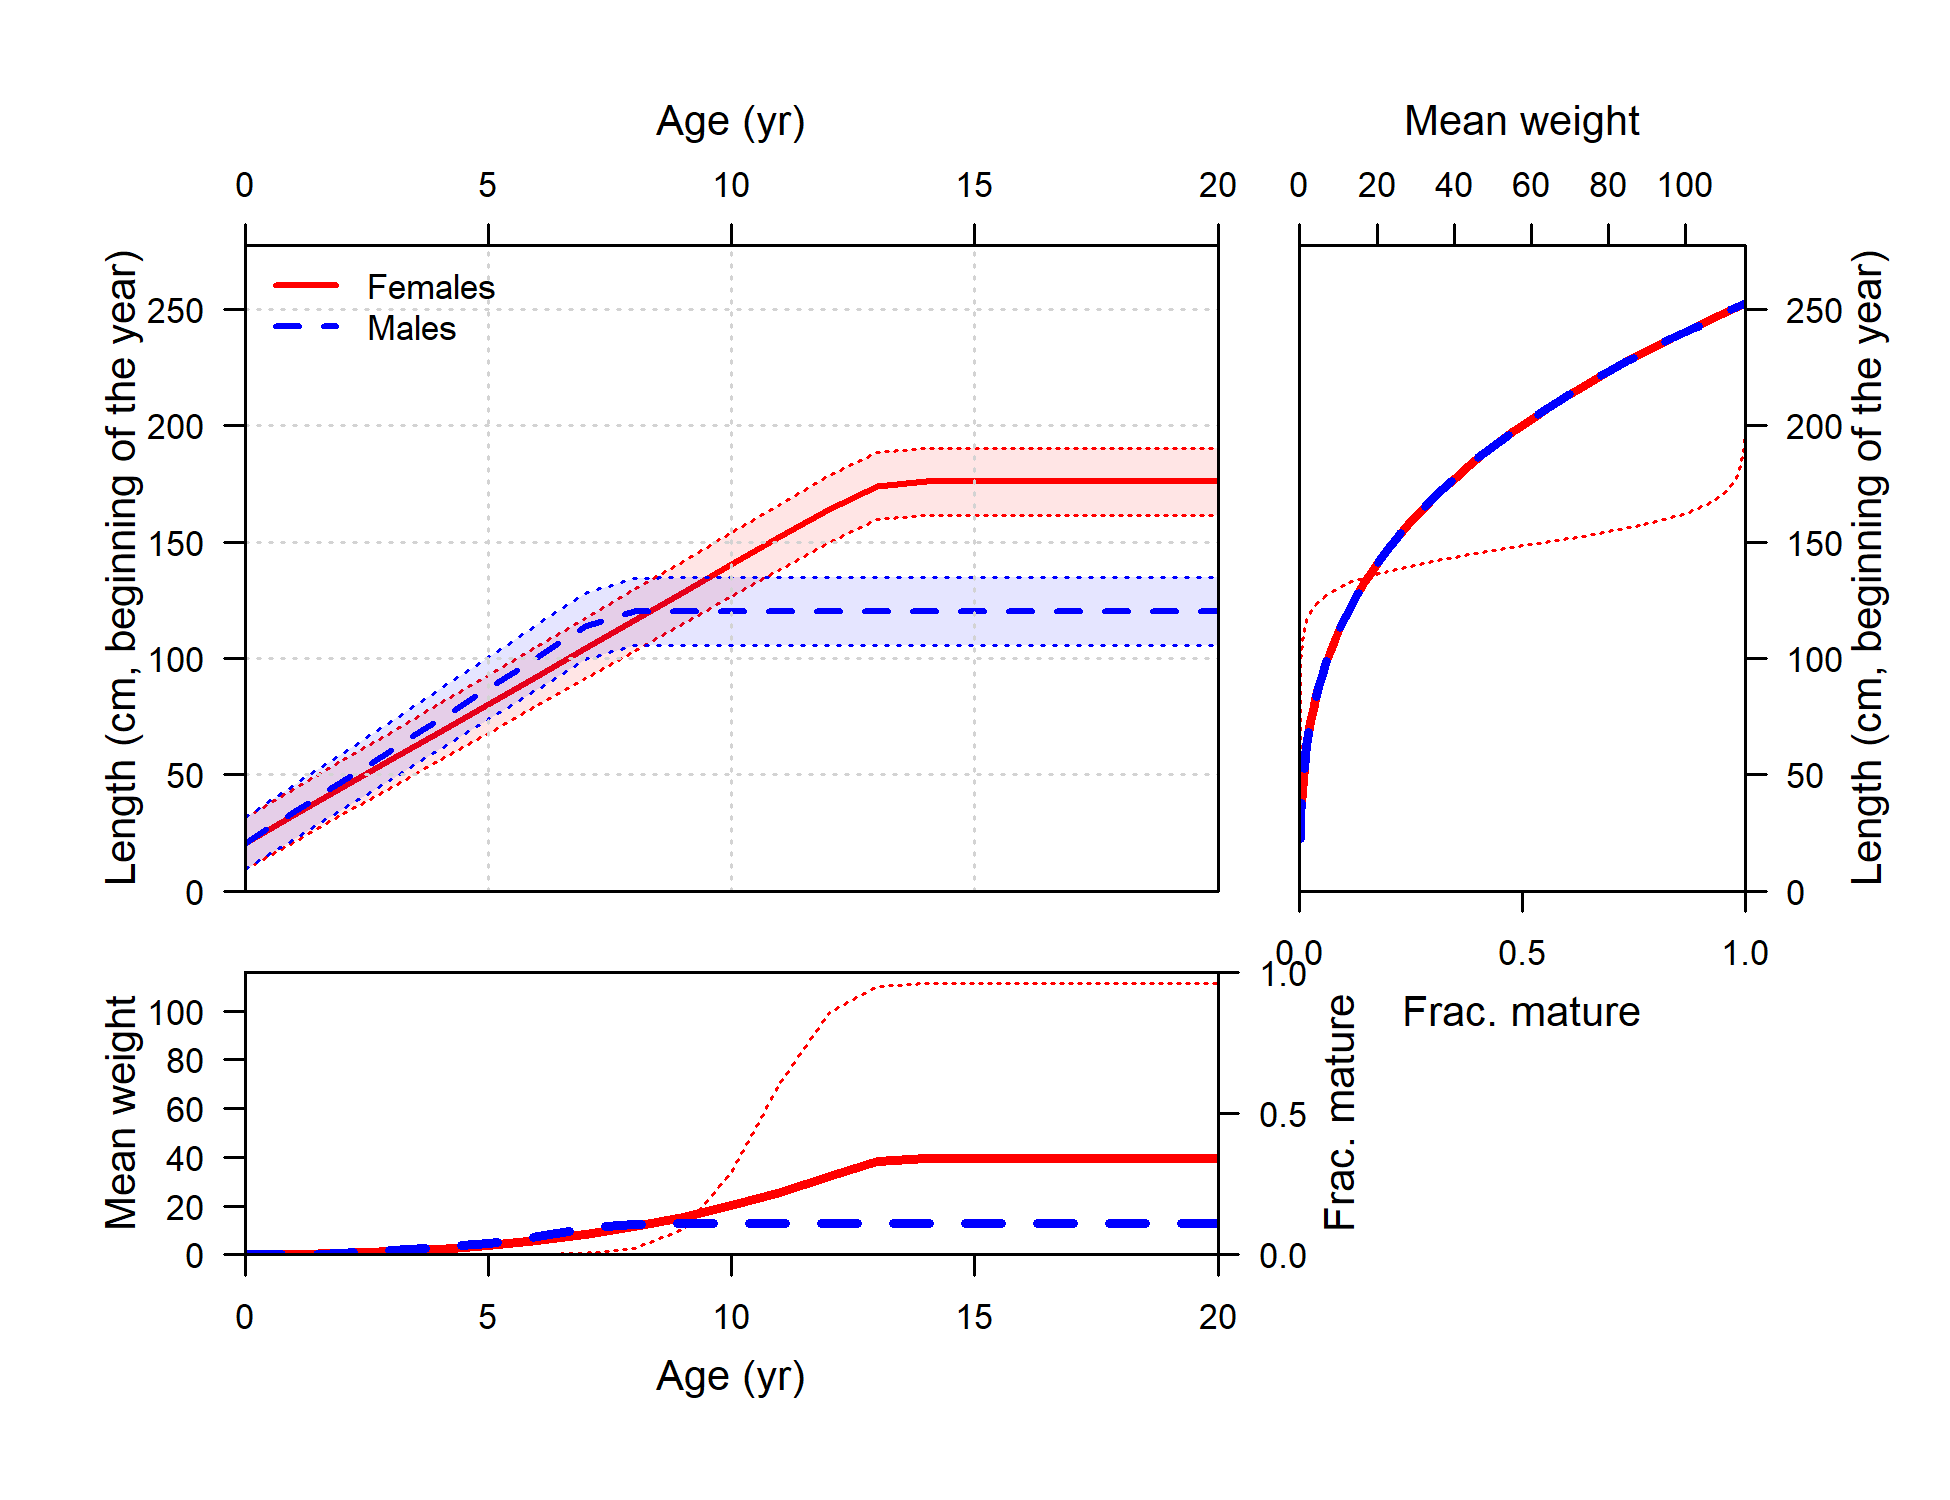
\includegraphics{r4ss/plots_mod1/bio3_sizeatage_plus_WT_and_MAT.png}
\textbackslash{}caption\{Estimated length-at-age for female and male Big
Skate (top left panel). Shaded areas indicate 95\% intervals for
distribution of lengths at each age. Values represent beginning-of-year
growth. Weight (thick line) and maturity (thin line) are shown in the
top-right and lower-left panels as a function of length and age,
respectively, where the values-at-age are calculated by mapping the
length-based relationships through the estimated distribution of length
at each age.\}\label{fig:growth} \textbackslash{}end\{centering\}
\textbackslash{}end\{figure\}

\FloatBarrier

\begin{figure}
\centering
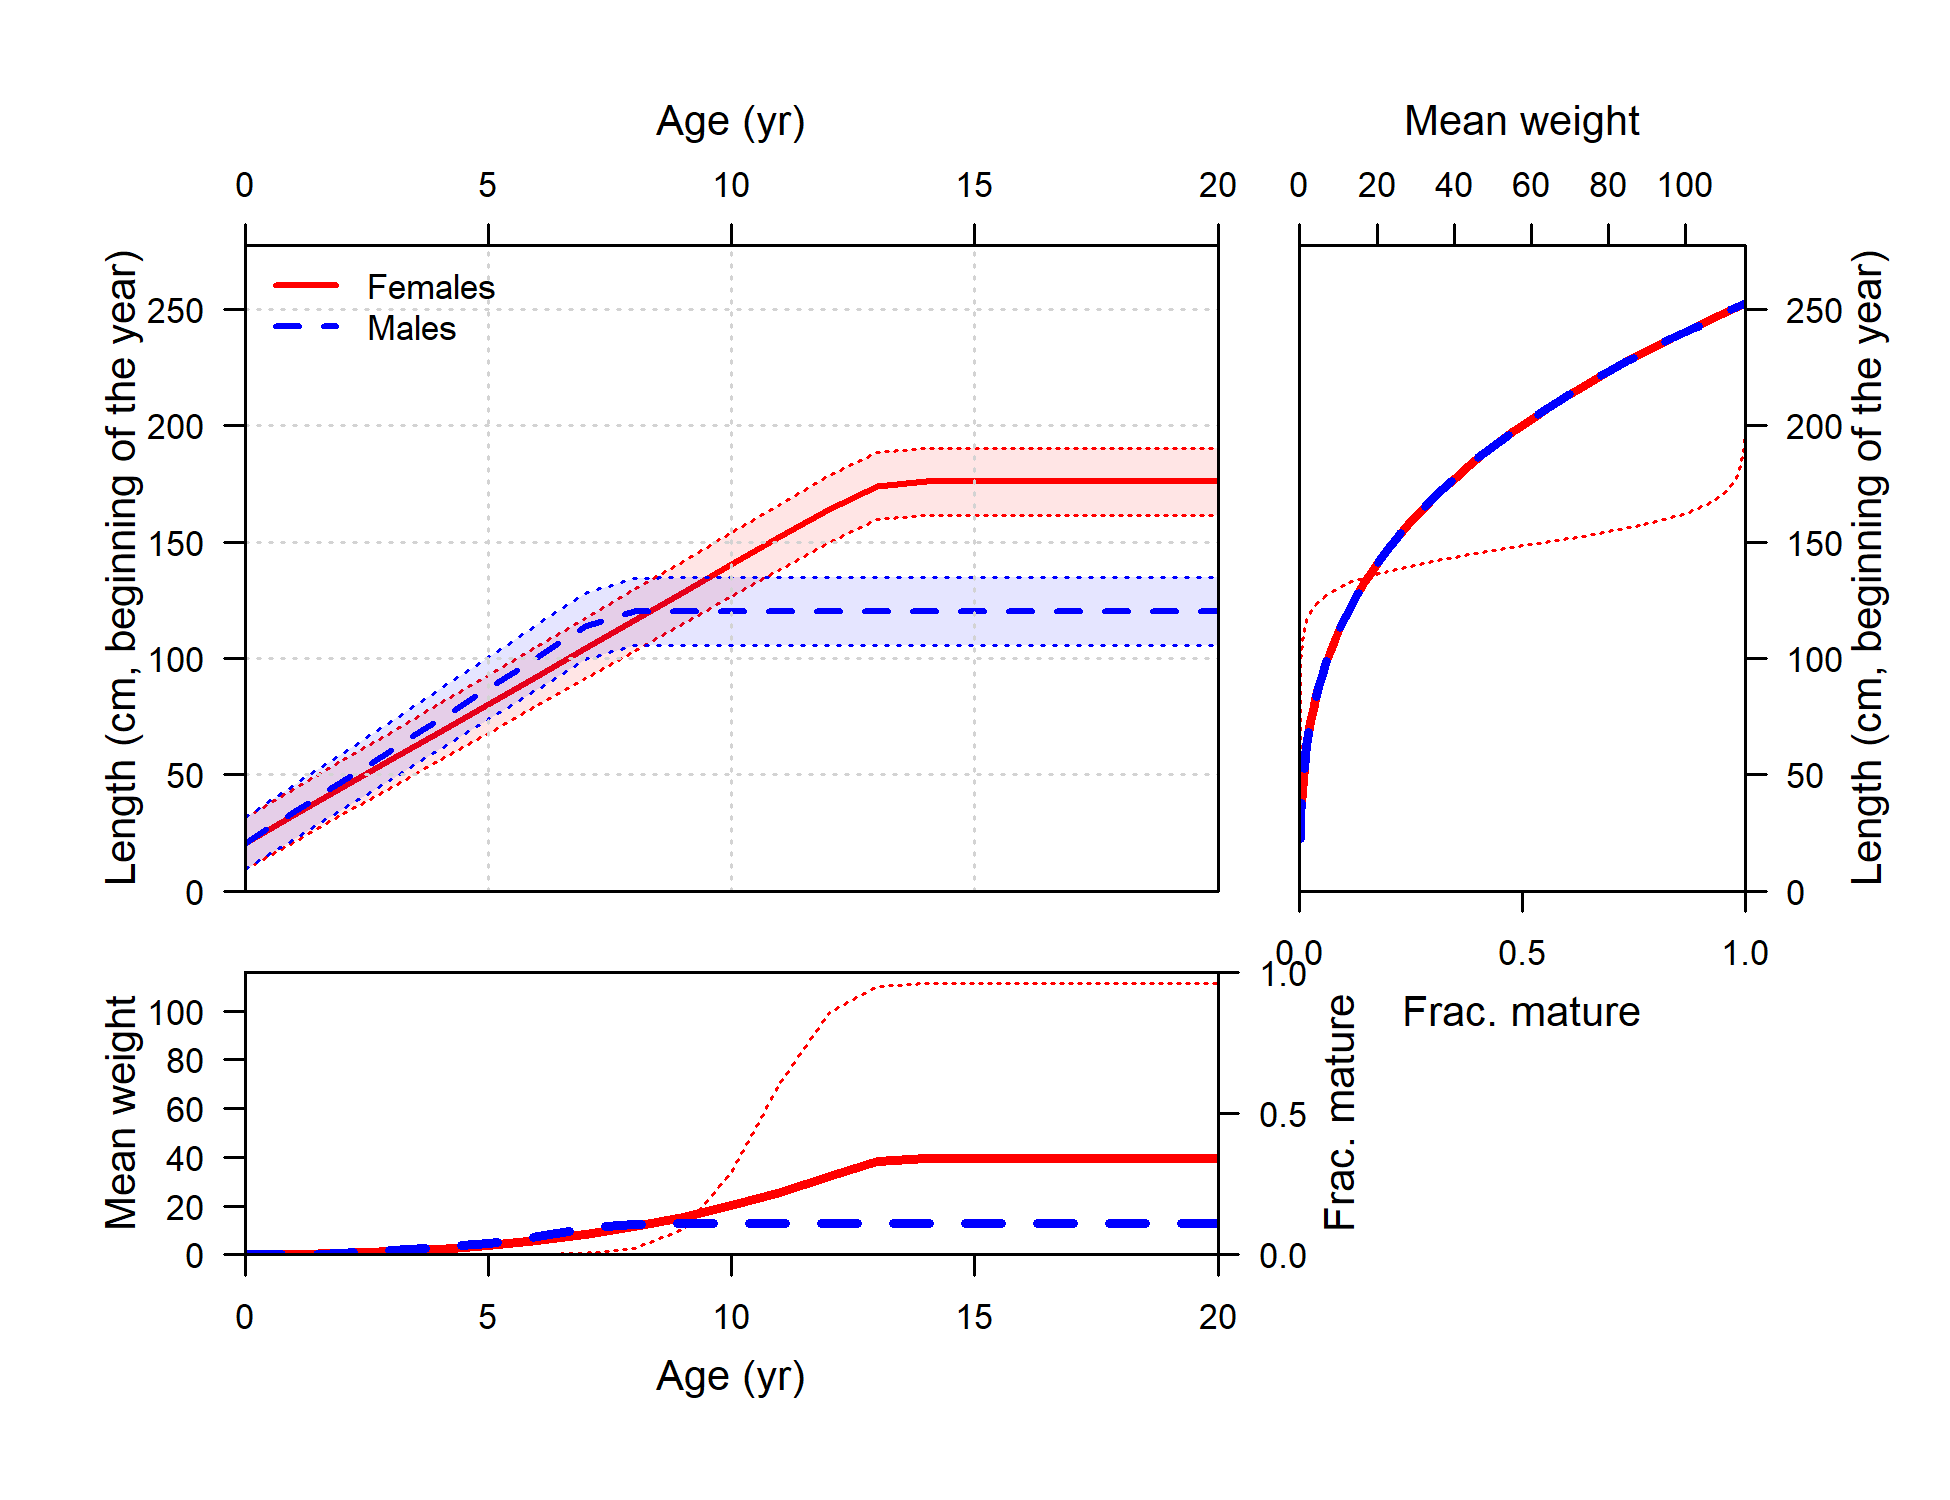
\includegraphics{r4ss/plots_mod1/bio3_sizeatage_plus_WT_and_MAT.png}
\caption{Estimated length-at-age for female and male Big Skate (top left
panel). Shaded areas indicate 95\% intervals for distribution of lengths
at each age. Values represent beginning-of-year growth. Weight (thick
line) and maturity (thin line) are shown in the top-right and lower-left
panels as a function of length and age, respectively, where the
values-at-age are calculated by mapping the length-based relationships
through the estimated distribution of length at each
age.\label{fig:growth}}
\end{figure}

\FloatBarrier

\begin{figure}
\centering
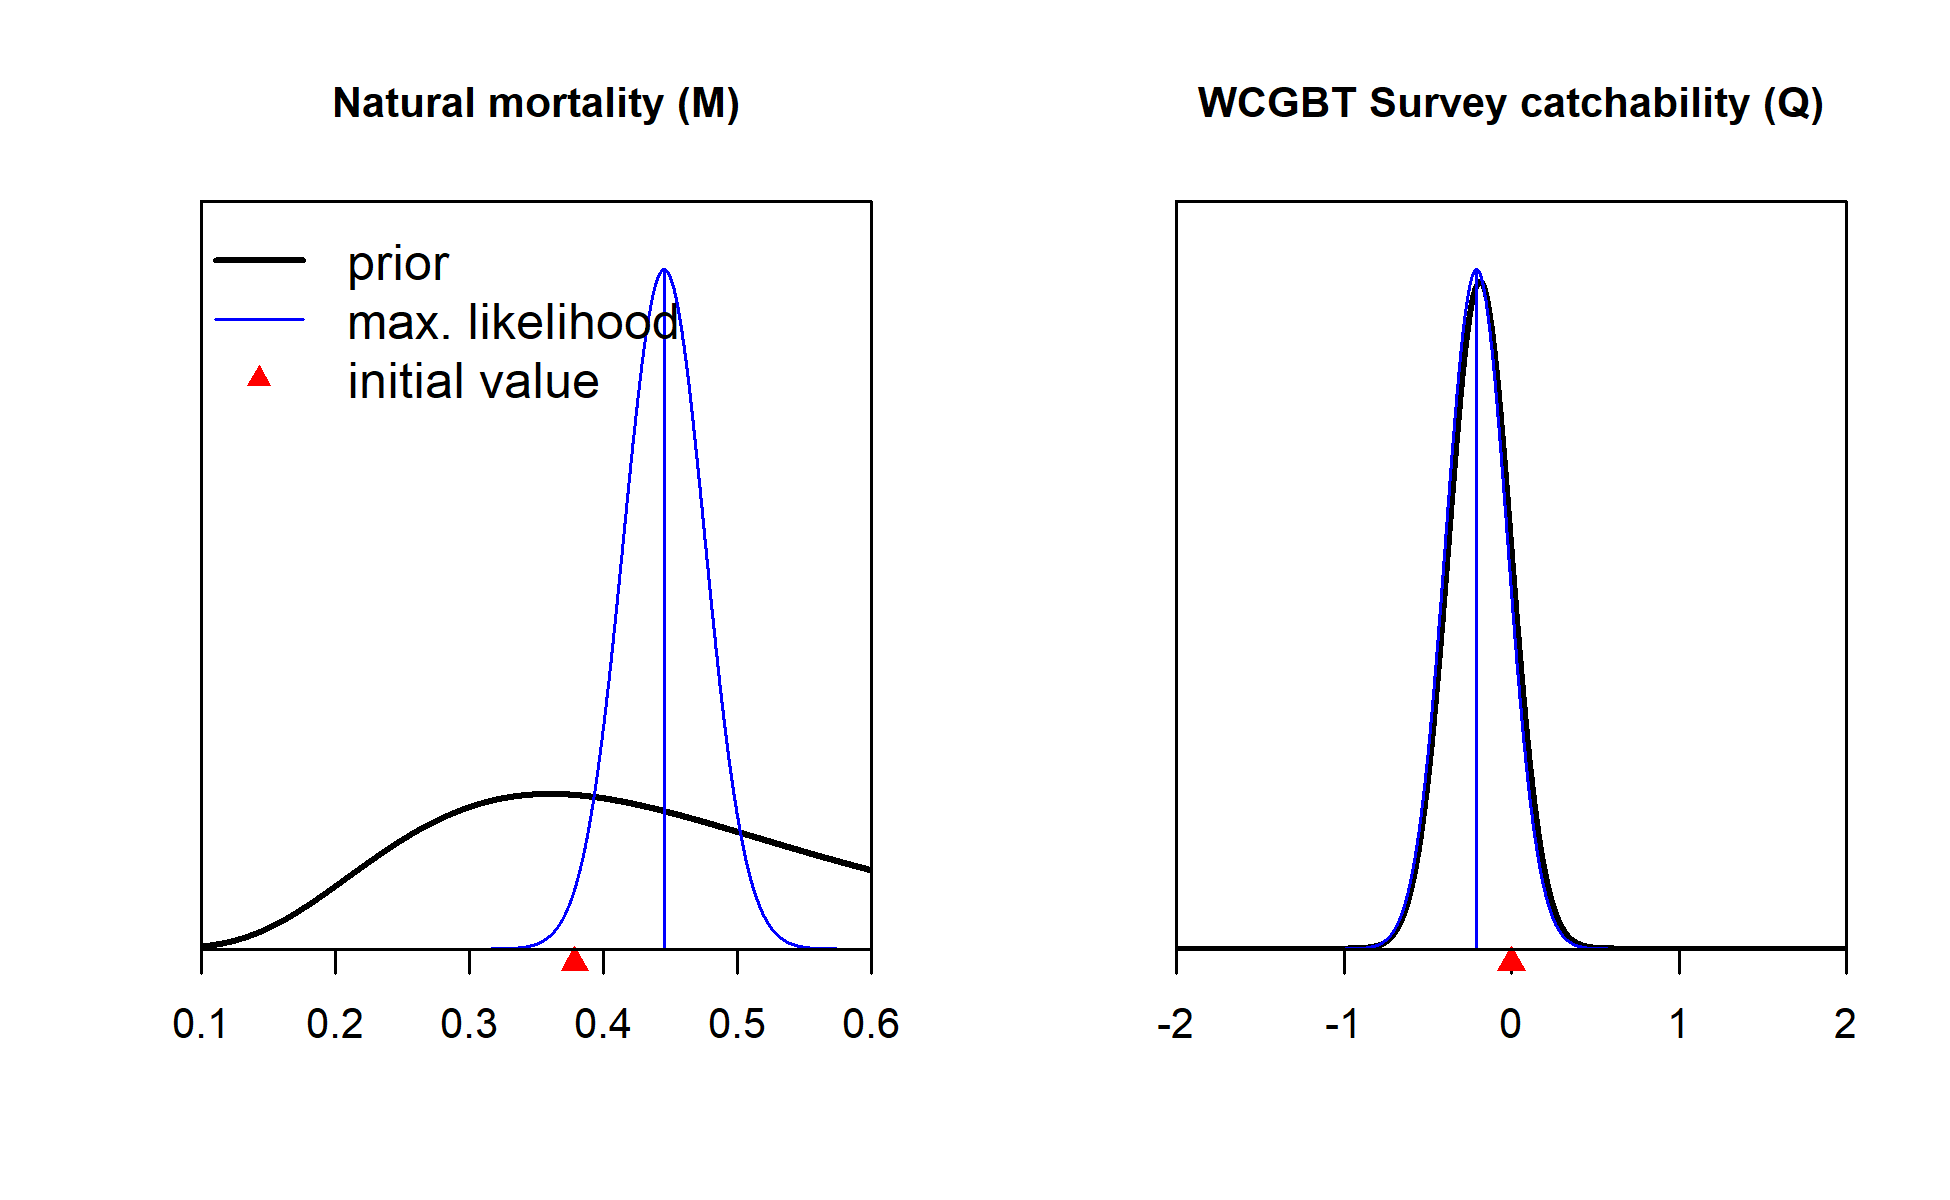
\includegraphics{Figures/fit_to_priors.png}
\caption{Estimates of natural morality and catchability of the WCGBT
Survey with normal approximations to their uncertainty compared to their
prior distributions. \label{fig:fit_to_priors}}
\end{figure}

\begin{figure}
\centering
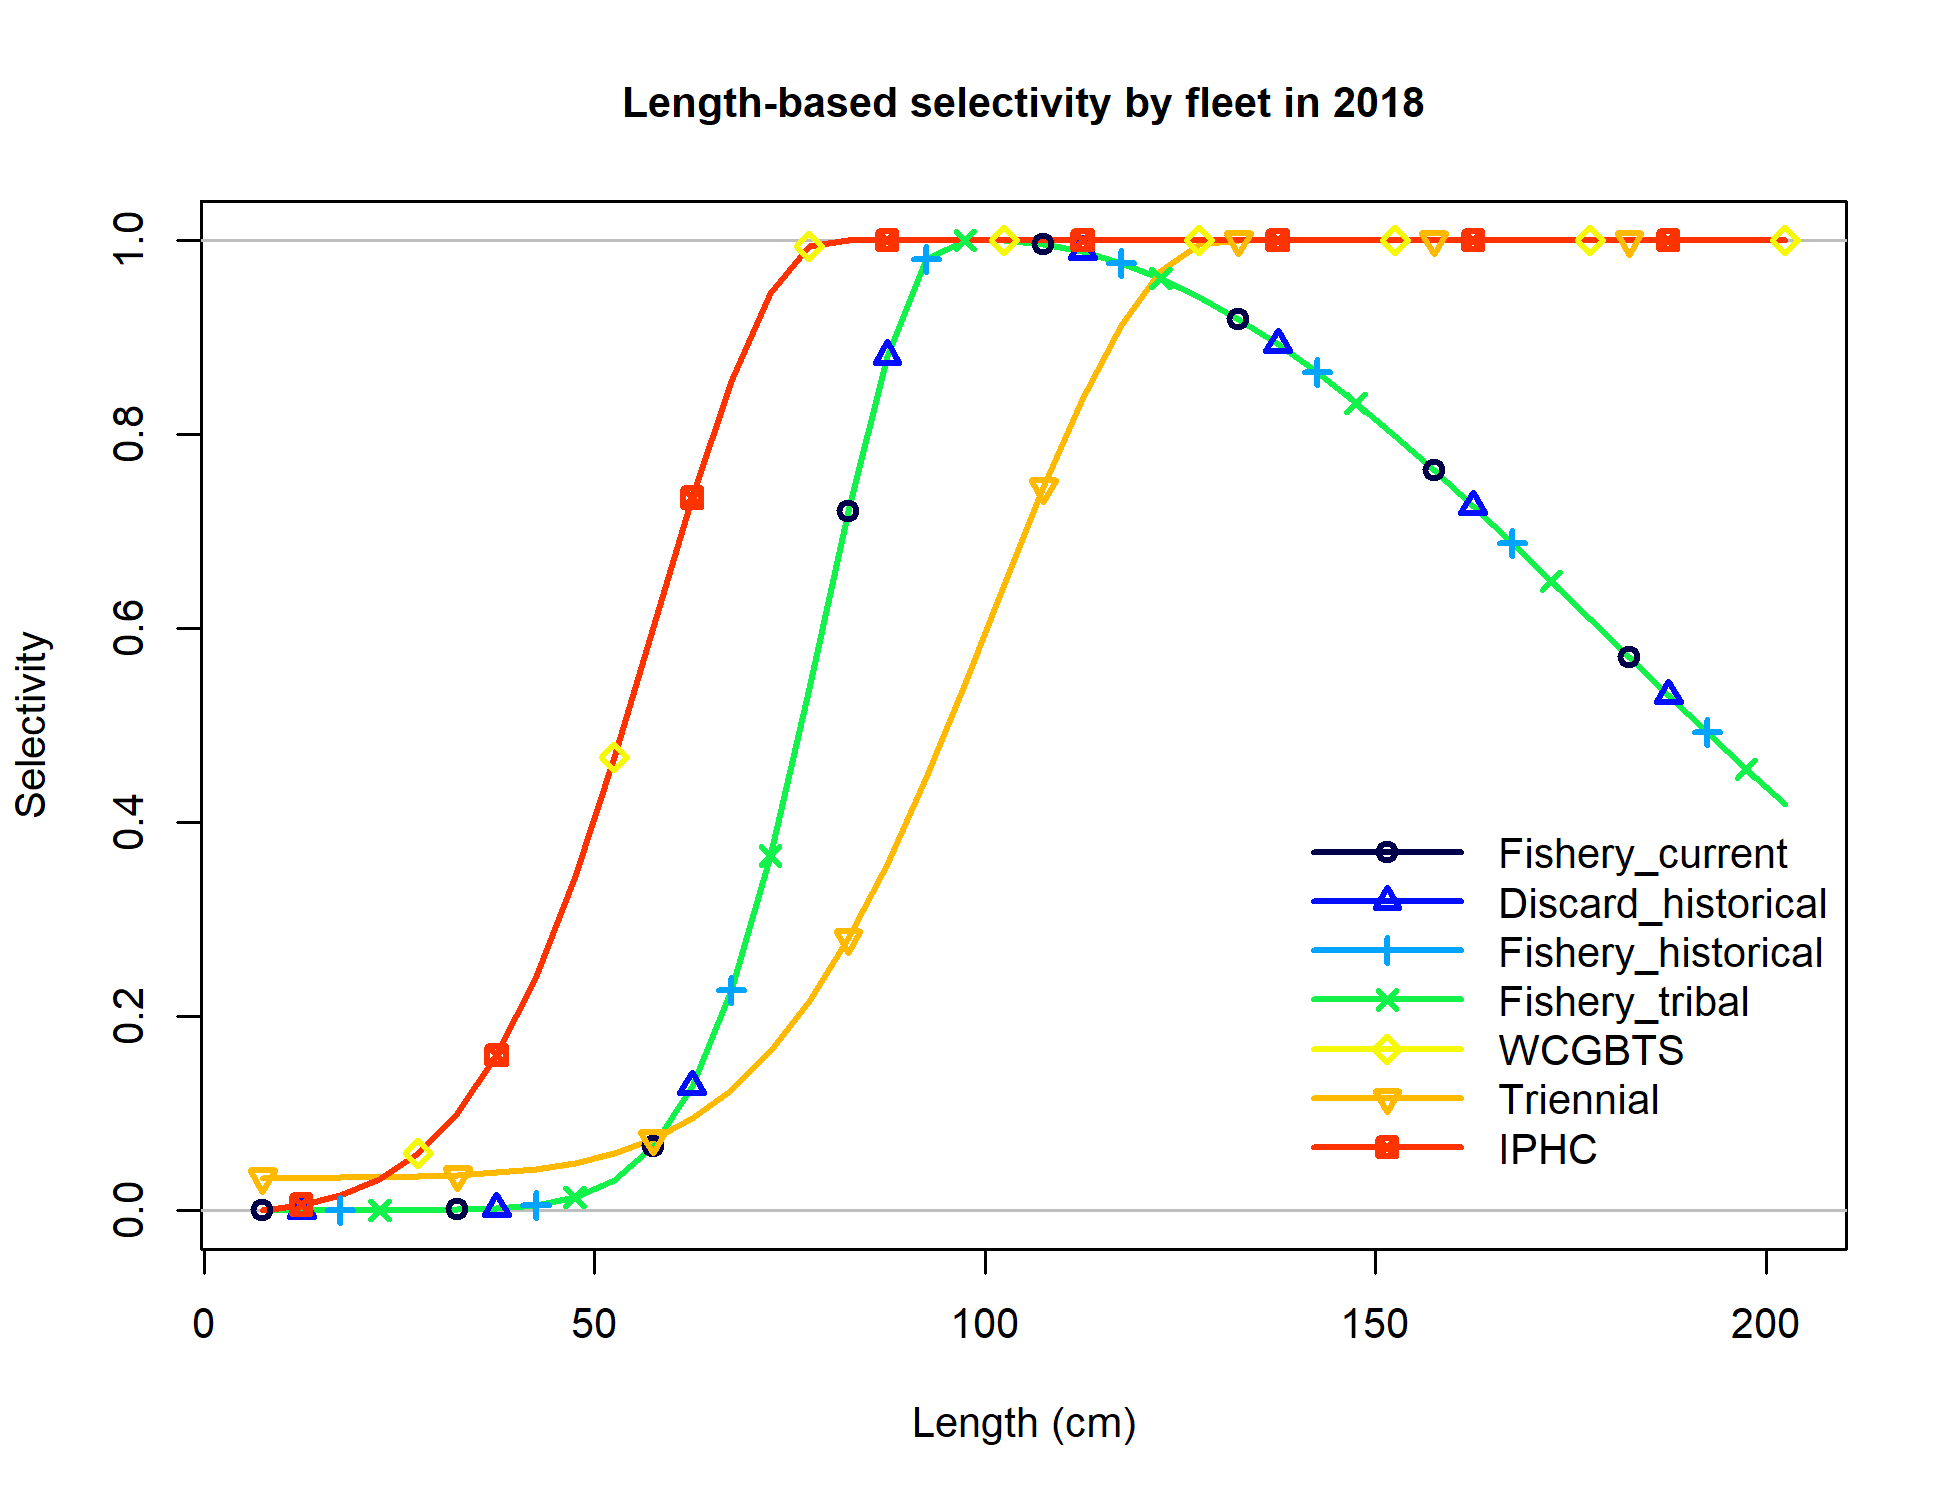
\includegraphics{r4ss/plots_mod1/sel01_multiple_fleets_length1.png}
\caption{Selectivity at length for all of the fleets in the base model.
Female selectivity is shown in the solid lines and males in the dashed
lines. \label{fig:sel01_multiple_fleets_length1}}
\end{figure}

\begin{figure}
\centering
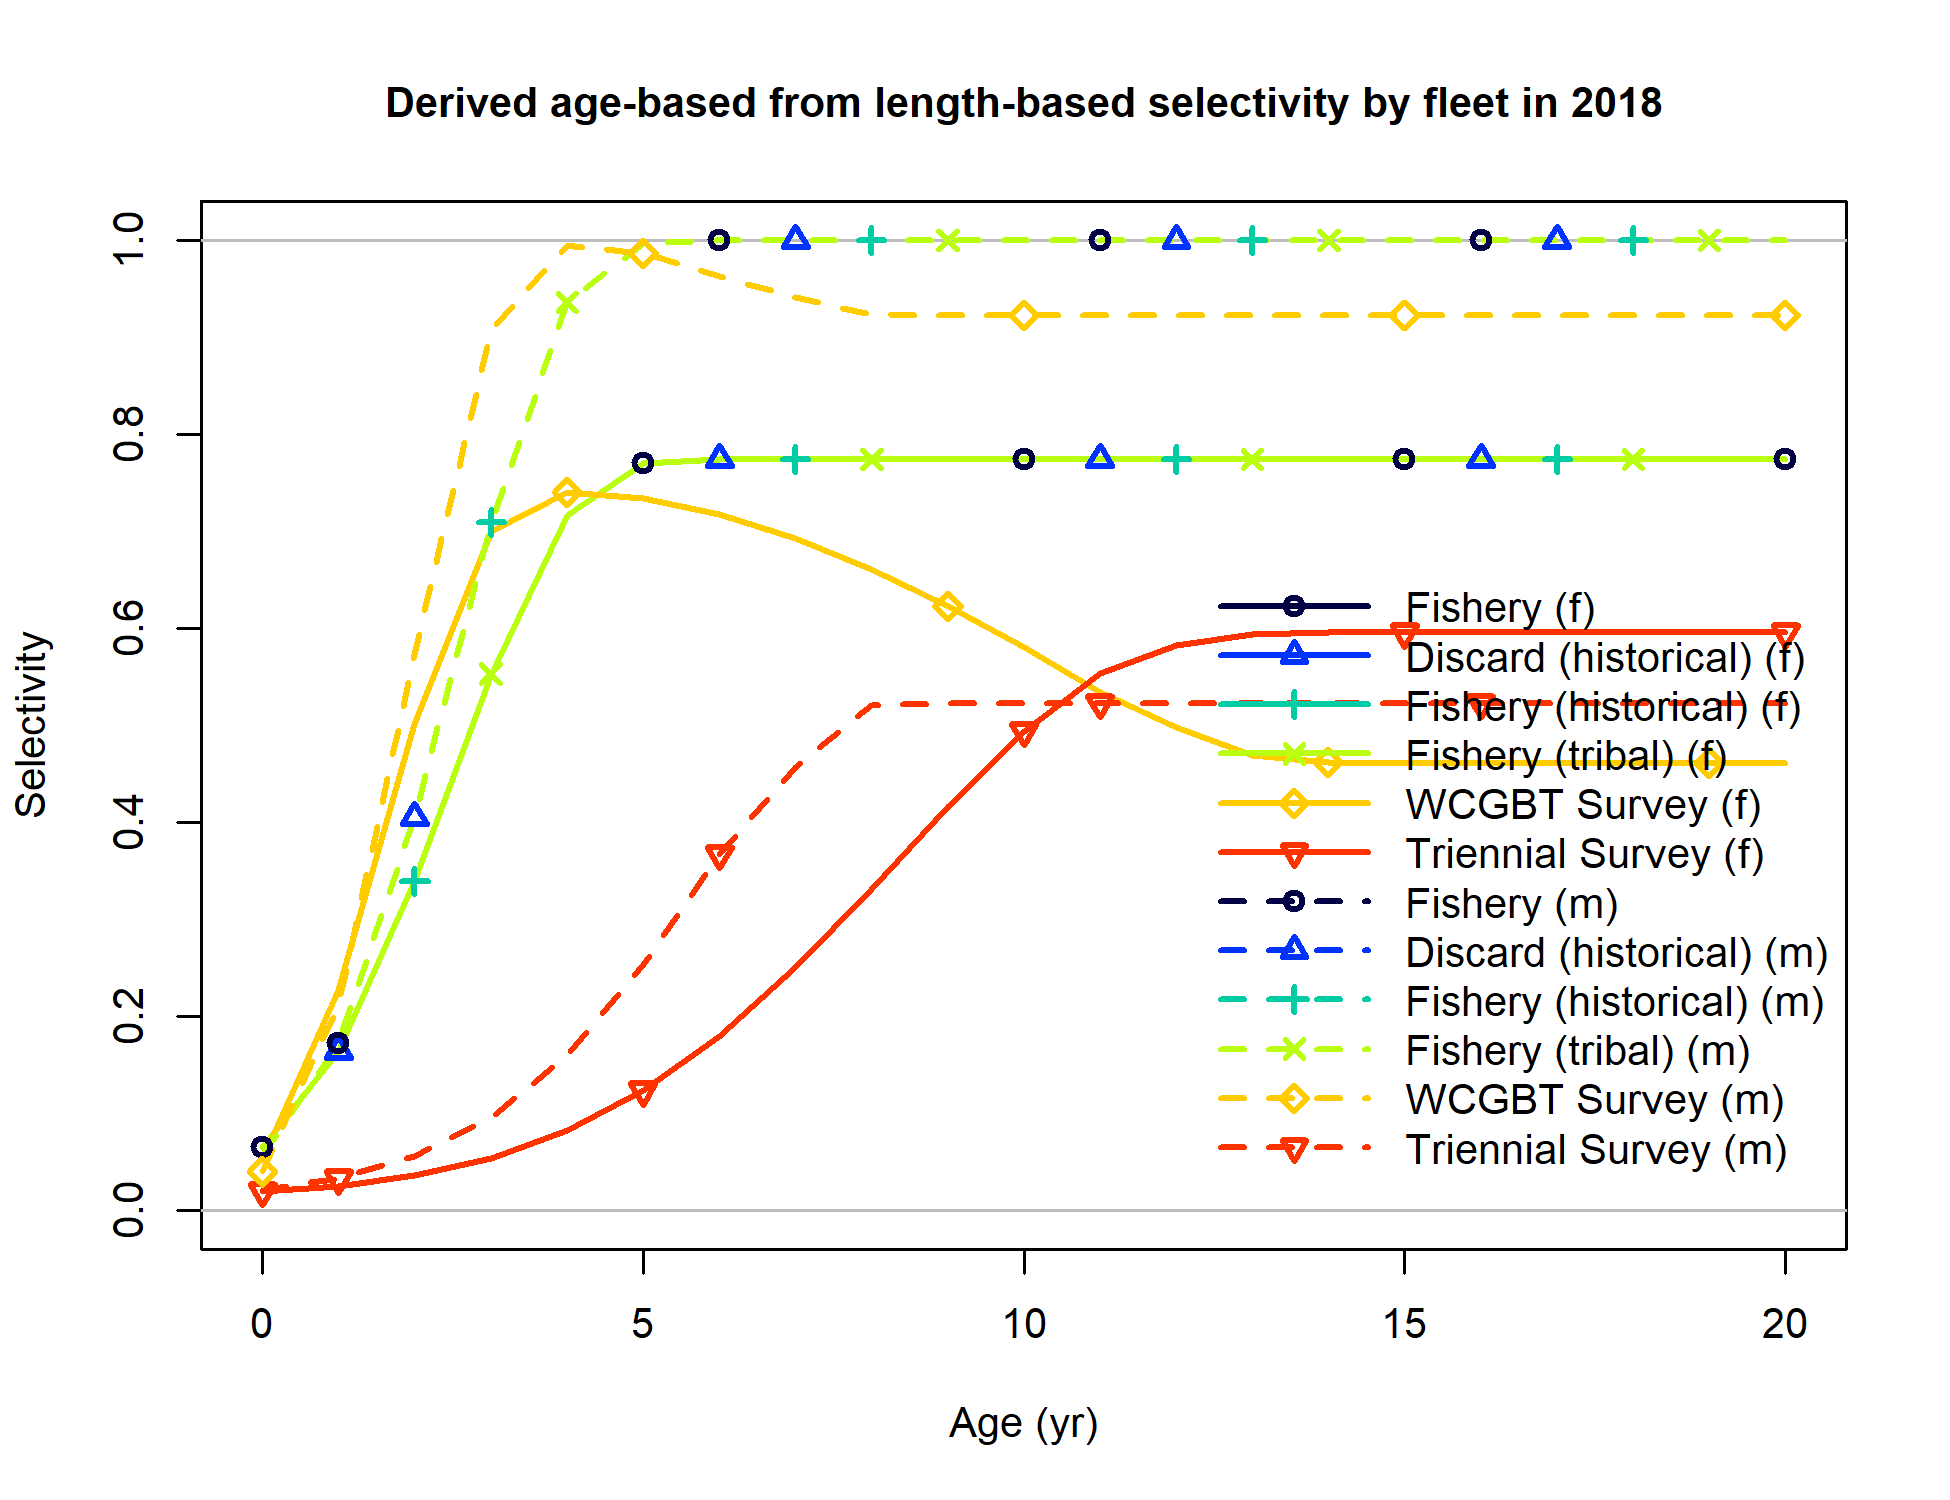
\includegraphics{r4ss/plots_mod1/sel02_multiple_fleets_age2.png}
\caption{Selectivity at age derived from the combination of
selectivity-at-length (shown above) and the estimated distribution of
length at each age for all of the fleets in the base model. Female
selectivity is shown in the solid lines and males in the dashed lines.
\label{fig:sel02_multiple_fleets_age2}}
\end{figure}

\begin{figure}
\centering
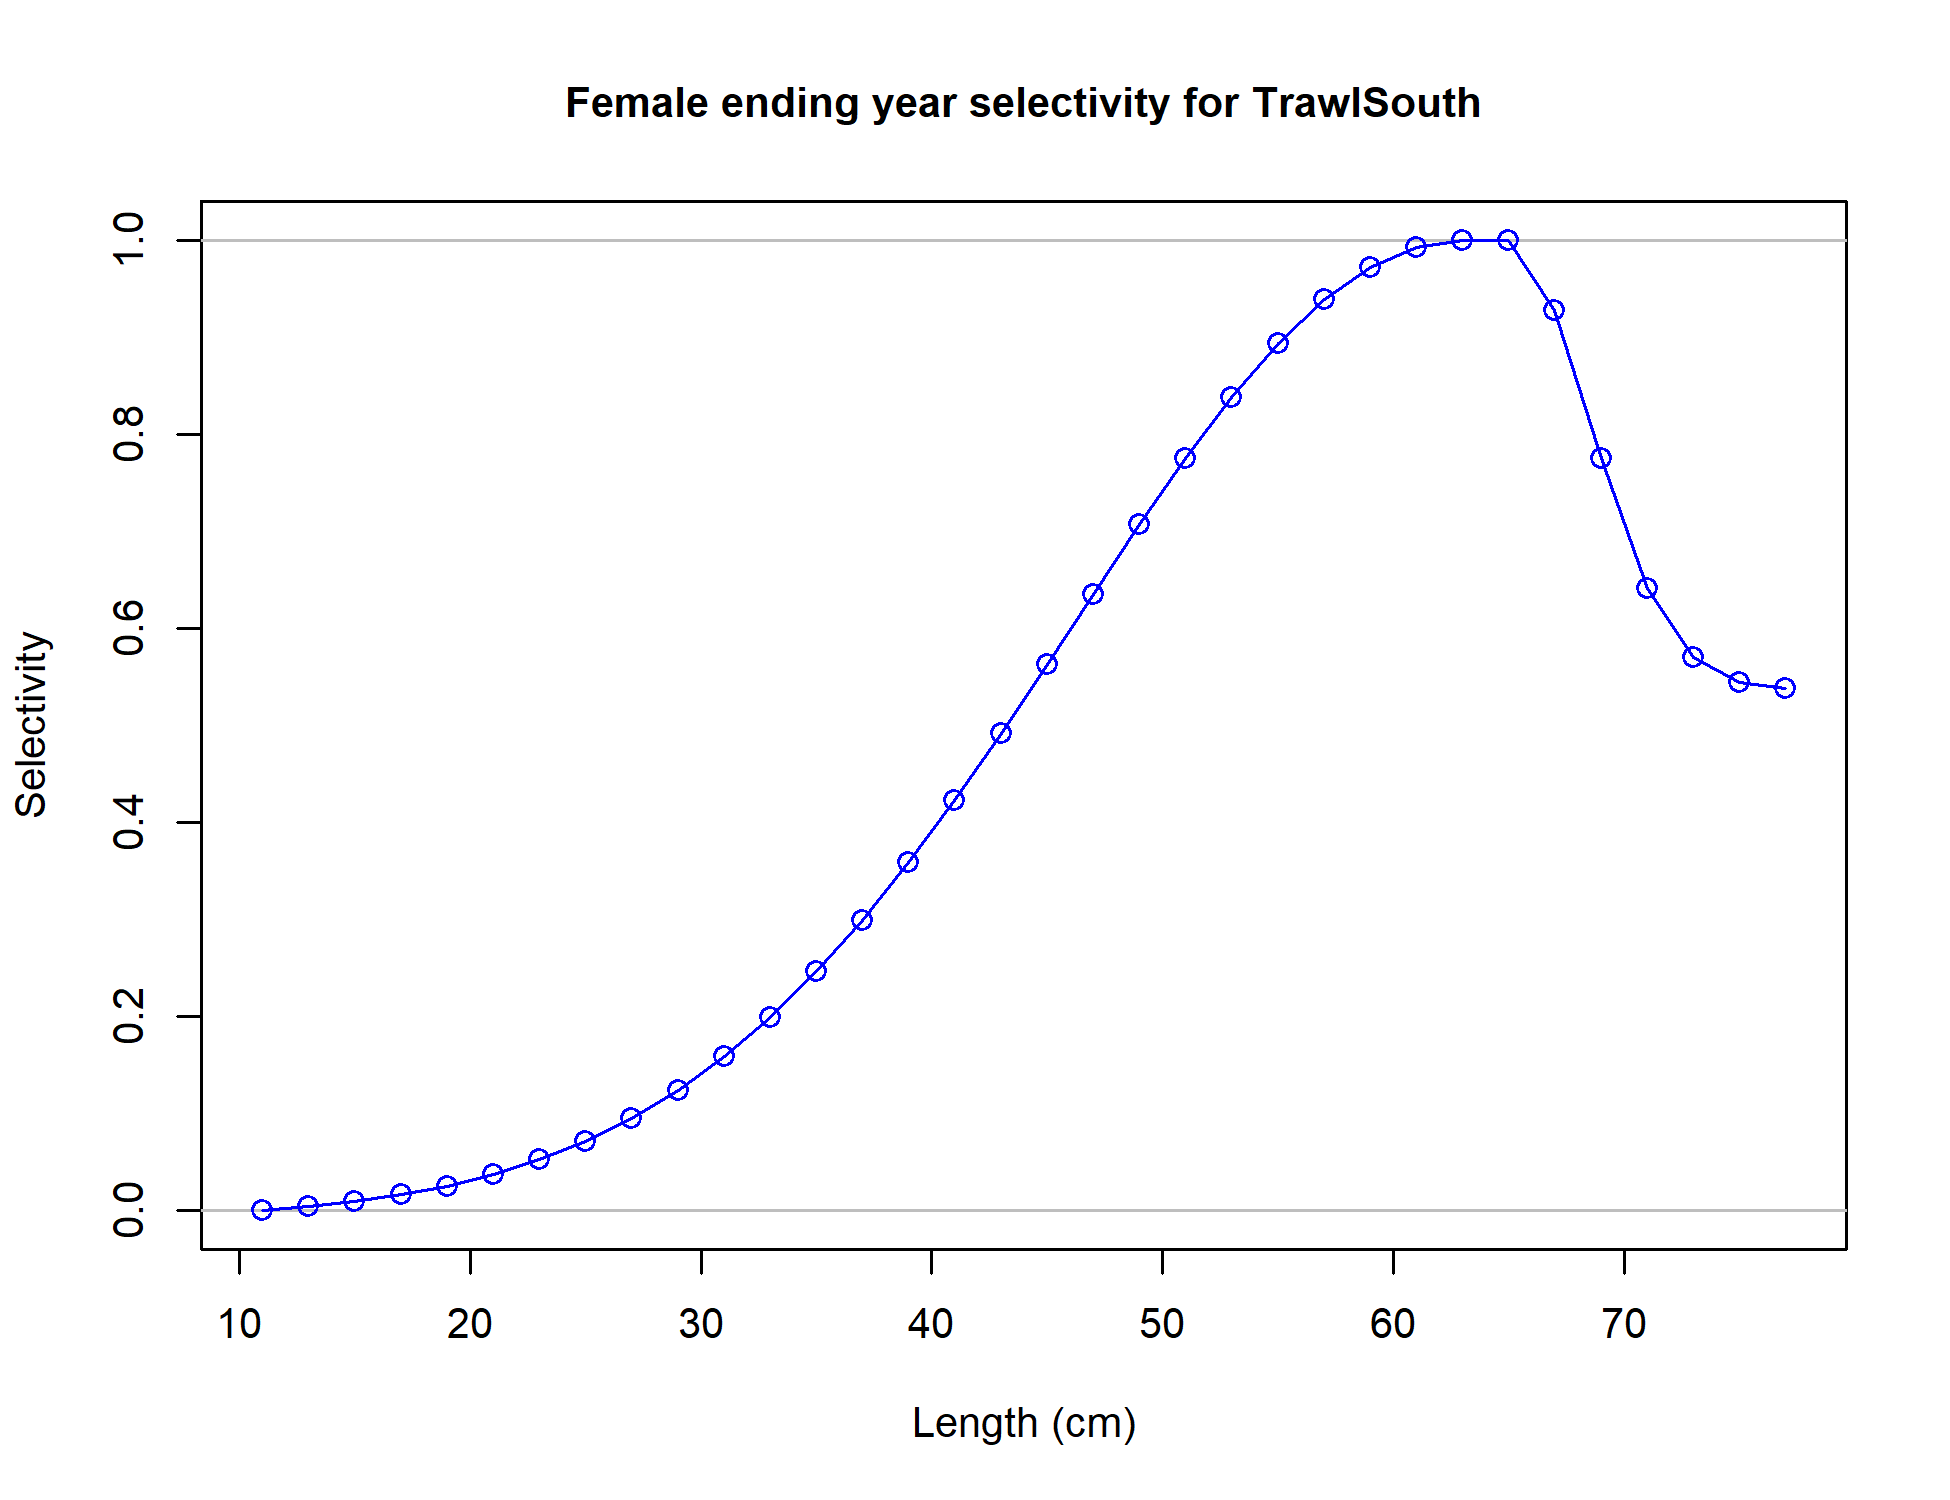
\includegraphics{r4ss/plots_mod1/sel09_len_flt1sex1.png}
\caption{Female fishery selectivity and retention in 2018 with
associated derived quantities. \label{fig:sel09_len_flt1sex1}}
\end{figure}

\begin{figure}
\centering
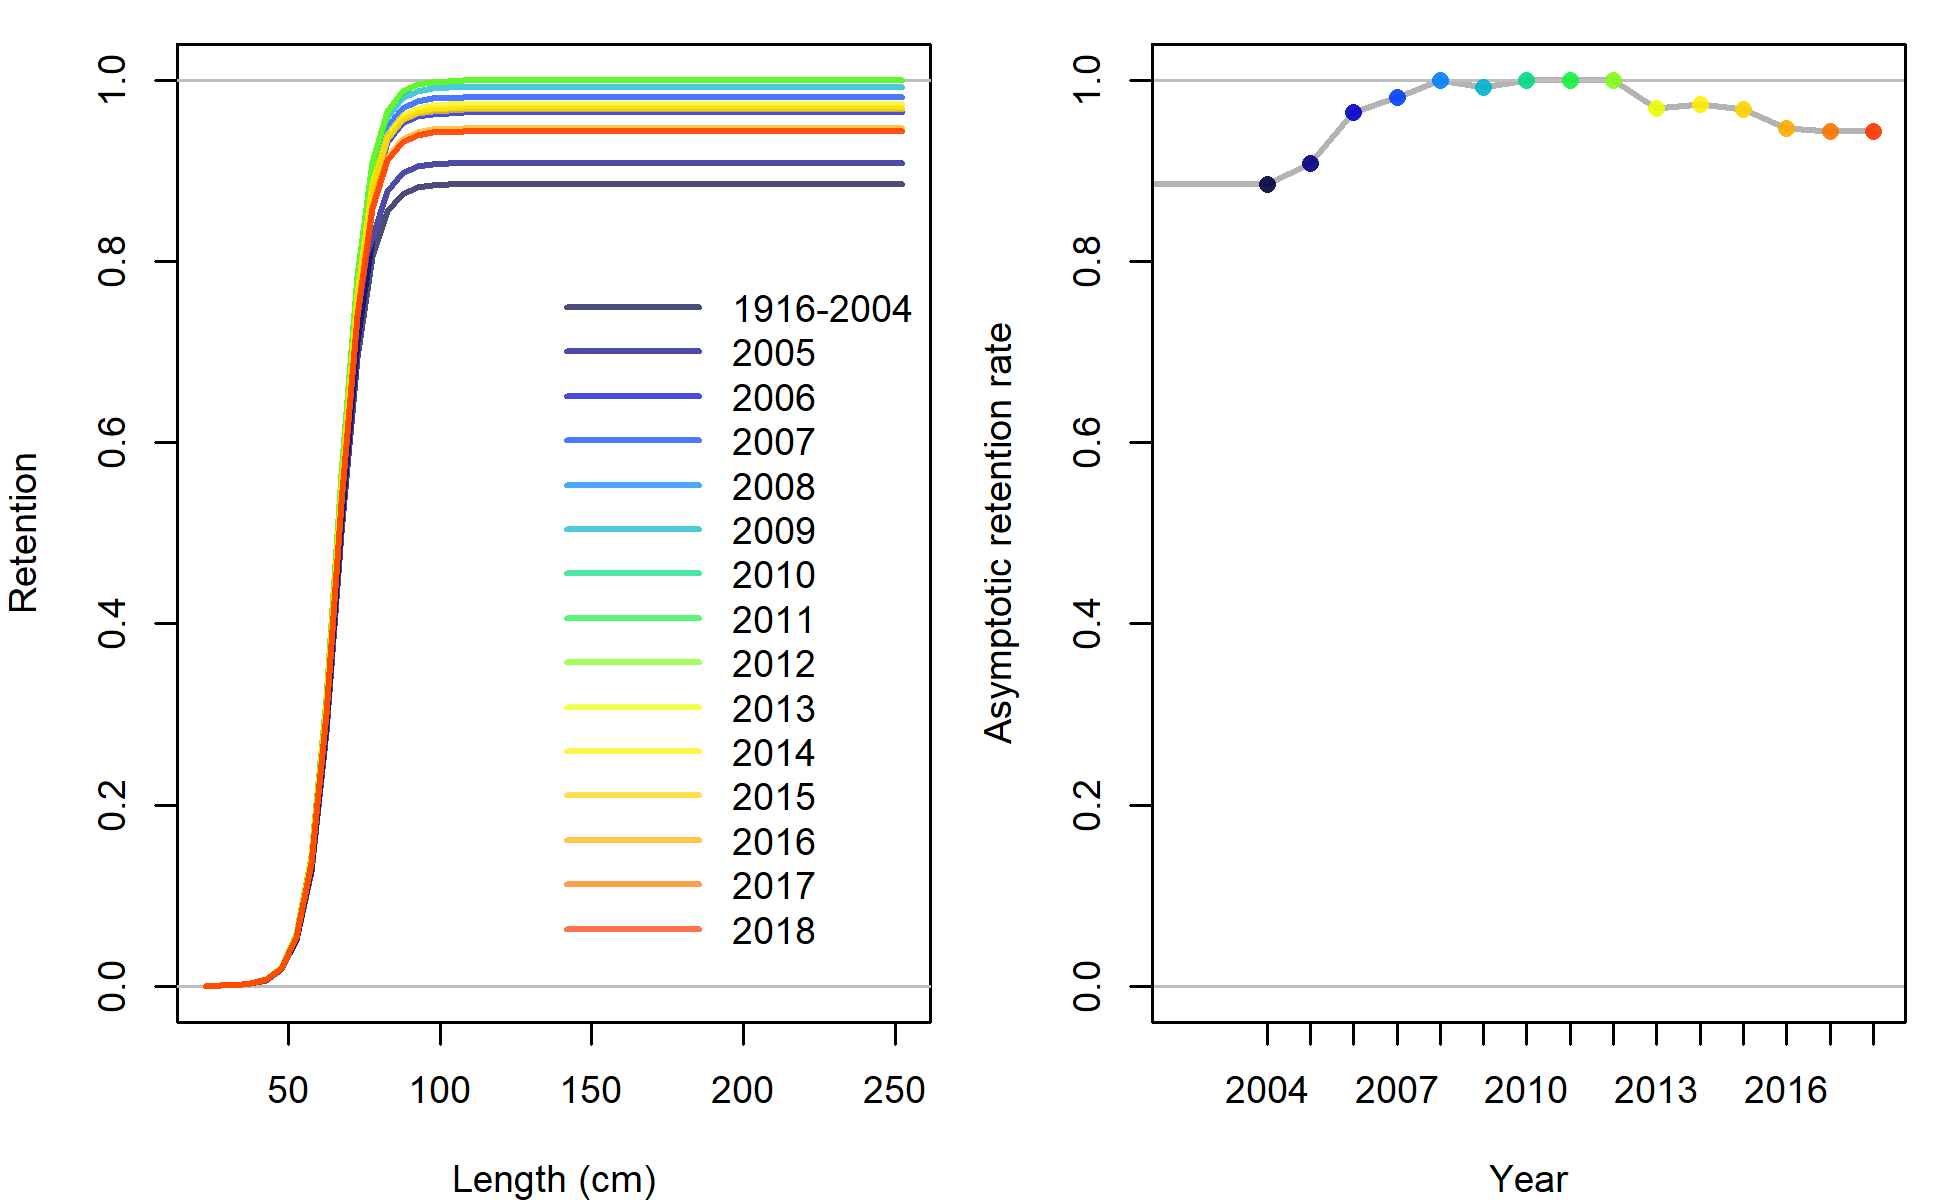
\includegraphics{Figures/retention.png}
\caption{Time-varying retention for the fishery (left) with the
time-series of asymptotic retention rates (right).
\label{fig:retention}}
\end{figure}

\FloatBarrier

\hypertarget{fits-to-the-data-1}{%
\subsubsection{Fits to the Data}\label{fits-to-the-data-1}}

\FloatBarrier

\vspace{.5cm}

\begin{figure}
\centering
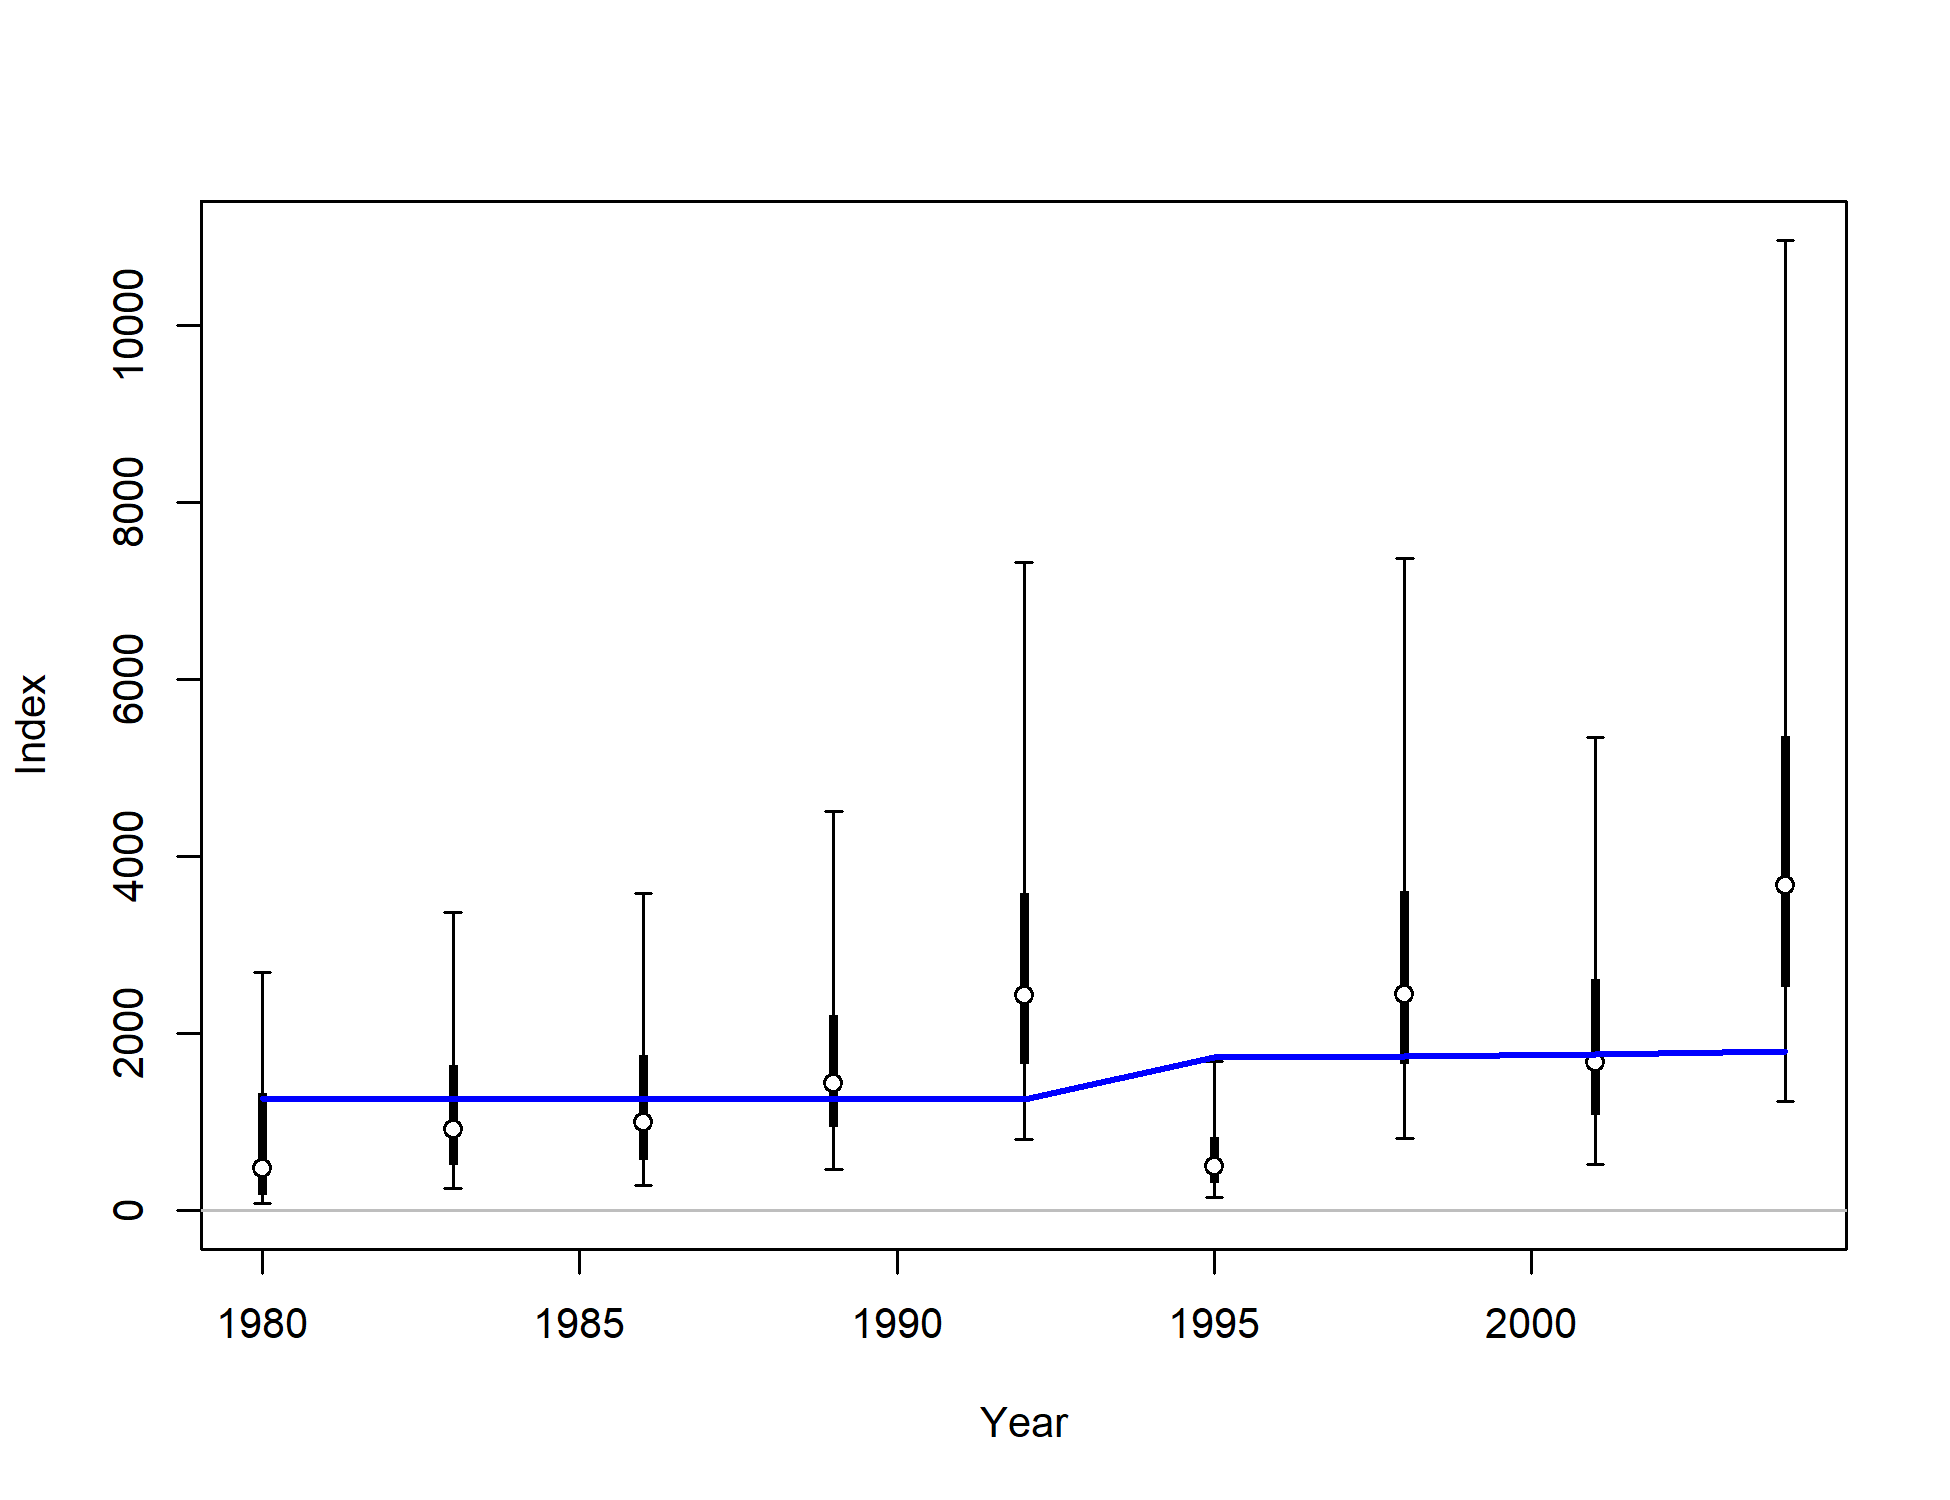
\includegraphics{r4ss/plots_mod1/index2_cpuefit_WCGBT Survey.png}
\caption{Fit to index data for WCGBT Survey. Lines indicate 95\%
uncertainty interval around index values. Thicker lines indicate input
uncertainty before addition of estimated additional uncertainty
parameter. The blue line indicates the model
estimate.\label{fig:index2_cpuefit_WCGBTS}}
\end{figure}

\begin{figure}
\centering
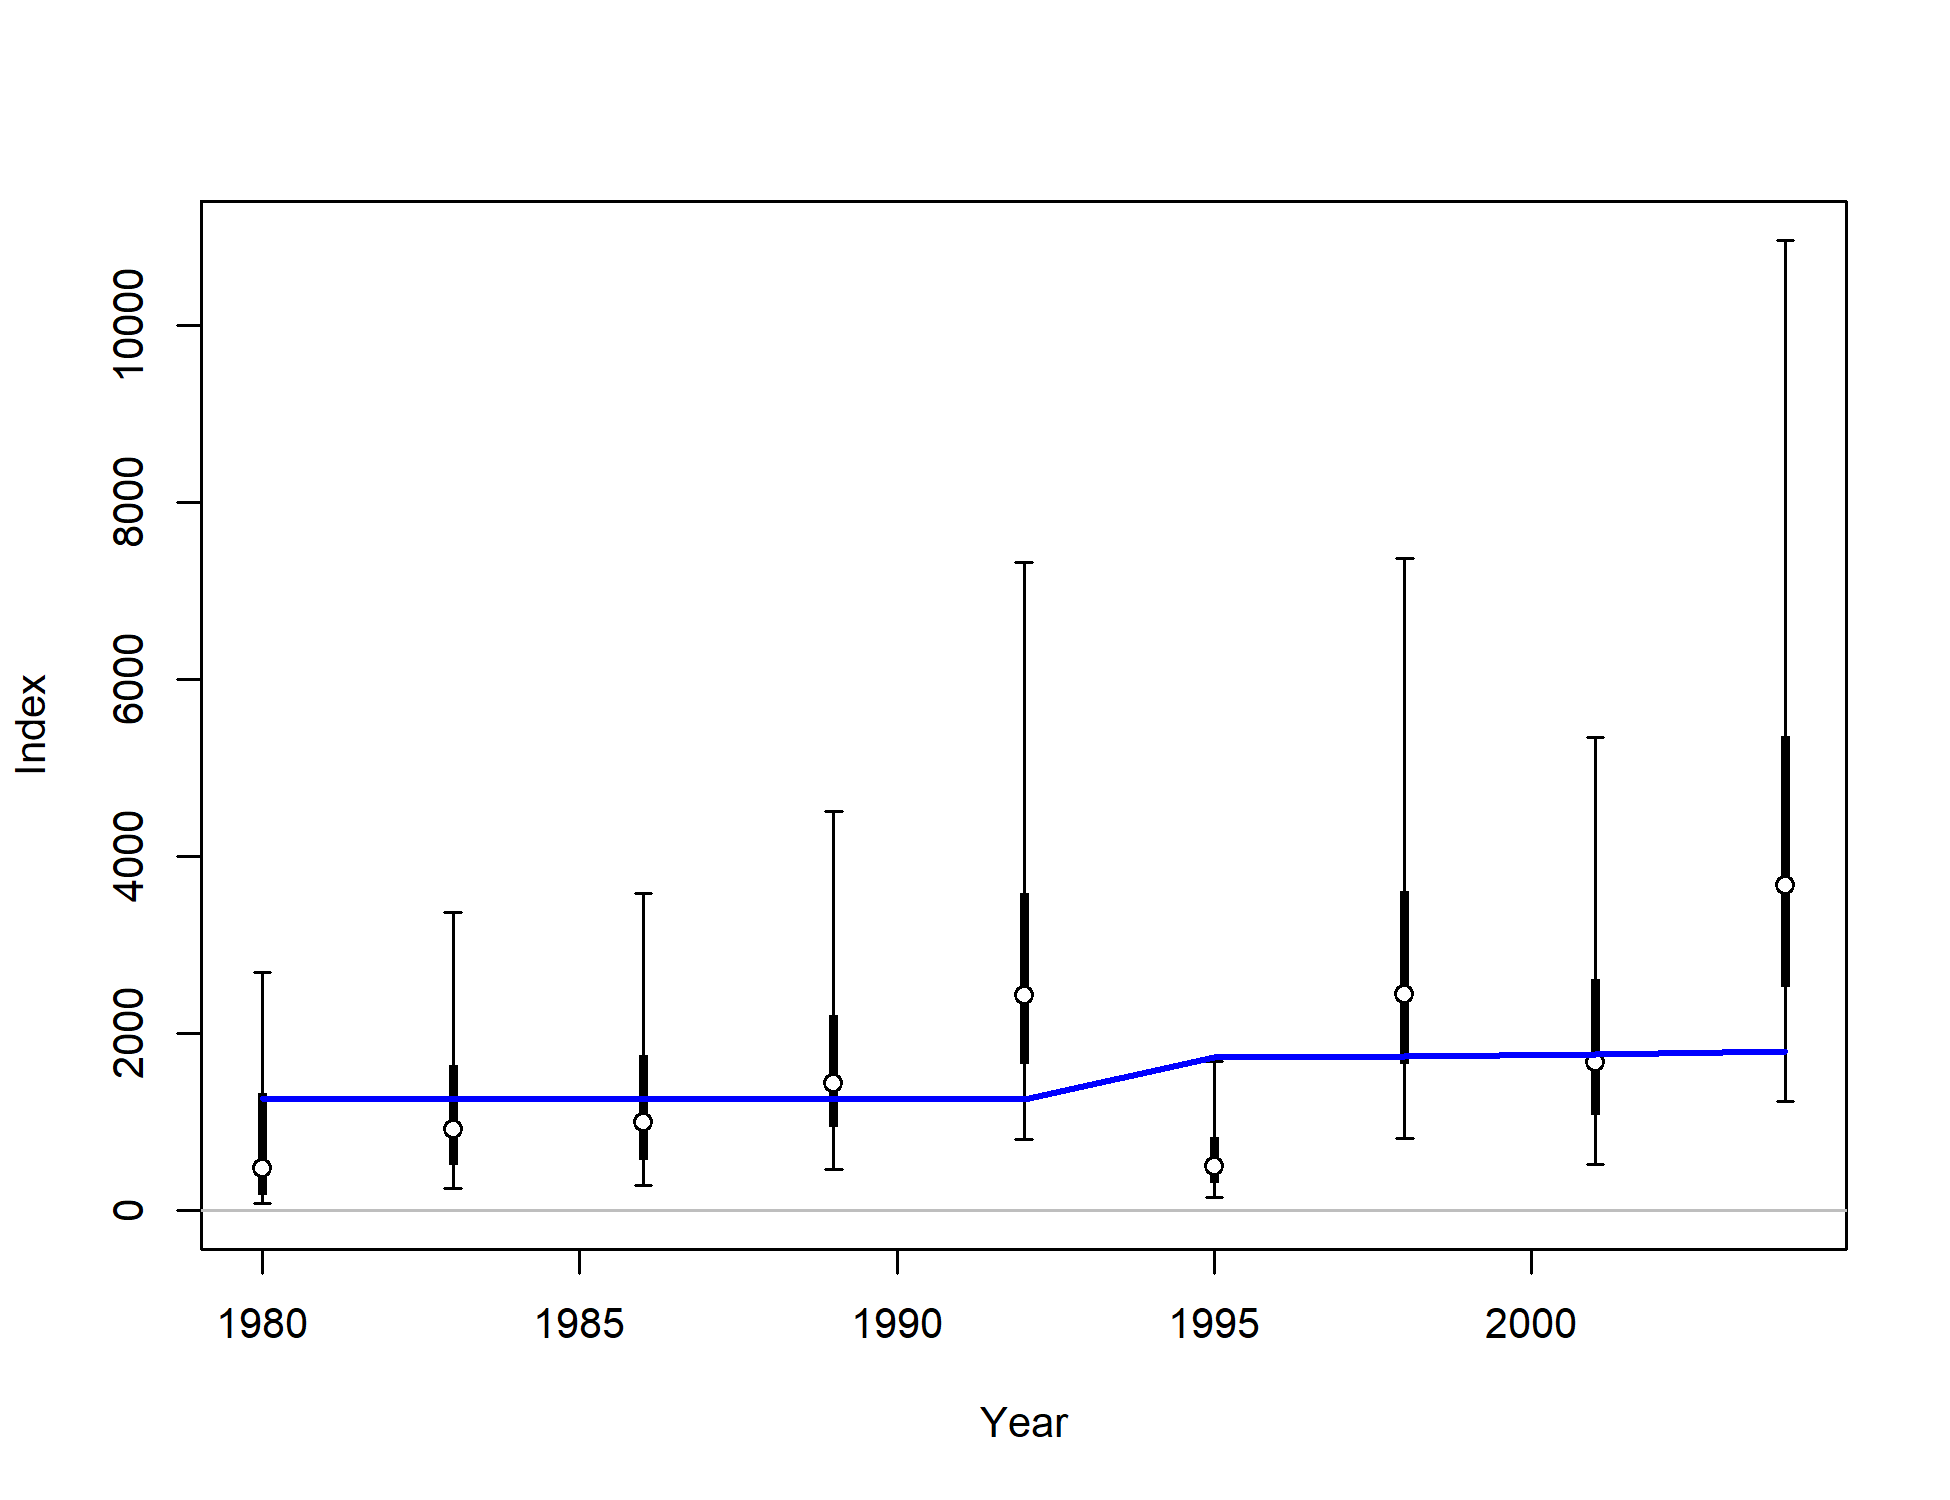
\includegraphics{r4ss/plots_mod1/index2_cpuefit_Triennial Survey.png}
\caption{Fit to index data for Triennial Survey. Lines indicate 95\%
uncertainty interval around index values. Thicker lines indicate input
uncertainty before addition of estimated additional uncertainty
parameter. The blue line indicates the model estimate with a change
between 1992 and 1995 associated with the estimated change in
catchability.\label{fig:index2_cpuefit_Triennial}}
\end{figure}

\begin{figure}
\centering
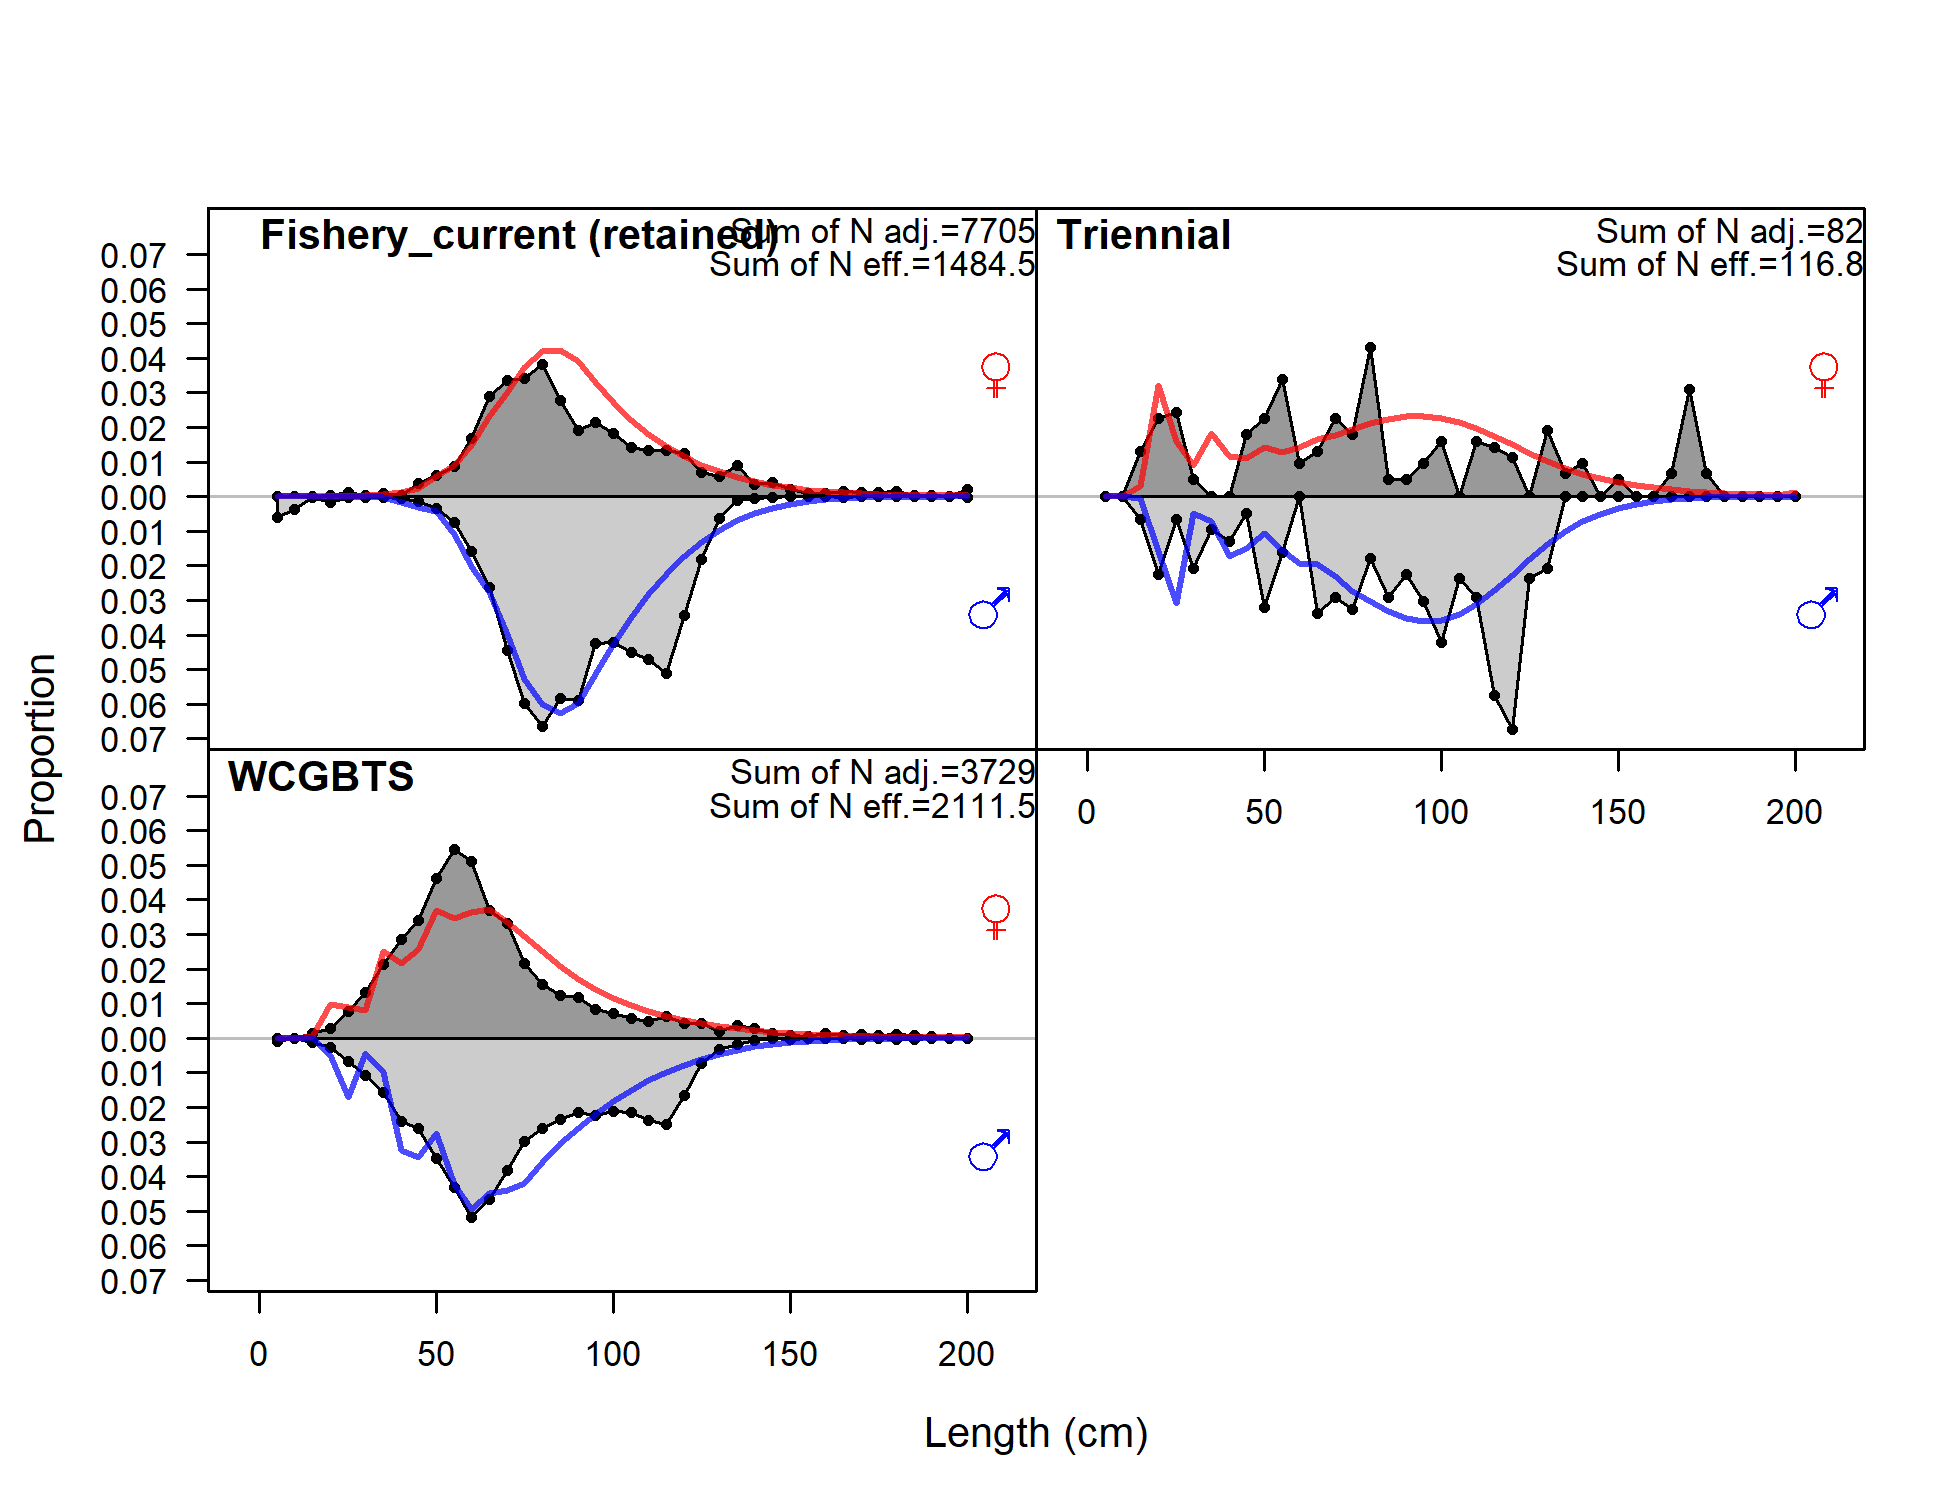
\includegraphics{r4ss/plots_mod1/comp_lenfit__aggregated_across_time.png}
\caption{Fits to length comp data, aggregated across time by fleet.
\label{fig:comp_lenfit_aggregated_across_time}}
\end{figure}

\begin{figure}
\centering
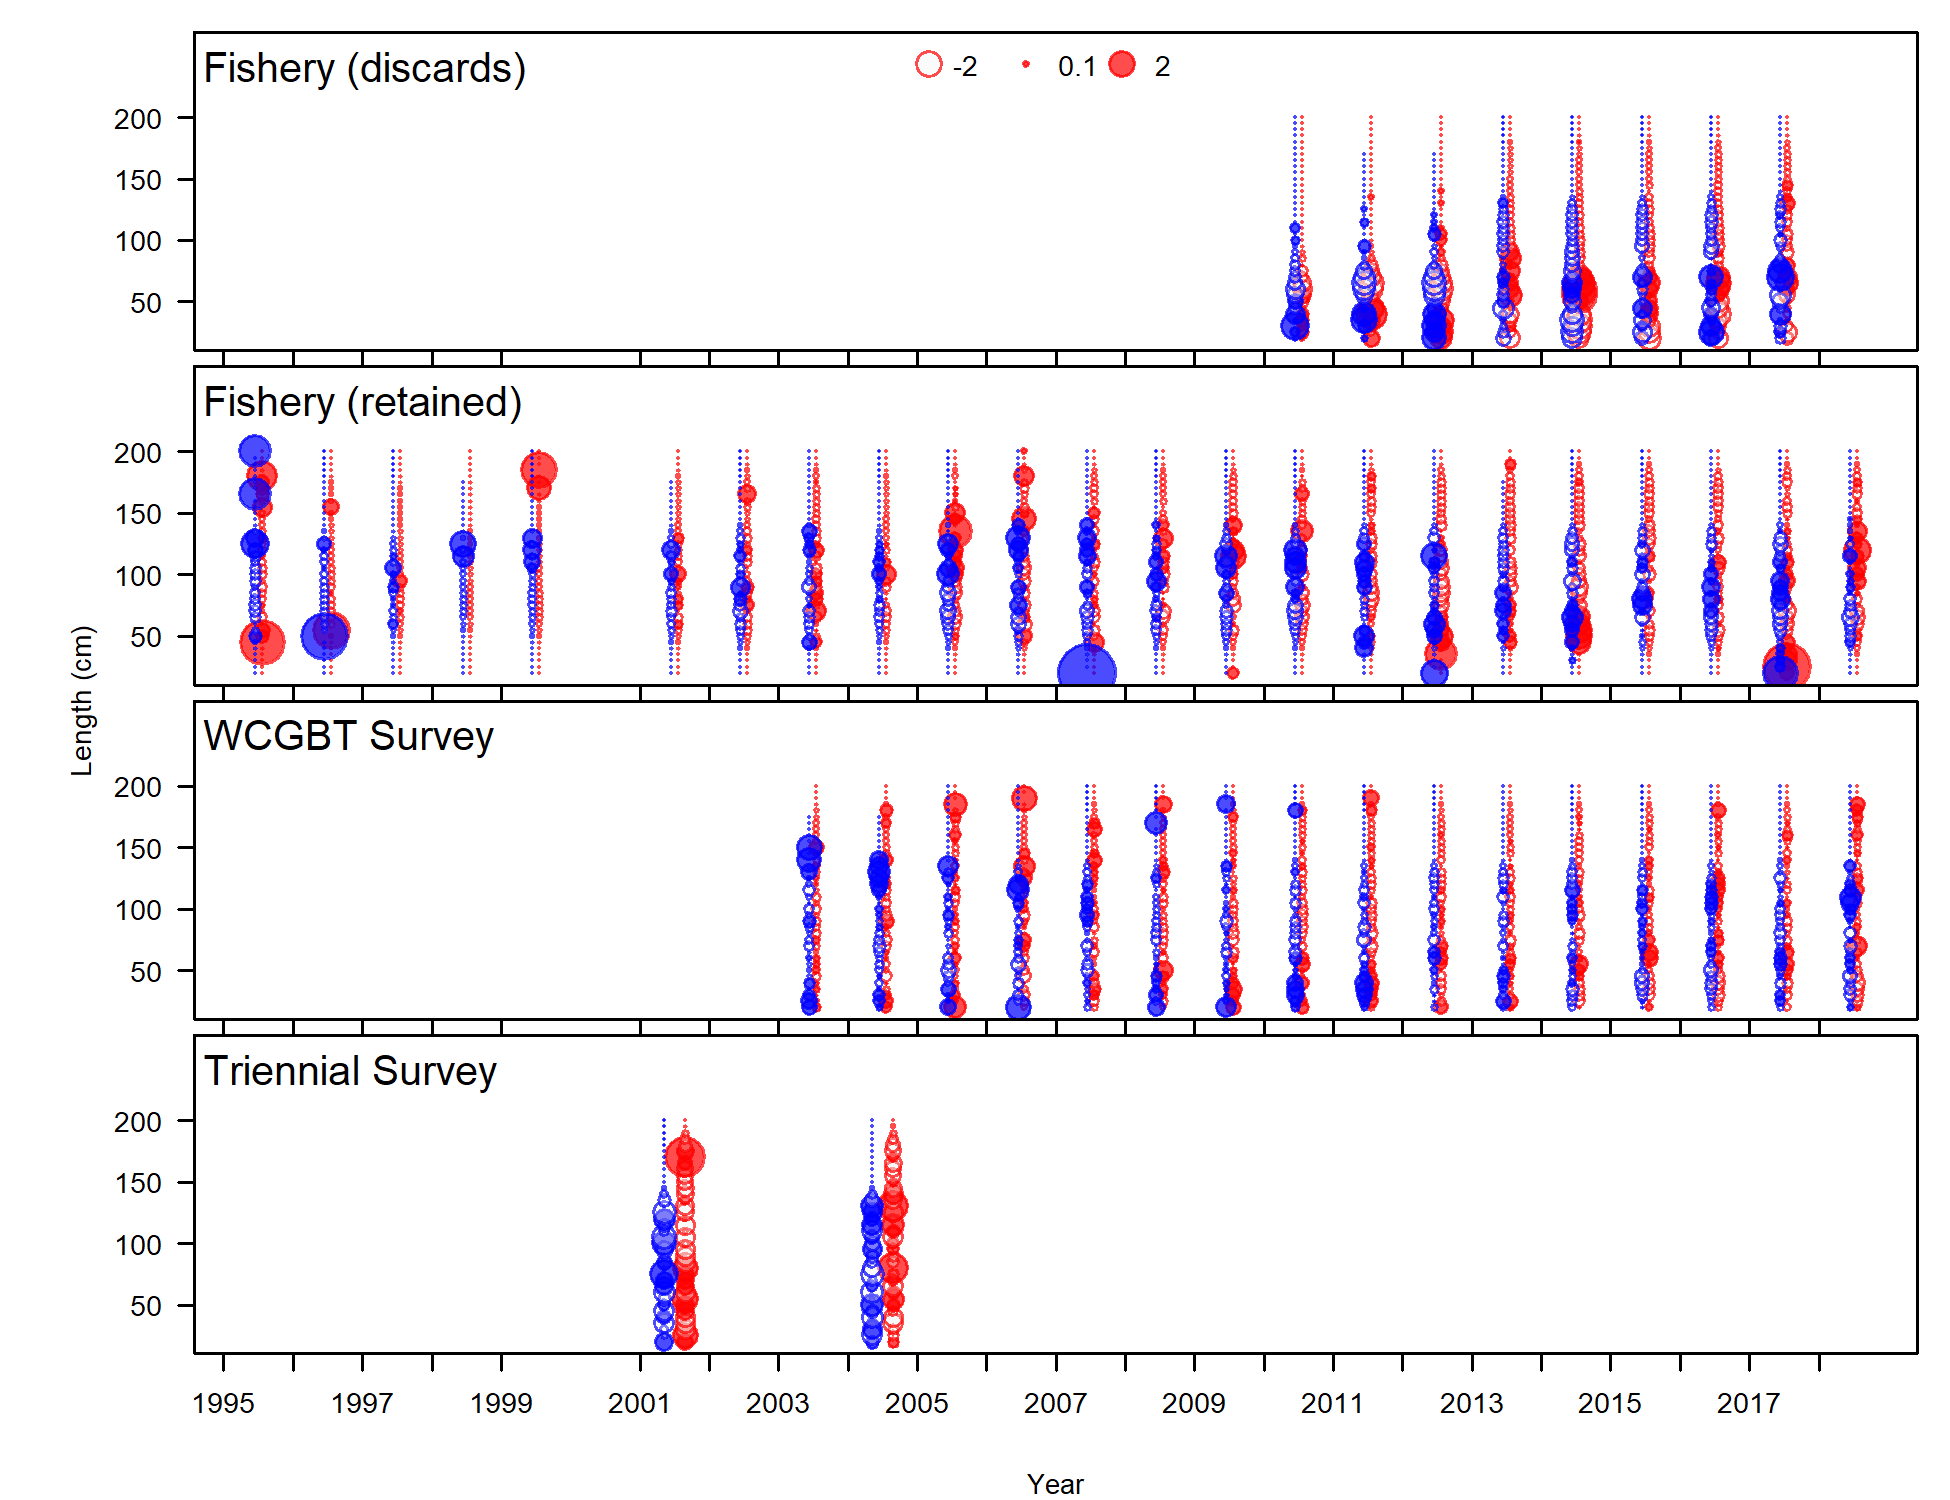
\includegraphics{r4ss/plots_mod1/comp_lenfit__multi-fleet_comparison.png}
\caption{Pearson residuals for length composition data for all years and
fleets, with females in red and males in blue. Closed bubbles are
positive residuals (observed \textgreater{} expected) and open bubbles
are negative residuals (observed \textless{} expected).
\label{fig:comp_lenfit__multi-fleet_comparison}}
\end{figure}

\begin{figure}
\centering
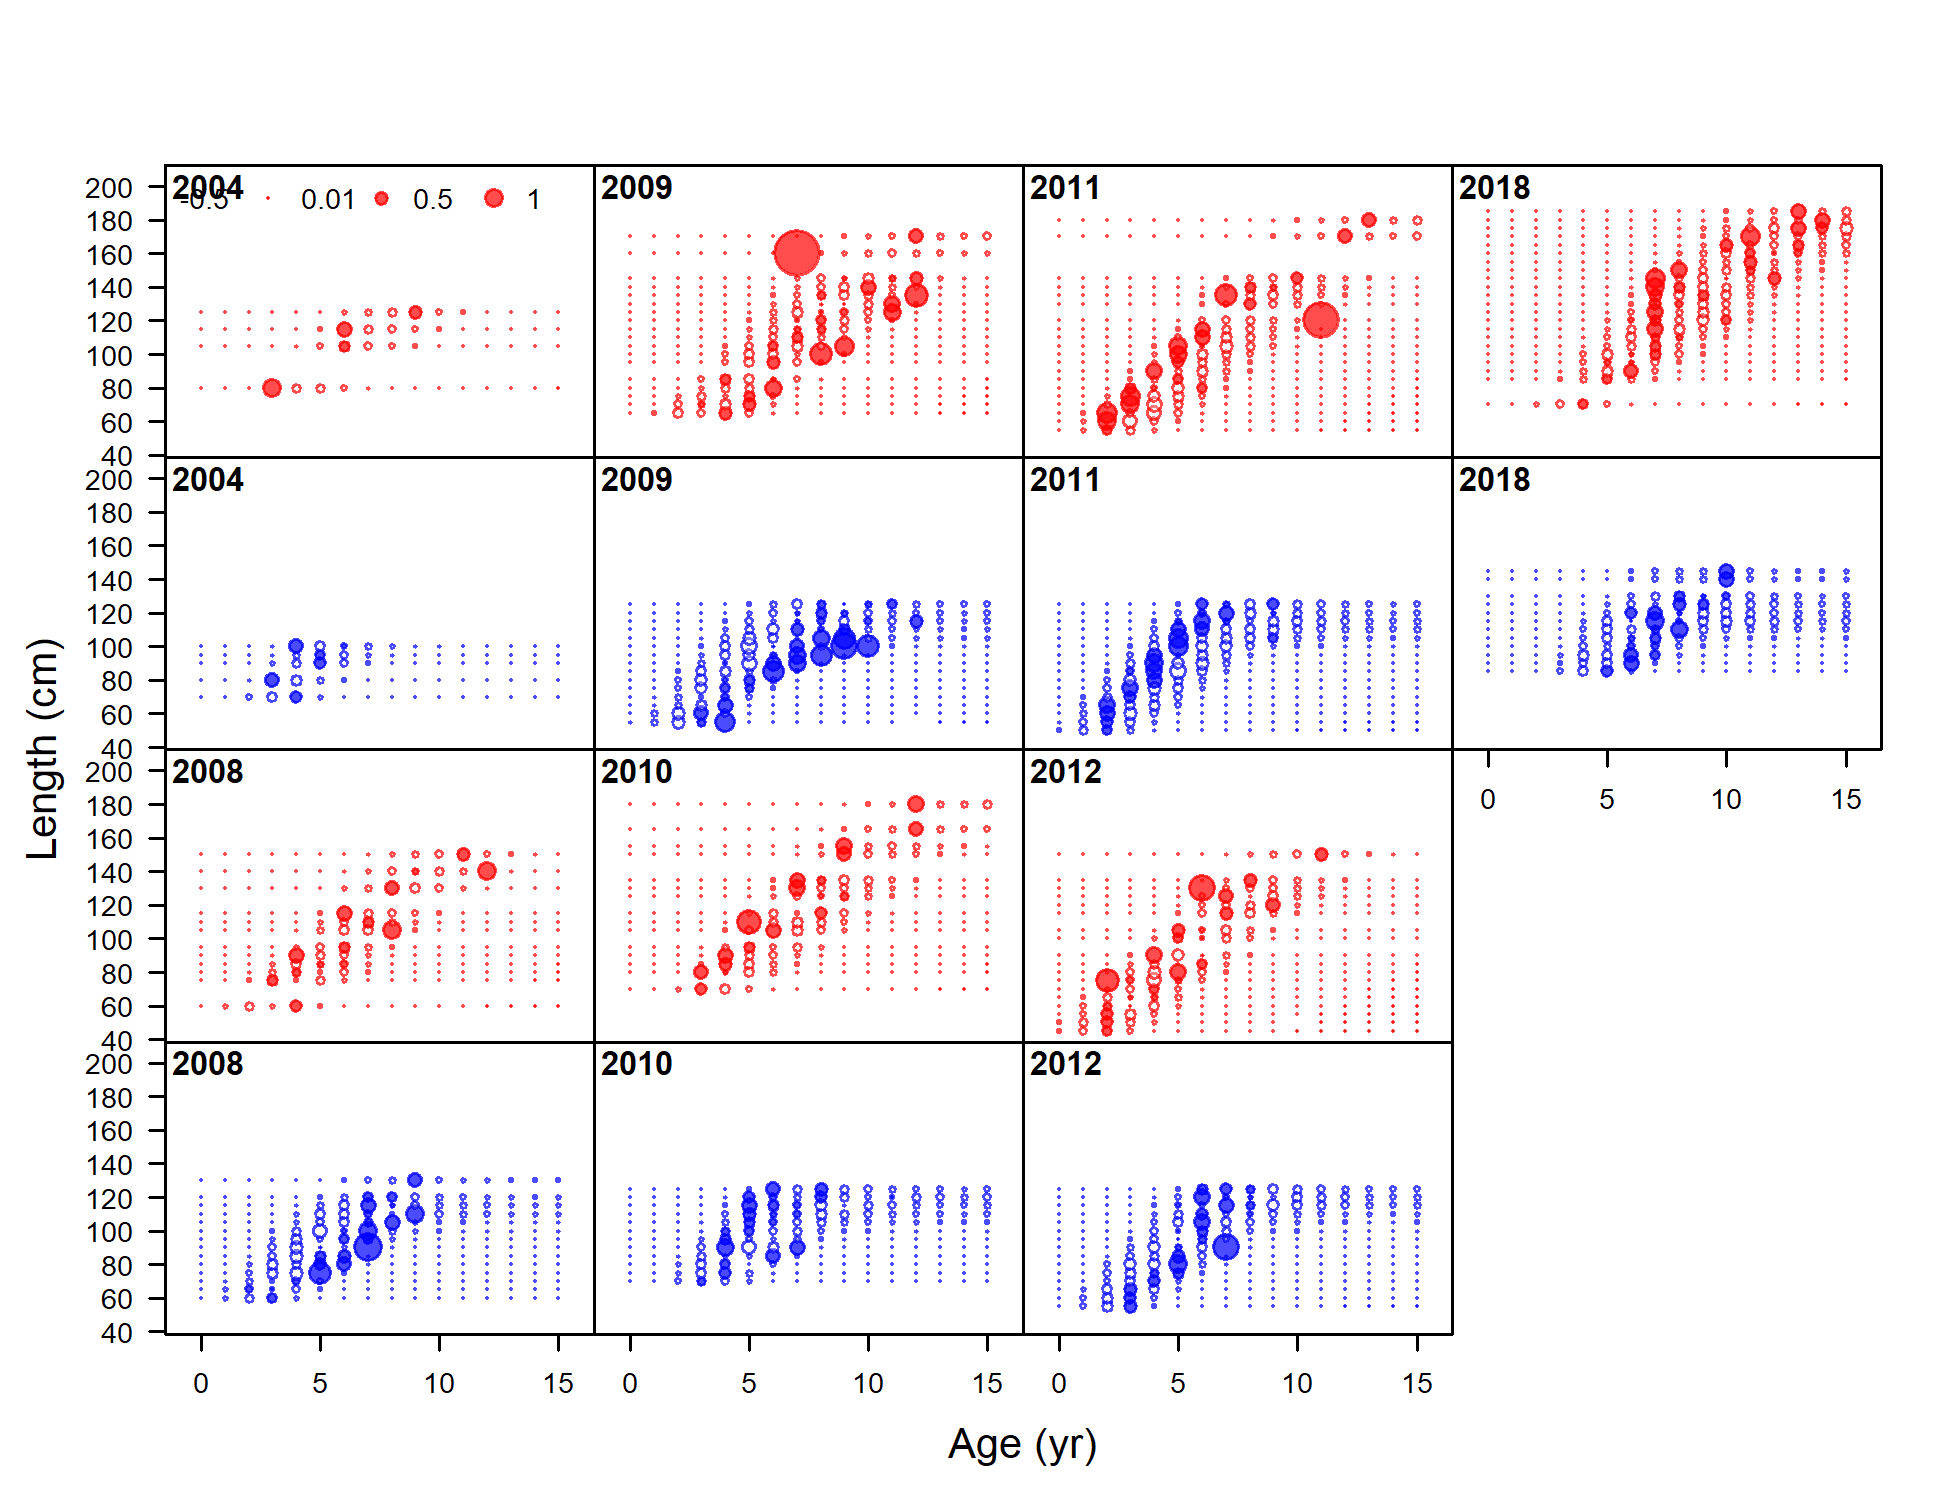
\includegraphics{r4ss/plots_mod1/comp_condAALfit_residsflt1mkt2.png}
\caption{Pearson residuals for the fit to conditional age-at-length data
from the fishery. Closed bubbles are positive residuals (observed
\textgreater{} expected) and open bubbles are negative residuals
(observed \textless{} expected). \label{fig:age_fit_fishery}}
\end{figure}

\begin{figure}
\centering
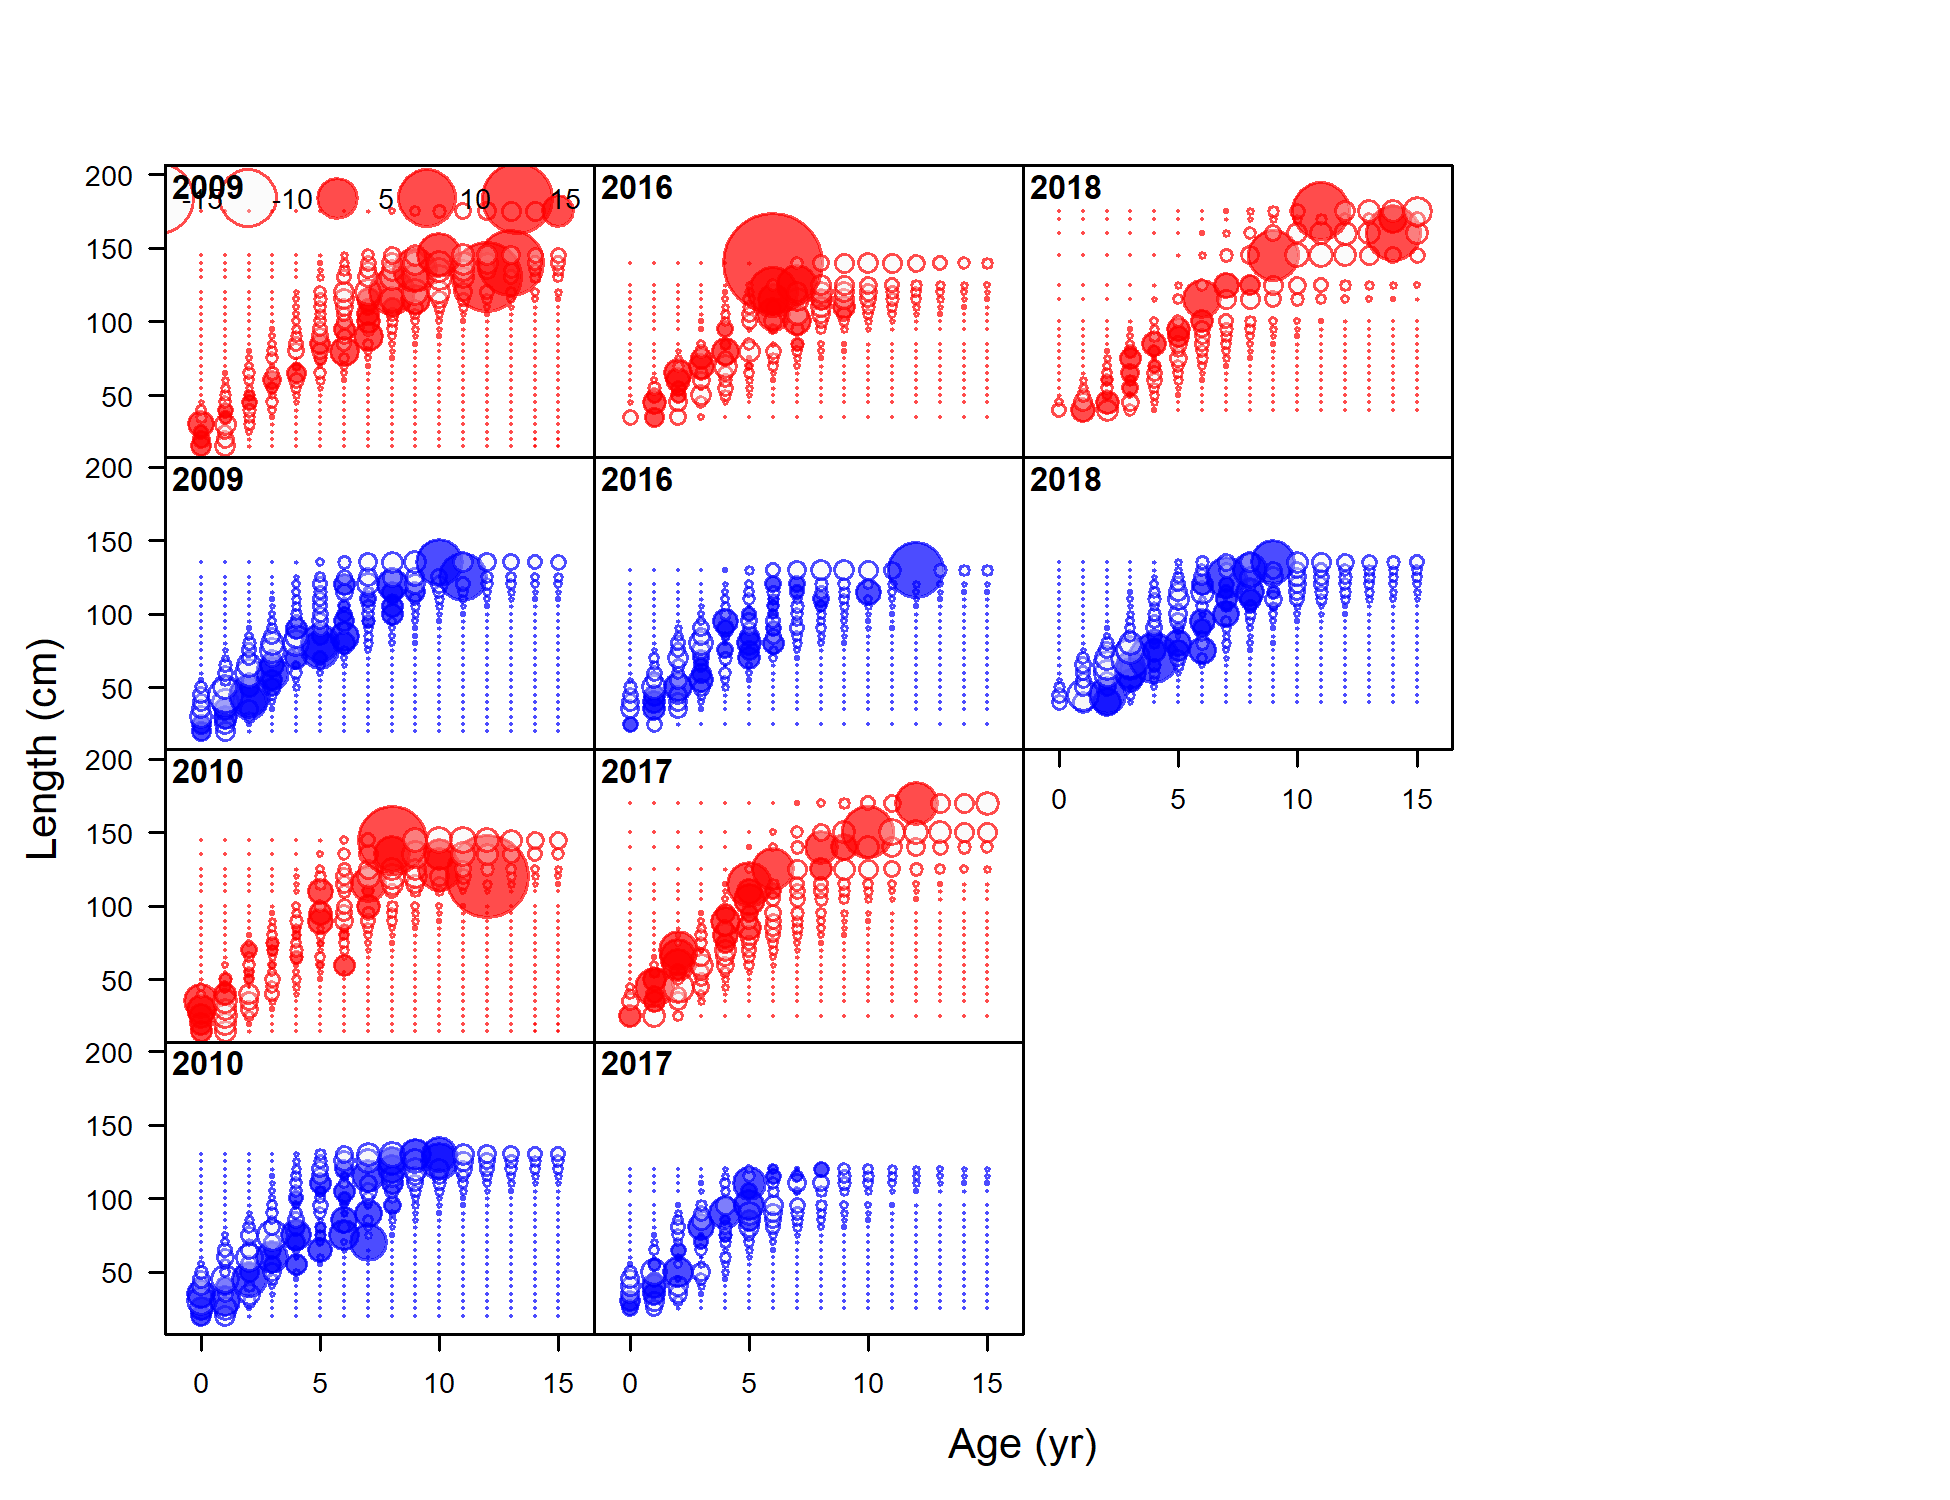
\includegraphics{r4ss/plots_mod1/comp_condAALfit_residsflt5mkt0.png}
\caption{Pearson residuals for the fit to conditional age-at-length data
from the WCGBT Survey. Closed bubbles are positive residuals (observed
\textgreater{} expected) and open bubbles are negative residuals
(observed \textless{} expected). \label{fig:age_fit_WCGBTS}}
\end{figure}

\begin{figure}
\centering
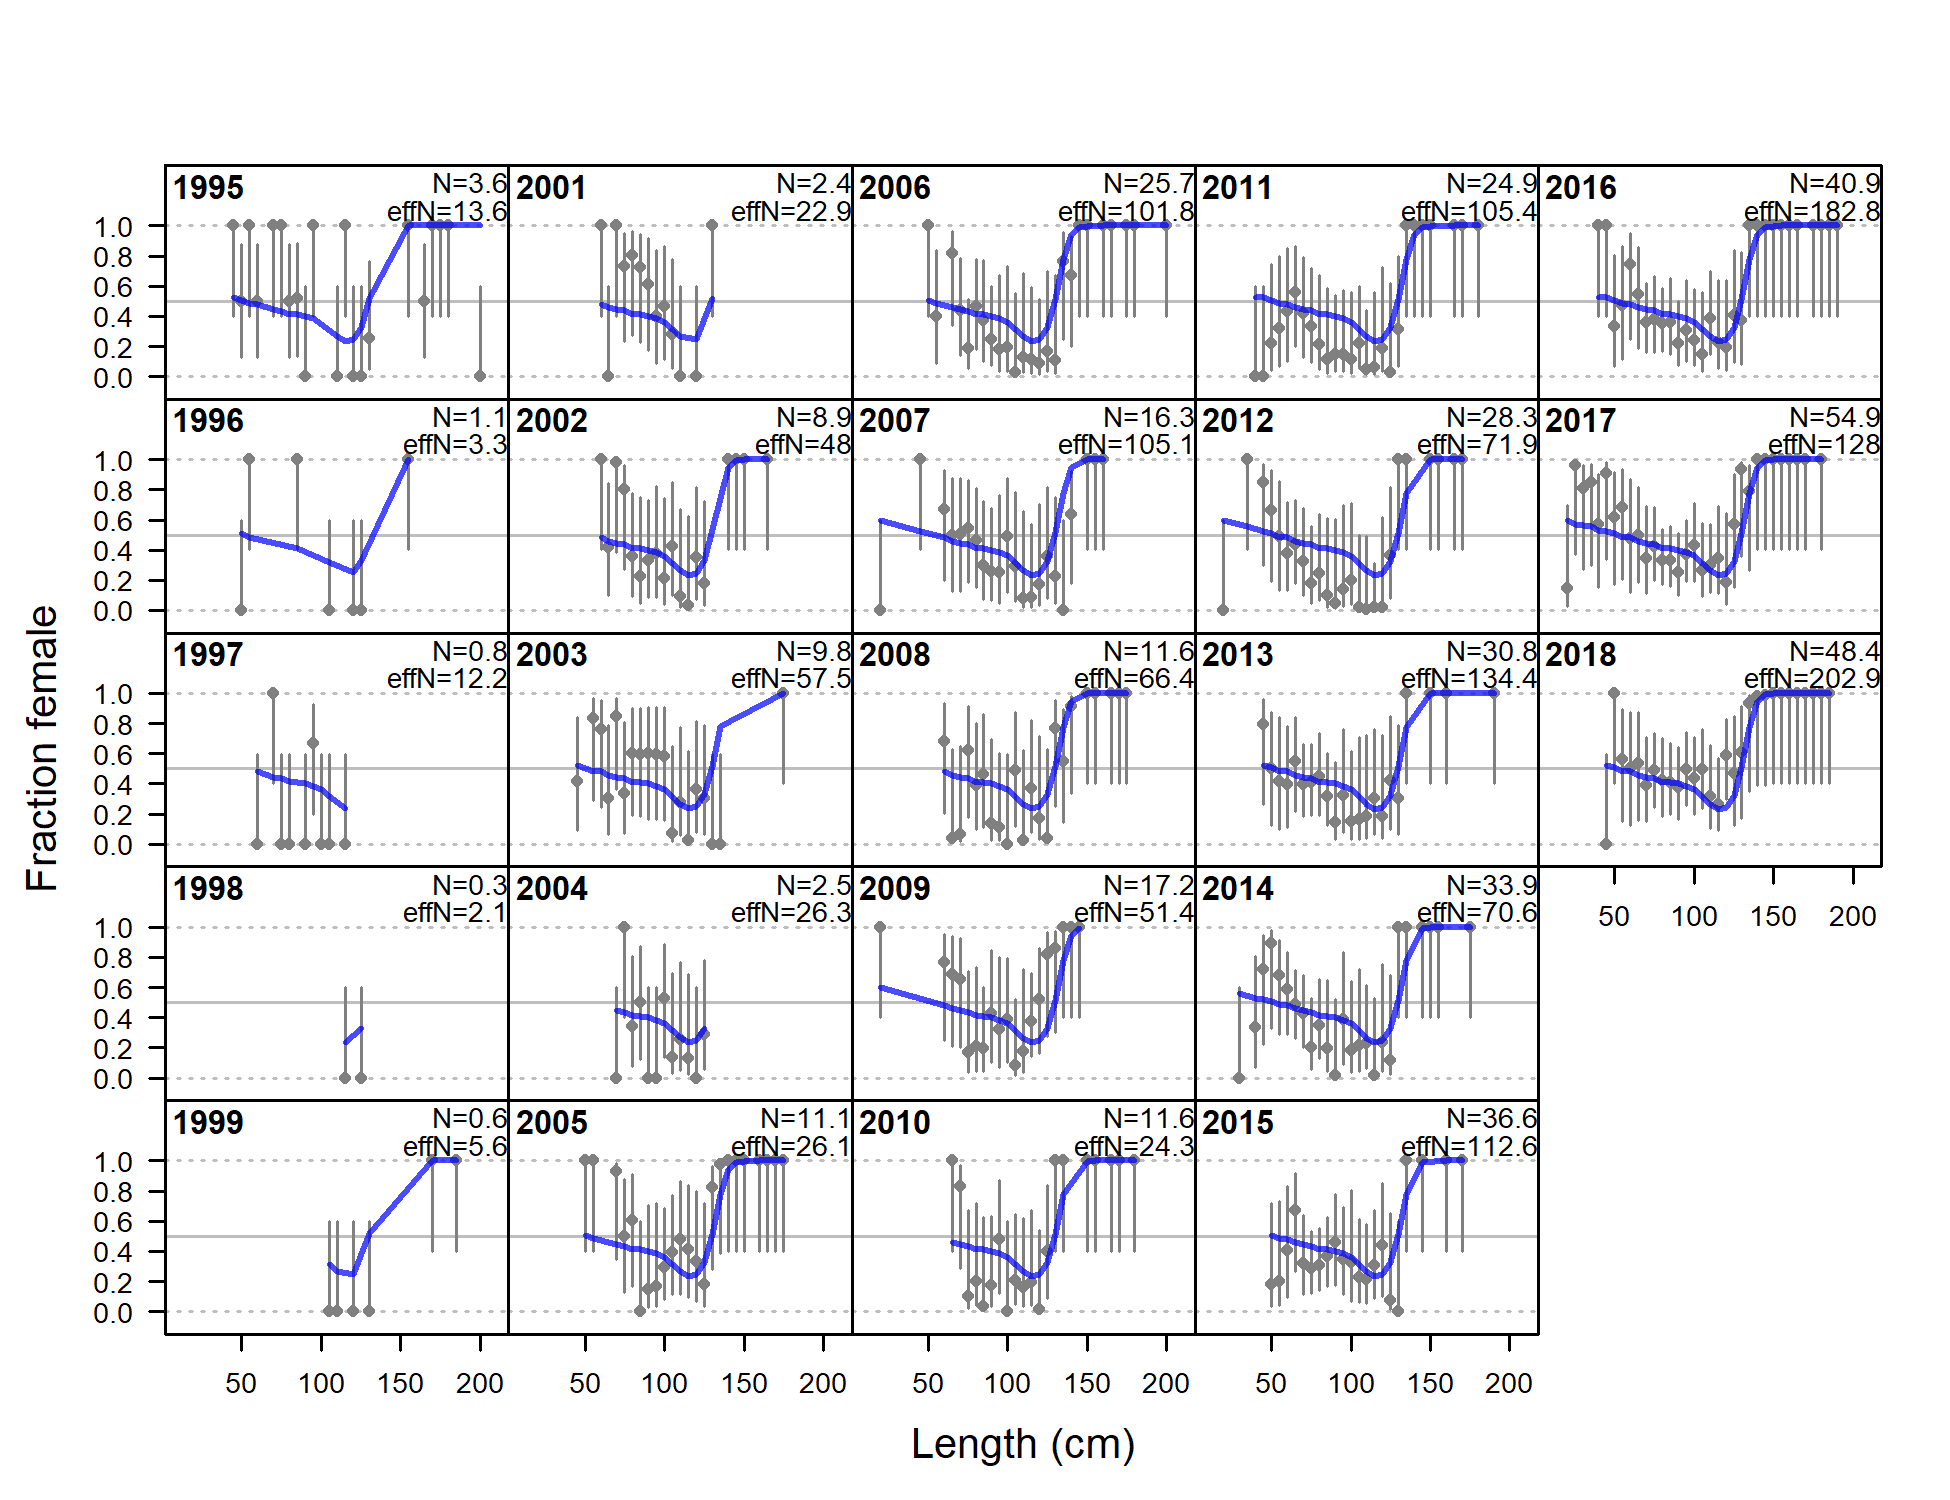
\includegraphics{r4ss/plots_mod1/sexratio_len_flt1mkt2.png}
\caption{Observed sex ratios (points) from the fishery length comp data
with 75\% intervals (vertical lines) calculated as a Jeffreys interval
based on the adjusted input sample size. The model expectation is shown
in the blue line.\label{fig:sexratio_len_flt1mkt2}}
\end{figure}

\begin{figure}
\centering
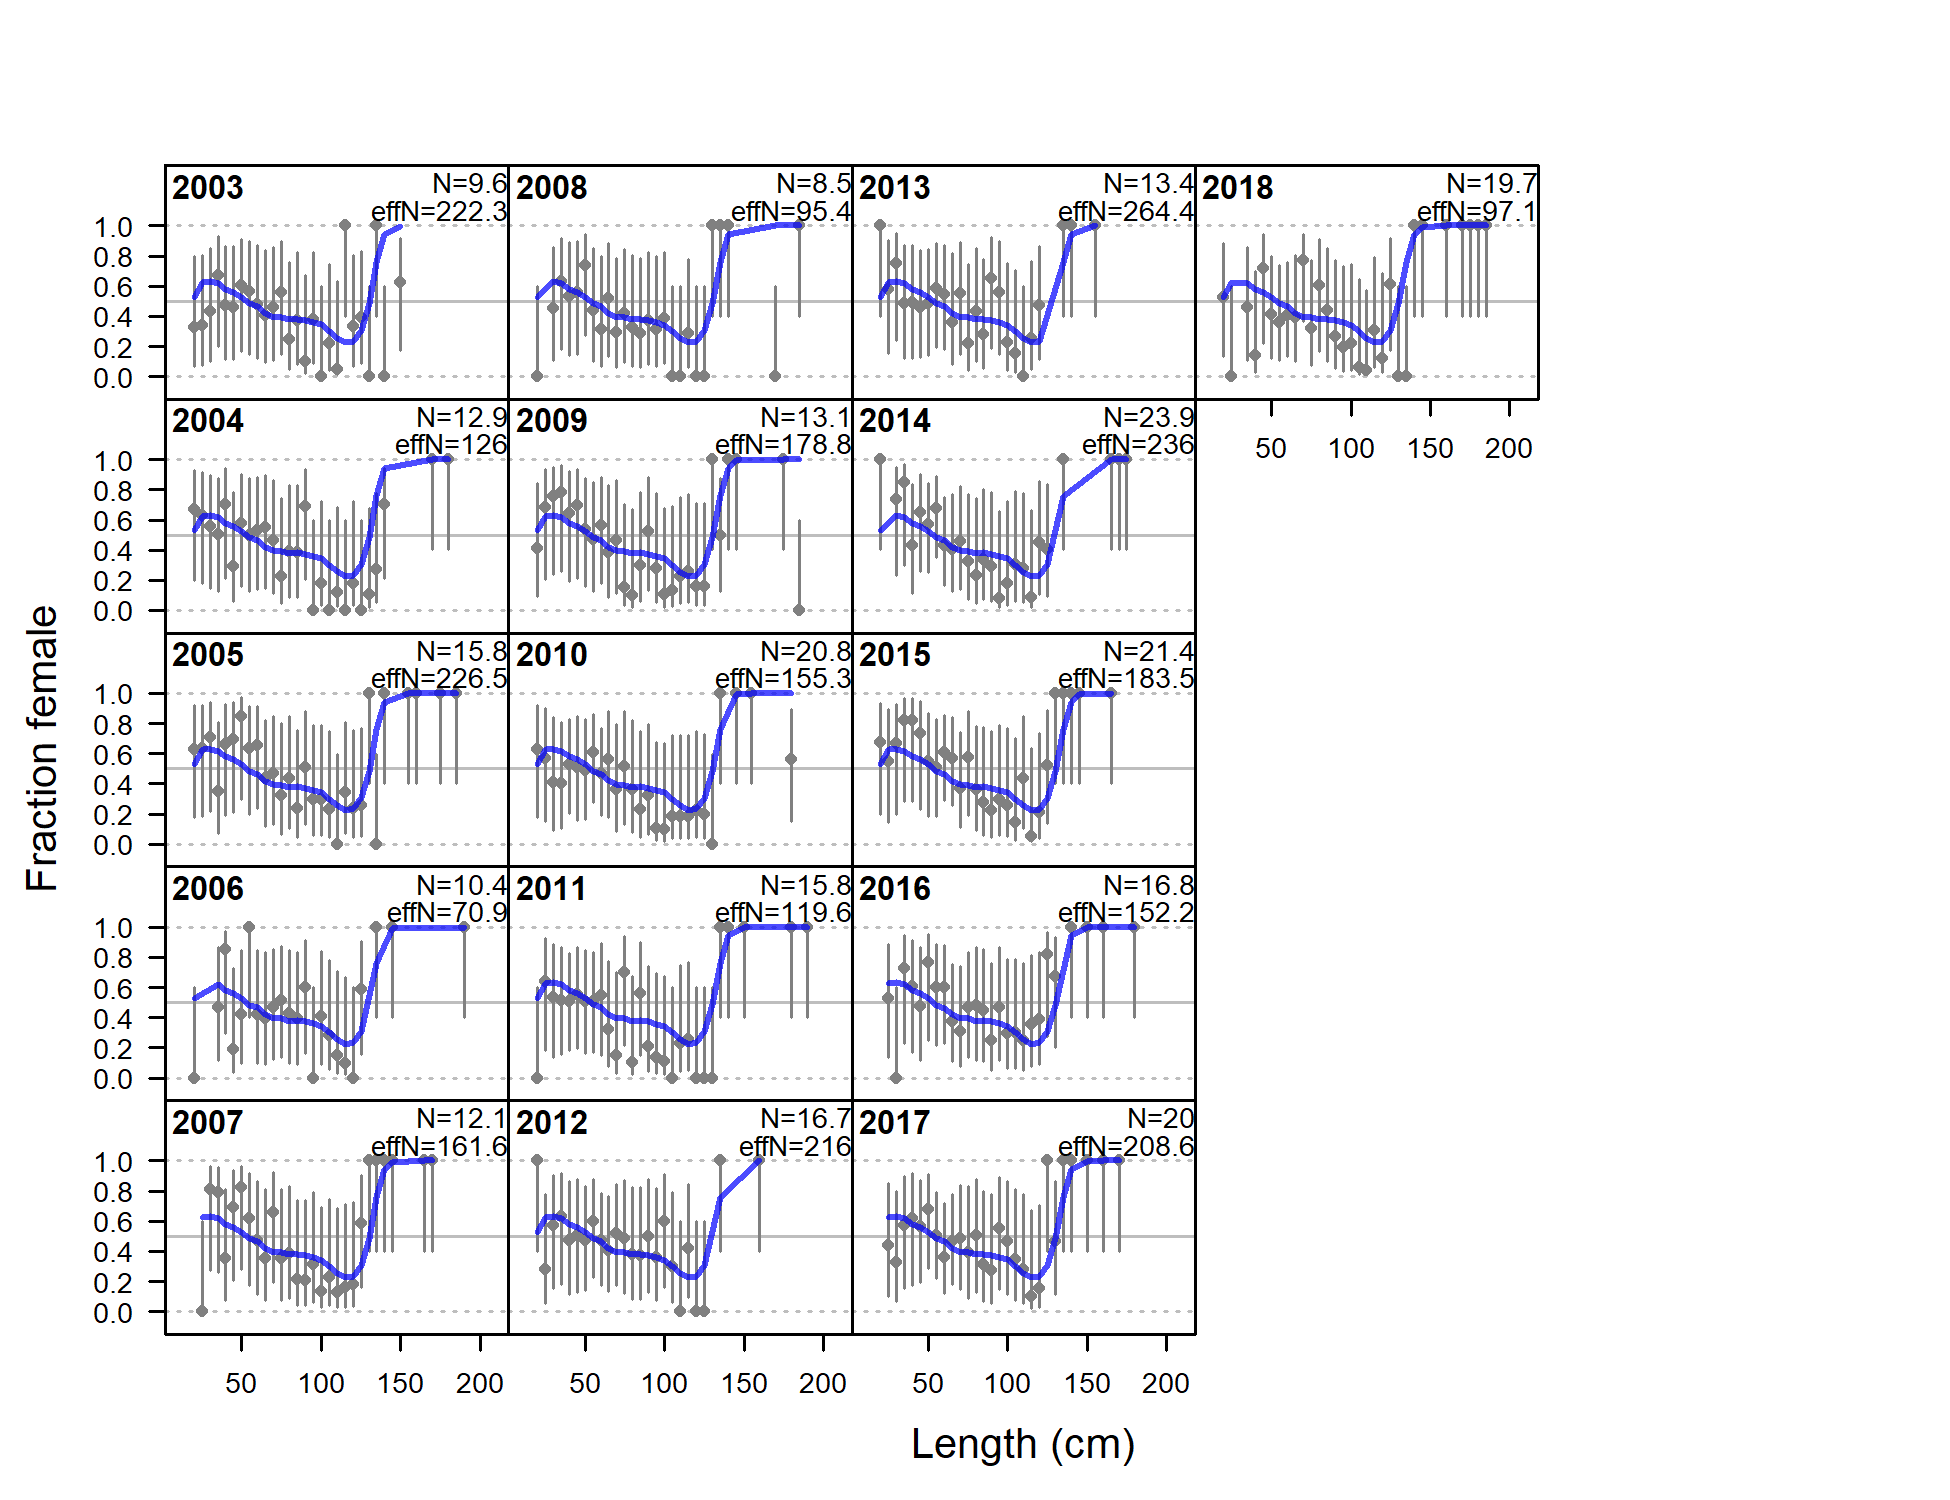
\includegraphics{r4ss/plots_mod1/sexratio_len_flt5mkt0.png}
\caption{Observed sex ratios (points) from the WCGBT Survey length comp
data with 75\% intervals (vertical lines) calculated as a Jeffreys
interval based on the adjusted input sample size. The model expectation
is shown in the blue line.\label{fig:sexratio_len_flt5mkt0}}
\end{figure}

\begin{figure}
\centering
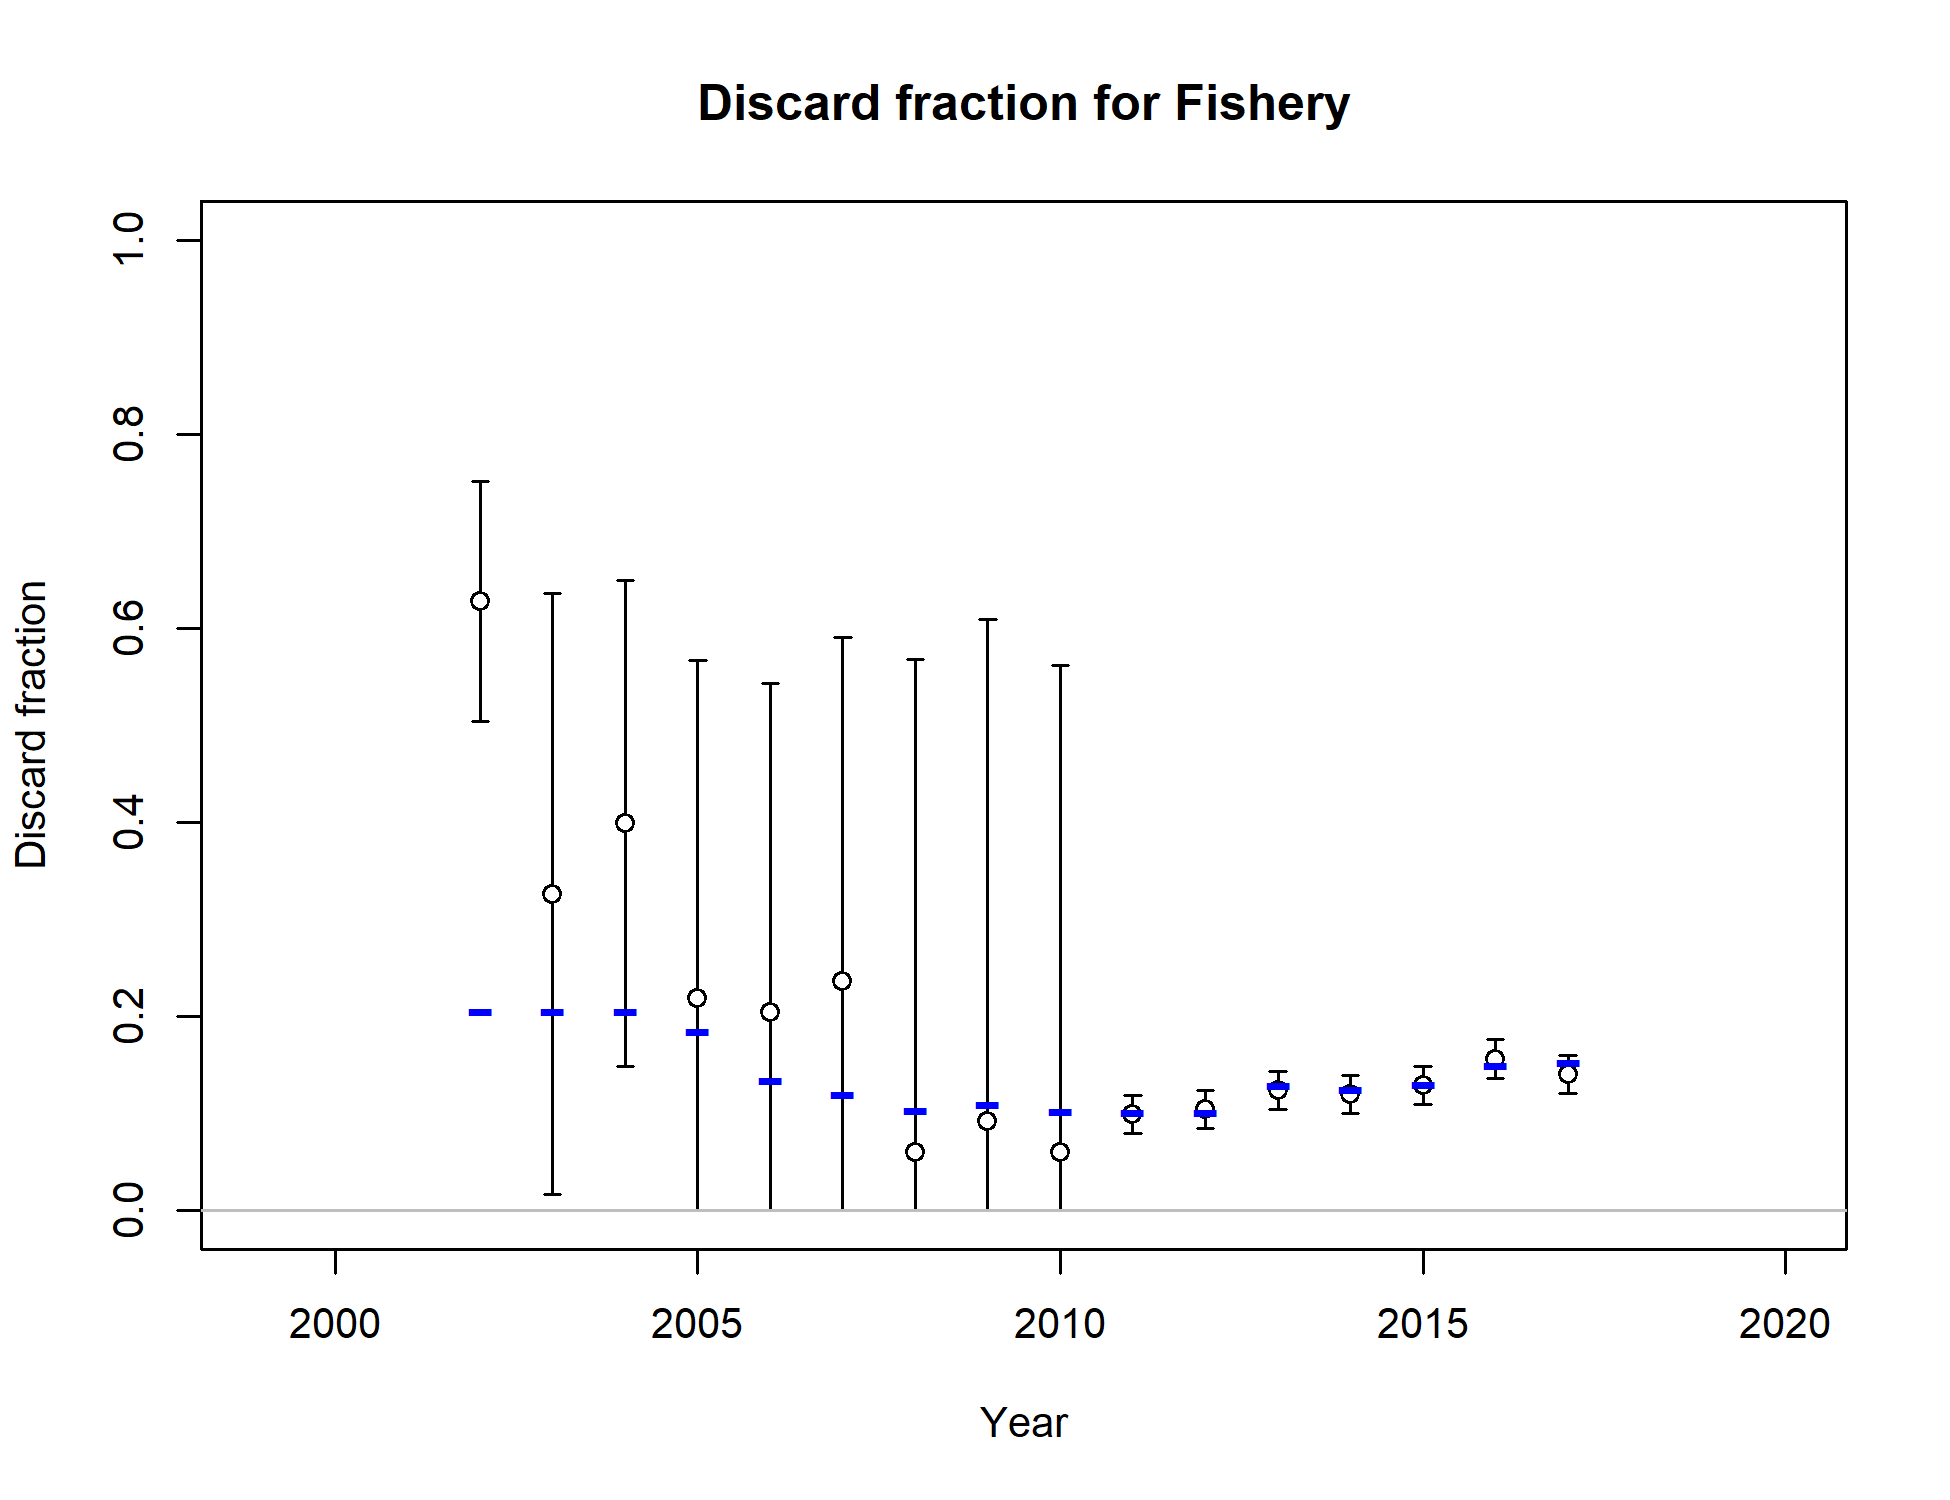
\includegraphics{r4ss/plots_mod1/discard_fitFishery.png}
\caption{Fit to the discard fraction estimates. Points are model
estimates with 95\% uncertainty intervals. The model estimate is shown
in the blue lines.\label{fig:discard_fitFishery}}
\end{figure}

\begin{figure}
\centering
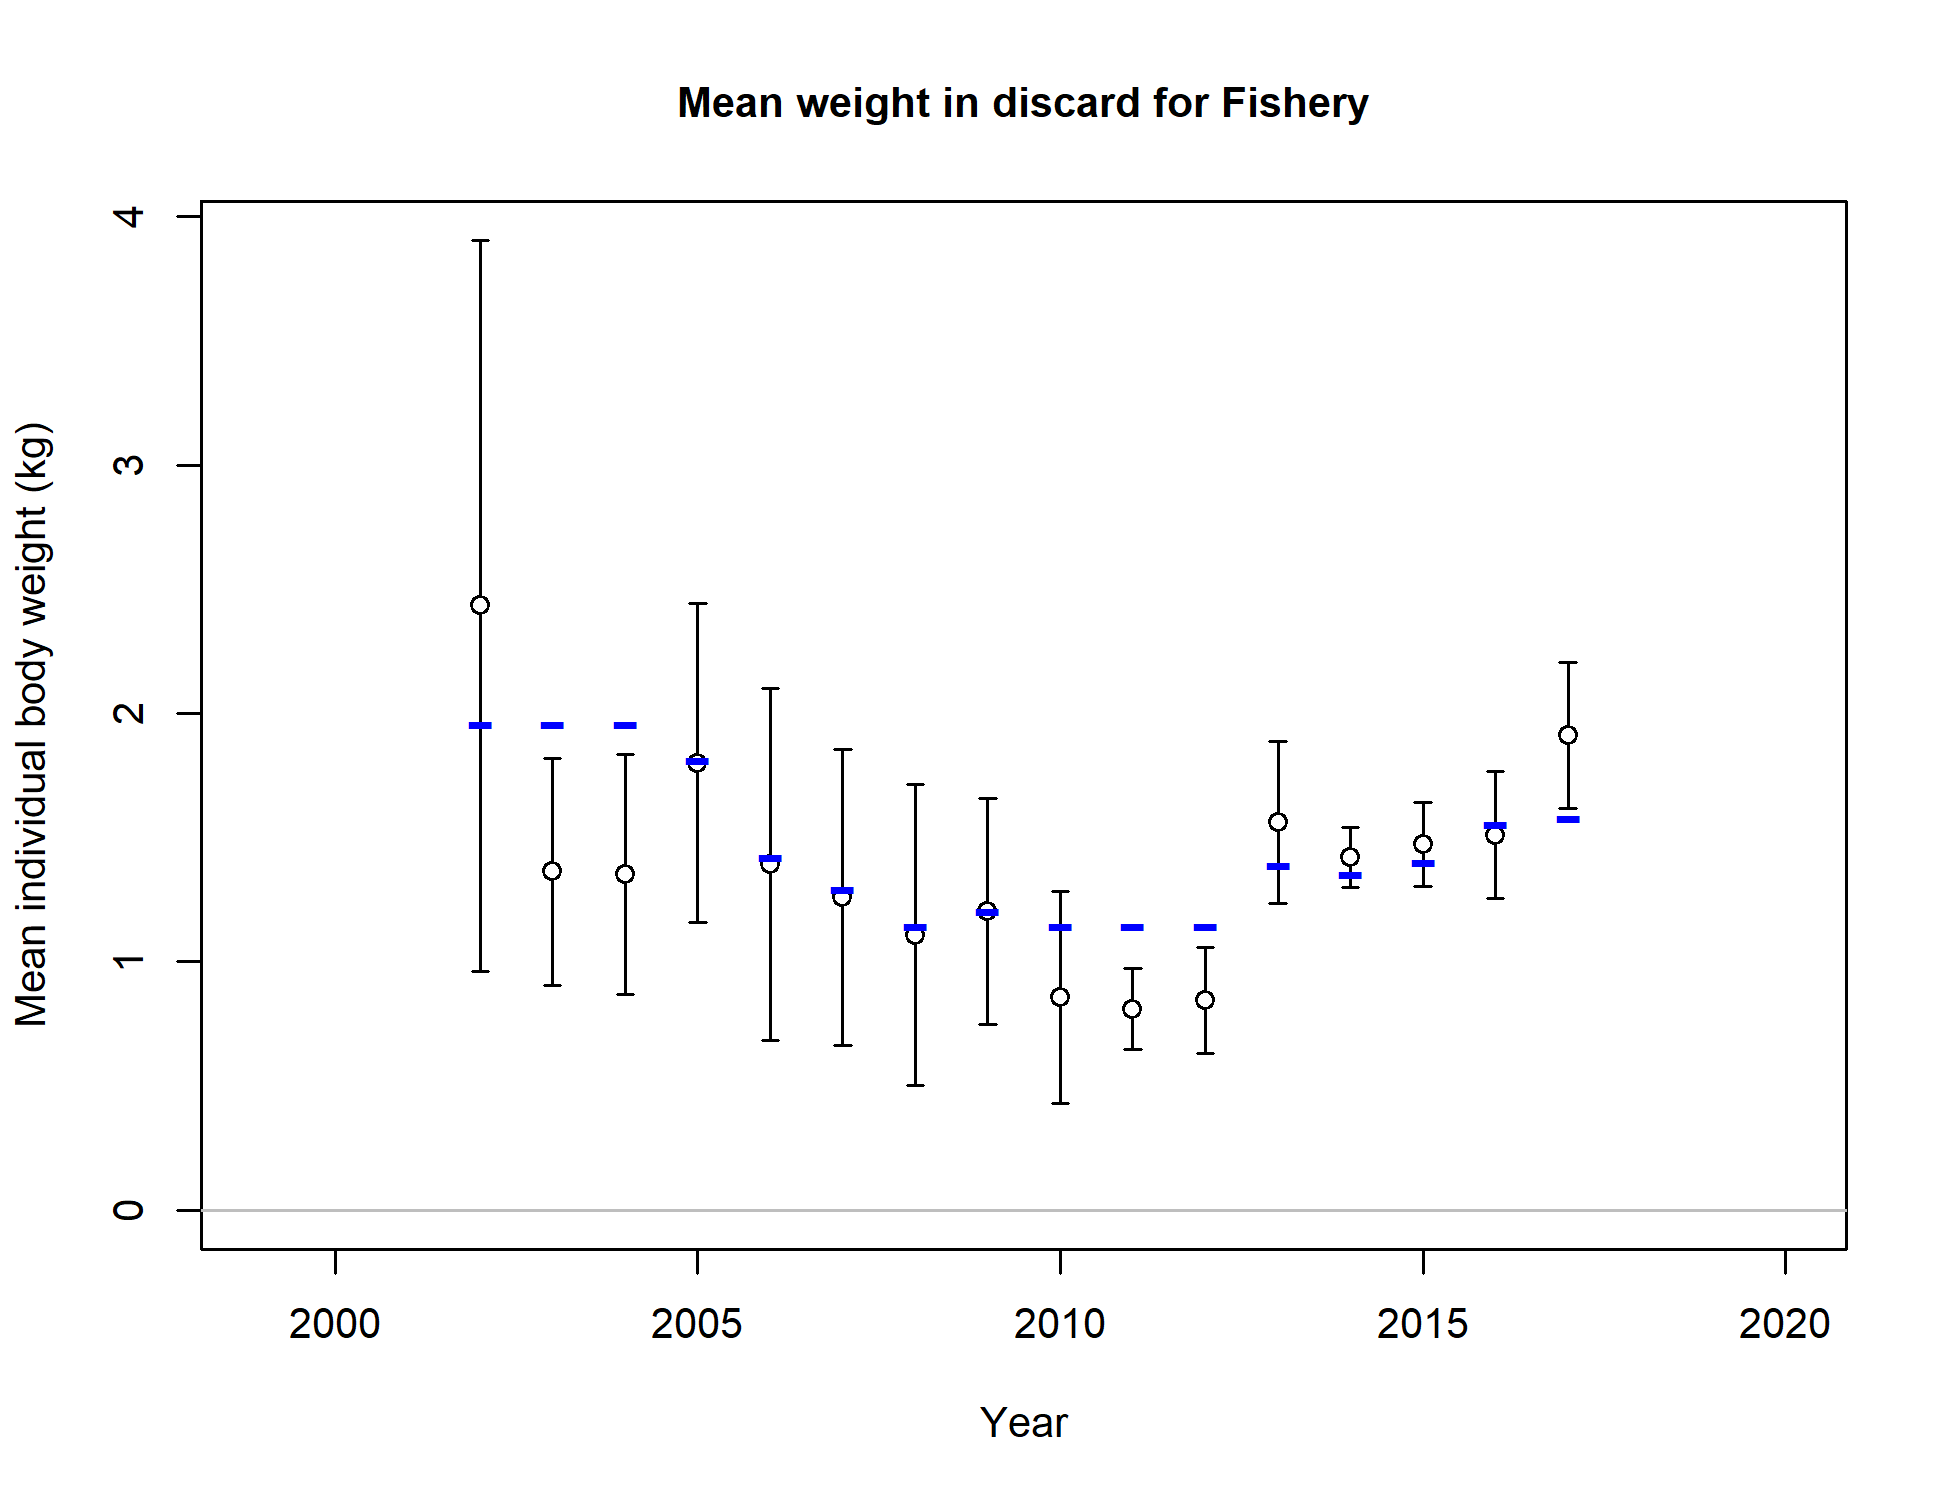
\includegraphics{r4ss/plots_mod1/bodywt_fit_fltFishery.png}
\caption{Fit to the mean weight of the discards. Points are model
estimates with 95\% uncertainty intervals. The model estimate is shown
in the blue lines.\label{fig:bodywt_fit_fltFishery}}
\end{figure}

\FloatBarrier

\newpage

\hypertarget{time-series-figures}{%
\subsubsection{Time Series Figures}\label{time-series-figures}}

\FloatBarrier

\vspace{.5cm}

\begin{figure}
\centering
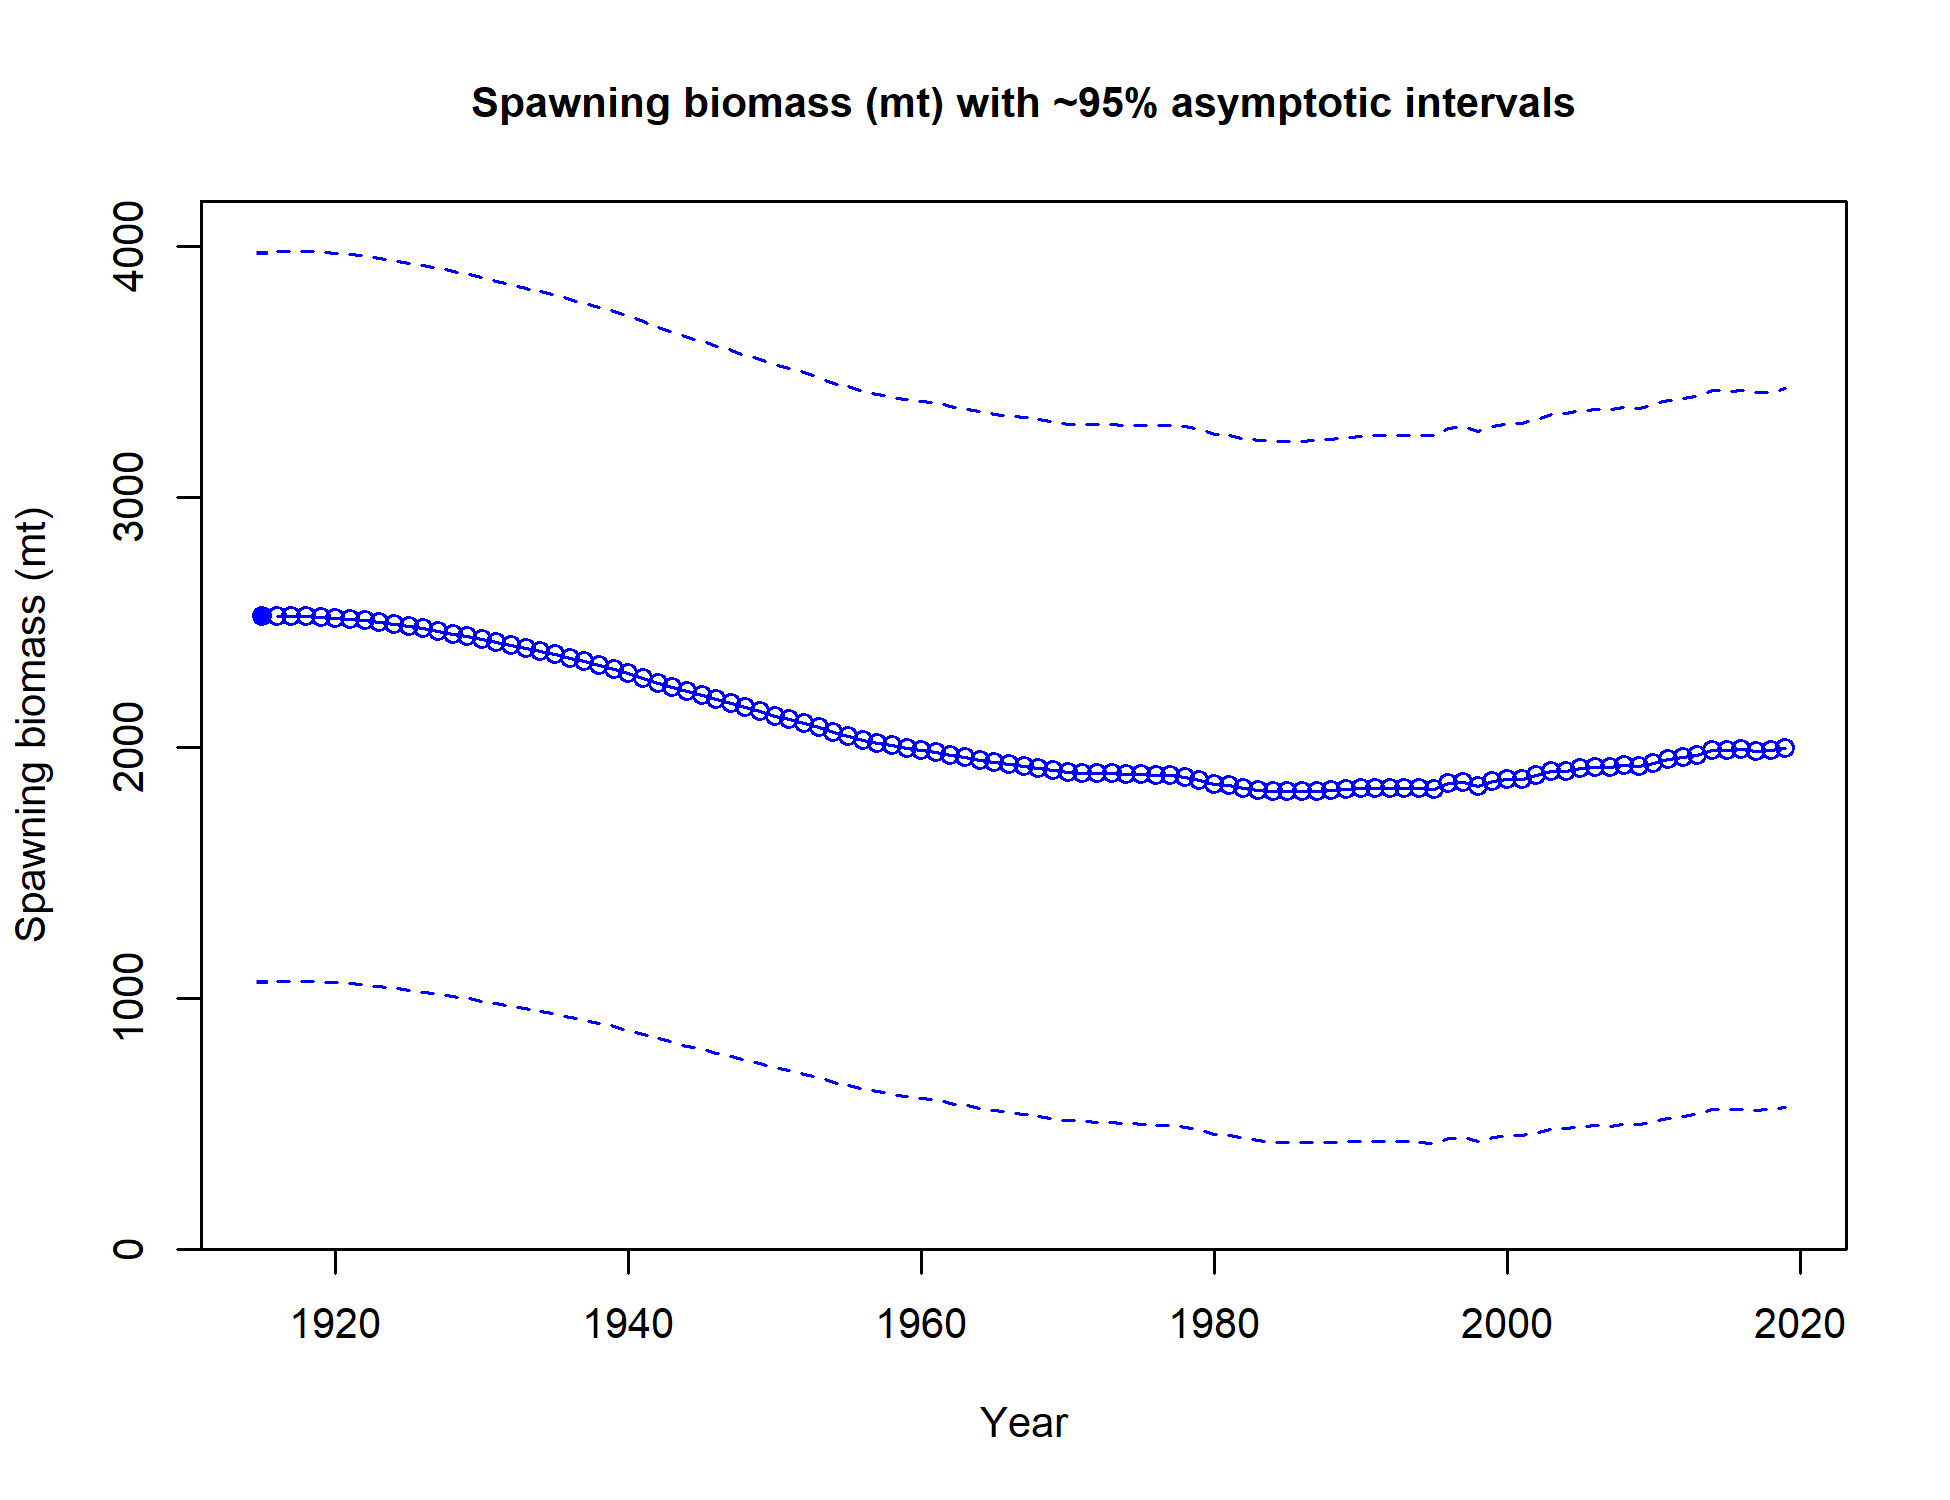
\includegraphics{r4ss/plots_mod1/ts7_Spawning_biomass_(mt)_with_95_asymptotic_intervals_intervals.png}
\caption{Estimated spawning biomass (mt) with approximate 95\%
asymptotic intervals.
\label{fig:ts7_Spawning_biomass_(mt)_with_95_asymptotic_intervals_intervals}}
\end{figure}

\begin{figure}
\centering
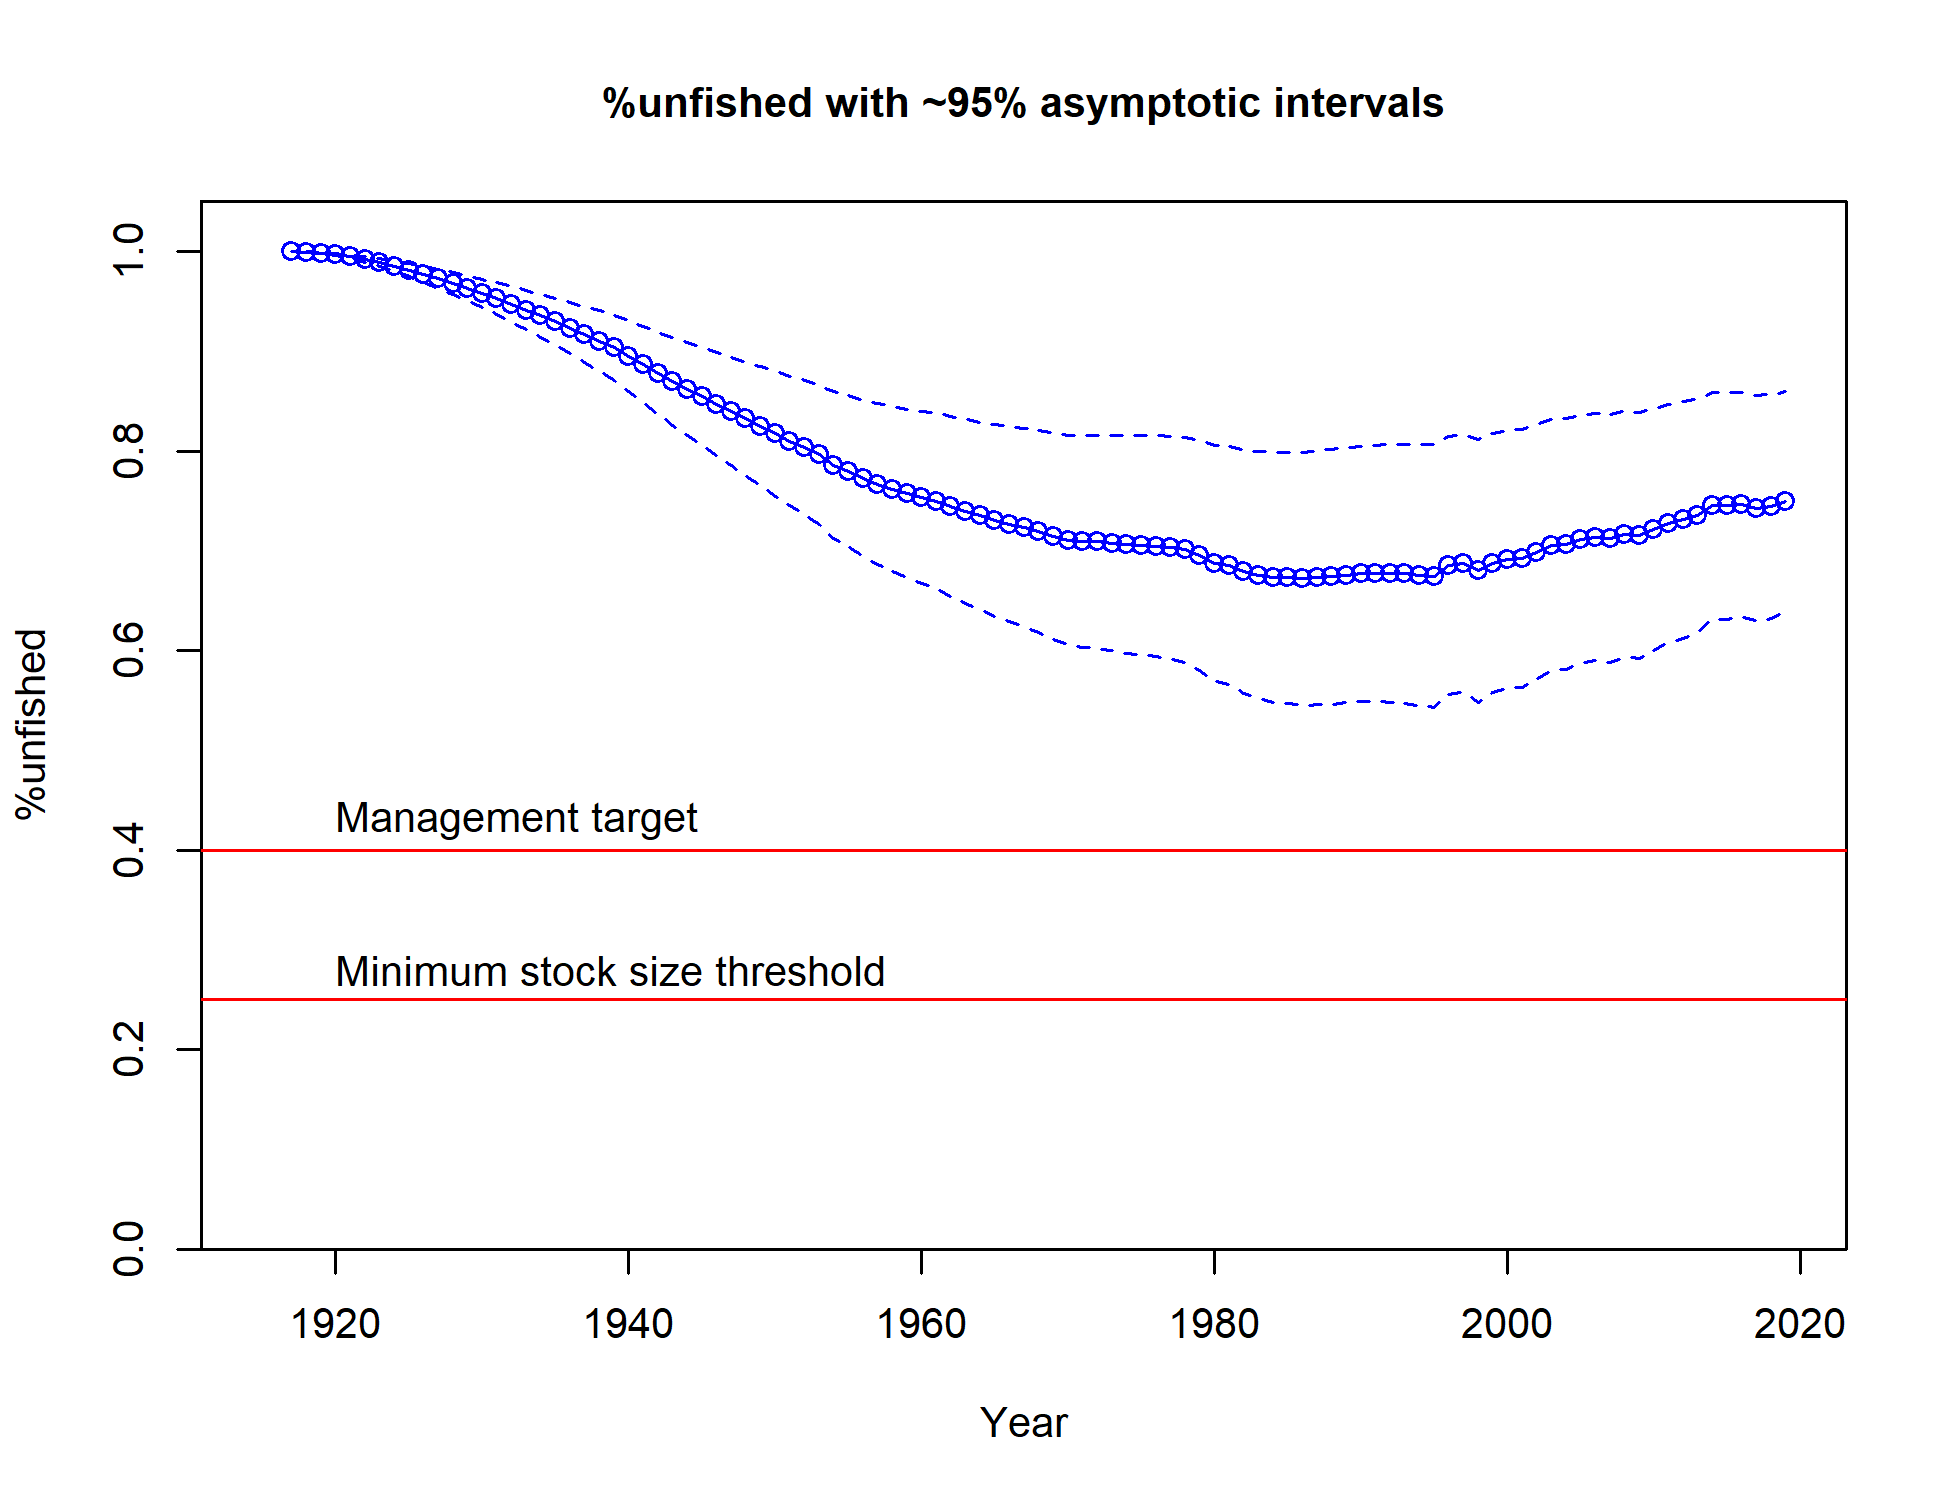
\includegraphics{r4ss/plots_mod1/ts9_unfished_with_95_asymptotic_intervals_intervals.png}
\caption{Estimated \%unfished with approximate 95\% asymptotic
intervals.
\label{fig:ts9_unfished_with_95_asymptotic_intervals_intervals}}
\end{figure}

\begin{figure}
\centering
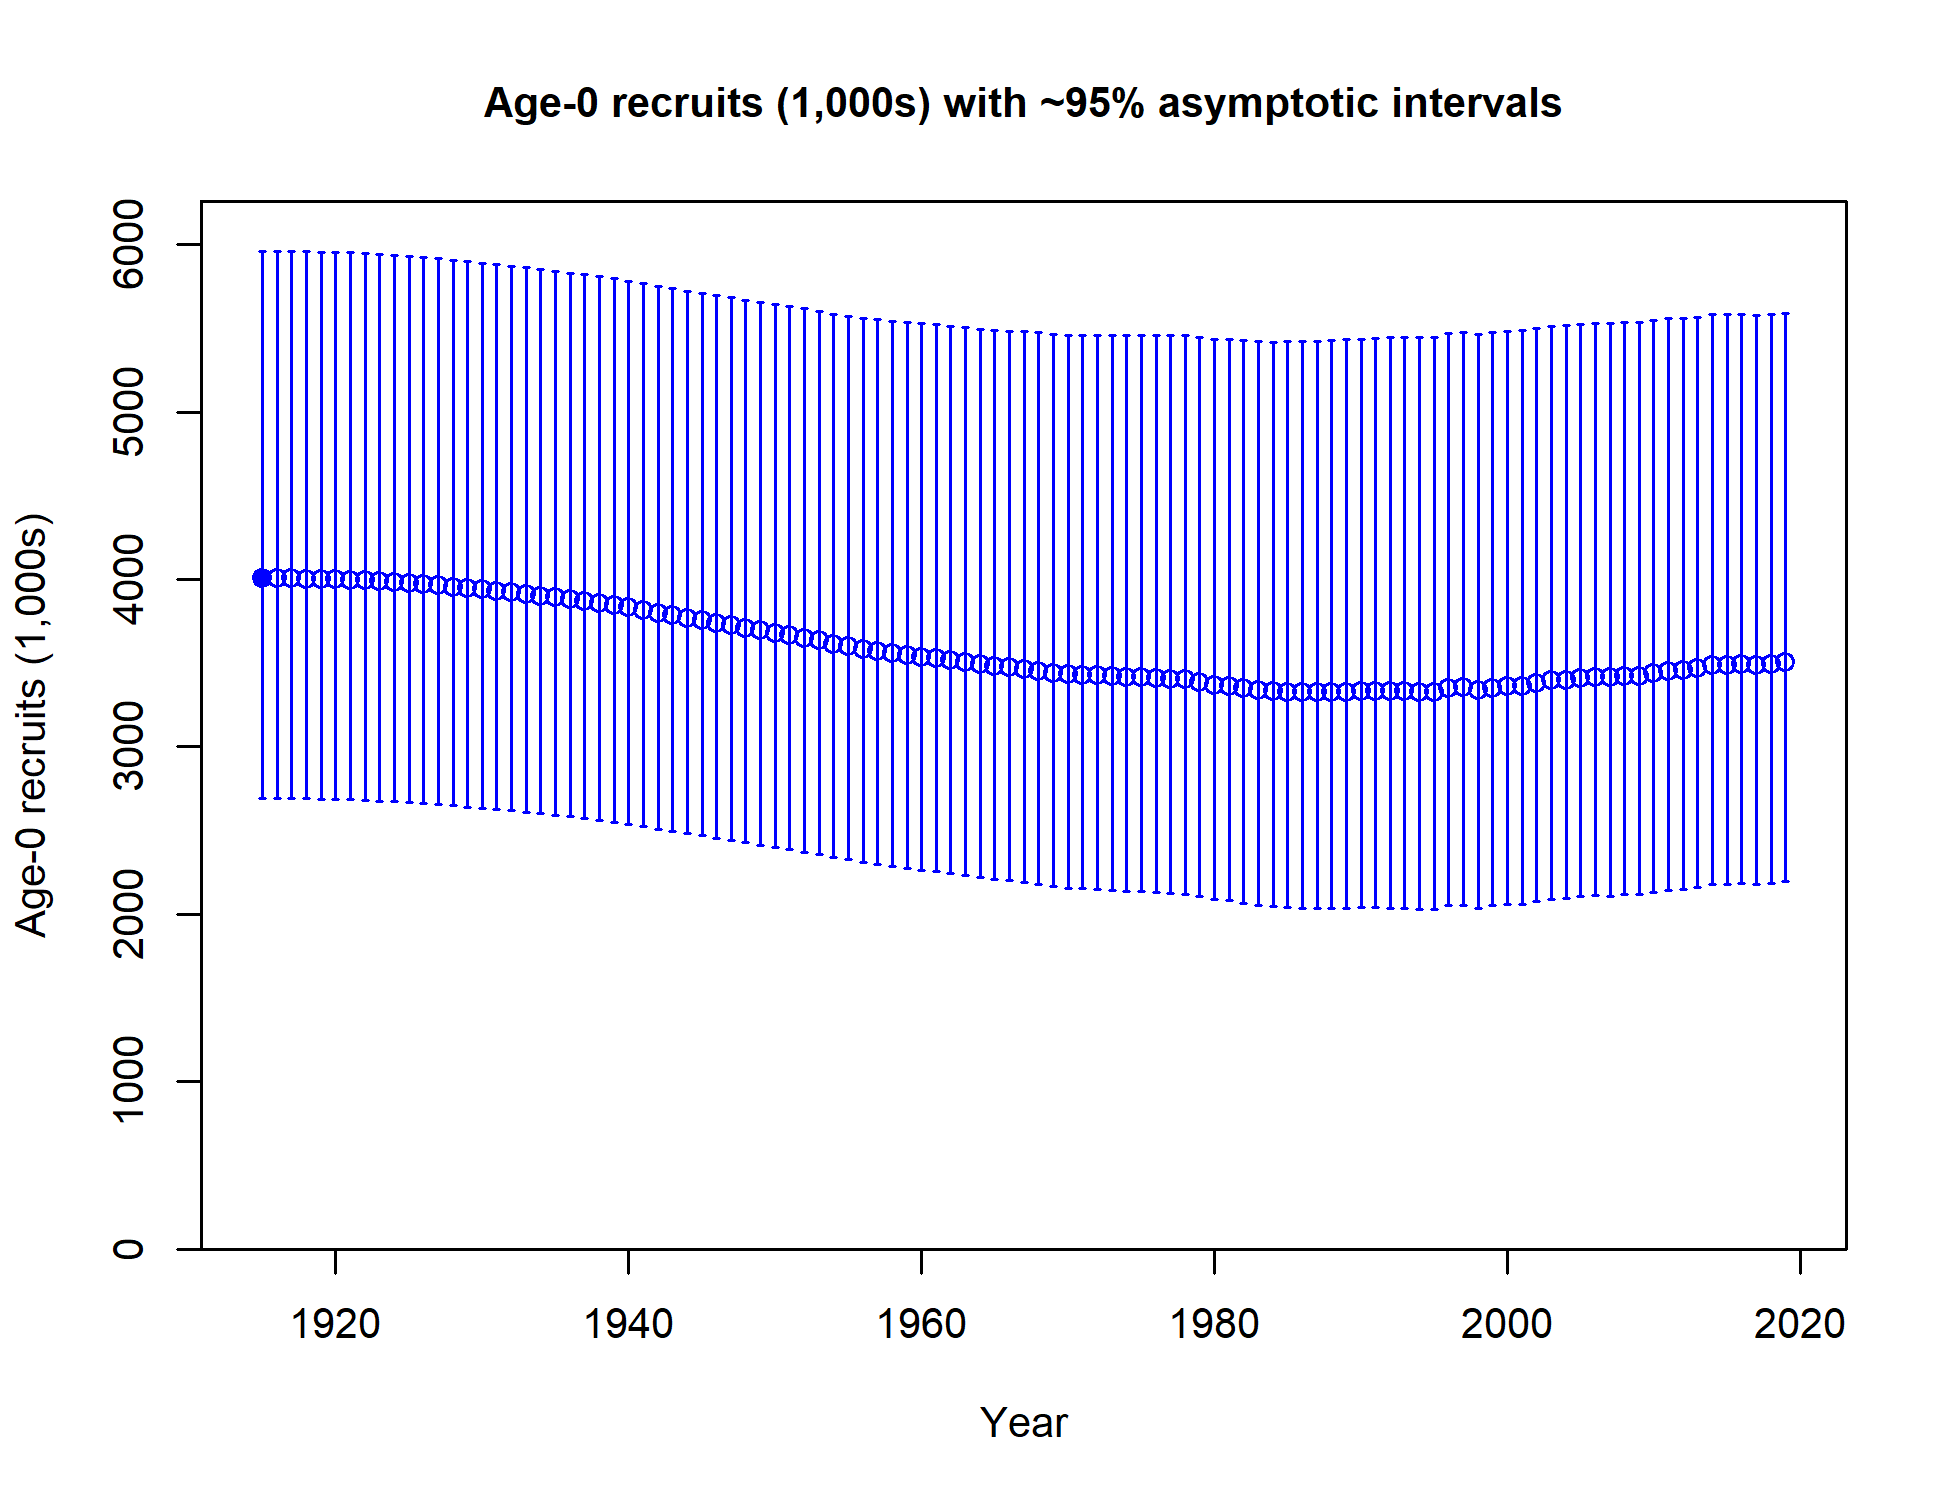
\includegraphics{r4ss/plots_mod1/ts11_Age-0_recruits_(1000s)_with_95_asymptotic_intervals.png}
\caption{Estimated time-series of recruitment for Big Skate.
\label{fig:ts11_Age-0_recruits_(1000s)_with_95_asymptotic_intervals}}
\end{figure}

\begin{figure}
\centering
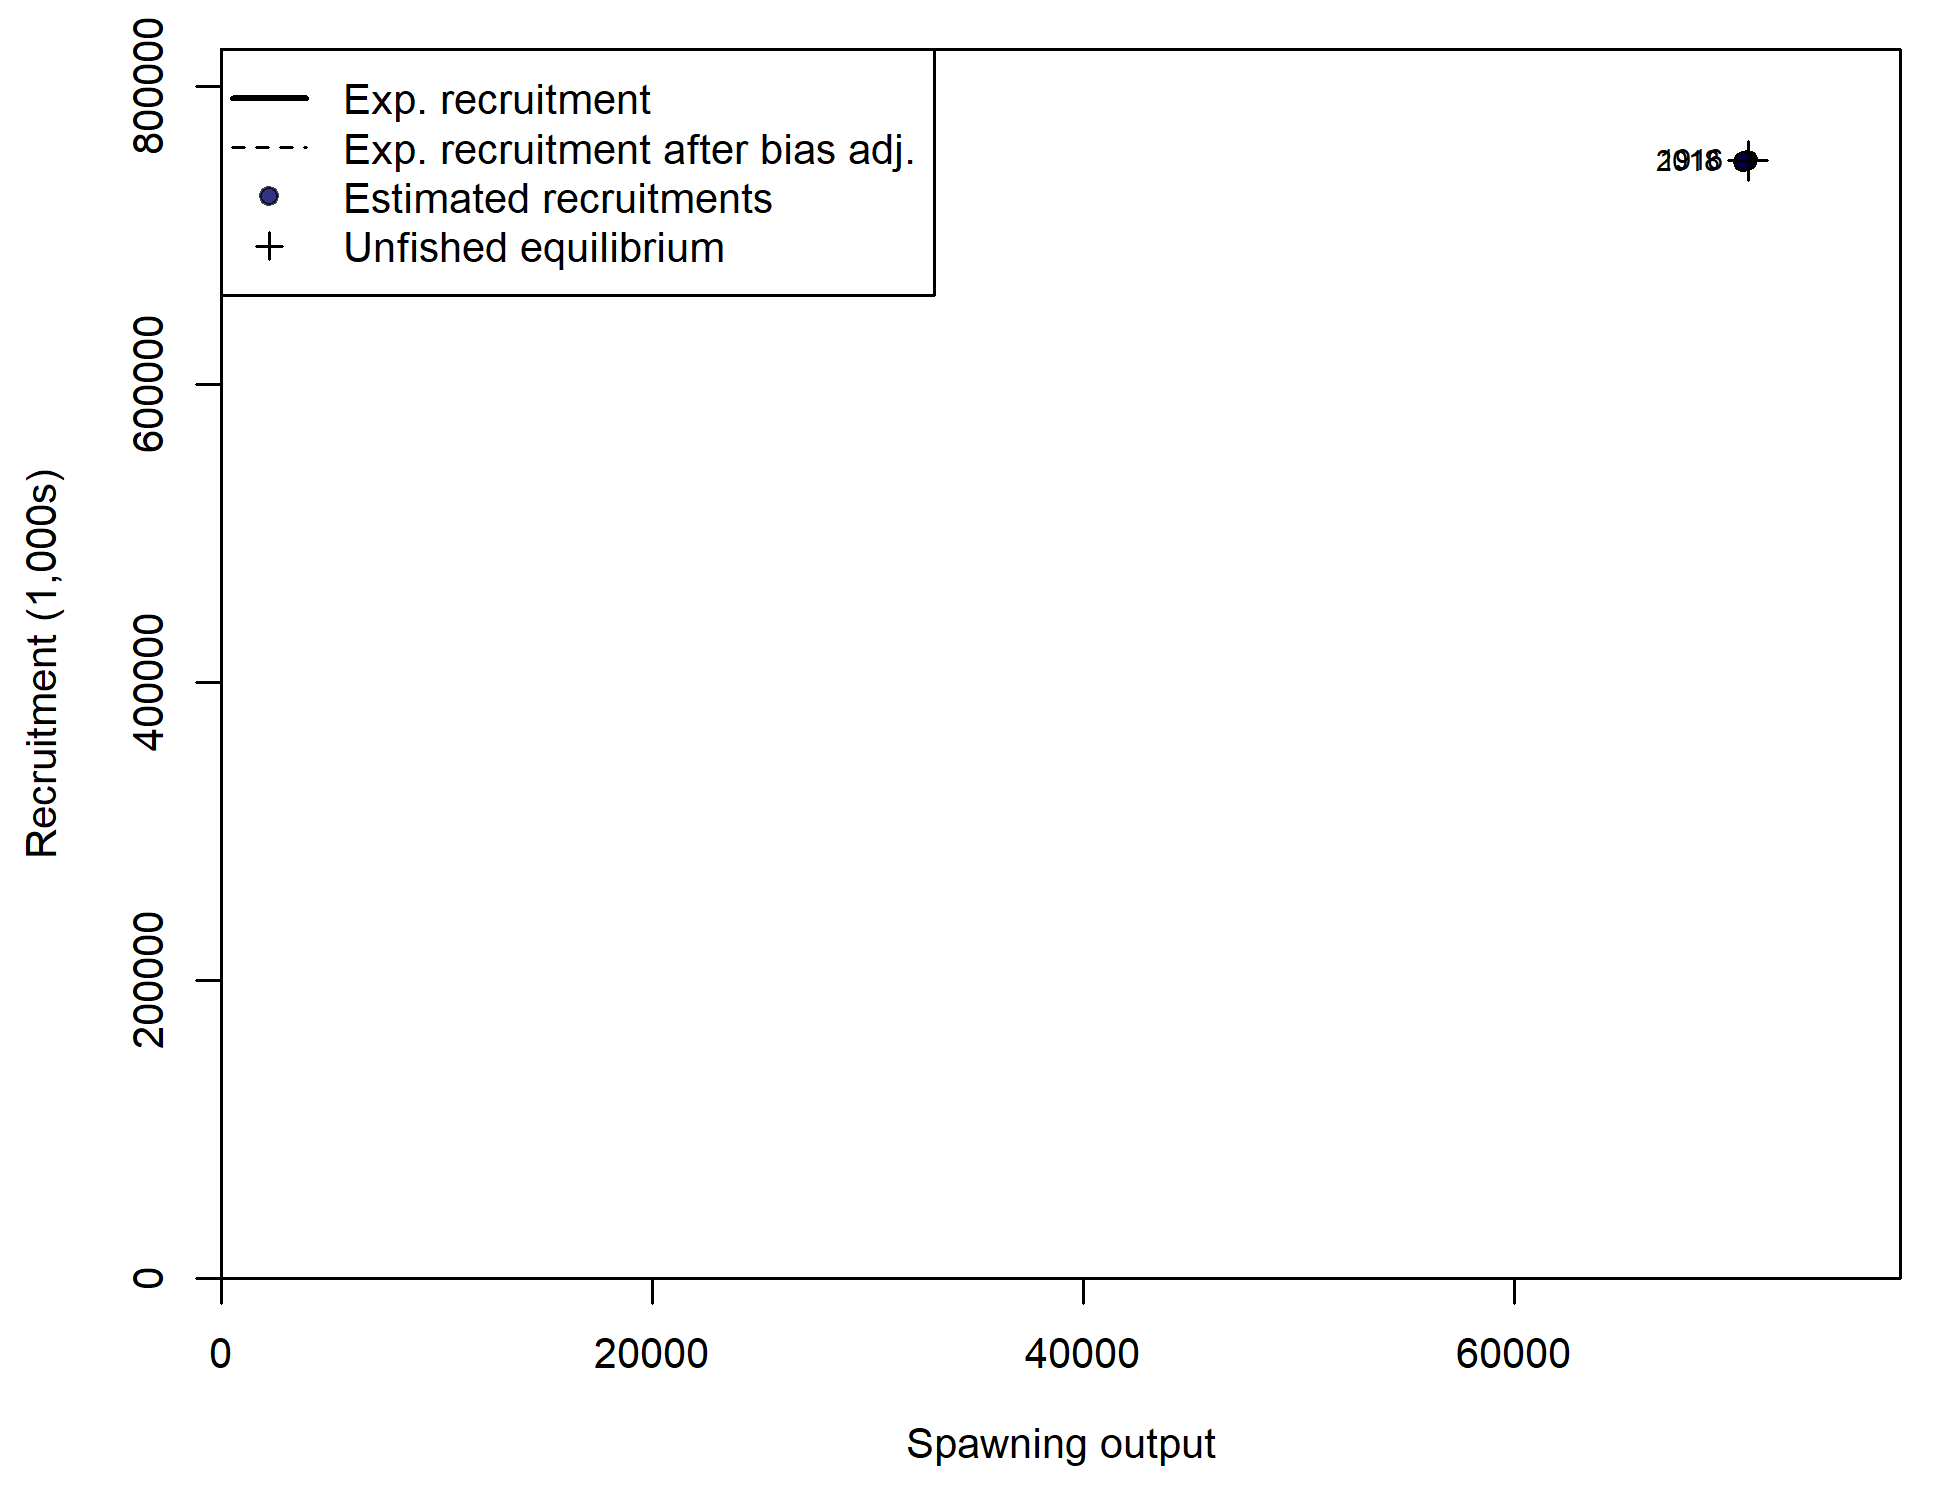
\includegraphics{r4ss/plots_mod1/SR_curve2.png}
\caption{Estimated recruitment and the assumed stock-recruit
relationship. \label{fig:SR_curve2}}
\end{figure}

\begin{figure}
\centering
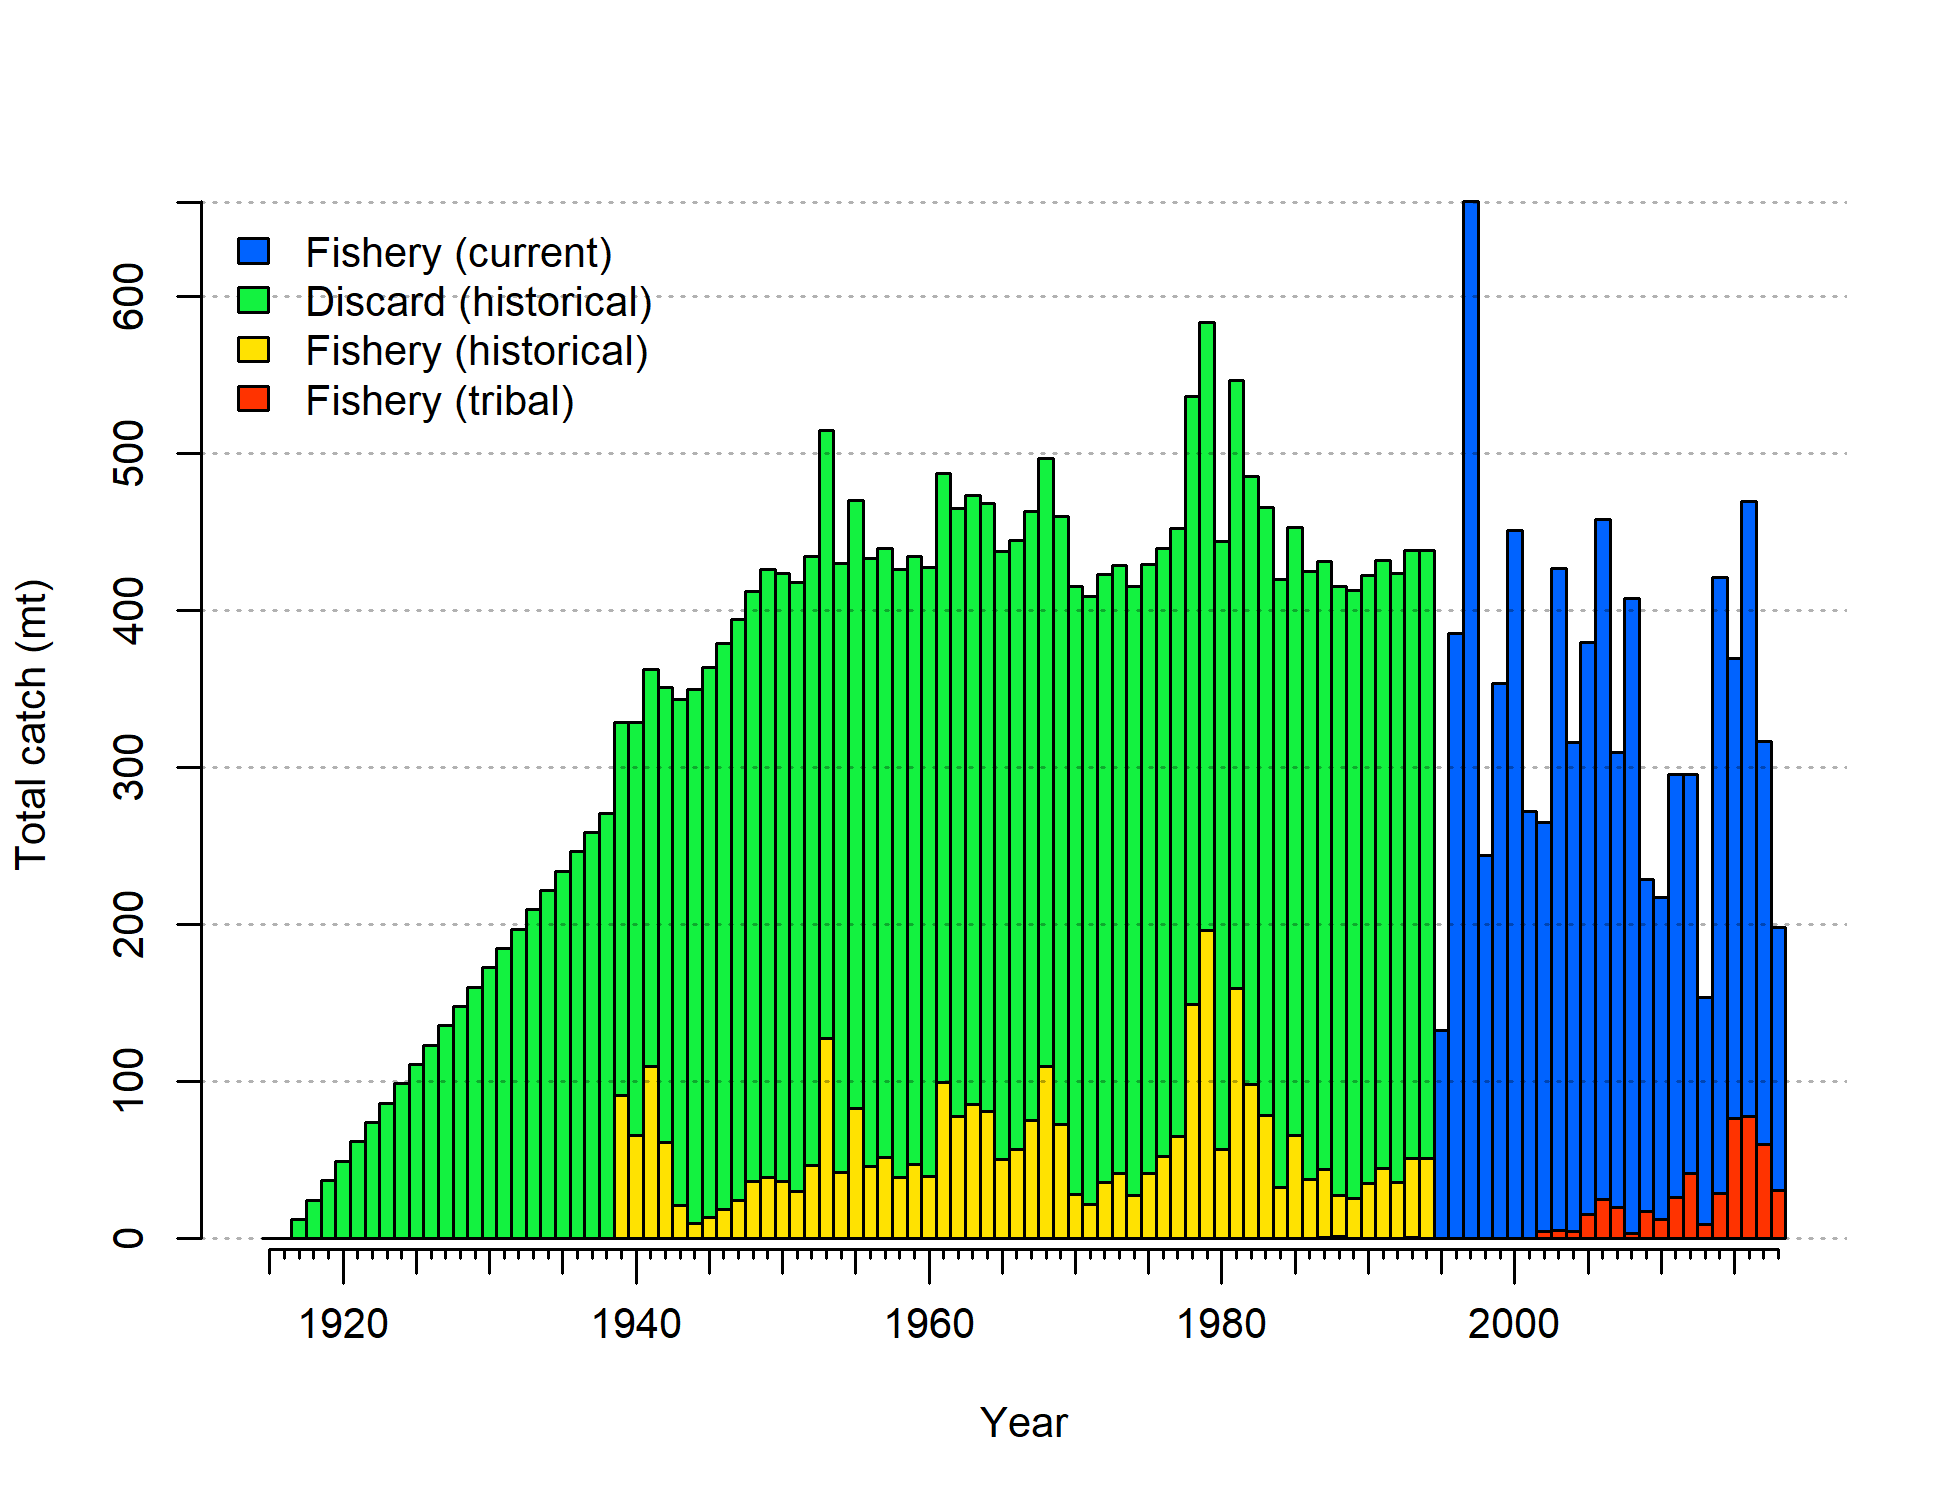
\includegraphics{r4ss/plots_mod1/catch5 total catch (including discards) stacked.png}
\caption{Estimated total catch including discards estimated within the
model. The historical discards shown in green have been scaled to
account for an assumed 50\% discard mortality but the discards in the
recent period show both live and dead discards.
\label{fig:catch_total_plot}}
\end{figure}

\FloatBarrier

\newpage

\hypertarget{sensitivity-analyses-and-retrospectives}{%
\subsubsection{Sensitivity Analyses and
Retrospectives}\label{sensitivity-analyses-and-retrospectives}}

\FloatBarrier

\vspace{.5cm}

\begin{figure}[h]
\begin{centering}
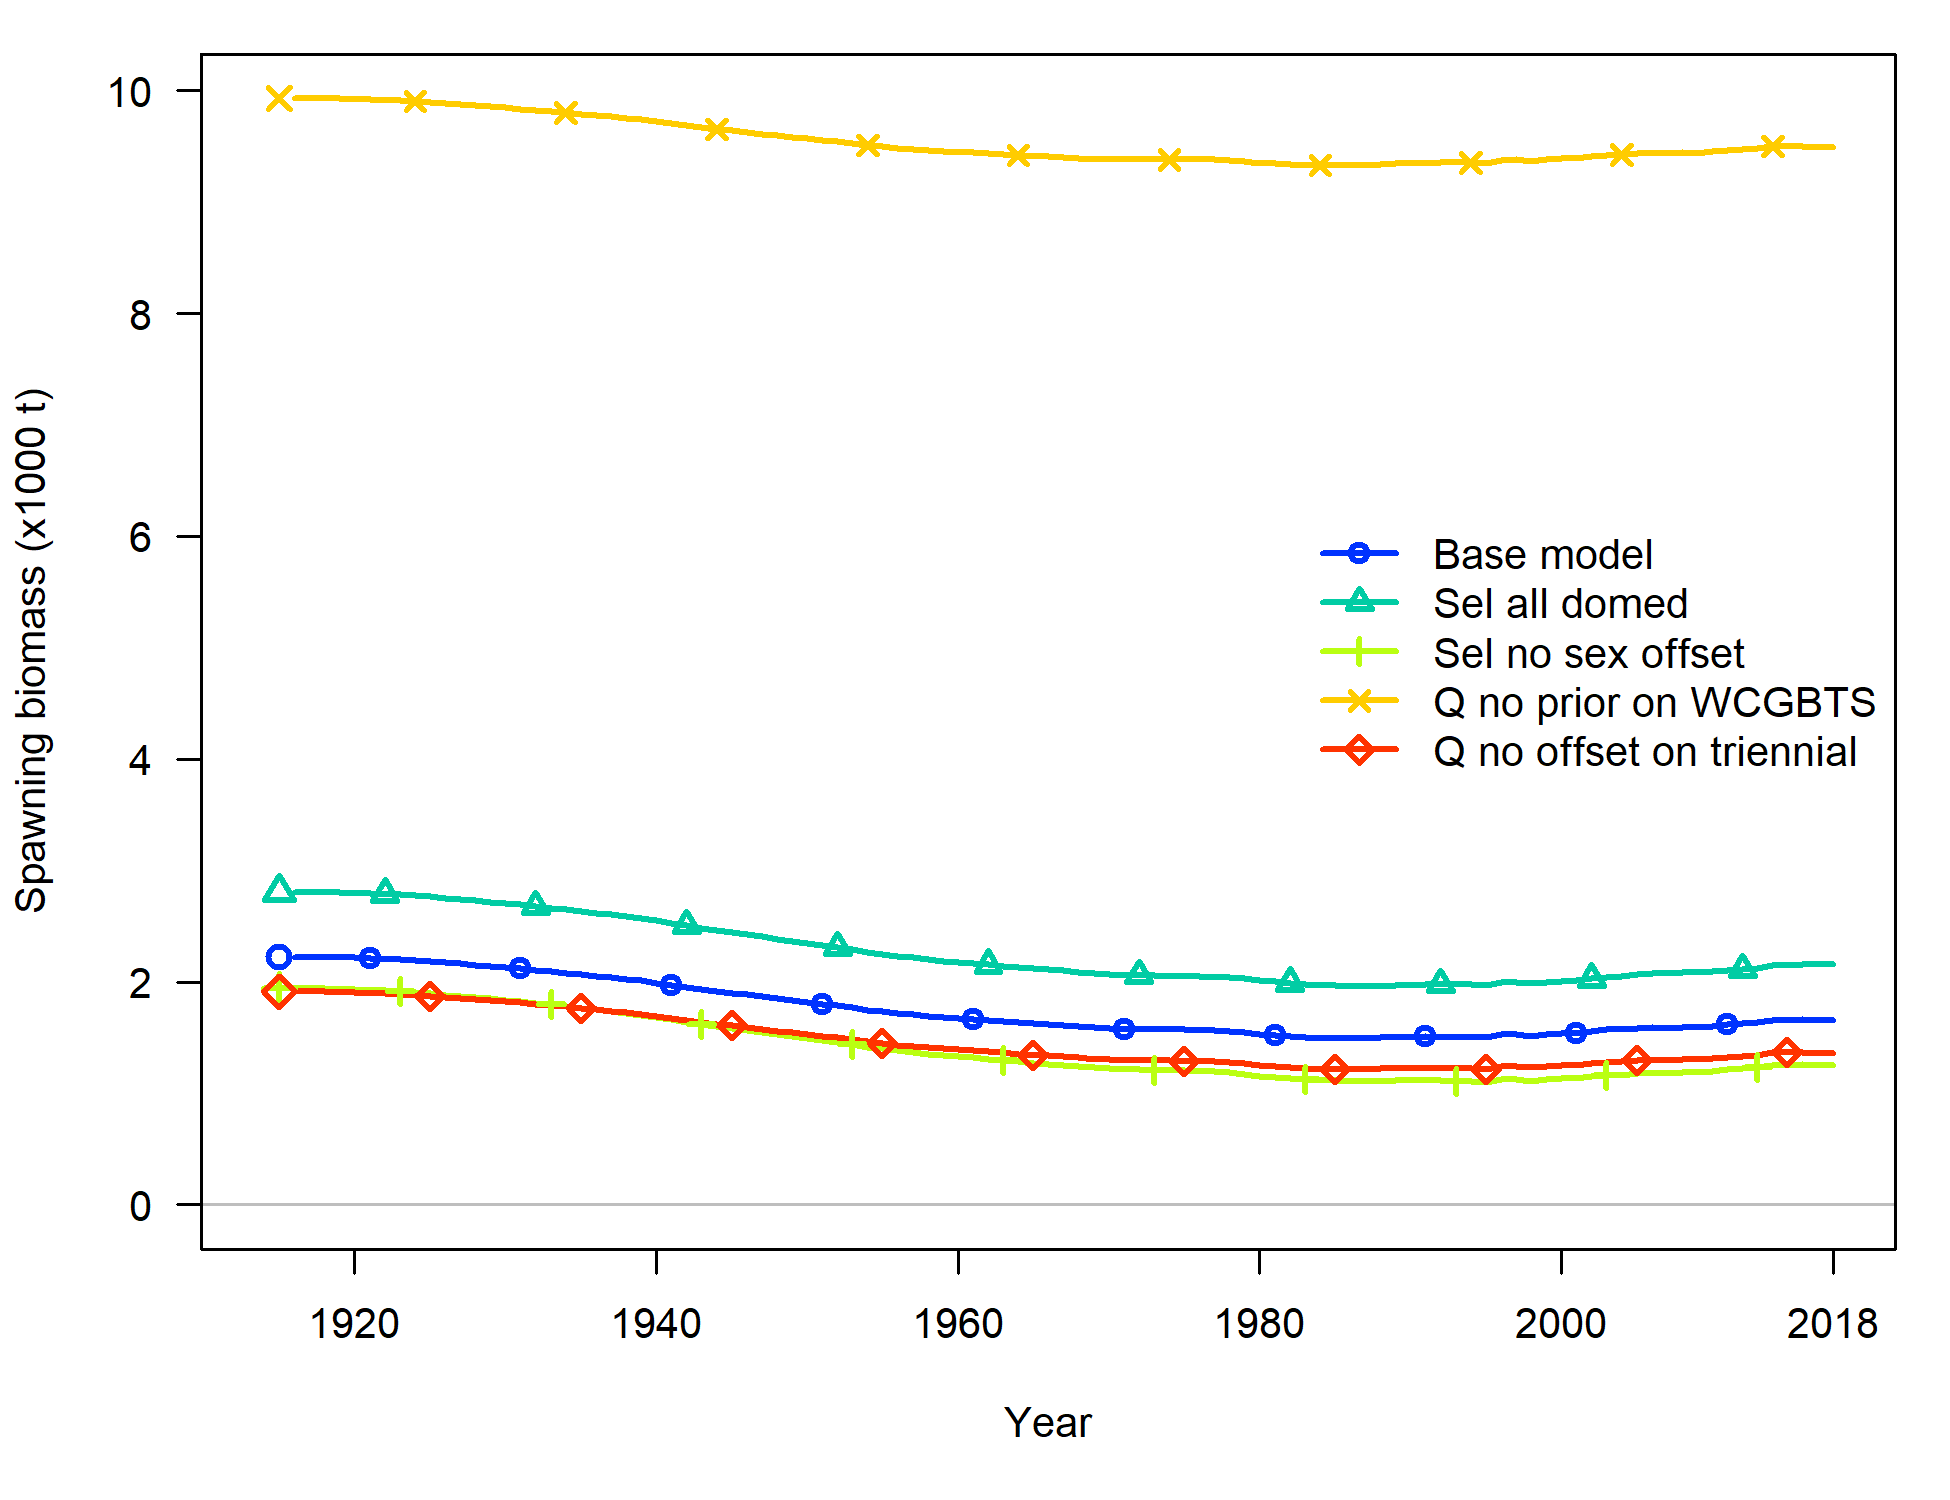
\includegraphics{Figures/sens.sel_and_Q_compare1_spawnbio.png}
\caption{Time series of spawning biomass (mt) estimated in sensitivity analyses related to selectivity and catchability.}\label{fig:Sensitivity_sel_and_Q}
\end{centering}
\end{figure}

\newpage

\begin{figure}
\centering
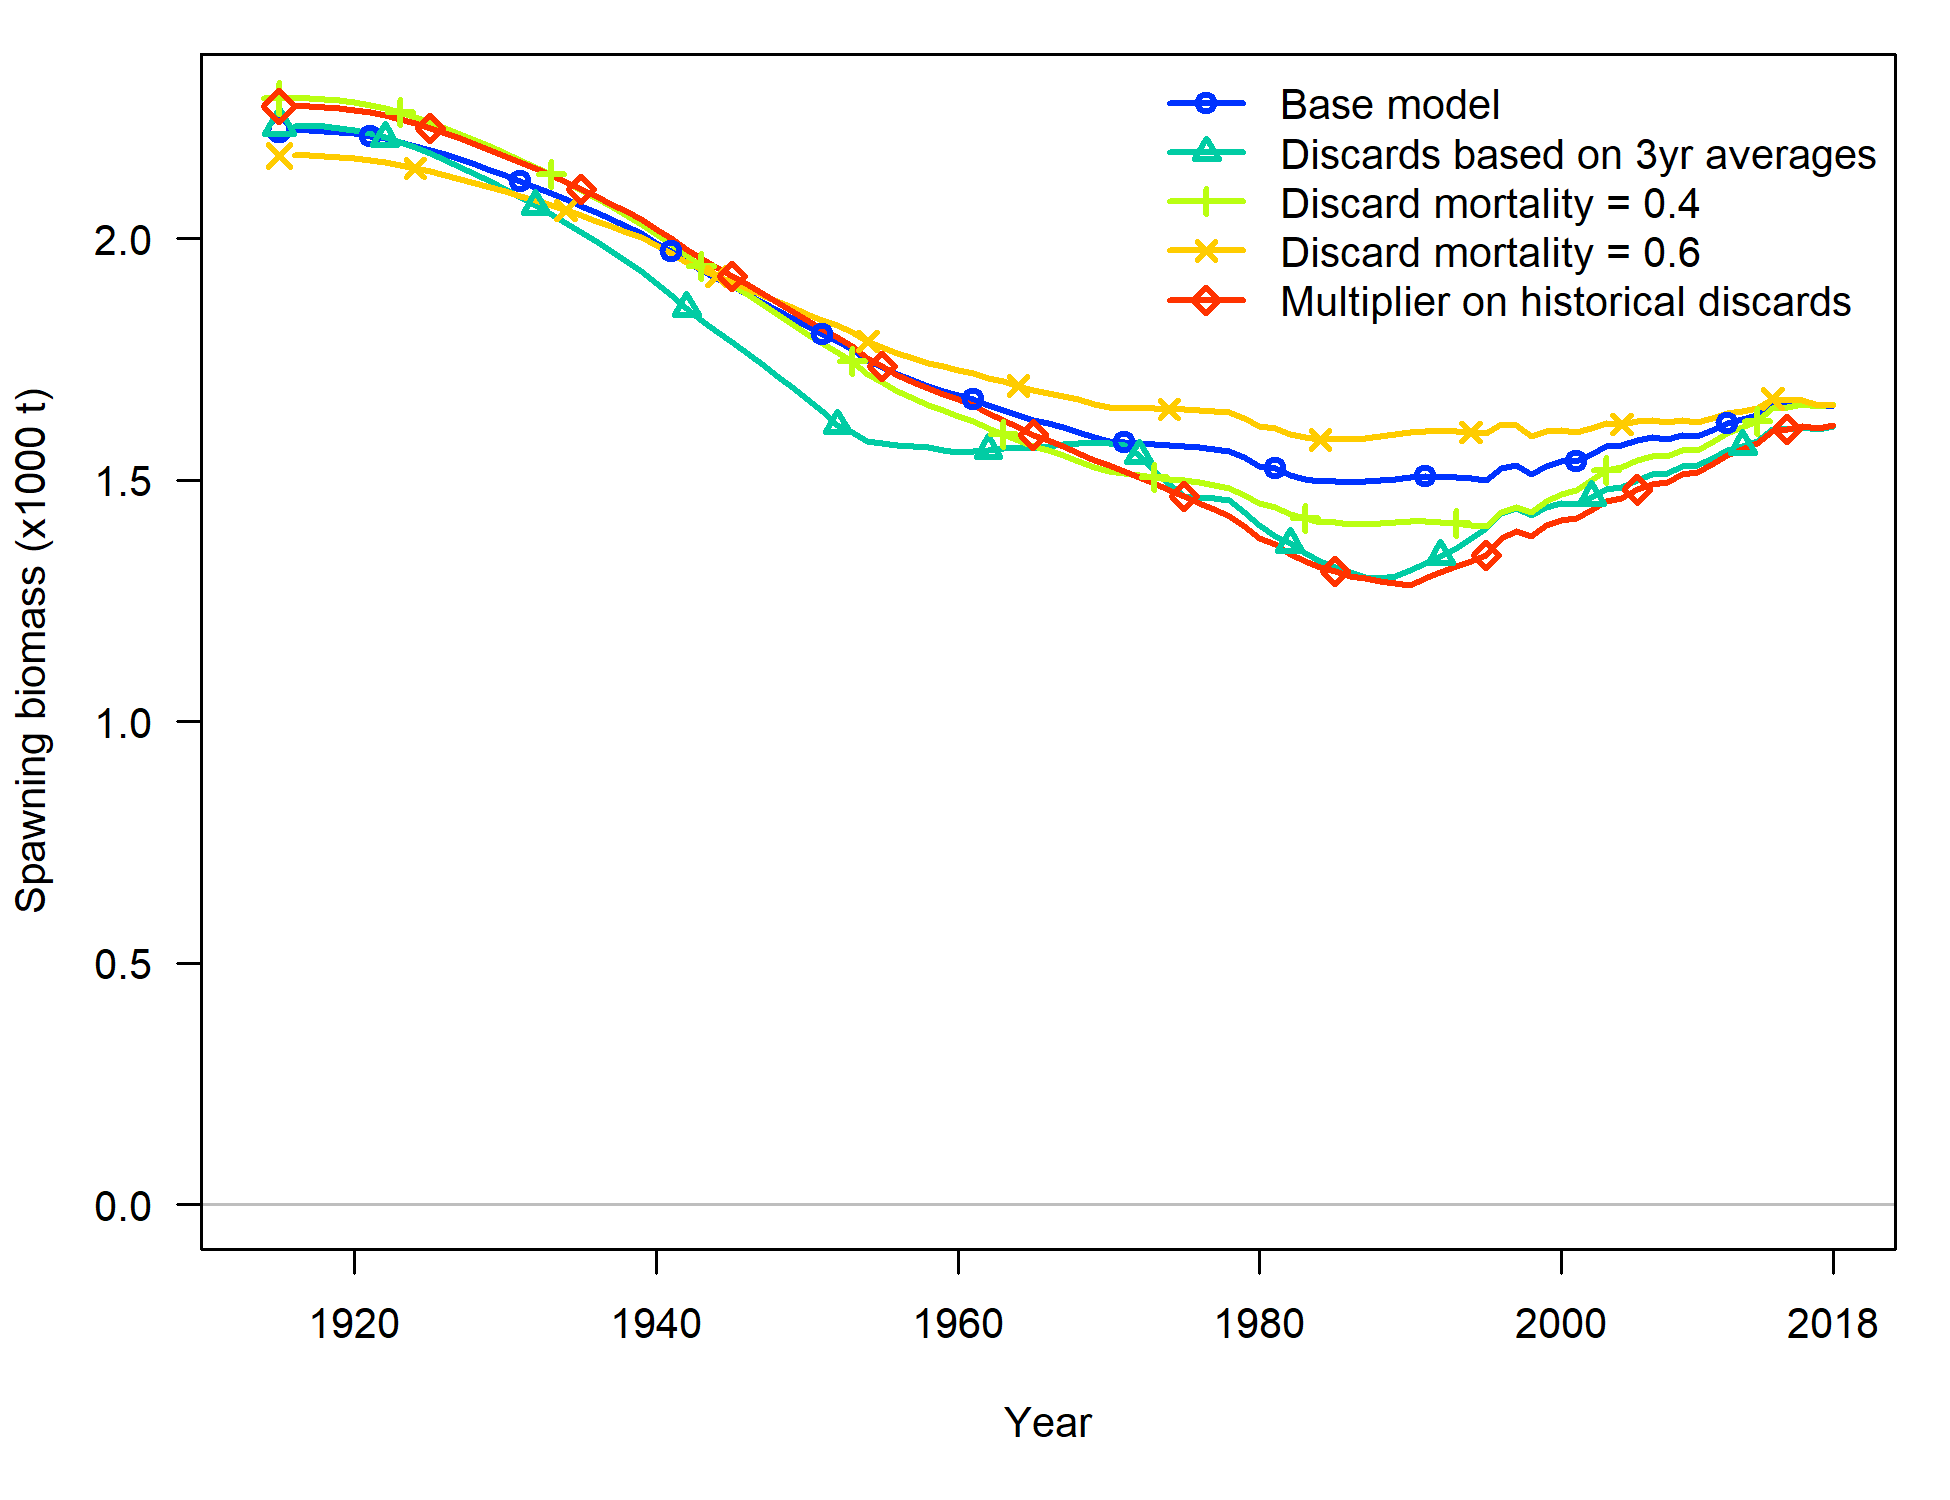
\includegraphics{Figures/sens.catch_compare1_spawnbio.png}
\caption{Time series of spawning biomass (mt) estimated in sensitivity
analyses related to historic catch and discards.
\label{fig:Sensitivity_catch}}
\end{figure}

\begin{figure}
\centering
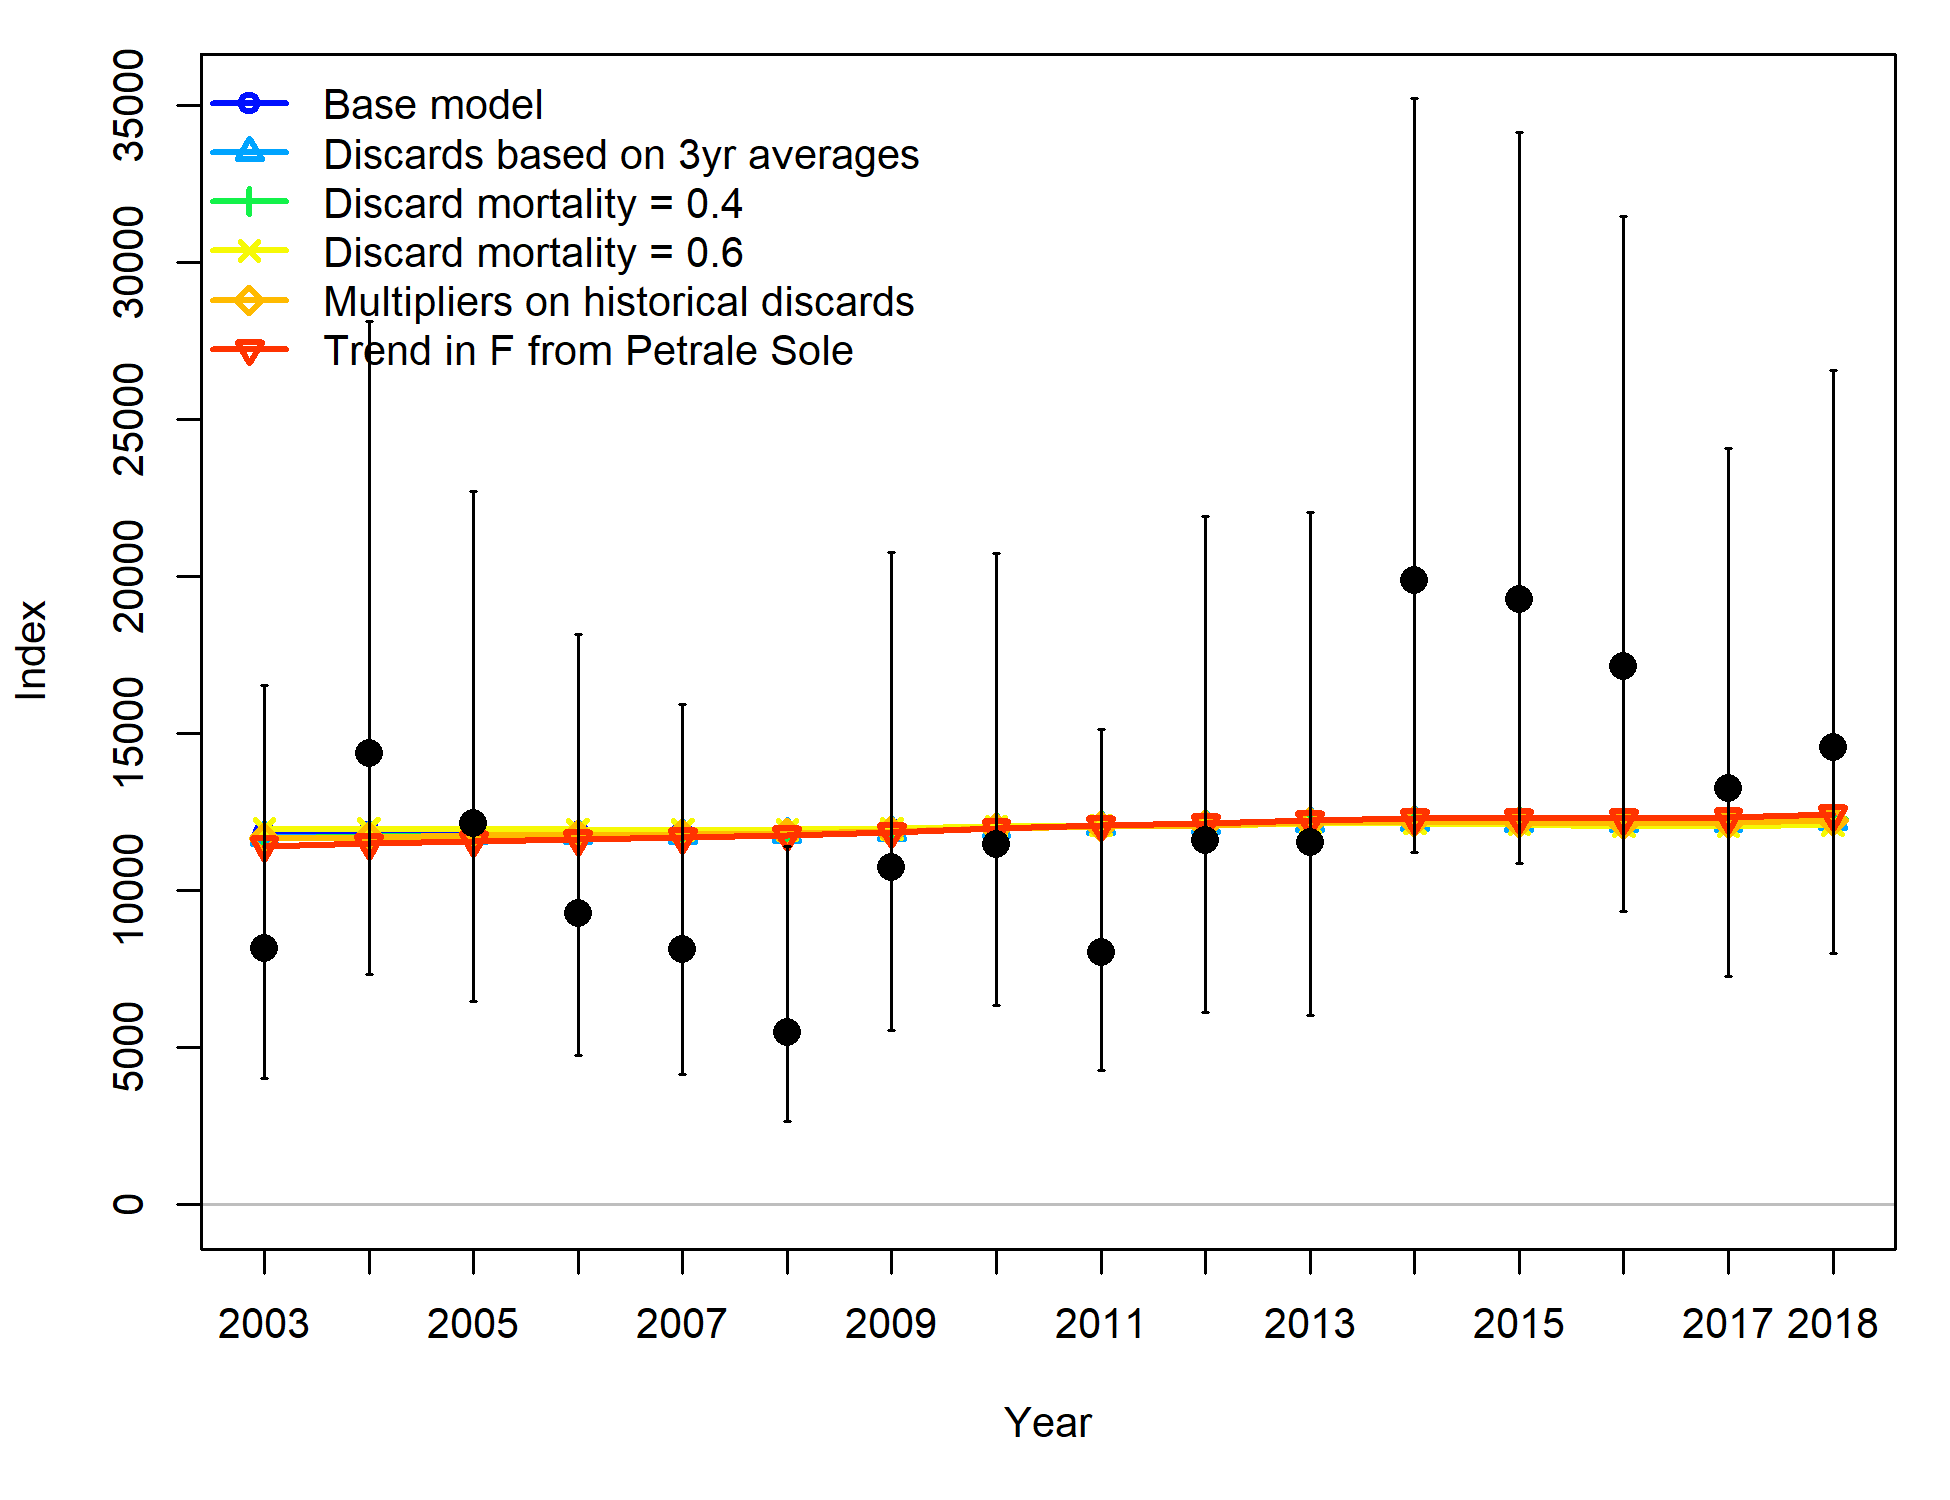
\includegraphics{Figures/sens.catch_compare11_indices_flt5.png}
\caption{Fit to the WCGBT Survey estimated in the sensitivity analyses
related to historic catch and discards. \label{fig:Sensitivity_catch2}}
\end{figure}

\begin{figure}
\centering
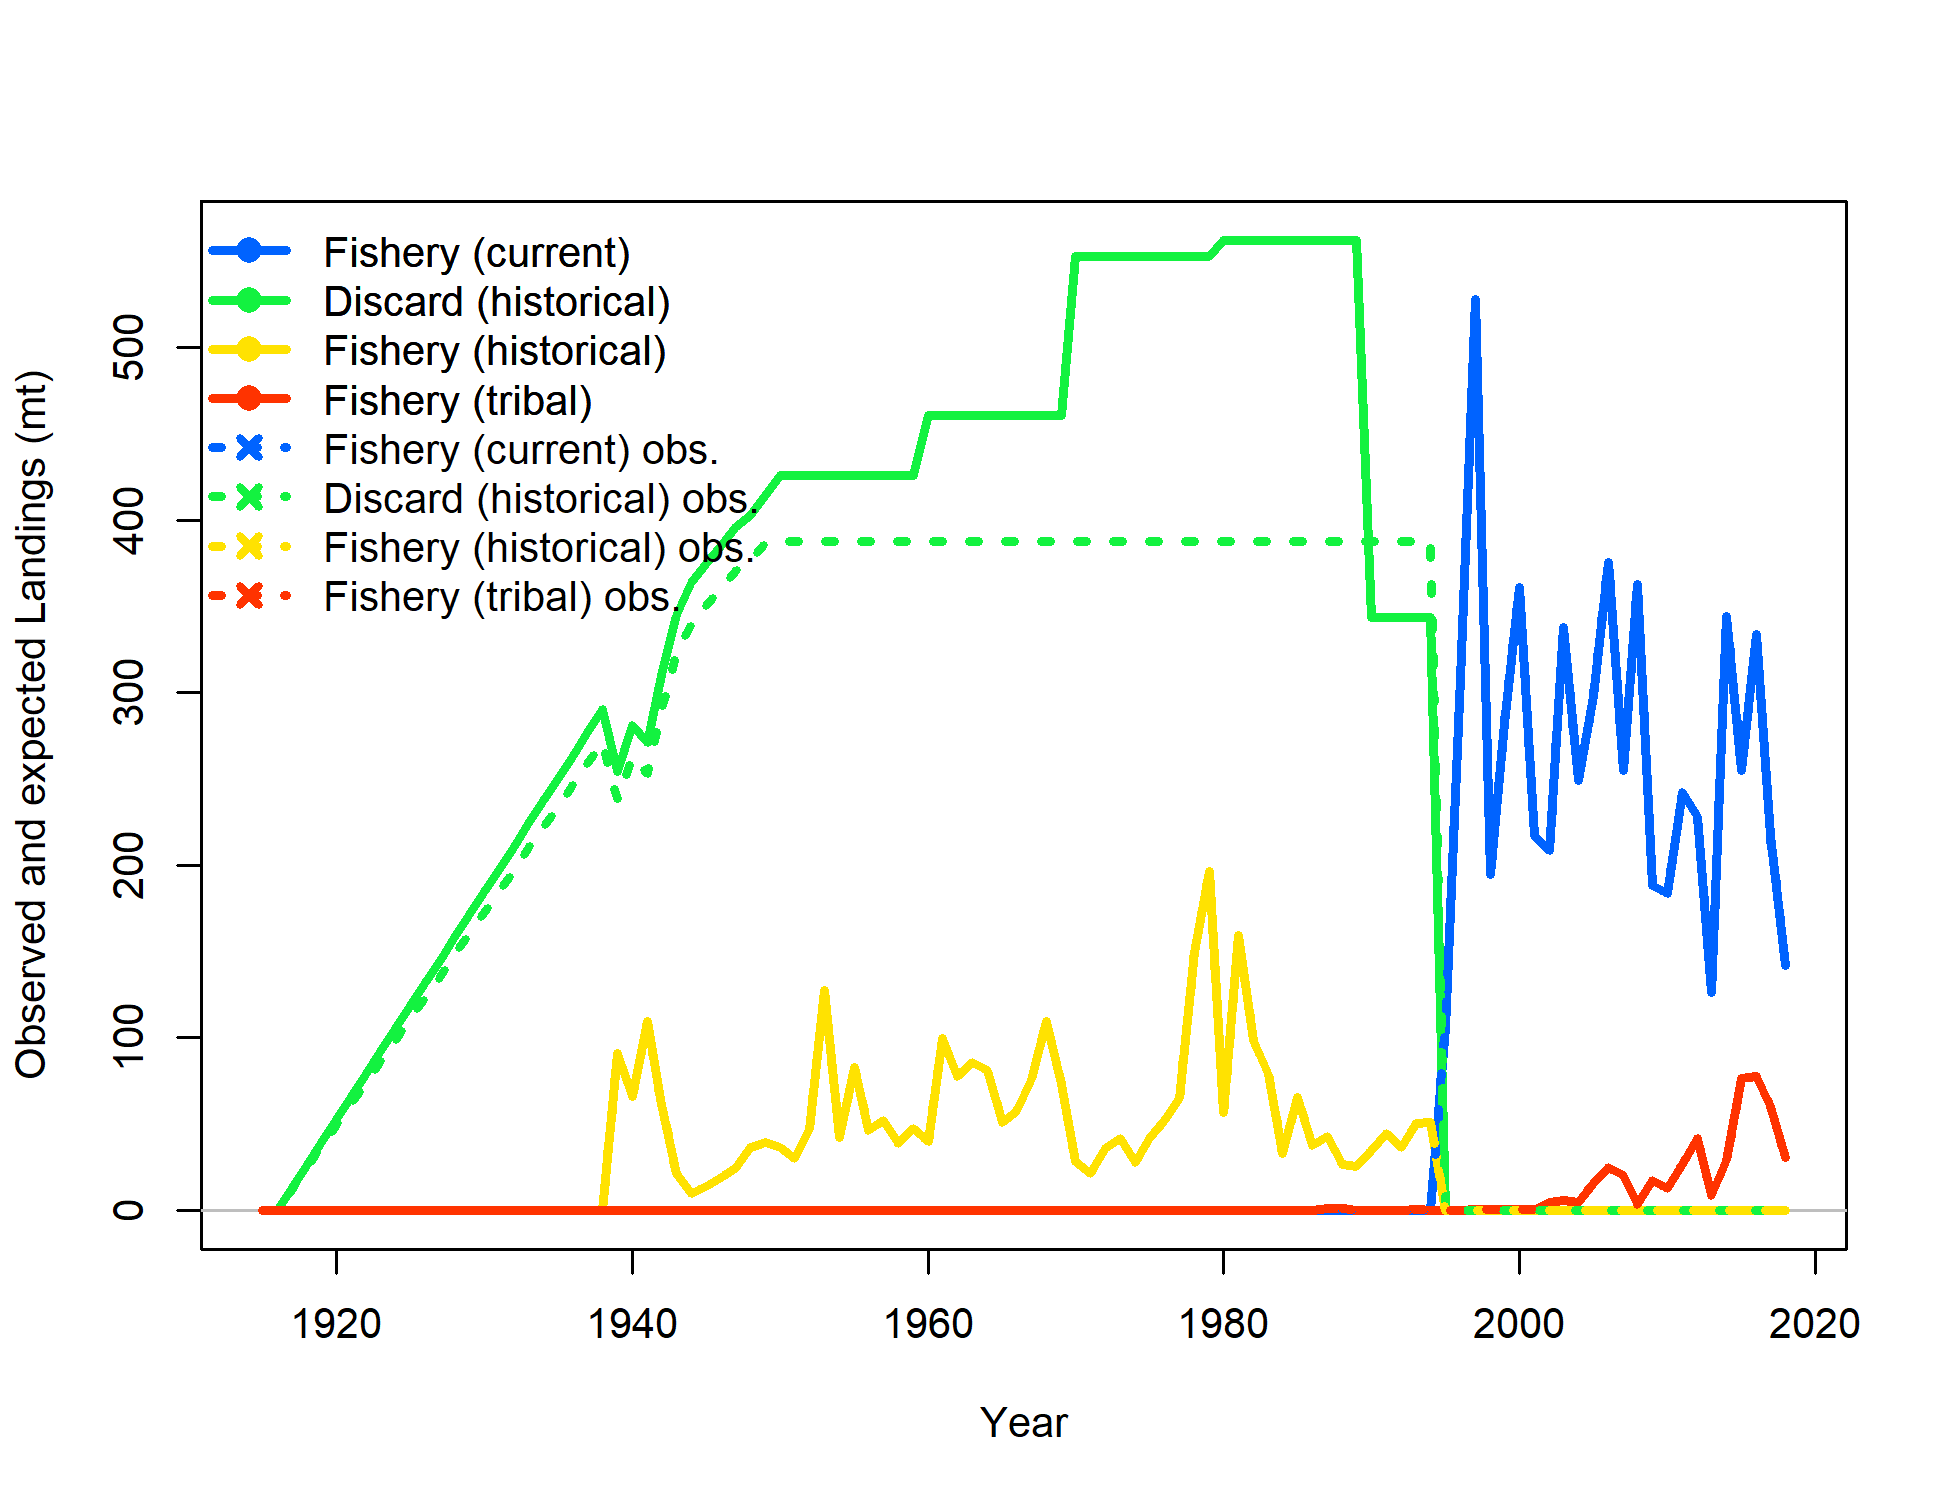
\includegraphics{Figures/catch_multiplier_catch_comparison.png}
\caption{Catch by category for the sensitivity analysis where
multipliers on historical discards were estimated. The estimated time
series including the multipliers is shown in the solid green line and
the input values in the base model are shown in the dashed green line.
\label{fig:catch_multiplier_catch_comparison}}
\end{figure}

\begin{figure}
\centering
\includegraphics{Figures/catch_multiplier_total_catch.png}
\caption{Estimated total catch for the sensitivity analysis where
multipliers on historical discards were estimated. The historical
discards shown in green have been scaled to account for an assumed 50\%
discard mortality but the discards in the recent period show both live
and dead discards. \label{fig:catch_multiplier_total_catch}}
\end{figure}

\begin{figure}
\centering
\includegraphics{Figures/sens.bio_and_misc_compare1_spawnbio.png}
\caption{Time series of spawning biomass (mt) estimated in sensitivity
analyses related to biology and other assumptions.
\label{fig:Sensitivity_bio_and_misc}}
\end{figure}

\begin{figure}
\centering
\includegraphics{Figures/growth_curve_comparison.png}
\caption{Comparison of the estimated growth curves from the
sensitivities analyses. The increase at age 20 in the von Bertalanffy
and Richards growth models is an adjustment to account for average size
in the plus group based on an assumed exponential decay of the numbers
at age beyond age 20.\label{fig:growth_curve_comparison}}
\end{figure}

\FloatBarrier

\begin{figure}
\centering
\includegraphics{Figures/retro_compare2_spawnbio_uncertainty.png}
\caption{Time series of spawning biomass (mt) with approximate 95\%
asymptotic intervals estimated in retrospective analyses in which the
final 5 years of data are successively removed from the
model.\label{fig:retro}}
\end{figure}

\newpage

\hypertarget{likelihood-profiles-1}{%
\subsubsection{Likelihood Profiles}\label{likelihood-profiles-1}}

\FloatBarrier

\vspace{.5cm}

\begin{figure}[h]
\begin{centering}
\includegraphics{Figures/profile_logR0.png}
\caption{Likelihood profile over the log of equilibrium recruitment ($R_0$).}\label{fig:profile_logR0}
\end{centering}
\end{figure}

\newpage

\begin{figure}
\centering
\includegraphics{Figures/profile_logR0.png}
\caption{Likelihood profile over the log of equilibrium recruitment
(\(R_0\)).\label{fig:profile_logR0}}
\end{figure}

\begin{figure}
\centering
\includegraphics{Figures/profile_R0_compare1_spawnbio.png}
\caption{Time series of spawning biomass (mt) estimated for the models
included in the profile over the log of equilibrium recruitment
(\(R_0\)).\label{fig:profile_R0_compare1_spawnbio}}
\end{figure}

\FloatBarrier

\begin{figure}
\centering
\includegraphics{Figures/profile_h.png}
\caption{Likelihood profile over stock-recruit steepness (\(h\)).
\label{fig:profile_h}}
\end{figure}

\begin{figure}
\centering
\includegraphics{Figures/profile_h_compare1_spawnbio.png}
\caption{Time series of spawning biomass (mt) estimated for the models
included in the profile over stock-recruit steepness (\(h\)).
\label{fig:profile_h_compare1_spawnbio}}
\end{figure}

\FloatBarrier

\begin{figure}
\centering
\includegraphics{Figures/profile_M.png}
\caption{Likelihood profile over natural mortality (\(M\)).
\label{fig:profile_M}}
\end{figure}

\begin{figure}
\centering
\includegraphics{Figures/profile_M_compare1_spawnbio.png}
\caption{Time series of spawning biomass (mt) estimated for the models
included in the profile over natural mortality (\(M\)).
\label{fig:profile_M_compare1_spawnbio}}
\end{figure}

\FloatBarrier

\hypertarget{reference-points-and-forecasts}{%
\subsubsection{Reference Points and
Forecasts}\label{reference-points-and-forecasts}}

\FloatBarrier

\vspace{.5cm}

\begin{figure}[h]
\begin{centering}
\includegraphics{r4ss/plots_mod1/yield1_yield_curve.png}
\caption{Equilibrium yield curve for the base case model. Values are based on the fishery selectivity and with steepness fixed at 0.4.}\label{fig:yield1_yield_curve}
\end{centering}
\end{figure}

\newpage

\FloatBarrier

\newpage

\FloatBarrier
\newpage

\hypertarget{appendix-a.-detailed-fits-to-length-composition-data}{%
\section*{Appendix A. Detailed fits to length composition
data}\label{appendix-a.-detailed-fits-to-length-composition-data}}
\addcontentsline{toc}{section}{Appendix A. Detailed fits to length
composition data}

\renewcommand{\thepage}{A-\arabic{page}}
\renewcommand{\thefigure}{A\arabic{figure}}
\setcounter{page}{1}

\begin{figure}
\centering
\includegraphics{./r4ss/plots_mod1/comp_lenfit_flt1mkt2.png}
\caption{Length comps, retained, Fishery. `N adj.' is the input sample
size after data\_weighting adjustment. N eff. is the calculated
effective sample size used in the McAllister\_Iannelli tuning method.
\label{fig:mod1_1_comp_lenfit_flt1mkt2}}
\end{figure}

\begin{figure}
\centering
\includegraphics{./r4ss/plots_mod1/comp_lenfit_flt1mkt1.png}
\caption{Length comps, discard, Fishery. `N adj.' is the input sample
size after data\_weighting adjustment. N eff. is the calculated
effective sample size used in the McAllister\_Iannelli tuning method.
\label{fig:mod1_2_comp_lenfit_flt1mkt1}}
\end{figure}

\begin{figure}
\centering
\includegraphics{./r4ss/plots_mod1/comp_lenfit_flt5mkt0.png}
\caption{Length comps, whole catch, WCGBT Survey. `N adj.' is the input
sample size after data\_weighting adjustment. N eff. is the calculated
effective sample size used in the McAllister\_Iannelli tuning method.
\label{fig:mod1_3_comp_lenfit_flt5mkt0}}
\end{figure}

\begin{figure}
\centering
\includegraphics{./r4ss/plots_mod1/comp_lenfit_flt6mkt0.png}
\caption{Length comps, whole catch, Triennial Survey. `N adj.' is the
input sample size after data\_weighting adjustment. N eff. is the
calculated effective sample size used in the McAllister\_Iannelli tuning
method. \label{fig:mod1_4_comp_lenfit_flt6mkt0}}
\end{figure}

\newpage

\color{black}

\hypertarget{references}{%
\section*{References}\label{references}}
\addcontentsline{toc}{section}{References}

\renewcommand{\thepage}{}

\hypertarget{refs}{}
\leavevmode\hypertarget{ref-AFSC2018}{}%
Alaska Fisheries Science Center. 2018. Assessment of the skate stock
complex in the Gulf of Alaska. Available from
\href{\%7Bhttps://www.afsc.noaa.gov/REFM/Docs/2018/GOA/GOAskate.pdf\%7D}{\{https://www.afsc.noaa.gov/REFM/Docs/2018/GOA/GOAskate.pdf\}}.

\leavevmode\hypertarget{ref-Batdorf1990}{}%
Batdorf, C. 1990. Northwest Native Harvest. Hancock House Publishers
Ltd.; Surrey, B.C., Canada.

\leavevmode\hypertarget{ref-Bizzarro2015}{}%
Bizzarro, J. 2015. Comparative resource utilization of eastern north
pacific skates (rajiformes: Rajidae) with applications for
ecosystem-based fisheries management. WA: University of Washington.

\leavevmode\hypertarget{ref-Bizzarro2019}{}%
Bizzarro, J. 2019. Manuscript in preparation.

\leavevmode\hypertarget{ref-Bizzarro2014}{}%
Bizzarro, JJ and Broms, KM and Logsdon, MG and Ebert, DA and Yoklavich,
MM and Kuhnz, LA and Summers, AP. 2014. Spatial segregation in eastern
north Pacific skate assemblages. PloS one \textbf{9}(10).

\leavevmode\hypertarget{ref-Bizzarro2007}{}%
Bizzarro, J., Robinson, H., Rinewalt, C., and Ebert, D. 2007.
Comparative feeding ecology of four sympatric skate species off central
California, USA. \emph{In} Biology of skates. Springer. pp. 91--114.

\leavevmode\hypertarget{ref-Bowers1909}{}%
Bowers, G. M. 1909. Report of The Commissioner For the Year Ending June
30, 1909. Part XXVIII. Washington Printing Office.

\leavevmode\hypertarget{ref-Bradburn2011}{}%
Bradburn, M.J. and Keller, A.A and Horness, B.H. 2011. The 2003 to 2008
US West Coast bottom trawl surveys of groundfish resources off
Washington, Oregon, and California: estimates of distribution,
abundance, length, and age composition. NOAA Technical Memorandum NMFS
NOAA-TM-NMFS-NWFSC-114: 323 pp.

\leavevmode\hypertarget{ref-brown2001interval}{}%
Brown, L.D., Cai, T.T., and DasGupta, A. 2001. Interval estimation for a
binomial proportion. Statistical science: 101--117. JSTOR.

\leavevmode\hypertarget{ref-TedCalavan}{}%
Calavan, T. 2019. Oregon Department of Fisheries; Wildlife; Personal
Communication, Newport, OR, USA.

\leavevmode\hypertarget{ref-Castro1996}{}%
Castro-Aguirre, J.L., and Pérez, H.E. 1996. Catálogo sistemático de las
rayas y especies afines de méxico: Chondrichthyes: Elasmobranchii:
Rajiformes: Batoideiomorpha. Unam.

\leavevmode\hypertarget{ref-Castro1993}{}%
Castro-Aguirre, J., Schmitter, J., Balart, E., and Torres-Orozco, R.
1993. Sobre la distribución geográfica de algunos peces bentónicos de la
costa oeste de baja california sur, méxico, con consideraciones
ecológicas y evolutivas. \emph{In} Anales de la escuela nacional de
ciencias biológicas, méxico. pp. 75--102.

\leavevmode\hypertarget{ref-Chapman1944}{}%
Chapman, W.M. 1944. The Latent Fisheries of Washington and Alaska.
Washington State Department of Fisheries.

\leavevmode\hypertarget{ref-Chiquillo2014}{}%
Chiquillo, Kelcie L and Ebert, David A and Slager, Christina J and Crow,
Karen D. 2014. The secret of the mermaid's purse: Phylogenetic
affinities within the Rajidae and the evolution of a novel reproductive
strategy in skates. Molecular Phylogenetics and Evolution \textbf{75}:
245--251. Elsevier.

\leavevmode\hypertarget{ref-DeLacy1935}{}%
DeLacy, A.C., and Chapman, W.M. 1935. Notes on some elasmobranchs of
puget sound, with descriptions of their egg cases. Copeia
\textbf{1935}(2): 63--67. JSTOR.

\leavevmode\hypertarget{ref-Dorn2007}{}%
Dorn, M and Cordue, P and Haist, V. 2007. Pacific Fishery Management
Council, Portland, OR. Available from
\href{\%7B\%7Bhttps://www.pcouncil.org/wp-content/uploads/STARreport_Skate.pdf\%7D\%7D}{\{\{https://www.pcouncil.org/wp-content/uploads/STARreport\_Skate.pdf\}\}}.

\leavevmode\hypertarget{ref-Downs2013}{}%
Downs, D.E., and Cheng, Y.W. 2013. Length--length and width--length
conversion of longnose skate and big skate off the pacific coast:
Implications for the choice of alternative measurement units in
fisheries stock assessment. North American journal of fisheries
management \textbf{33}(5): 887--893. Taylor \& Francis.

\leavevmode\hypertarget{ref-Ebert2003}{}%
Ebert, D. 2003. Sharks, rays, and chimaeras of california. Univ of
California Press.

\leavevmode\hypertarget{ref-Ebert2007}{}%
Ebert, D.A., and Compagno, L.J. 2007. Biodiversity and systematics of
skates (chondrichthyes: Rajiformes: Rajoidei). \emph{In} Biology of
skates. Springer. pp. 5--18.

\leavevmode\hypertarget{ref-Ebert2008}{}%
Ebert, D.A., Smith, W.D., and Cailliet, G.M. 2008. Reproductive biology
of two commercially exploited skates, raja binoculata and r. Rhina, in
the western gulf of alaska. Fisheries Research \textbf{94}(1): 48--57.
Elsevier.

\leavevmode\hypertarget{ref-Eschmeyer1983}{}%
Eschmeyer, W.N., and Herald, E.S. 1983. A field guide to pacific coast
fishes: North america. Houghton Mifflin Harcourt.

\leavevmode\hypertarget{ref-Farrugia2016}{}%
Farrugia, T.J., Goldman, K.J., Tribuzio, C., and Seitz, A.C. 2016. First
use of satellite tags to examine movement and habitat use of big skates
beringraja binoculata in the gulf of alaska. Marine Ecology Progress
Series \textbf{556}: 209--221.

\leavevmode\hypertarget{ref-Ford1971}{}%
Ford, P. 1971. Differential growth rate in the tail of the pacific big
skate, (\emph{Raja binoculata}). Journal of the Fisheries Board of
Canada \textbf{28}(1): 95--98. NRC Research Press.

\leavevmode\hypertarget{ref-Francis2011}{}%
Francis, R.I.C.C. 2011. Data weighting in statistical fisheries stock
assessment models. Canadian Journal of Fisheries and Aquatic Sciencies
\textbf{68}: 1124--1138.

\leavevmode\hypertarget{ref-Gburski2007}{}%
Gburski, C.M. and Gaichas, S.K. and Kimura, D.K. 2007. Age and growth of
big skate (\emph{Raja binoculata}) and longnose skate (\emph{Raja
rhina}) in the Gulf of Alaska. \emph{In} Biology of Skates. Springer,
Dordrecht.

\leavevmode\hypertarget{ref-Gertseva2019}{}%
Gertseva, V. 2019. Manuscript in preparation.

\leavevmode\hypertarget{ref-Gertseva2007}{}%
Gertseva, V and Schrippa, MJ. 2007. Status of the Longnose Skate
(\emph{Raja rhina}) off the continental US Pacific Coast in 2007.
Pacific Fishery Management Council, Portland, OR. Available from
\href{\%7Bhttp://www.pcouncil.org/groundfish/stock-assessments/\%7D}{\{http://www.pcouncil.org/groundfish/stock-assessments/\}}.

\leavevmode\hypertarget{ref-Gertseva2011}{}%
Gertseva, V., and Taylor, I. 2011. Status of spiny dogfish shark
resource off the continental us pacific coast in 2011. PFMC. 2011.
Pacific Fishery Management Council, Portland, OR. Available from
\href{\%7Bhttp://www.pcouncil.org/groundfish/stock-assessments/\%7D}{\{http://www.pcouncil.org/groundfish/stock-assessments/\}}.

\leavevmode\hypertarget{ref-Gunderson1980}{}%
Gunderson, Donald Raymond and Sample, Terrance M. 1980. Distribution and
abundance of rockfish off Washington, Oregon and California during 1977.
Northwest and Alaska Fisheries Center, National Marine Fisheries
Service. Available from
\href{\%7Bhttp://spo.nmfs.noaa.gov/mfr423-4/mfr423-42.pdf\%7D}{\{http://spo.nmfs.noaa.gov/mfr423-4/mfr423-42.pdf\}}.

\leavevmode\hypertarget{ref-Hamel2015}{}%
Hamel, Owen S. 2015. A method for calculating a meta-analytical prior
for the natural mortality rate using multiple life history correlates.
ICES Journal of Marine Science: Journal du Conseil \textbf{72}(1):
62--69. doi:
\href{https://doi.org/\%7B10.1093/icesjms/fsu131\%7D}{\{10.1093/icesjms/fsu131\}}.

\leavevmode\hypertarget{ref-Hitz1964}{}%
Hitz, C.R. 1964. Observations on egg cases of the big skate (raja
binoculata girard) found in oregon coastal waters. Journal of the
Fisheries Board of Canada \textbf{21}(4): 851--854. NRC Research Press.

\leavevmode\hypertarget{ref-Hoff2009}{}%
Hoff, GR. 2009. Skate Bathyraja spp. egg predation in the eastern Bering
Sea. J. Fish. Biol. \textbf{74}: 250--269.

\leavevmode\hypertarget{ref-Ishihara2012}{}%
Ishihara, H., Treloar, M., Bor, P., Senou, H., and Jeong, C. 2012. The
comparative morphology of skate egg capsules (Chondrichthyes:
Elasmobranchii: Rajiformes). Bulletin of the Kanagawa Prefectural Museum
(Natural Science) \textbf{41}: 9--25.

\leavevmode\hypertarget{ref-Keller2017}{}%
Keller, A.A. and Wallace, J.R. and Methot, R.D. 2017. The Northwest
Fisheries Science Center's West Coast Groundfish Bottom Trawl Survey:
History, Design, and Description. NOAA Technical Memorandum NMFS
NOAA-TM-NMFS-NWFSC-136: 38 pp.

\leavevmode\hypertarget{ref-KingandMcF2009}{}%
King, J., and McFarlane, G. 2009. Biological results of the strait of
georgia spiny dogfish (squalus acanthias) longline survey, october
10-22, 2008. Fisheries; Oceans Canada, Science Branch, Pacific Region.

\leavevmode\hypertarget{ref-King2015}{}%
King, J.R., Surry, A.M., Garcia, S., and P.J. Starr. 2015. Big skate
(Raja binoculata) and longnose skate (R. rhina) stock assessments for
British Columbia. Ottawa : Canadian Science Advisory Secretariat.

\leavevmode\hypertarget{ref-KingandMcF2010}{}%
King, JR and McFarlane, GA. 2010. Movement patterns and growth estimates
of big skate (\emph{Raja binoculata}) based on tag-recapture data. Fish.
Res. \textbf{101}: 50--59.

\leavevmode\hypertarget{ref-GregLippert}{}%
Lippert, G. 2019. Washington Department of Fisheries; Wildlife; Personal
Communication, Olympia, Washington, USA.

\leavevmode\hypertarget{ref-Love2011}{}%
Love, Milton S. 2011. Certainly more than you want to know about the
fishes of the Pacific Coast: a postmodern experience. Really Big Press.

\leavevmode\hypertarget{ref-maunder2018growth}{}%
Maunder, M.N., Deriso, R.B., Schaefer, K.M., Fuller, D.W.,
Aires-da-Silva, A.M., Minte-Vera, C.V., and Campana, S.E. 2018. The
growth cessation model: A growth model for species showing a near
cessation in growth with application to bigeye tuna (thunnus obesus).
Marine biology \textbf{165}(4): 76. Springer.

\leavevmode\hypertarget{ref-McEachran1990}{}%
McEachran, J., and Miyake, T. 1990. 1990. Zoogeography and bathymetry of
skates (chondrichthyes, rajidae). Elasmobranchs as living resources.
Advances in biology, Ecology, Systematics and the status of the
fisheries: 305--326.

\leavevmode\hypertarget{ref-McFandKing2006}{}%
McFarlane GA and King JR. 2006. Age and growth of big skate (\emph{Raja
binoculata}) and longnose skate (\emph{Raja rhina}) in British Columbia
waters. Fisheries Research \textbf{May 1 (2-3)}: 169--78.

\leavevmode\hypertarget{ref-Mecklenburg2002}{}%
Mecklenburg, CW and Mecklenburg, TA and Thorsteinson, LK. 2002. Fishes
of Alaska. American Fisheries Society, Bethesda, Maryland.

\leavevmode\hypertarget{ref-Methot2019}{}%
Methot, RD Jr. and Wetzel, CR and Taylor, IG. 2019. Stock Synthesis User
Manual Version 3.30.13. NOAA Fisheries. Seattle, WA. Available from
\href{\%7Bhttps://vlab.ncep.noaa.gov/web/stock-synthesis\%7D}{\{https://vlab.ncep.noaa.gov/web/stock-synthesis\}}.

\leavevmode\hypertarget{ref-Methot2013}{}%
Methot, Richard D. and Wetzel, Chantell R. 2013. Stock synthesis: A
biological and statistical framework for fish stock assessment and
fishery management. Fisheries Research \textbf{142}: 86--99.

\leavevmode\hypertarget{ref-Miller1980}{}%
Miller, B.S., Cross, J.N., Steinfort, S.N., Fresh, K.L., and Simenstad,
C.A. 1980. Nearshore fish and macroinvertebrate assemblages along the
strait of juan de fuca including food habits of the common nearshore
fish.

\leavevmode\hypertarget{ref-PFMC2018}{}%
Pacific Fishery Management Council. 2018. Status of the Pacific Coast
Groundfish Fishery. Available from
\href{\%7Bhttp://www.pcouncil.org/wp-content/uploads/2017/02/SAFE_Dec2016_02_2\%7D}{\{http://www.pcouncil.org/wp-content/uploads/2017/02/SAFE\_Dec2016\_02\_2\}}.

\leavevmode\hypertarget{ref-Punt2008}{}%
Punt AE and Smith DC and KrusicGolub K and Robertson S. 2008.
Quantifying age-reading error for use in fisheries stock assessments,
with application to species in Australia's southern and eastern
scalefish and shark fishery. Canadian Journal of Fisheries and Aquatic
Sciences.

\leavevmode\hypertarget{ref-richards1959flexible}{}%
Richards, F. 1959. A flexible growth function for empirical use. Journal
of experimental Botany \textbf{10}(2): 290--301. Oxford University
Press.

\leavevmode\hypertarget{ref-Stevenson2008}{}%
Stevenson, DE and Orr, JW and Hoff, GR and McEachran, JD. 2008. Emerging
patterns of species richness, diversity, population density, and
distribution in the skates (Rajidae) of Alaska. Fish Bull \textbf{106}:
24--39.

\leavevmode\hypertarget{ref-Stewart2009}{}%
Stewart, I.J., Wallace, J.R., and McGilliard, C. 2009. Status of the us
yelloweye rockfish resource in 2009. \emph{In} Pacific Fishery
Management Council, Portland, OR. Available from
\href{\%7Bhttp://www.pcouncil.org/groundfish/stock-assessments/\%7D}{\{http://www.pcouncil.org/groundfish/stock-assessments/\}}.

\leavevmode\hypertarget{ref-Taylor2019}{}%
Taylor, I.G., Stewart, I.J., Hicks, A.C., Garrison, T.M., Punt, A.E.,
Wallace, J.R., Wetzel, C.R., Thorson, J.T., Takeuchi, Y., Ono, K.,
Monnahan, C.C., Stawitz, C.C., A'mar, Z.T., Whitten, A.R., Johnson,
K.F., Emmet, R.L., Anderson, S.C., Lambert, G.I., Stachura, M.M.,
Cooper, A.B., Stephens, A., Klaer, N.L., McGilliard, C.R., Iwasaki,
W.M., Doering, K., and Havron, A.M. 2019. R4ss: R code for stock
synthesis. Available from \url{https://github.com/r4ss}.

\leavevmode\hypertarget{ref-Taylor2013}{}%
Taylor IG and Cope, J and Hamel O and Thorson, J. 2013. Deriving
estimates of OFL for species in the ``Other Fish'' complex or potential
alternative complexes. Pacific Fishery Management Council, Portland, OR.
Available from
\href{\%7Bhttp://www.pcouncil.org/groundfish/stock-assessments/\%7D}{\{http://www.pcouncil.org/groundfish/stock-assessments/\}}.

\leavevmode\hypertarget{ref-Thorson2017a}{}%
Thorson, James T. and Barnett, Lewis A. K. 2017. Comparing estimates of
abundance trends and distribution shifts using single- and multispecies
models of fishes and biogenic habitat. ICES Journal of Marine Science:
Journal du Conseil: fsw193. doi:
\href{https://doi.org/\%7B10.1093/icesjms/fsw193\%7D}{\{10.1093/icesjms/fsw193\}}.

\leavevmode\hypertarget{ref-Thorson2015}{}%
Thorson, J. T. and Shelton, A. O. and Ward, E. J. and Skaug, H. J. 2015.
Geostatistical delta-generalized linear mixed models improve precision
for estimated abundance indices for West Coast groundfishes. ICES
Journal of Marine Science \textbf{72}(5): 1297--1310. doi:
\href{https://doi.org/\%7B10.1093/icesjms/fsu243\%7D}{\{10.1093/icesjms/fsu243\}}.

\leavevmode\hypertarget{ref-VonB}{}%
von Bertalanffy, L. 1938. A quantitative theory of organic growth. Human
Biology \textbf{10}: 181--213.

\leavevmode\hypertarget{ref-ZeinerWolf1993}{}%
Zeiner, S.J. and P. Wolf. 1993. Growth characteristics and estimates of
age at maturity of two species of skates (\emph{Raja binoculata}) and
(\emph{Raja rhina}) from Monterey Bay, California.

\end{document}
